% Options for packages loaded elsewhere
\PassOptionsToPackage{unicode}{hyperref}
\PassOptionsToPackage{hyphens}{url}
%
\documentclass[
]{book}
\usepackage{amsmath,amssymb}
\usepackage{lmodern}
\usepackage{iftex}
\ifPDFTeX
  \usepackage[T1]{fontenc}
  \usepackage[utf8]{inputenc}
  \usepackage{textcomp} % provide euro and other symbols
\else % if luatex or xetex
  \usepackage{unicode-math}
  \defaultfontfeatures{Scale=MatchLowercase}
  \defaultfontfeatures[\rmfamily]{Ligatures=TeX,Scale=1}
\fi
% Use upquote if available, for straight quotes in verbatim environments
\IfFileExists{upquote.sty}{\usepackage{upquote}}{}
\IfFileExists{microtype.sty}{% use microtype if available
  \usepackage[]{microtype}
  \UseMicrotypeSet[protrusion]{basicmath} % disable protrusion for tt fonts
}{}
\makeatletter
\@ifundefined{KOMAClassName}{% if non-KOMA class
  \IfFileExists{parskip.sty}{%
    \usepackage{parskip}
  }{% else
    \setlength{\parindent}{0pt}
    \setlength{\parskip}{6pt plus 2pt minus 1pt}}
}{% if KOMA class
  \KOMAoptions{parskip=half}}
\makeatother
\usepackage{xcolor}
\usepackage{color}
\usepackage{fancyvrb}
\newcommand{\VerbBar}{|}
\newcommand{\VERB}{\Verb[commandchars=\\\{\}]}
\DefineVerbatimEnvironment{Highlighting}{Verbatim}{commandchars=\\\{\}}
% Add ',fontsize=\small' for more characters per line
\usepackage{framed}
\definecolor{shadecolor}{RGB}{248,248,248}
\newenvironment{Shaded}{\begin{snugshade}}{\end{snugshade}}
\newcommand{\AlertTok}[1]{\textcolor[rgb]{0.94,0.16,0.16}{#1}}
\newcommand{\AnnotationTok}[1]{\textcolor[rgb]{0.56,0.35,0.01}{\textbf{\textit{#1}}}}
\newcommand{\AttributeTok}[1]{\textcolor[rgb]{0.77,0.63,0.00}{#1}}
\newcommand{\BaseNTok}[1]{\textcolor[rgb]{0.00,0.00,0.81}{#1}}
\newcommand{\BuiltInTok}[1]{#1}
\newcommand{\CharTok}[1]{\textcolor[rgb]{0.31,0.60,0.02}{#1}}
\newcommand{\CommentTok}[1]{\textcolor[rgb]{0.56,0.35,0.01}{\textit{#1}}}
\newcommand{\CommentVarTok}[1]{\textcolor[rgb]{0.56,0.35,0.01}{\textbf{\textit{#1}}}}
\newcommand{\ConstantTok}[1]{\textcolor[rgb]{0.00,0.00,0.00}{#1}}
\newcommand{\ControlFlowTok}[1]{\textcolor[rgb]{0.13,0.29,0.53}{\textbf{#1}}}
\newcommand{\DataTypeTok}[1]{\textcolor[rgb]{0.13,0.29,0.53}{#1}}
\newcommand{\DecValTok}[1]{\textcolor[rgb]{0.00,0.00,0.81}{#1}}
\newcommand{\DocumentationTok}[1]{\textcolor[rgb]{0.56,0.35,0.01}{\textbf{\textit{#1}}}}
\newcommand{\ErrorTok}[1]{\textcolor[rgb]{0.64,0.00,0.00}{\textbf{#1}}}
\newcommand{\ExtensionTok}[1]{#1}
\newcommand{\FloatTok}[1]{\textcolor[rgb]{0.00,0.00,0.81}{#1}}
\newcommand{\FunctionTok}[1]{\textcolor[rgb]{0.00,0.00,0.00}{#1}}
\newcommand{\ImportTok}[1]{#1}
\newcommand{\InformationTok}[1]{\textcolor[rgb]{0.56,0.35,0.01}{\textbf{\textit{#1}}}}
\newcommand{\KeywordTok}[1]{\textcolor[rgb]{0.13,0.29,0.53}{\textbf{#1}}}
\newcommand{\NormalTok}[1]{#1}
\newcommand{\OperatorTok}[1]{\textcolor[rgb]{0.81,0.36,0.00}{\textbf{#1}}}
\newcommand{\OtherTok}[1]{\textcolor[rgb]{0.56,0.35,0.01}{#1}}
\newcommand{\PreprocessorTok}[1]{\textcolor[rgb]{0.56,0.35,0.01}{\textit{#1}}}
\newcommand{\RegionMarkerTok}[1]{#1}
\newcommand{\SpecialCharTok}[1]{\textcolor[rgb]{0.00,0.00,0.00}{#1}}
\newcommand{\SpecialStringTok}[1]{\textcolor[rgb]{0.31,0.60,0.02}{#1}}
\newcommand{\StringTok}[1]{\textcolor[rgb]{0.31,0.60,0.02}{#1}}
\newcommand{\VariableTok}[1]{\textcolor[rgb]{0.00,0.00,0.00}{#1}}
\newcommand{\VerbatimStringTok}[1]{\textcolor[rgb]{0.31,0.60,0.02}{#1}}
\newcommand{\WarningTok}[1]{\textcolor[rgb]{0.56,0.35,0.01}{\textbf{\textit{#1}}}}
\usepackage{longtable,booktabs,array}
\usepackage{calc} % for calculating minipage widths
% Correct order of tables after \paragraph or \subparagraph
\usepackage{etoolbox}
\makeatletter
\patchcmd\longtable{\par}{\if@noskipsec\mbox{}\fi\par}{}{}
\makeatother
% Allow footnotes in longtable head/foot
\IfFileExists{footnotehyper.sty}{\usepackage{footnotehyper}}{\usepackage{footnote}}
\makesavenoteenv{longtable}
\usepackage{graphicx}
\makeatletter
\def\maxwidth{\ifdim\Gin@nat@width>\linewidth\linewidth\else\Gin@nat@width\fi}
\def\maxheight{\ifdim\Gin@nat@height>\textheight\textheight\else\Gin@nat@height\fi}
\makeatother
% Scale images if necessary, so that they will not overflow the page
% margins by default, and it is still possible to overwrite the defaults
% using explicit options in \includegraphics[width, height, ...]{}
\setkeys{Gin}{width=\maxwidth,height=\maxheight,keepaspectratio}
% Set default figure placement to htbp
\makeatletter
\def\fps@figure{htbp}
\makeatother
\setlength{\emergencystretch}{3em} % prevent overfull lines
\providecommand{\tightlist}{%
  \setlength{\itemsep}{0pt}\setlength{\parskip}{0pt}}
\setcounter{secnumdepth}{5}
\usepackage{booktabs}
\usepackage{longtable}
\usepackage{array}
\usepackage{multirow}
\usepackage{wrapfig}
\usepackage{float}
\usepackage{colortbl}
\usepackage{pdflscape}
\usepackage{tabu}
\usepackage{threeparttable}
\usepackage{threeparttablex}
\usepackage[normalem]{ulem}
\usepackage{makecell}
\usepackage{xcolor}
\ifLuaTeX
  \usepackage{selnolig}  % disable illegal ligatures
\fi
\usepackage[]{natbib}
\bibliographystyle{apalike}
\nocite{*}
\IfFileExists{bookmark.sty}{\usepackage{bookmark}}{\usepackage{hyperref}}
\IfFileExists{xurl.sty}{\usepackage{xurl}}{} % add URL line breaks if available
\urlstyle{same} % disable monospaced font for URLs
\hypersetup{
  pdftitle={Supplemental Material for Environmental connectivity influences long-term evolutionary outcomes},
  hidelinks,
  pdfcreator={LaTeX via pandoc}}

\title{Supplemental Material for Environmental connectivity influences long-term evolutionary outcomes}
\author{}
\date{\vspace{-2.5em}2025-08-11}

\begin{document}
\maketitle

{
\setcounter{tocdepth}{1}
\tableofcontents
}
\hypertarget{introduction}{%
\chapter{Introduction}\label{introduction}}

This is the supplemental material our 2025 Artificial Life Conference paper, ``Environmental connectivity influences long-term evolutionary outcomes''.
This is not intended as a stand-alone document, but as a companion to our main manuscript.

\hypertarget{about-our-supplemental-material}{%
\section{About our supplemental material}\label{about-our-supplemental-material}}

Our supplemental material is hosted using \href{https://pages.github.com/}{GitHub pages}.
We compiled our data analyses and supplemental documentation into this web-accessible book using \href{https://bookdown.org}{bookdown}.

The source code and configuration files for this supplemental material can be found in \href{https://github.com/amlalejini/alife-2025-env-conn}{this GitHub repository}.

Our supplemental material includes the following:

\begin{itemize}
\tightlist
\item
  Data availability
  (Section \ref{data-availability})
\item
  Local compilation instructions
  (Section \ref{compilation-instructions})
\item
  TODO
\end{itemize}

\hypertarget{contributing-authors}{%
\section{Contributing authors}\label{contributing-authors}}

\begin{itemize}
\tightlist
\item
  Grant Gordon
\item
  \href{https://fergusonaj.github.io/}{Austin J. Ferguson}
\item
  \href{https://ecodelab.com/}{Emily Dolson}
\item
  \href{https://lalejini.com}{Alexander Lalejini}
\end{itemize}

\hypertarget{data-availability}{%
\chapter{Data availability}\label{data-availability}}

\hypertarget{source-code}{%
\section{Source code}\label{source-code}}

The source code for his work is publicly accessible on GitHub: \url{https://github.com/amlalejini/alife-2025-env-conn}.
This repository has also been archived on Zenodo: \url{https://doi.org/10.5281/zenodo.16795777}

\hypertarget{experiment-results}{%
\section{Experiment results}\label{experiment-results}}

Data generated from our experiments used in analyses are available online, archived in an OSF repository: \url{https://osf.io/ahs6m/}

On OSF, the following compressed archives contain the data presented in our manuscript:

\begin{itemize}
\tightlist
\item
  \texttt{2025-04-17-squished-lattice-longer-avida.tar.gz}
\item
  \texttt{2025-04-17-vary-structs-avida.tar.gz}
\item
  \texttt{squished-lattice-mabe.tar.gz}
\item
  \texttt{vary-structs-mabe.tar.gz}
\end{itemize}

\hypertarget{compilation-instructions}{%
\chapter{Compilation instructions}\label{compilation-instructions}}

Instructions for compiling and running the software used in this study on your local machine.
All experiments were run on Mac or Linux-based operating systems.

You will need a C++ compiler that supports at least C++17.
We used g++13 for all local compilations.

You will also need Python to run graph generation and analysis.
Python dependencies are listed in the \texttt{requirements.txt} at the root of this repository.

Statistical analyses and data visualizations were conducted using R.

Experiments in our simplified model used the MABE2 software, and experiments with digital organisms (self-replicating computer programs) used a modified version of the Avida software platform.

\hypertarget{instructions}{%
\section{Instructions}\label{instructions}}

First, clone the \texttt{alife-2025-env-conn} repository (\url{https://github.com/amlalejini/alife-2025-env-conn.git}) to your machine.
Then, initialize and update git submodule inside the repository.
From inside the repository on your machine, run:

\begin{verbatim}
git submodule update --init --recursive
\end{verbatim}

This will download and update the following dependencies:

\begin{itemize}
\tightlist
\item
  \texttt{avida-empirical} (commit hash: \texttt{266f95f8fcb452655330dab55caa9f1408b49ffa}): A modified implementation of the Avida software that supports the capacity to configure environmental connectivity.
\item
  \texttt{evo\_spatial\_discoveries} (commit hash: \texttt{2c384e93df231125bae83fc6c38d8dc8c64eb6ee}): Contains configurations for MABE2 experiments.
\item
  \texttt{MABE2} (commit hash: \texttt{4f8eb86f997ee89f6d0e0b1144c5be162f4d8d1b}): MABE = ``Modular agent-based evolver'', which is a software platform deigned to empower developers to easily build and customize software for evolutionary computation or artificial life. We used this platform to implement our non-avida experiments.
\item
  \texttt{network\_correlation} (commit hash: \texttt{9d9a07f7436c3569d10eb3b03c6b30e1238c74ef}): Third-party python implementations of various graph statistics and analyses.
\end{itemize}

To compile Avida, navigate into the \texttt{third-party/avida-empirical/} directory and run \texttt{./build\_avida/}.
The compiled executable will be created in the \texttt{third-party/avida-empirical/cbuild/work/} directory.

To compile MABE2, navigate into the \texttt{third-party/MABE2/build} directory and run \texttt{make\ native}.
The compiled executable will be created in the \texttt{third-party/MABE2/build} directory.

Configuration files used Avida experiments can be found in the \texttt{experiments/} directory (within the \texttt{hpc/config} subdirectory for any given experiment).
Configuration files used for MABE2 experiments can be found in \texttt{third-party/evo\_spatial\_discoveries/experiments/}.

\hypertarget{simple-model---varied-spatial-structure-experiment-analyses}{%
\chapter{Simple model - Varied spatial structure experiment analyses}\label{simple-model---varied-spatial-structure-experiment-analyses}}

\hypertarget{dependencies-and-setup}{%
\section{Dependencies and setup}\label{dependencies-and-setup}}

\begin{Shaded}
\begin{Highlighting}[]
\FunctionTok{library}\NormalTok{(tidyverse)}
\FunctionTok{library}\NormalTok{(cowplot)}
\FunctionTok{library}\NormalTok{(RColorBrewer)}
\FunctionTok{library}\NormalTok{(khroma)}
\FunctionTok{library}\NormalTok{(rstatix)}
\FunctionTok{library}\NormalTok{(knitr)}
\FunctionTok{library}\NormalTok{(kableExtra)}
\FunctionTok{library}\NormalTok{(infer)}
\FunctionTok{source}\NormalTok{(}\StringTok{"https://gist.githubusercontent.com/benmarwick/2a1bb0133ff568cbe28d/raw/fb53bd97121f7f9ce947837ef1a4c65a73bffb3f/geom\_flat\_violin.R"}\NormalTok{)}
\end{Highlighting}
\end{Shaded}

\begin{Shaded}
\begin{Highlighting}[]
\CommentTok{\# Check if Rmd is being compiled using bookdown}
\NormalTok{bookdown }\OtherTok{\textless{}{-}} \FunctionTok{exists}\NormalTok{(}\StringTok{"bookdown\_build"}\NormalTok{)}
\end{Highlighting}
\end{Shaded}

\begin{Shaded}
\begin{Highlighting}[]
\NormalTok{experiment\_slug }\OtherTok{\textless{}{-}} \StringTok{"vg{-}experiments"}
\NormalTok{working\_directory }\OtherTok{\textless{}{-}} \FunctionTok{paste}\NormalTok{(}
  \StringTok{"experiments"}\NormalTok{,}
  \StringTok{"mabe2{-}exps"}\NormalTok{,}
\NormalTok{  experiment\_slug,}
  \AttributeTok{sep =} \StringTok{"/"}
\NormalTok{)}
\CommentTok{\# Adjust working directory if being knitted for bookdown build.}
\ControlFlowTok{if}\NormalTok{ (bookdown) \{}
\NormalTok{  working\_directory }\OtherTok{\textless{}{-}} \FunctionTok{paste0}\NormalTok{(}
\NormalTok{    bookdown\_wd\_prefix,}
\NormalTok{    working\_directory}
\NormalTok{  )}
\NormalTok{\}}
\end{Highlighting}
\end{Shaded}

\begin{Shaded}
\begin{Highlighting}[]
\CommentTok{\# Configure our default graphing theme}
\FunctionTok{theme\_set}\NormalTok{(}\FunctionTok{theme\_cowplot}\NormalTok{())}
\CommentTok{\# Create a directory to store plots}
\NormalTok{plot\_dir }\OtherTok{\textless{}{-}} \FunctionTok{paste}\NormalTok{(}
\NormalTok{  working\_directory,}
  \StringTok{"rmd\_plots"}\NormalTok{,}
  \AttributeTok{sep =} \StringTok{"/"}
\NormalTok{)}

\FunctionTok{dir.create}\NormalTok{(}
\NormalTok{  plot\_dir,}
  \AttributeTok{showWarnings =} \ConstantTok{FALSE}
\NormalTok{)}
\end{Highlighting}
\end{Shaded}

\hypertarget{max-organism-data-analyses}{%
\section{Max organism data analyses}\label{max-organism-data-analyses}}

\begin{Shaded}
\begin{Highlighting}[]
\NormalTok{max\_generation }\OtherTok{\textless{}{-}} \DecValTok{100000}
\NormalTok{max\_org\_data\_path }\OtherTok{\textless{}{-}} \FunctionTok{paste}\NormalTok{(}
\NormalTok{  working\_directory,}
  \StringTok{"data"}\NormalTok{,}
  \StringTok{"combined\_max\_org\_data.csv"}\NormalTok{,}
  \AttributeTok{sep =} \StringTok{"/"}
\NormalTok{)}
\CommentTok{\# Data file has time series}
\NormalTok{max\_org\_data\_ts }\OtherTok{\textless{}{-}} \FunctionTok{read\_csv}\NormalTok{(max\_org\_data\_path)}
\NormalTok{max\_org\_data\_ts }\OtherTok{\textless{}{-}}\NormalTok{ max\_org\_data\_ts }\SpecialCharTok{\%\textgreater{}\%}
  \FunctionTok{mutate}\NormalTok{(}
    \AttributeTok{landscape =} \FunctionTok{as.factor}\NormalTok{(landscape),}
    \AttributeTok{structure =} \FunctionTok{as.factor}\NormalTok{(structure),}
\NormalTok{  ) }\SpecialCharTok{\%\textgreater{}\%}
  \FunctionTok{mutate}\NormalTok{(}
    \AttributeTok{valleys\_crossed =} \FunctionTok{case\_when}\NormalTok{(}
\NormalTok{      landscape }\SpecialCharTok{==} \StringTok{"Valley crossing"} \SpecialCharTok{\textasciitilde{}} \FunctionTok{round}\NormalTok{(}\FunctionTok{log}\NormalTok{(fitness, }\AttributeTok{base =} \FloatTok{1.5}\NormalTok{)),}
      \AttributeTok{.default =} \DecValTok{0}
\NormalTok{    )}
\NormalTok{  )}
\CommentTok{\# Get tibble with just final generation}
\NormalTok{max\_org\_data }\OtherTok{\textless{}{-}}\NormalTok{ max\_org\_data\_ts }\SpecialCharTok{\%\textgreater{}\%}
  \FunctionTok{filter}\NormalTok{(generation }\SpecialCharTok{==}\NormalTok{ max\_generation)}
\end{Highlighting}
\end{Shaded}

Check that replicate count for each condition matches expectations.

\begin{Shaded}
\begin{Highlighting}[]
\NormalTok{run\_summary }\OtherTok{\textless{}{-}}\NormalTok{ max\_org\_data }\SpecialCharTok{\%\textgreater{}\%}
  \FunctionTok{group\_by}\NormalTok{(landscape, structure) }\SpecialCharTok{\%\textgreater{}\%}
  \FunctionTok{summarize}\NormalTok{(}
    \AttributeTok{n =} \FunctionTok{n}\NormalTok{()}
\NormalTok{  )}
\FunctionTok{print}\NormalTok{(run\_summary, }\AttributeTok{n =} \DecValTok{30}\NormalTok{)}
\end{Highlighting}
\end{Shaded}

\begin{verbatim}
## # A tibble: 30 x 3
## # Groups:   landscape [3]
##    landscape       structure         n
##    <fct>           <fct>         <int>
##  1 Multipath       clique_ring      50
##  2 Multipath       comet_kite       50
##  3 Multipath       cycle            50
##  4 Multipath       lattice          50
##  5 Multipath       linear_chain     50
##  6 Multipath       random_waxman    50
##  7 Multipath       star             50
##  8 Multipath       well_mixed       50
##  9 Multipath       wheel            50
## 10 Multipath       windmill         50
## 11 Single gradient clique_ring      50
## 12 Single gradient comet_kite       50
## 13 Single gradient cycle            50
## 14 Single gradient lattice          50
## 15 Single gradient linear_chain     50
## 16 Single gradient random_waxman    50
## 17 Single gradient star             50
## 18 Single gradient well_mixed       50
## 19 Single gradient wheel            50
## 20 Single gradient windmill         50
## 21 Valley crossing clique_ring      50
## 22 Valley crossing comet_kite       50
## 23 Valley crossing cycle            50
## 24 Valley crossing lattice          50
## 25 Valley crossing linear_chain     50
## 26 Valley crossing random_waxman    50
## 27 Valley crossing star             50
## 28 Valley crossing well_mixed       50
## 29 Valley crossing wheel            50
## 30 Valley crossing windmill         50
\end{verbatim}

\hypertarget{fitness-in-smooth-gradient-landscape}{%
\subsection{Fitness in smooth gradient landscape}\label{fitness-in-smooth-gradient-landscape}}

Maximum fitness

\begin{Shaded}
\begin{Highlighting}[]
\NormalTok{single\_gradient\_final\_fitness\_plt }\OtherTok{\textless{}{-}} \FunctionTok{ggplot}\NormalTok{(}
    \AttributeTok{data =} \FunctionTok{filter}\NormalTok{(max\_org\_data, landscape }\SpecialCharTok{==} \StringTok{"Single gradient"}\NormalTok{),}
    \AttributeTok{mapping =} \FunctionTok{aes}\NormalTok{(}
      \AttributeTok{x =}\NormalTok{ structure,}
      \AttributeTok{y =}\NormalTok{ fitness,}
      \AttributeTok{fill =}\NormalTok{ structure}
\NormalTok{    )}
\NormalTok{  ) }\SpecialCharTok{+}
  \FunctionTok{geom\_flat\_violin}\NormalTok{(}
    \AttributeTok{position =} \FunctionTok{position\_nudge}\NormalTok{(}\AttributeTok{x =}\NormalTok{ .}\DecValTok{2}\NormalTok{, }\AttributeTok{y =} \DecValTok{0}\NormalTok{),}
    \AttributeTok{alpha =}\NormalTok{ .}\DecValTok{8}
\NormalTok{  ) }\SpecialCharTok{+}
  \FunctionTok{geom\_point}\NormalTok{(}
    \AttributeTok{mapping =} \FunctionTok{aes}\NormalTok{(}\AttributeTok{color =}\NormalTok{ structure),}
    \AttributeTok{position =} \FunctionTok{position\_jitter}\NormalTok{(}\AttributeTok{width =}\NormalTok{ .}\DecValTok{15}\NormalTok{),}
    \AttributeTok{size =}\NormalTok{ .}\DecValTok{5}\NormalTok{,}
    \AttributeTok{alpha =} \FloatTok{0.8}
\NormalTok{  ) }\SpecialCharTok{+}
  \FunctionTok{geom\_boxplot}\NormalTok{(}
    \AttributeTok{width =}\NormalTok{ .}\DecValTok{1}\NormalTok{,}
    \AttributeTok{outlier.shape =} \ConstantTok{NA}\NormalTok{,}
    \AttributeTok{alpha =} \FloatTok{0.5}
\NormalTok{  ) }\SpecialCharTok{+}
  \FunctionTok{theme}\NormalTok{(}
    \AttributeTok{legend.position =} \StringTok{"none"}\NormalTok{,}
    \AttributeTok{axis.text.x =} \FunctionTok{element\_text}\NormalTok{(}
      \AttributeTok{angle =} \DecValTok{30}\NormalTok{,}
      \AttributeTok{hjust =} \DecValTok{1}
\NormalTok{    )}
\NormalTok{  )}

\FunctionTok{ggsave}\NormalTok{(}
  \AttributeTok{filename =} \FunctionTok{paste0}\NormalTok{(plot\_dir, }\StringTok{"/single\_gradient\_final\_fitness.pdf"}\NormalTok{),}
  \AttributeTok{plot =}\NormalTok{ single\_gradient\_final\_fitness\_plt,}
  \AttributeTok{width =} \DecValTok{15}\NormalTok{,}
  \AttributeTok{height =} \DecValTok{10}
\NormalTok{)}

\NormalTok{single\_gradient\_final\_fitness\_plt}
\end{Highlighting}
\end{Shaded}

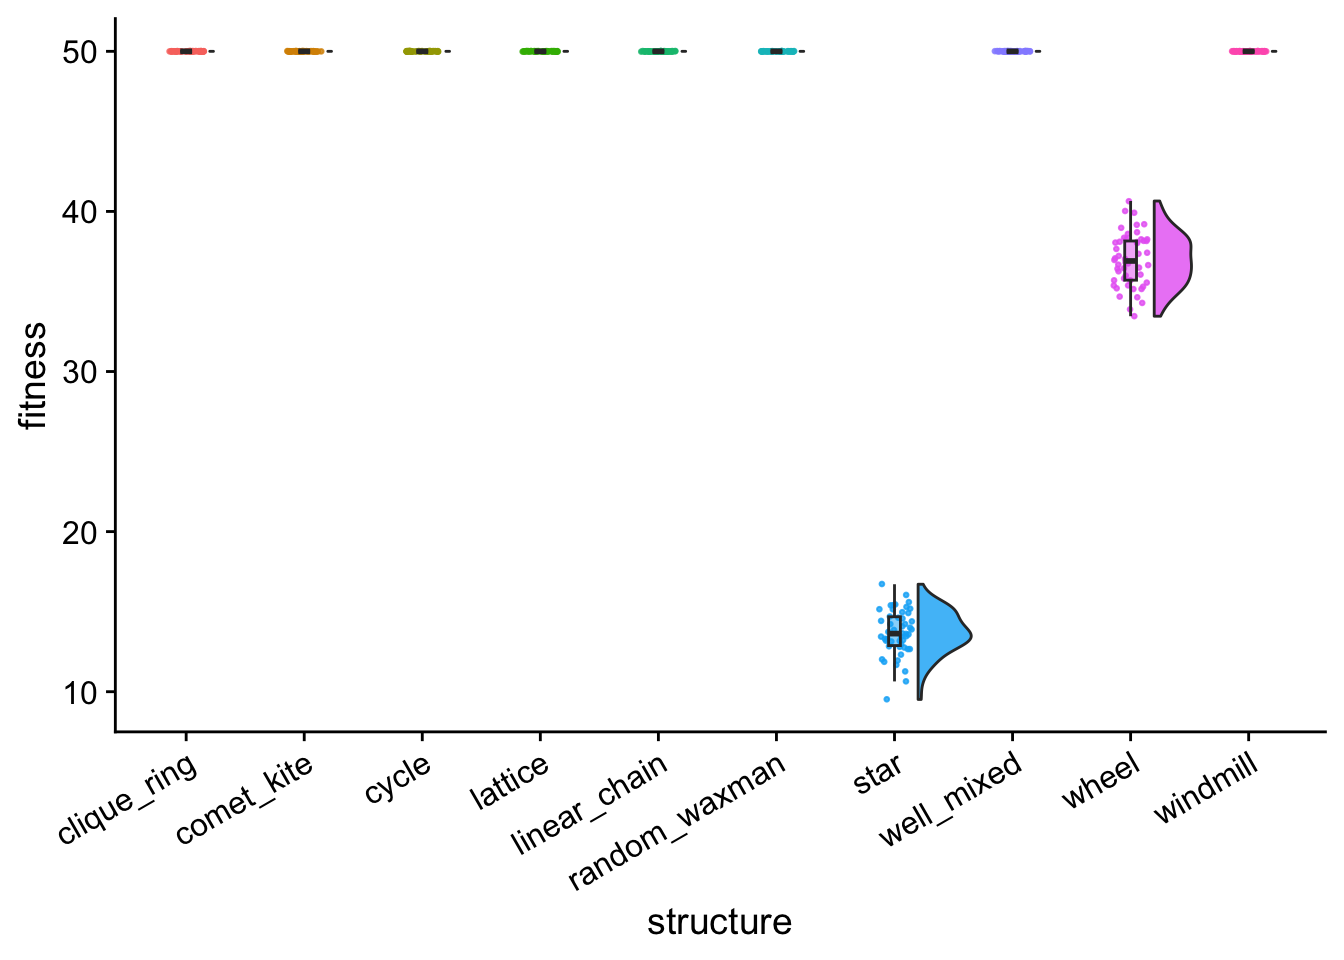
\includegraphics{supplemental-material_files/figure-latex/unnamed-chunk-8-1.pdf}

Maximum fitness over time

\begin{Shaded}
\begin{Highlighting}[]
\NormalTok{single\_gradient\_fitness\_ts\_plt }\OtherTok{\textless{}{-}} \FunctionTok{ggplot}\NormalTok{(}
    \AttributeTok{data =} \FunctionTok{filter}\NormalTok{(max\_org\_data\_ts, landscape }\SpecialCharTok{==} \StringTok{"Single gradient"}\NormalTok{),}
    \AttributeTok{mapping =} \FunctionTok{aes}\NormalTok{(}
      \AttributeTok{x =}\NormalTok{ generation,}
      \AttributeTok{y =}\NormalTok{ fitness,}
      \AttributeTok{color =}\NormalTok{ structure,}
      \AttributeTok{fill =}\NormalTok{ structure}
\NormalTok{    )}
\NormalTok{  ) }\SpecialCharTok{+}
  \FunctionTok{stat\_summary}\NormalTok{(}\AttributeTok{fun =} \StringTok{"mean"}\NormalTok{, }\AttributeTok{geom =} \StringTok{"line"}\NormalTok{) }\SpecialCharTok{+}
  \FunctionTok{stat\_summary}\NormalTok{(}
    \AttributeTok{fun.data =} \StringTok{"mean\_cl\_boot"}\NormalTok{,}
    \AttributeTok{fun.args =} \FunctionTok{list}\NormalTok{(}\AttributeTok{conf.int =} \FloatTok{0.95}\NormalTok{),}
    \AttributeTok{geom =} \StringTok{"ribbon"}\NormalTok{,}
    \AttributeTok{alpha =} \FloatTok{0.2}\NormalTok{,}
    \AttributeTok{linetype =} \DecValTok{0}
\NormalTok{  ) }\SpecialCharTok{+}
  \FunctionTok{theme}\NormalTok{(}\AttributeTok{legend.position =} \StringTok{"bottom"}\NormalTok{)}

\FunctionTok{ggsave}\NormalTok{(}
  \AttributeTok{plot =}\NormalTok{ single\_gradient\_fitness\_ts\_plt,}
  \AttributeTok{filename =} \FunctionTok{paste0}\NormalTok{(}
\NormalTok{    plot\_dir,}
    \StringTok{"/single\_gradient\_fitness\_ts.pdf"}
\NormalTok{  ),}
  \AttributeTok{width =} \DecValTok{15}\NormalTok{,}
  \AttributeTok{height =} \DecValTok{10}
\NormalTok{)}

\NormalTok{single\_gradient\_fitness\_ts\_plt}
\end{Highlighting}
\end{Shaded}

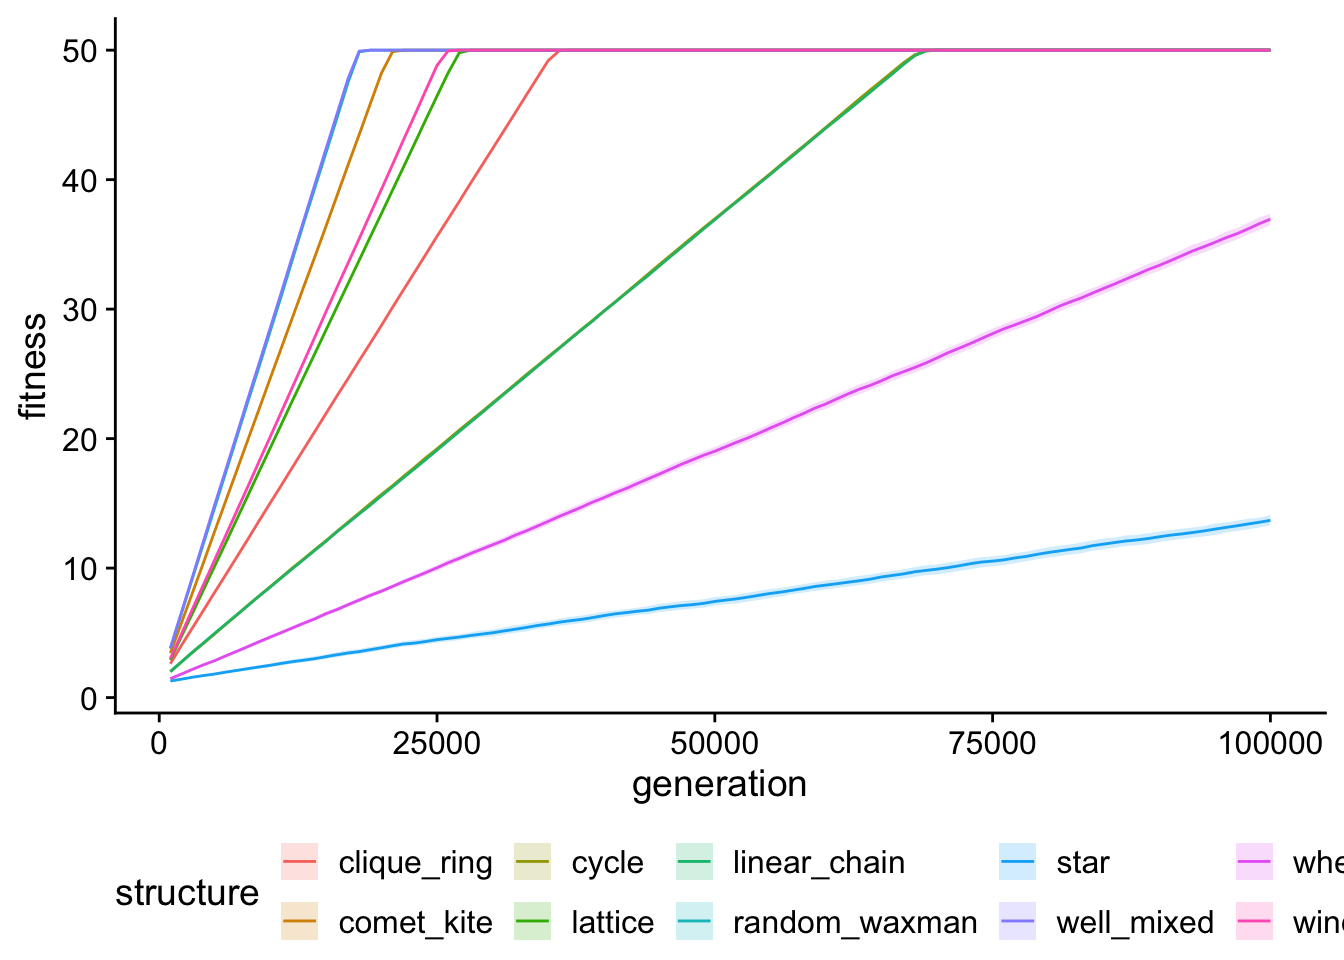
\includegraphics{supplemental-material_files/figure-latex/unnamed-chunk-9-1.pdf}

Time to maximum fitness

\begin{Shaded}
\begin{Highlighting}[]
\CommentTok{\# Find all rows with maximum fitness value, then get row with minimum generation,}
\CommentTok{\#  then project out expected generation to max (for runs that didn\textquotesingle{}t finish)}
\NormalTok{max\_possible\_fit }\OtherTok{=} \DecValTok{50}
\NormalTok{time\_to\_max\_single\_gradient }\OtherTok{\textless{}{-}}\NormalTok{ max\_org\_data\_ts }\SpecialCharTok{\%\textgreater{}\%}
  \FunctionTok{filter}\NormalTok{(landscape }\SpecialCharTok{==} \StringTok{"Single gradient"}\NormalTok{) }\SpecialCharTok{\%\textgreater{}\%}
  \FunctionTok{group\_by}\NormalTok{(rep, structure) }\SpecialCharTok{\%\textgreater{}\%}
  \FunctionTok{slice\_max}\NormalTok{(}
\NormalTok{    fitness,}
    \AttributeTok{n =} \DecValTok{1}
\NormalTok{  ) }\SpecialCharTok{\%\textgreater{}\%}
  \FunctionTok{slice\_min}\NormalTok{(}
\NormalTok{    generation,}
    \AttributeTok{n =} \DecValTok{1}
\NormalTok{  ) }\SpecialCharTok{\%\textgreater{}\%}
  \FunctionTok{mutate}\NormalTok{(}
    \AttributeTok{proj\_gen\_max =}\NormalTok{ (max\_possible\_fit }\SpecialCharTok{/}\NormalTok{ fitness) }\SpecialCharTok{*}\NormalTok{ generation}
\NormalTok{  )}
\end{Highlighting}
\end{Shaded}

\begin{Shaded}
\begin{Highlighting}[]
\NormalTok{single\_gradient\_gen\_max\_proj\_plt }\OtherTok{\textless{}{-}} \FunctionTok{ggplot}\NormalTok{(}
    \AttributeTok{data =}\NormalTok{ time\_to\_max\_single\_gradient,}
    \AttributeTok{mapping =} \FunctionTok{aes}\NormalTok{(}
      \AttributeTok{x =}\NormalTok{ structure,}
      \AttributeTok{y =}\NormalTok{ proj\_gen\_max,}
      \AttributeTok{fill =}\NormalTok{ structure}
\NormalTok{    )}
\NormalTok{  ) }\SpecialCharTok{+}
  \FunctionTok{geom\_flat\_violin}\NormalTok{(}
    \AttributeTok{position =} \FunctionTok{position\_nudge}\NormalTok{(}\AttributeTok{x =}\NormalTok{ .}\DecValTok{2}\NormalTok{, }\AttributeTok{y =} \DecValTok{0}\NormalTok{),}
    \AttributeTok{alpha =}\NormalTok{ .}\DecValTok{8}
\NormalTok{  ) }\SpecialCharTok{+}
  \FunctionTok{geom\_point}\NormalTok{(}
    \AttributeTok{mapping =} \FunctionTok{aes}\NormalTok{(}\AttributeTok{color =}\NormalTok{ structure),}
    \AttributeTok{position =} \FunctionTok{position\_jitter}\NormalTok{(}\AttributeTok{width =}\NormalTok{ .}\DecValTok{15}\NormalTok{),}
    \AttributeTok{size =}\NormalTok{ .}\DecValTok{5}\NormalTok{,}
    \AttributeTok{alpha =} \FloatTok{0.8}
\NormalTok{  ) }\SpecialCharTok{+}
  \FunctionTok{geom\_boxplot}\NormalTok{(}
    \AttributeTok{width =}\NormalTok{ .}\DecValTok{1}\NormalTok{,}
    \AttributeTok{outlier.shape =} \ConstantTok{NA}\NormalTok{,}
    \AttributeTok{alpha =} \FloatTok{0.5}
\NormalTok{  ) }\SpecialCharTok{+}
  \FunctionTok{scale\_y\_log10}\NormalTok{(}
    \AttributeTok{guide =} \StringTok{"axis\_logticks"}
\NormalTok{  ) }\SpecialCharTok{+}
  \CommentTok{\# scale\_y\_continuous(}
  \CommentTok{\#   trans="pseudo\_log",}
  \CommentTok{\#   breaks = c(10, 100, 1000, 10000, 100000, 1000000)}
  \CommentTok{\#   ,limits = c(10, 100, 1000, 10000, 100000, 1000000)}
  \CommentTok{\# ) +}
  \FunctionTok{geom\_hline}\NormalTok{(}
    \AttributeTok{yintercept =}\NormalTok{ max\_generation,}
    \AttributeTok{linetype =} \StringTok{"dashed"}
\NormalTok{  ) }\SpecialCharTok{+}
  \FunctionTok{theme}\NormalTok{(}
    \AttributeTok{legend.position =} \StringTok{"none"}\NormalTok{,}
    \AttributeTok{axis.text.x =} \FunctionTok{element\_text}\NormalTok{(}
      \AttributeTok{angle =} \DecValTok{30}\NormalTok{,}
      \AttributeTok{hjust =} \DecValTok{1}
\NormalTok{    )}
\NormalTok{  )}

\FunctionTok{ggsave}\NormalTok{(}
  \AttributeTok{filename =} \FunctionTok{paste0}\NormalTok{(plot\_dir, }\StringTok{"/single\_gradient\_gen\_max\_proj.pdf"}\NormalTok{),}
  \AttributeTok{plot =}\NormalTok{ single\_gradient\_gen\_max\_proj\_plt,}
  \AttributeTok{width =} \DecValTok{15}\NormalTok{,}
  \AttributeTok{height =} \DecValTok{10}
\NormalTok{)}

\NormalTok{single\_gradient\_gen\_max\_proj\_plt}
\end{Highlighting}
\end{Shaded}

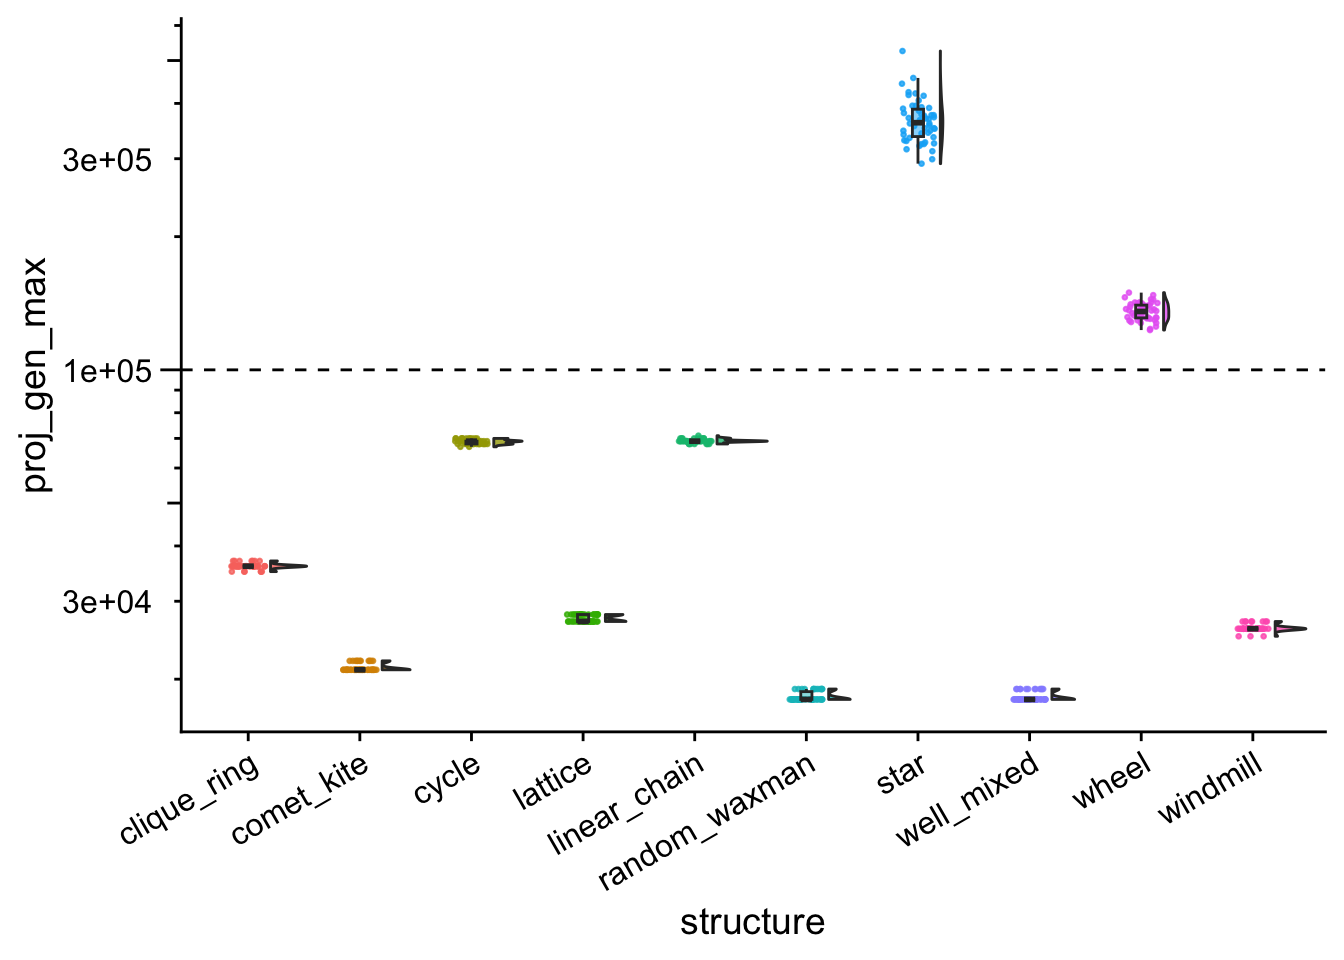
\includegraphics{supplemental-material_files/figure-latex/unnamed-chunk-11-1.pdf}

Rank ordering of time to max fitness values

\begin{Shaded}
\begin{Highlighting}[]
\NormalTok{time\_to\_max\_single\_gradient }\SpecialCharTok{\%\textgreater{}\%}
  \FunctionTok{group\_by}\NormalTok{(structure) }\SpecialCharTok{\%\textgreater{}\%}
  \FunctionTok{summarize}\NormalTok{(}
    \AttributeTok{reps =} \FunctionTok{n}\NormalTok{(),}
    \AttributeTok{median\_proj\_gen =} \FunctionTok{median}\NormalTok{(proj\_gen\_max),}
    \AttributeTok{mean\_proj\_gen =} \FunctionTok{mean}\NormalTok{(proj\_gen\_max)}
\NormalTok{  ) }\SpecialCharTok{\%\textgreater{}\%}
  \FunctionTok{arrange}\NormalTok{(}
\NormalTok{    mean\_proj\_gen}
\NormalTok{  )}
\end{Highlighting}
\end{Shaded}

\begin{verbatim}
## # A tibble: 10 x 4
##    structure      reps median_proj_gen mean_proj_gen
##    <fct>         <int>           <dbl>         <dbl>
##  1 well_mixed       50          18000         18240 
##  2 random_waxman    50          18000         18260 
##  3 comet_kite       50          21000         21220 
##  4 windmill         50          26000         26100 
##  5 lattice          50          27000         27460 
##  6 clique_ring      50          36000         36020 
##  7 cycle            50          69000         68840 
##  8 linear_chain     50          69000         69080 
##  9 wheel            50         135481.       135502.
## 10 star             50         361785.       366603.
\end{verbatim}

\begin{Shaded}
\begin{Highlighting}[]
\FunctionTok{kruskal.test}\NormalTok{(}
  \AttributeTok{formula =}\NormalTok{ proj\_gen\_max }\SpecialCharTok{\textasciitilde{}}\NormalTok{ structure,}
  \AttributeTok{data =}\NormalTok{ time\_to\_max\_single\_gradient}
\NormalTok{)}
\end{Highlighting}
\end{Shaded}

\begin{verbatim}
## 
##  Kruskal-Wallis rank sum test
## 
## data:  proj_gen_max by structure
## Kruskal-Wallis chi-squared = 490.93, df = 9, p-value < 2.2e-16
\end{verbatim}

\begin{Shaded}
\begin{Highlighting}[]
\NormalTok{wc\_results }\OtherTok{\textless{}{-}} \FunctionTok{pairwise.wilcox.test}\NormalTok{(}
  \AttributeTok{x =}\NormalTok{ time\_to\_max\_single\_gradient}\SpecialCharTok{$}\NormalTok{proj\_gen\_max,}
  \AttributeTok{g =}\NormalTok{ time\_to\_max\_single\_gradient}\SpecialCharTok{$}\NormalTok{structure,}
  \AttributeTok{p.adjust.method   =} \StringTok{"holm"}\NormalTok{,}
  \AttributeTok{exact =} \ConstantTok{FALSE}
\NormalTok{)}

\NormalTok{single\_gradient\_proj\_gen\_max\_wc\_table }\OtherTok{\textless{}{-}} \FunctionTok{kbl}\NormalTok{(wc\_results}\SpecialCharTok{$}\NormalTok{p.value) }\SpecialCharTok{\%\textgreater{}\%}
  \FunctionTok{kable\_styling}\NormalTok{()}

\FunctionTok{save\_kable}\NormalTok{(}
\NormalTok{  single\_gradient\_proj\_gen\_max\_wc\_table,}
  \FunctionTok{paste0}\NormalTok{(plot\_dir, }\StringTok{"/single\_gradient\_proj\_gen\_max\_wc\_table.pdf"}\NormalTok{)}
\NormalTok{)}

\NormalTok{single\_gradient\_proj\_gen\_max\_wc\_table}
\end{Highlighting}
\end{Shaded}

\begin{table}
\centering
\begin{tabular}[t]{l|r|r|r|r|r|r|r|r|r}
\hline
  & clique\_ring & comet\_kite & cycle & lattice & linear\_chain & random\_waxman & star & well\_mixed & wheel\\
\hline
comet\_kite & 0 & NA & NA & NA & NA & NA & NA & NA & NA\\
\hline
cycle & 0 & 0 & NA & NA & NA & NA & NA & NA & NA\\
\hline
lattice & 0 & 0 & 0.0000000 & NA & NA & NA & NA & NA & NA\\
\hline
linear\_chain & 0 & 0 & 0.2915242 & 0 & NA & NA & NA & NA & NA\\
\hline
random\_waxman & 0 & 0 & 0.0000000 & 0 & 0 & NA & NA & NA & NA\\
\hline
star & 0 & 0 & 0.0000000 & 0 & 0 & 0.0000000 & NA & NA & NA\\
\hline
well\_mixed & 0 & 0 & 0.0000000 & 0 & 0 & 0.8218339 & 0 & NA & NA\\
\hline
wheel & 0 & 0 & 0.0000000 & 0 & 0 & 0.0000000 & 0 & 0 & NA\\
\hline
windmill & 0 & 0 & 0.0000000 & 0 & 0 & 0.0000000 & 0 & 0 & 0\\
\hline
\end{tabular}
\end{table}

\begin{Shaded}
\begin{Highlighting}[]
\FunctionTok{library}\NormalTok{(boot)}
\CommentTok{\# Define sample mean function}
\NormalTok{samplemean }\OtherTok{\textless{}{-}} \ControlFlowTok{function}\NormalTok{(x, d) \{}
  \FunctionTok{return}\NormalTok{(}\FunctionTok{mean}\NormalTok{(x[d]))}
\NormalTok{\}}

\NormalTok{summary\_gen\_to\_max }\OtherTok{\textless{}{-}} \FunctionTok{tibble}\NormalTok{(}
  \AttributeTok{structure =} \FunctionTok{character}\NormalTok{(),}
  \AttributeTok{proj\_gen\_max\_mean =} \FunctionTok{double}\NormalTok{(),}
  \AttributeTok{proj\_gen\_max\_mean\_ci\_low =} \FunctionTok{double}\NormalTok{(),}
  \AttributeTok{proj\_gen\_max\_mean\_ci\_high =} \FunctionTok{double}\NormalTok{()}
\NormalTok{)}

\NormalTok{structures }\OtherTok{\textless{}{-}} \FunctionTok{levels}\NormalTok{(time\_to\_max\_single\_gradient}\SpecialCharTok{$}\NormalTok{structure)}
\ControlFlowTok{for}\NormalTok{ (struct }\ControlFlowTok{in}\NormalTok{ structures) \{}
\NormalTok{  boot\_result }\OtherTok{\textless{}{-}} \FunctionTok{boot}\NormalTok{(}
    \AttributeTok{data =} \FunctionTok{filter}\NormalTok{(}
\NormalTok{      time\_to\_max\_single\_gradient,}
\NormalTok{      structure }\SpecialCharTok{==}\NormalTok{ struct}
\NormalTok{    )}\SpecialCharTok{$}\NormalTok{proj\_gen\_max,}
    \AttributeTok{statistic =}\NormalTok{ samplemean,}
    \AttributeTok{R =} \DecValTok{10000}
\NormalTok{  )}
\NormalTok{  result\_ci }\OtherTok{\textless{}{-}} \FunctionTok{boot.ci}\NormalTok{(boot\_result, }\AttributeTok{conf =} \FloatTok{0.99}\NormalTok{, }\AttributeTok{type =} \StringTok{"perc"}\NormalTok{)}
\NormalTok{  m }\OtherTok{\textless{}{-}}\NormalTok{ result\_ci}\SpecialCharTok{$}\NormalTok{t0}
\NormalTok{  low }\OtherTok{\textless{}{-}}\NormalTok{ result\_ci}\SpecialCharTok{$}\NormalTok{percent[}\DecValTok{4}\NormalTok{]}
\NormalTok{  high }\OtherTok{\textless{}{-}}\NormalTok{ result\_ci}\SpecialCharTok{$}\NormalTok{percent[}\DecValTok{5}\NormalTok{]}

\NormalTok{  summary\_gen\_to\_max }\OtherTok{\textless{}{-}}\NormalTok{ summary\_gen\_to\_max }\SpecialCharTok{\%\textgreater{}\%}
    \FunctionTok{add\_row}\NormalTok{(}
      \AttributeTok{structure =}\NormalTok{ struct,}
      \AttributeTok{proj\_gen\_max\_mean =}\NormalTok{ m,}
      \AttributeTok{proj\_gen\_max\_mean\_ci\_low =}\NormalTok{ low,}
      \AttributeTok{proj\_gen\_max\_mean\_ci\_high =}\NormalTok{ high}
\NormalTok{    )}
\NormalTok{\}}

\NormalTok{wm\_median }\OtherTok{\textless{}{-}} \FunctionTok{median}\NormalTok{(}
  \FunctionTok{filter}\NormalTok{(time\_to\_max\_single\_gradient, structure }\SpecialCharTok{==} \StringTok{"well\_mixed"}\NormalTok{)}\SpecialCharTok{$}\NormalTok{proj\_gen\_max}
\NormalTok{)}

\NormalTok{simple\_time\_to\_max\_plt }\OtherTok{\textless{}{-}} \FunctionTok{ggplot}\NormalTok{(}
    \AttributeTok{data =}\NormalTok{ summary\_gen\_to\_max,}
    \AttributeTok{mapping =} \FunctionTok{aes}\NormalTok{(}
      \AttributeTok{x =}\NormalTok{ structure,}
      \AttributeTok{y =}\NormalTok{ proj\_gen\_max\_mean,}
      \AttributeTok{fill =}\NormalTok{ structure,}
      \AttributeTok{color =}\NormalTok{ structure}
\NormalTok{    )}
\NormalTok{  ) }\SpecialCharTok{+}
  \CommentTok{\# geom\_point() +}
  \FunctionTok{geom\_col}\NormalTok{() }\SpecialCharTok{+}
  \FunctionTok{geom\_linerange}\NormalTok{(}
    \FunctionTok{aes}\NormalTok{(}
      \AttributeTok{ymin =}\NormalTok{ proj\_gen\_max\_mean\_ci\_low,}
      \AttributeTok{ymax =}\NormalTok{ proj\_gen\_max\_mean\_ci\_high}
\NormalTok{    ),}
    \AttributeTok{color =} \StringTok{"black"}\NormalTok{,}
    \AttributeTok{linewidth =} \FloatTok{0.75}\NormalTok{,}
    \AttributeTok{lineend =} \StringTok{"round"}
\NormalTok{  ) }\SpecialCharTok{+}
  \CommentTok{\# scale\_y\_log10(}
  \CommentTok{\#   guide = "axis\_logticks"}
  \CommentTok{\# ) +}
  \FunctionTok{geom\_hline}\NormalTok{(}
    \AttributeTok{yintercept =}\NormalTok{ max\_generation,}
    \AttributeTok{linetype =} \StringTok{"dashed"}
\NormalTok{  ) }\SpecialCharTok{+}
  \FunctionTok{geom\_hline}\NormalTok{(}
    \AttributeTok{yintercept =}\NormalTok{ wm\_median,}
    \AttributeTok{linetype =} \StringTok{"dotted"}\NormalTok{,}
    \AttributeTok{color =} \StringTok{"orange"}
\NormalTok{  ) }\SpecialCharTok{+}
  \FunctionTok{scale\_color\_discreterainbow}\NormalTok{() }\SpecialCharTok{+}
  \FunctionTok{scale\_fill\_discreterainbow}\NormalTok{() }\SpecialCharTok{+}
  \FunctionTok{coord\_flip}\NormalTok{() }\SpecialCharTok{+}
  \FunctionTok{theme}\NormalTok{(}
    \AttributeTok{legend.position =} \StringTok{"none"}\NormalTok{,}
    \AttributeTok{axis.text.x =} \FunctionTok{element\_text}\NormalTok{(}
      \AttributeTok{angle =} \DecValTok{30}\NormalTok{,}
      \AttributeTok{hjust =} \DecValTok{1}
\NormalTok{    )}
\NormalTok{  )}

\FunctionTok{ggsave}\NormalTok{(}
  \AttributeTok{filename =} \FunctionTok{paste0}\NormalTok{(plot\_dir, }\StringTok{"/simple\_time\_to\_max.pdf"}\NormalTok{),}
  \AttributeTok{plot =}\NormalTok{ simple\_time\_to\_max\_plt,}
  \AttributeTok{width =} \DecValTok{8}\NormalTok{,}
  \AttributeTok{height =} \DecValTok{4}
\NormalTok{)}

\NormalTok{simple\_time\_to\_max\_plt}
\end{Highlighting}
\end{Shaded}

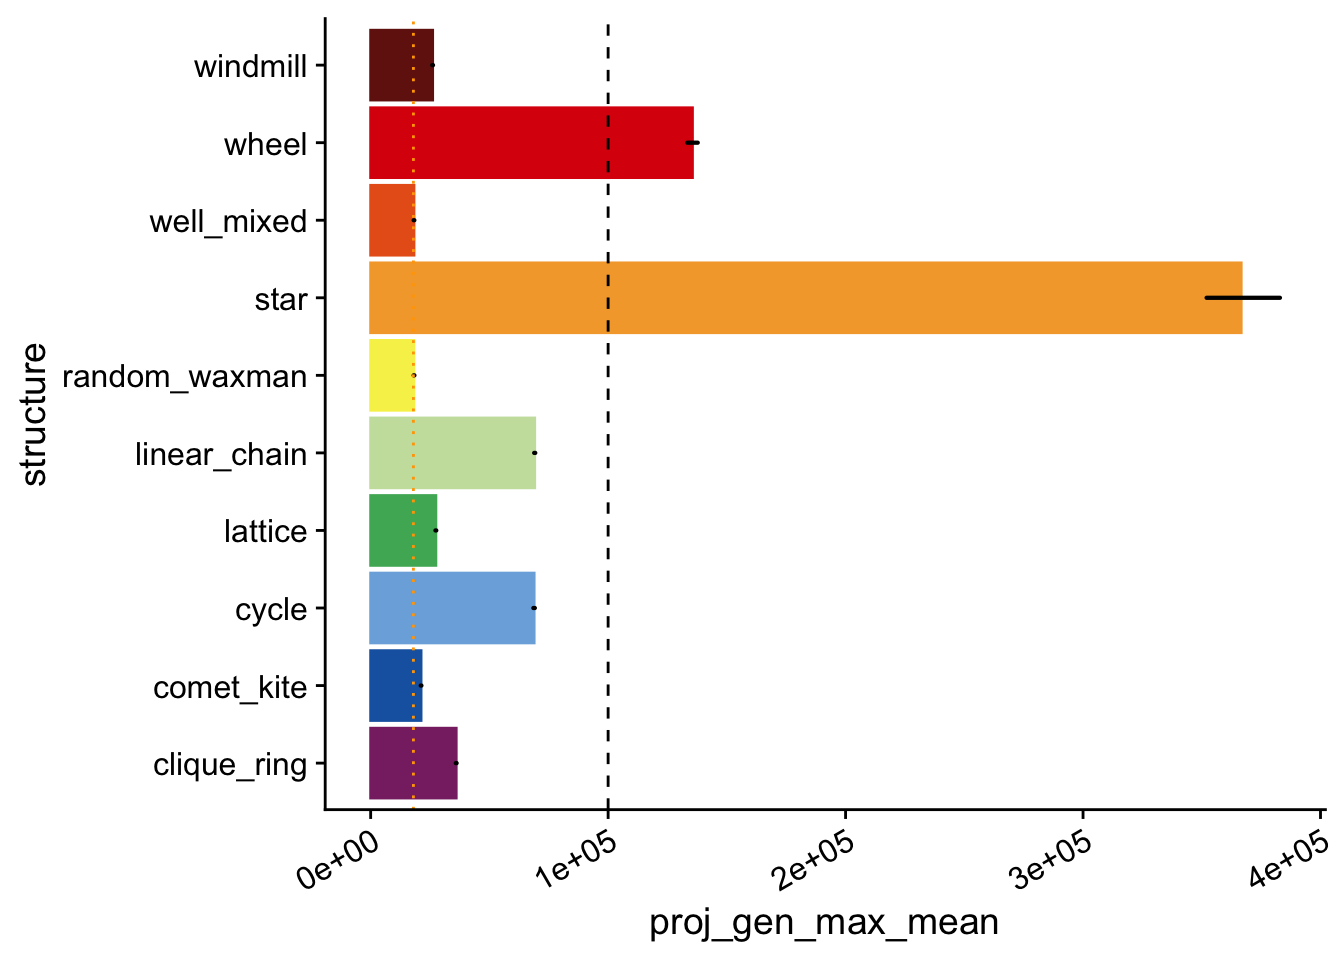
\includegraphics{supplemental-material_files/figure-latex/unnamed-chunk-14-1.pdf}

\hypertarget{fitness-in-multi-path-landscape}{%
\subsection{Fitness in multi-path landscape}\label{fitness-in-multi-path-landscape}}

\begin{Shaded}
\begin{Highlighting}[]
\NormalTok{multipath\_final\_fitness\_plt }\OtherTok{\textless{}{-}} \FunctionTok{ggplot}\NormalTok{(}
    \AttributeTok{data =} \FunctionTok{filter}\NormalTok{(max\_org\_data, landscape }\SpecialCharTok{==} \StringTok{"Multipath"}\NormalTok{),}
    \AttributeTok{mapping =} \FunctionTok{aes}\NormalTok{(}
      \AttributeTok{x =}\NormalTok{ structure,}
      \AttributeTok{y =}\NormalTok{ fitness,}
      \AttributeTok{fill =}\NormalTok{ structure}
\NormalTok{    )}
\NormalTok{  ) }\SpecialCharTok{+}
  \CommentTok{\# geom\_flat\_violin(}
  \CommentTok{\#   position = position\_nudge(x = .2, y = 0),}
  \CommentTok{\#   alpha = .8}
  \CommentTok{\# ) +}
  \FunctionTok{geom\_point}\NormalTok{(}
    \AttributeTok{mapping =} \FunctionTok{aes}\NormalTok{(}\AttributeTok{color =}\NormalTok{ structure),}
    \AttributeTok{position =} \FunctionTok{position\_jitter}\NormalTok{(}\AttributeTok{width =}\NormalTok{ .}\DecValTok{15}\NormalTok{),}
    \AttributeTok{size =}\NormalTok{ .}\DecValTok{5}\NormalTok{,}
    \AttributeTok{alpha =} \FloatTok{0.8}
\NormalTok{  ) }\SpecialCharTok{+}
  \FunctionTok{geom\_boxplot}\NormalTok{(}
    \AttributeTok{width =}\NormalTok{ .}\DecValTok{3}\NormalTok{,}
    \AttributeTok{outlier.shape =} \ConstantTok{NA}\NormalTok{,}
    \AttributeTok{alpha =} \FloatTok{0.5}
\NormalTok{  ) }\SpecialCharTok{+}
  \FunctionTok{scale\_color\_discreterainbow}\NormalTok{() }\SpecialCharTok{+}
  \FunctionTok{scale\_fill\_discreterainbow}\NormalTok{() }\SpecialCharTok{+}
  \FunctionTok{theme}\NormalTok{(}
    \AttributeTok{legend.position =} \StringTok{"none"}\NormalTok{,}
    \AttributeTok{axis.text.x =} \FunctionTok{element\_text}\NormalTok{(}
      \AttributeTok{angle =} \DecValTok{30}\NormalTok{,}
      \AttributeTok{hjust =} \DecValTok{1}
\NormalTok{    )}
\NormalTok{  )}

\FunctionTok{ggsave}\NormalTok{(}
  \AttributeTok{filename =} \FunctionTok{paste0}\NormalTok{(plot\_dir, }\StringTok{"/multipath\_final\_fitness.pdf"}\NormalTok{),}
  \AttributeTok{plot =}\NormalTok{ multipath\_final\_fitness\_plt,}
  \AttributeTok{width =} \DecValTok{6}\NormalTok{,}
  \AttributeTok{height =} \DecValTok{4}
\NormalTok{)}

\NormalTok{multipath\_final\_fitness\_plt}
\end{Highlighting}
\end{Shaded}

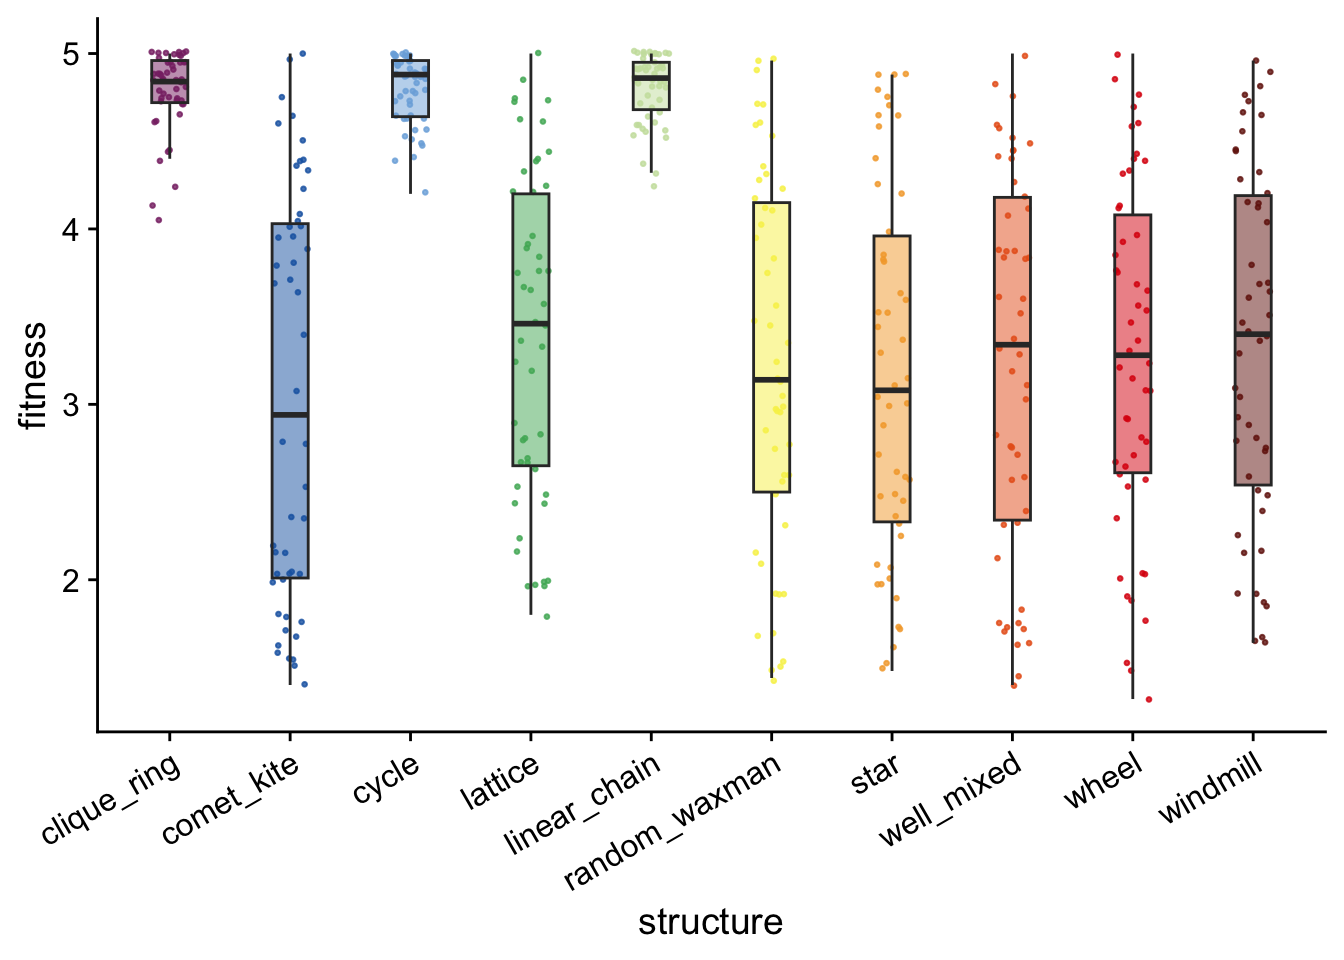
\includegraphics{supplemental-material_files/figure-latex/unnamed-chunk-15-1.pdf}

Max fitness over time

\begin{Shaded}
\begin{Highlighting}[]
\NormalTok{multipath\_fitness\_ts\_plt }\OtherTok{\textless{}{-}} \FunctionTok{ggplot}\NormalTok{(}
    \AttributeTok{data =} \FunctionTok{filter}\NormalTok{(max\_org\_data\_ts, landscape }\SpecialCharTok{==} \StringTok{"Multipath"}\NormalTok{),}
    \AttributeTok{mapping =} \FunctionTok{aes}\NormalTok{(}
      \AttributeTok{x =}\NormalTok{ generation,}
      \AttributeTok{y =}\NormalTok{ fitness,}
      \AttributeTok{color =}\NormalTok{ structure,}
      \AttributeTok{fill =}\NormalTok{ structure}
\NormalTok{    )}
\NormalTok{  ) }\SpecialCharTok{+}
  \FunctionTok{stat\_summary}\NormalTok{(}\AttributeTok{fun =} \StringTok{"mean"}\NormalTok{, }\AttributeTok{geom =} \StringTok{"line"}\NormalTok{) }\SpecialCharTok{+}
  \FunctionTok{stat\_summary}\NormalTok{(}
    \AttributeTok{fun.data =} \StringTok{"mean\_cl\_boot"}\NormalTok{,}
    \AttributeTok{fun.args =} \FunctionTok{list}\NormalTok{(}\AttributeTok{conf.int =} \FloatTok{0.95}\NormalTok{),}
    \AttributeTok{geom =} \StringTok{"ribbon"}\NormalTok{,}
    \AttributeTok{alpha =} \FloatTok{0.2}\NormalTok{,}
    \AttributeTok{linetype =} \DecValTok{0}
\NormalTok{  ) }\SpecialCharTok{+}
  \FunctionTok{theme}\NormalTok{(}\AttributeTok{legend.position =} \StringTok{"bottom"}\NormalTok{)}

\FunctionTok{ggsave}\NormalTok{(}
  \AttributeTok{plot =}\NormalTok{ multipath\_fitness\_ts\_plt,}
  \AttributeTok{filename =} \FunctionTok{paste0}\NormalTok{(}
\NormalTok{    plot\_dir,}
    \StringTok{"/multipath\_fitness\_ts.pdf"}
\NormalTok{  ),}
  \AttributeTok{width =} \DecValTok{15}\NormalTok{,}
  \AttributeTok{height =} \DecValTok{10}
\NormalTok{)}

\NormalTok{multipath\_fitness\_ts\_plt}
\end{Highlighting}
\end{Shaded}

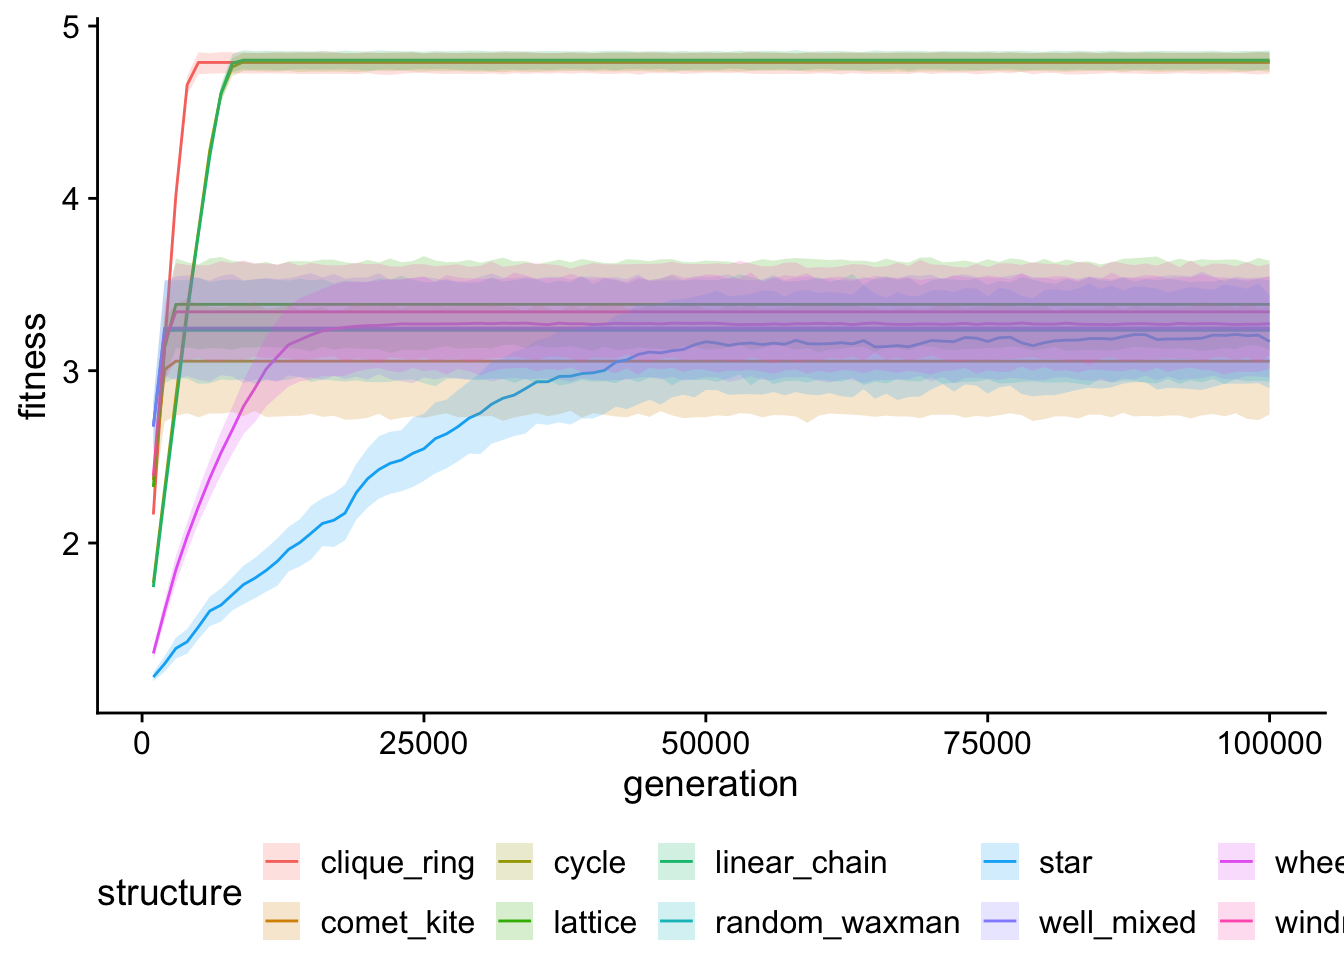
\includegraphics{supplemental-material_files/figure-latex/unnamed-chunk-16-1.pdf}

Rank ordering of fitness values

\begin{Shaded}
\begin{Highlighting}[]
\NormalTok{max\_org\_data }\SpecialCharTok{\%\textgreater{}\%}
  \FunctionTok{filter}\NormalTok{(landscape }\SpecialCharTok{==} \StringTok{"Multipath"}\NormalTok{) }\SpecialCharTok{\%\textgreater{}\%}
  \FunctionTok{group\_by}\NormalTok{(structure) }\SpecialCharTok{\%\textgreater{}\%}
  \FunctionTok{summarize}\NormalTok{(}
    \AttributeTok{reps =} \FunctionTok{n}\NormalTok{(),}
    \AttributeTok{median\_fitness =} \FunctionTok{median}\NormalTok{(fitness),}
    \AttributeTok{mean\_fitness =} \FunctionTok{mean}\NormalTok{(fitness)}
\NormalTok{  ) }\SpecialCharTok{\%\textgreater{}\%}
  \FunctionTok{arrange}\NormalTok{(}
    \FunctionTok{desc}\NormalTok{(mean\_fitness)}
\NormalTok{  )}
\end{Highlighting}
\end{Shaded}

\begin{verbatim}
## # A tibble: 10 x 4
##    structure      reps median_fitness mean_fitness
##    <fct>         <int>          <dbl>        <dbl>
##  1 linear_chain     50           4.86         4.80
##  2 cycle            50           4.88         4.79
##  3 clique_ring      50           4.84         4.79
##  4 lattice          50           3.46         3.38
##  5 windmill         50           3.4          3.34
##  6 wheel            50           3.28         3.27
##  7 well_mixed       50           3.34         3.25
##  8 random_waxman    50           3.14         3.23
##  9 star             50           3.08         3.17
## 10 comet_kite       50           2.94         3.06
\end{verbatim}

\begin{Shaded}
\begin{Highlighting}[]
\FunctionTok{kruskal.test}\NormalTok{(}
  \AttributeTok{formula =}\NormalTok{ fitness }\SpecialCharTok{\textasciitilde{}}\NormalTok{ structure,}
  \AttributeTok{data =} \FunctionTok{filter}\NormalTok{(max\_org\_data, landscape }\SpecialCharTok{==} \StringTok{"Multipath"}\NormalTok{)}
\NormalTok{)}
\end{Highlighting}
\end{Shaded}

\begin{verbatim}
## 
##  Kruskal-Wallis rank sum test
## 
## data:  fitness by structure
## Kruskal-Wallis chi-squared = 246.11, df = 9, p-value < 2.2e-16
\end{verbatim}

\begin{Shaded}
\begin{Highlighting}[]
\NormalTok{wc\_results }\OtherTok{\textless{}{-}} \FunctionTok{pairwise.wilcox.test}\NormalTok{(}
  \AttributeTok{x =} \FunctionTok{filter}\NormalTok{(max\_org\_data, landscape }\SpecialCharTok{==} \StringTok{"Multipath"}\NormalTok{)}\SpecialCharTok{$}\NormalTok{fitness,}
  \AttributeTok{g =} \FunctionTok{filter}\NormalTok{(max\_org\_data, landscape }\SpecialCharTok{==} \StringTok{"Multipath"}\NormalTok{)}\SpecialCharTok{$}\NormalTok{structure,}
  \AttributeTok{p.adjust.method   =} \StringTok{"holm"}\NormalTok{,}
  \AttributeTok{exact =} \ConstantTok{FALSE}
\NormalTok{)}

\NormalTok{mp\_fitness\_wc\_table }\OtherTok{\textless{}{-}} \FunctionTok{kbl}\NormalTok{(wc\_results}\SpecialCharTok{$}\NormalTok{p.value) }\SpecialCharTok{\%\textgreater{}\%}
  \FunctionTok{kable\_styling}\NormalTok{()}

\FunctionTok{save\_kable}\NormalTok{(}
\NormalTok{  mp\_fitness\_wc\_table,}
  \FunctionTok{paste0}\NormalTok{(plot\_dir, }\StringTok{"/multipath\_fitness\_wc\_table.pdf"}\NormalTok{)}
\NormalTok{)}

\NormalTok{mp\_fitness\_wc\_table}
\end{Highlighting}
\end{Shaded}

\begin{table}
\centering
\begin{tabular}[t]{l|r|r|r|r|r|r|r|r|r}
\hline
  & clique\_ring & comet\_kite & cycle & lattice & linear\_chain & random\_waxman & star & well\_mixed & wheel\\
\hline
comet\_kite & 0 & NA & NA & NA & NA & NA & NA & NA & NA\\
\hline
cycle & 1 & 0 & NA & NA & NA & NA & NA & NA & NA\\
\hline
lattice & 0 & 1 & 0 & NA & NA & NA & NA & NA & NA\\
\hline
linear\_chain & 1 & 0 & 1 & 0 & NA & NA & NA & NA & NA\\
\hline
random\_waxman & 0 & 1 & 0 & 1 & 0 & NA & NA & NA & NA\\
\hline
star & 0 & 1 & 0 & 1 & 0 & 1 & NA & NA & NA\\
\hline
well\_mixed & 0 & 1 & 0 & 1 & 0 & 1 & 1 & NA & NA\\
\hline
wheel & 0 & 1 & 0 & 1 & 0 & 1 & 1 & 1 & NA\\
\hline
windmill & 0 & 1 & 0 & 1 & 0 & 1 & 1 & 1 & 1\\
\hline
\end{tabular}
\end{table}

\hypertarget{valleys-crossed-in-valley-crossing-landscape}{%
\subsection{Valleys crossed in valley-crossing landscape}\label{valleys-crossed-in-valley-crossing-landscape}}

\begin{Shaded}
\begin{Highlighting}[]
\NormalTok{valleycrossing\_valleys\_plt }\OtherTok{\textless{}{-}} \FunctionTok{ggplot}\NormalTok{(}
    \AttributeTok{data =} \FunctionTok{filter}\NormalTok{(max\_org\_data, landscape }\SpecialCharTok{==} \StringTok{"Valley crossing"}\NormalTok{),}
    \AttributeTok{mapping =} \FunctionTok{aes}\NormalTok{(}
      \AttributeTok{x =}\NormalTok{ structure,}
      \AttributeTok{y =}\NormalTok{ valleys\_crossed,}
      \AttributeTok{fill =}\NormalTok{ structure}
\NormalTok{    )}
\NormalTok{  ) }\SpecialCharTok{+}
  \CommentTok{\# geom\_flat\_violin(}
  \CommentTok{\#   position = position\_nudge(x = .2, y = 0),}
  \CommentTok{\#   alpha = .8}
  \CommentTok{\# ) +}
  \FunctionTok{geom\_point}\NormalTok{(}
    \AttributeTok{mapping =} \FunctionTok{aes}\NormalTok{(}\AttributeTok{color =}\NormalTok{ structure),}
    \AttributeTok{position =} \FunctionTok{position\_jitter}\NormalTok{(}\AttributeTok{width =}\NormalTok{ .}\DecValTok{15}\NormalTok{),}
    \AttributeTok{size =}\NormalTok{ .}\DecValTok{5}\NormalTok{,}
    \AttributeTok{alpha =} \FloatTok{0.8}
\NormalTok{  ) }\SpecialCharTok{+}
  \FunctionTok{geom\_boxplot}\NormalTok{(}
    \AttributeTok{width =}\NormalTok{ .}\DecValTok{3}\NormalTok{,}
    \AttributeTok{outlier.shape =} \ConstantTok{NA}\NormalTok{,}
    \AttributeTok{alpha =} \FloatTok{0.5}
\NormalTok{  ) }\SpecialCharTok{+}
  \FunctionTok{scale\_color\_discreterainbow}\NormalTok{() }\SpecialCharTok{+}
  \FunctionTok{scale\_fill\_discreterainbow}\NormalTok{() }\SpecialCharTok{+}
  \FunctionTok{theme}\NormalTok{(}
    \AttributeTok{legend.position =} \StringTok{"none"}\NormalTok{,}
    \AttributeTok{axis.text.x =} \FunctionTok{element\_text}\NormalTok{(}
      \AttributeTok{angle =} \DecValTok{30}\NormalTok{,}
      \AttributeTok{hjust =} \DecValTok{1}
\NormalTok{    )}
\NormalTok{  )}

\FunctionTok{ggsave}\NormalTok{(}
  \AttributeTok{filename =} \FunctionTok{paste0}\NormalTok{(plot\_dir, }\StringTok{"/valleycrossing\_valleys\_crossed.pdf"}\NormalTok{),}
  \AttributeTok{plot =}\NormalTok{ valleycrossing\_valleys\_plt,}
  \AttributeTok{width =} \DecValTok{6}\NormalTok{,}
  \AttributeTok{height =} \DecValTok{4}
\NormalTok{)}

\NormalTok{valleycrossing\_valleys\_plt}
\end{Highlighting}
\end{Shaded}

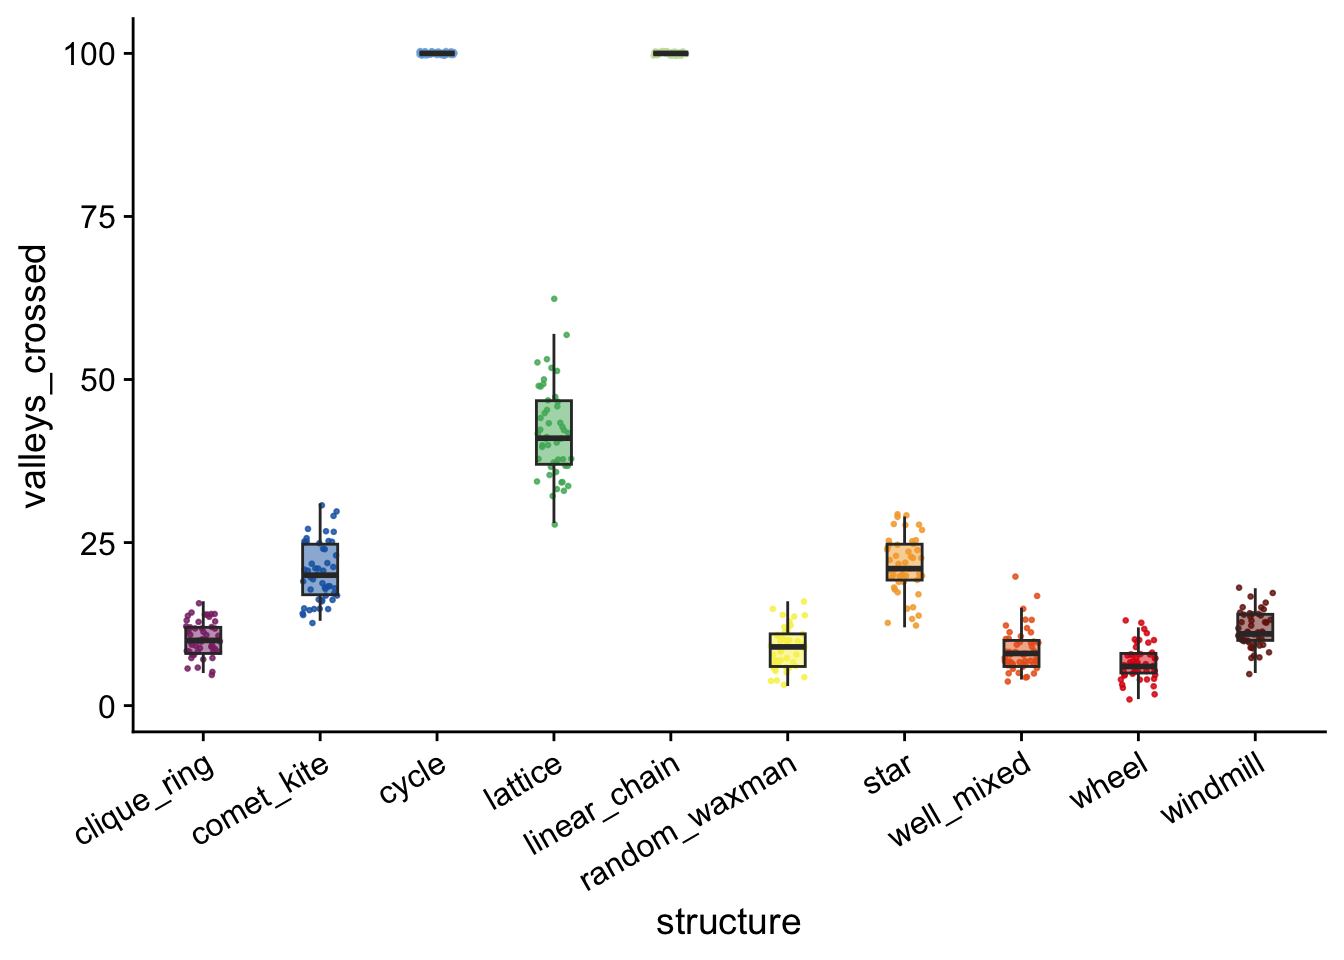
\includegraphics{supplemental-material_files/figure-latex/unnamed-chunk-19-1.pdf}

Rank ordering of fitness values

\begin{Shaded}
\begin{Highlighting}[]
\NormalTok{vc }\OtherTok{\textless{}{-}}\NormalTok{ max\_org\_data }\SpecialCharTok{\%\textgreater{}\%}
  \FunctionTok{filter}\NormalTok{(landscape }\SpecialCharTok{==} \StringTok{"Valley crossing"}\NormalTok{) }\SpecialCharTok{\%\textgreater{}\%}
  \FunctionTok{group\_by}\NormalTok{(structure) }\SpecialCharTok{\%\textgreater{}\%}
  \FunctionTok{summarize}\NormalTok{(}
    \AttributeTok{reps =} \FunctionTok{n}\NormalTok{(),}
    \AttributeTok{median\_valleys\_crossed =} \FunctionTok{median}\NormalTok{(valleys\_crossed),}
    \AttributeTok{mean\_valleys\_crossed =} \FunctionTok{mean}\NormalTok{(valleys\_crossed),}
    \AttributeTok{min\_valleys\_crossed =} \FunctionTok{min}\NormalTok{(valleys\_crossed)}
\NormalTok{  ) }\SpecialCharTok{\%\textgreater{}\%}
  \FunctionTok{arrange}\NormalTok{(}
    \FunctionTok{desc}\NormalTok{(mean\_valleys\_crossed)}
\NormalTok{  )}
\NormalTok{vc}
\end{Highlighting}
\end{Shaded}

\begin{verbatim}
## # A tibble: 10 x 5
##    structure      reps median_valleys_crossed mean_valleys_crossed
##    <fct>         <int>                  <dbl>                <dbl>
##  1 cycle            50                    100               100   
##  2 linear_chain     50                    100               100   
##  3 lattice          50                     41                41.9 
##  4 star             50                     21                21.5 
##  5 comet_kite       50                     20                20.5 
##  6 windmill         50                     11                11.6 
##  7 clique_ring      50                     10                10.3 
##  8 random_waxman    50                      9                 8.76
##  9 well_mixed       50                      8                 8.46
## 10 wheel            50                      6                 6.6 
## # i 1 more variable: min_valleys_crossed <dbl>
\end{verbatim}

\begin{Shaded}
\begin{Highlighting}[]
\NormalTok{vc}\SpecialCharTok{$}\NormalTok{min\_valleys\_crossed}
\end{Highlighting}
\end{Shaded}

\begin{verbatim}
##  [1] 100 100  28  12  13   5   5   3   4   1
\end{verbatim}

\begin{Shaded}
\begin{Highlighting}[]
\FunctionTok{kruskal.test}\NormalTok{(}
  \AttributeTok{formula =}\NormalTok{ valleys\_crossed }\SpecialCharTok{\textasciitilde{}}\NormalTok{ structure,}
  \AttributeTok{data =} \FunctionTok{filter}\NormalTok{(max\_org\_data, landscape }\SpecialCharTok{==} \StringTok{"Valley crossing"}\NormalTok{)}
\NormalTok{)}
\end{Highlighting}
\end{Shaded}

\begin{verbatim}
## 
##  Kruskal-Wallis rank sum test
## 
## data:  valleys_crossed by structure
## Kruskal-Wallis chi-squared = 444.04, df = 9, p-value < 2.2e-16
\end{verbatim}

\begin{Shaded}
\begin{Highlighting}[]
\NormalTok{wc\_results }\OtherTok{\textless{}{-}} \FunctionTok{pairwise.wilcox.test}\NormalTok{(}
  \AttributeTok{x =} \FunctionTok{filter}\NormalTok{(max\_org\_data, landscape }\SpecialCharTok{==} \StringTok{"Valley crossing"}\NormalTok{)}\SpecialCharTok{$}\NormalTok{valleys\_crossed,}
  \AttributeTok{g =} \FunctionTok{filter}\NormalTok{(max\_org\_data, landscape }\SpecialCharTok{==} \StringTok{"Valley crossing"}\NormalTok{)}\SpecialCharTok{$}\NormalTok{structure,}
  \AttributeTok{p.adjust.method   =} \StringTok{"holm"}\NormalTok{,}
  \AttributeTok{exact =} \ConstantTok{FALSE}
\NormalTok{)}

\NormalTok{vc\_valleys\_crossed\_wc\_table }\OtherTok{\textless{}{-}} \FunctionTok{kbl}\NormalTok{(wc\_results}\SpecialCharTok{$}\NormalTok{p.value) }\SpecialCharTok{\%\textgreater{}\%}
  \FunctionTok{kable\_styling}\NormalTok{()}

\FunctionTok{save\_kable}\NormalTok{(}
\NormalTok{  vc\_valleys\_crossed\_wc\_table,}
  \FunctionTok{paste0}\NormalTok{(plot\_dir, }\StringTok{"/valley\_crossing\_valleys\_wc\_table.pdf"}\NormalTok{)}
\NormalTok{)}

\NormalTok{vc\_valleys\_crossed\_wc\_table}
\end{Highlighting}
\end{Shaded}

\begin{table}
\centering
\begin{tabular}[t]{l|r|r|r|r|r|r|r|r|r}
\hline
  & clique\_ring & comet\_kite & cycle & lattice & linear\_chain & random\_waxman & star & well\_mixed & wheel\\
\hline
comet\_kite & 0.0000000 & NA & NA & NA & NA & NA & NA & NA & NA\\
\hline
cycle & 0.0000000 & 0.0000000 & NA & NA & NA & NA & NA & NA & NA\\
\hline
lattice & 0.0000000 & 0.0000000 & 0 & NA & NA & NA & NA & NA & NA\\
\hline
linear\_chain & 0.0000000 & 0.0000000 & NaN & 0 & NA & NA & NA & NA & NA\\
\hline
random\_waxman & 0.0414336 & 0.0000000 & 0 & 0 & 0 & NA & NA & NA & NA\\
\hline
star & 0.0000000 & 0.4016992 & 0 & 0 & 0 & 0.0000000 & NA & NA & NA\\
\hline
well\_mixed & 0.0028498 & 0.0000000 & 0 & 0 & 0 & 0.4620430 & 0 & NA & NA\\
\hline
wheel & 0.0000001 & 0.0000000 & 0 & 0 & 0 & 0.0029961 & 0 & 0.0119690 & NA\\
\hline
windmill & 0.0895493 & 0.0000000 & 0 & 0 & 0 & 0.0001323 & 0 & 0.0000028 & 0\\
\hline
\end{tabular}
\end{table}

\hypertarget{simple-model---squished-toroid-experiment-analyses}{%
\chapter{Simple model - Squished toroid experiment analyses}\label{simple-model---squished-toroid-experiment-analyses}}

\hypertarget{setup-and-dependencies}{%
\section{Setup and Dependencies}\label{setup-and-dependencies}}

\begin{Shaded}
\begin{Highlighting}[]
\FunctionTok{library}\NormalTok{(tidyverse)}
\FunctionTok{library}\NormalTok{(cowplot)}
\FunctionTok{library}\NormalTok{(RColorBrewer)}
\FunctionTok{library}\NormalTok{(khroma)}
\FunctionTok{library}\NormalTok{(rstatix)}
\FunctionTok{library}\NormalTok{(knitr)}
\FunctionTok{library}\NormalTok{(kableExtra)}
\FunctionTok{library}\NormalTok{(infer)}
\FunctionTok{source}\NormalTok{(}\StringTok{"https://gist.githubusercontent.com/benmarwick/2a1bb0133ff568cbe28d/raw/fb53bd97121f7f9ce947837ef1a4c65a73bffb3f/geom\_flat\_violin.R"}\NormalTok{)}
\end{Highlighting}
\end{Shaded}

\begin{Shaded}
\begin{Highlighting}[]
\CommentTok{\# Check if Rmd is being compiled using bookdown}
\NormalTok{bookdown }\OtherTok{\textless{}{-}} \FunctionTok{exists}\NormalTok{(}\StringTok{"bookdown\_build"}\NormalTok{)}
\end{Highlighting}
\end{Shaded}

\begin{Shaded}
\begin{Highlighting}[]
\NormalTok{experiment\_slug }\OtherTok{\textless{}{-}} \StringTok{"lattice{-}experiments"}
\NormalTok{working\_directory }\OtherTok{\textless{}{-}} \FunctionTok{paste}\NormalTok{(}
  \StringTok{"experiments"}\NormalTok{,}
  \StringTok{"mabe2{-}exps"}\NormalTok{,}
\NormalTok{  experiment\_slug,}
  \AttributeTok{sep =} \StringTok{"/"}
\NormalTok{)}
\CommentTok{\# Adjust working directory if being knitted for bookdown build.}
\ControlFlowTok{if}\NormalTok{ (bookdown) \{}
\NormalTok{  working\_directory }\OtherTok{\textless{}{-}} \FunctionTok{paste0}\NormalTok{(}
\NormalTok{    bookdown\_wd\_prefix,}
\NormalTok{    working\_directory}
\NormalTok{  )}
\NormalTok{\}}
\end{Highlighting}
\end{Shaded}

\begin{Shaded}
\begin{Highlighting}[]
\CommentTok{\# Configure our default graphing theme}
\FunctionTok{theme\_set}\NormalTok{(}\FunctionTok{theme\_cowplot}\NormalTok{())}
\CommentTok{\# Create a directory to store plots}
\NormalTok{plot\_dir }\OtherTok{\textless{}{-}} \FunctionTok{paste}\NormalTok{(}
\NormalTok{  working\_directory,}
  \StringTok{"rmd\_plots"}\NormalTok{,}
  \AttributeTok{sep =} \StringTok{"/"}
\NormalTok{)}

\FunctionTok{dir.create}\NormalTok{(}
\NormalTok{  plot\_dir,}
  \AttributeTok{showWarnings =} \ConstantTok{FALSE}
\NormalTok{)}
\end{Highlighting}
\end{Shaded}

\hypertarget{max-organism-data-analyses-1}{%
\section{Max organism data analyses}\label{max-organism-data-analyses-1}}

\begin{Shaded}
\begin{Highlighting}[]
\NormalTok{max\_generation }\OtherTok{\textless{}{-}} \DecValTok{100000}
\NormalTok{max\_org\_data\_path }\OtherTok{\textless{}{-}} \FunctionTok{paste}\NormalTok{(}
\NormalTok{  working\_directory,}
  \StringTok{"data"}\NormalTok{,}
  \StringTok{"combined\_max\_org\_data.csv"}\NormalTok{,}
  \AttributeTok{sep =} \StringTok{"/"}
\NormalTok{)}
\CommentTok{\# Data file has time series}
\NormalTok{max\_org\_data\_ts }\OtherTok{\textless{}{-}} \FunctionTok{read\_csv}\NormalTok{(max\_org\_data\_path)}
\NormalTok{max\_org\_data\_ts }\OtherTok{\textless{}{-}}\NormalTok{ max\_org\_data\_ts }\SpecialCharTok{\%\textgreater{}\%}
  \FunctionTok{mutate}\NormalTok{(}
    \AttributeTok{landscape =} \FunctionTok{as.factor}\NormalTok{(landscape),}
    \AttributeTok{structure =} \FunctionTok{factor}\NormalTok{(}
\NormalTok{      structure,}
      \AttributeTok{levels =} \FunctionTok{c}\NormalTok{(}
        \StringTok{"1\_3600"}\NormalTok{,}
        \StringTok{"2\_1800"}\NormalTok{,}
        \StringTok{"3\_1200"}\NormalTok{,}
        \StringTok{"4\_900"}\NormalTok{,}
        \StringTok{"15\_240"}\NormalTok{,}
        \StringTok{"30\_120"}\NormalTok{,}
        \StringTok{"60\_60"}
\NormalTok{      )}
\NormalTok{    ),}
\NormalTok{  ) }\SpecialCharTok{\%\textgreater{}\%}
  \FunctionTok{mutate}\NormalTok{(}
    \AttributeTok{valleys\_crossed =} \FunctionTok{case\_when}\NormalTok{(}
\NormalTok{      landscape }\SpecialCharTok{==} \StringTok{"Valley crossing"} \SpecialCharTok{\textasciitilde{}} \FunctionTok{round}\NormalTok{(}\FunctionTok{log}\NormalTok{(fitness, }\AttributeTok{base =} \FloatTok{1.5}\NormalTok{)),}
      \AttributeTok{.default =} \DecValTok{0}
\NormalTok{    )}
\NormalTok{  )}
\CommentTok{\# Get tibble with just final generation}
\NormalTok{max\_org\_data }\OtherTok{\textless{}{-}}\NormalTok{ max\_org\_data\_ts }\SpecialCharTok{\%\textgreater{}\%}
  \FunctionTok{filter}\NormalTok{(generation }\SpecialCharTok{==}\NormalTok{ max\_generation)}
\end{Highlighting}
\end{Shaded}

Check that replicate count for each condition matches expectations.

\begin{Shaded}
\begin{Highlighting}[]
\NormalTok{run\_summary }\OtherTok{\textless{}{-}}\NormalTok{ max\_org\_data }\SpecialCharTok{\%\textgreater{}\%}
  \FunctionTok{group\_by}\NormalTok{(landscape, structure) }\SpecialCharTok{\%\textgreater{}\%}
  \FunctionTok{summarize}\NormalTok{(}
    \AttributeTok{n =} \FunctionTok{n}\NormalTok{()}
\NormalTok{  )}
\FunctionTok{print}\NormalTok{(run\_summary, }\AttributeTok{n =} \DecValTok{30}\NormalTok{)}
\end{Highlighting}
\end{Shaded}

\begin{verbatim}
## # A tibble: 21 x 3
## # Groups:   landscape [3]
##    landscape       structure     n
##    <fct>           <fct>     <int>
##  1 Multipath       1_3600       50
##  2 Multipath       2_1800       50
##  3 Multipath       3_1200       50
##  4 Multipath       4_900        50
##  5 Multipath       15_240       50
##  6 Multipath       30_120       50
##  7 Multipath       60_60        50
##  8 Single gradient 1_3600       50
##  9 Single gradient 2_1800       50
## 10 Single gradient 3_1200       50
## 11 Single gradient 4_900        50
## 12 Single gradient 15_240       50
## 13 Single gradient 30_120       50
## 14 Single gradient 60_60        50
## 15 Valley crossing 1_3600       50
## 16 Valley crossing 2_1800       50
## 17 Valley crossing 3_1200       50
## 18 Valley crossing 4_900        50
## 19 Valley crossing 15_240       50
## 20 Valley crossing 30_120       50
## 21 Valley crossing 60_60        50
\end{verbatim}

\hypertarget{fitness-in-smooth-gradient-landscape-1}{%
\subsection{Fitness in smooth gradient landscape}\label{fitness-in-smooth-gradient-landscape-1}}

\begin{Shaded}
\begin{Highlighting}[]
\NormalTok{single\_gradient\_final\_fitness\_plt }\OtherTok{\textless{}{-}} \FunctionTok{ggplot}\NormalTok{(}
    \AttributeTok{data =} \FunctionTok{filter}\NormalTok{(max\_org\_data, landscape }\SpecialCharTok{==} \StringTok{"Single gradient"}\NormalTok{),}
    \AttributeTok{mapping =} \FunctionTok{aes}\NormalTok{(}
      \AttributeTok{x =}\NormalTok{ structure,}
      \AttributeTok{y =}\NormalTok{ fitness,}
      \AttributeTok{fill =}\NormalTok{ structure}
\NormalTok{    )}
\NormalTok{  ) }\SpecialCharTok{+}
  \FunctionTok{geom\_flat\_violin}\NormalTok{(}
    \AttributeTok{position =} \FunctionTok{position\_nudge}\NormalTok{(}\AttributeTok{x =}\NormalTok{ .}\DecValTok{2}\NormalTok{, }\AttributeTok{y =} \DecValTok{0}\NormalTok{),}
    \AttributeTok{alpha =}\NormalTok{ .}\DecValTok{8}
\NormalTok{  ) }\SpecialCharTok{+}
  \FunctionTok{geom\_point}\NormalTok{(}
    \AttributeTok{mapping =} \FunctionTok{aes}\NormalTok{(}\AttributeTok{color =}\NormalTok{ structure),}
    \AttributeTok{position =} \FunctionTok{position\_jitter}\NormalTok{(}\AttributeTok{width =}\NormalTok{ .}\DecValTok{15}\NormalTok{),}
    \AttributeTok{size =}\NormalTok{ .}\DecValTok{5}\NormalTok{,}
    \AttributeTok{alpha =} \FloatTok{0.8}
\NormalTok{  ) }\SpecialCharTok{+}
  \FunctionTok{geom\_boxplot}\NormalTok{(}
    \AttributeTok{width =}\NormalTok{ .}\DecValTok{1}\NormalTok{,}
    \AttributeTok{outlier.shape =} \ConstantTok{NA}\NormalTok{,}
    \AttributeTok{alpha =} \FloatTok{0.5}
\NormalTok{  ) }\SpecialCharTok{+}
  \FunctionTok{theme}\NormalTok{(}
    \AttributeTok{legend.position =} \StringTok{"none"}\NormalTok{,}
    \AttributeTok{axis.text.x =} \FunctionTok{element\_text}\NormalTok{(}
      \AttributeTok{angle =} \DecValTok{30}\NormalTok{,}
      \AttributeTok{hjust =} \DecValTok{1}
\NormalTok{    )}
\NormalTok{  )}

\FunctionTok{ggsave}\NormalTok{(}
  \AttributeTok{filename =} \FunctionTok{paste0}\NormalTok{(plot\_dir, }\StringTok{"/single\_gradient\_final\_fitness.pdf"}\NormalTok{),}
  \AttributeTok{plot =}\NormalTok{ single\_gradient\_final\_fitness\_plt,}
  \AttributeTok{width =} \DecValTok{15}\NormalTok{,}
  \AttributeTok{height =} \DecValTok{10}
\NormalTok{)}

\NormalTok{single\_gradient\_final\_fitness\_plt}
\end{Highlighting}
\end{Shaded}

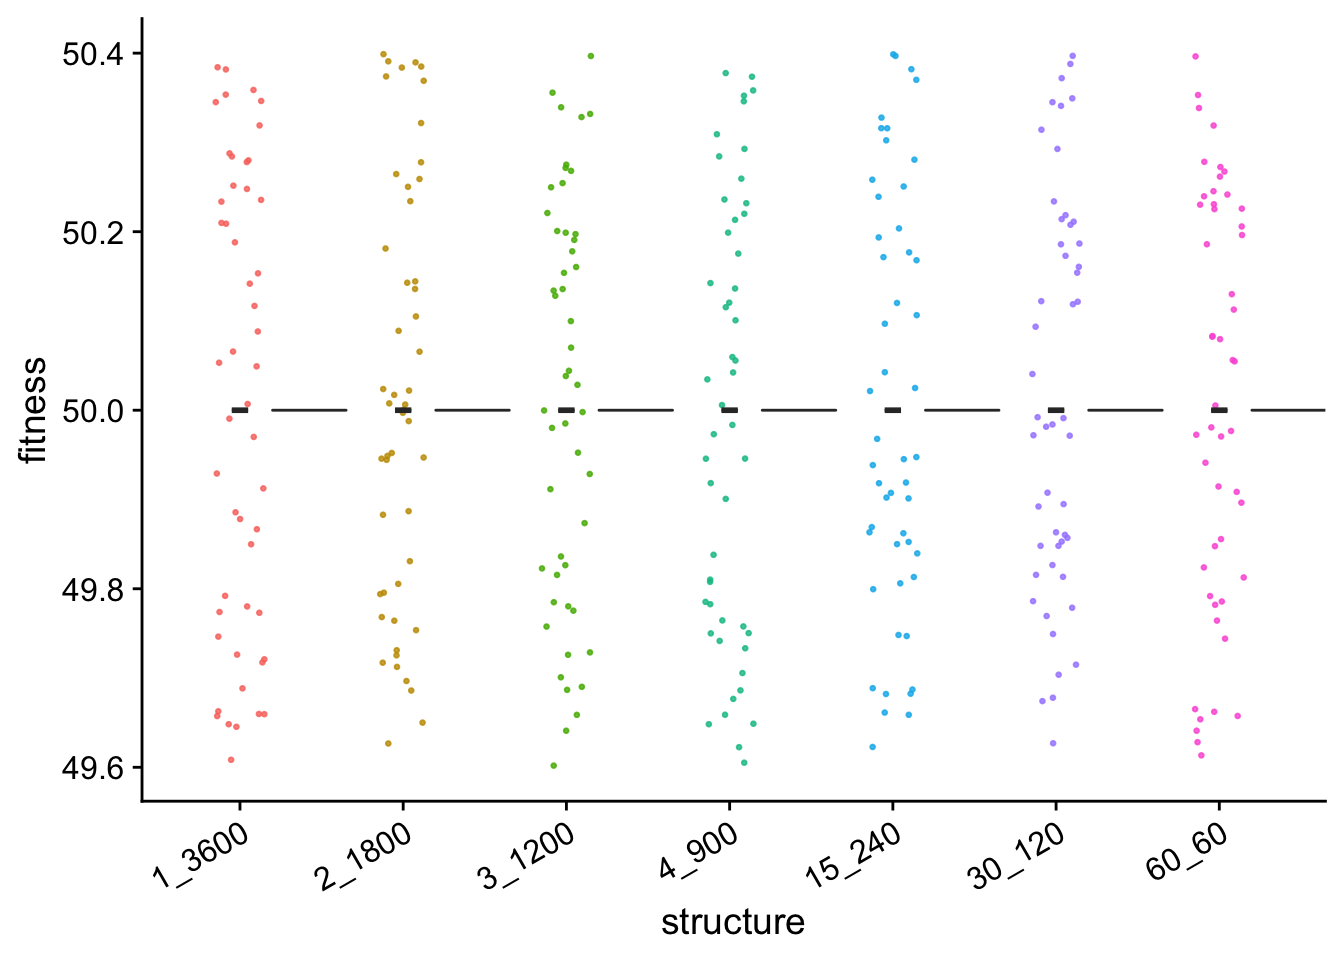
\includegraphics{supplemental-material_files/figure-latex/unnamed-chunk-28-1.pdf}

Max fitness over time

\begin{Shaded}
\begin{Highlighting}[]
\NormalTok{single\_gradient\_fitness\_ts\_plt }\OtherTok{\textless{}{-}} \FunctionTok{ggplot}\NormalTok{(}
    \AttributeTok{data =} \FunctionTok{filter}\NormalTok{(max\_org\_data\_ts, landscape }\SpecialCharTok{==} \StringTok{"Single gradient"}\NormalTok{),}
    \AttributeTok{mapping =} \FunctionTok{aes}\NormalTok{(}
      \AttributeTok{x =}\NormalTok{ generation,}
      \AttributeTok{y =}\NormalTok{ fitness,}
      \AttributeTok{color =}\NormalTok{ structure,}
      \AttributeTok{fill =}\NormalTok{ structure}
\NormalTok{    )}
\NormalTok{  ) }\SpecialCharTok{+}
  \FunctionTok{stat\_summary}\NormalTok{(}\AttributeTok{fun =} \StringTok{"mean"}\NormalTok{, }\AttributeTok{geom =} \StringTok{"line"}\NormalTok{) }\SpecialCharTok{+}
  \FunctionTok{stat\_summary}\NormalTok{(}
    \AttributeTok{fun.data =} \StringTok{"mean\_cl\_boot"}\NormalTok{,}
    \AttributeTok{fun.args =} \FunctionTok{list}\NormalTok{(}\AttributeTok{conf.int =} \FloatTok{0.95}\NormalTok{),}
    \AttributeTok{geom =} \StringTok{"ribbon"}\NormalTok{,}
    \AttributeTok{alpha =} \FloatTok{0.2}\NormalTok{,}
    \AttributeTok{linetype =} \DecValTok{0}
\NormalTok{  ) }\SpecialCharTok{+}
  \FunctionTok{theme}\NormalTok{(}\AttributeTok{legend.position =} \StringTok{"bottom"}\NormalTok{)}

\FunctionTok{ggsave}\NormalTok{(}
  \AttributeTok{plot =}\NormalTok{ single\_gradient\_fitness\_ts\_plt,}
  \AttributeTok{filename =} \FunctionTok{paste0}\NormalTok{(}
\NormalTok{    plot\_dir,}
    \StringTok{"/single\_gradient\_fitness\_ts.pdf"}
\NormalTok{  ),}
  \AttributeTok{width =} \DecValTok{15}\NormalTok{,}
  \AttributeTok{height =} \DecValTok{10}
\NormalTok{)}

\NormalTok{single\_gradient\_fitness\_ts\_plt}
\end{Highlighting}
\end{Shaded}

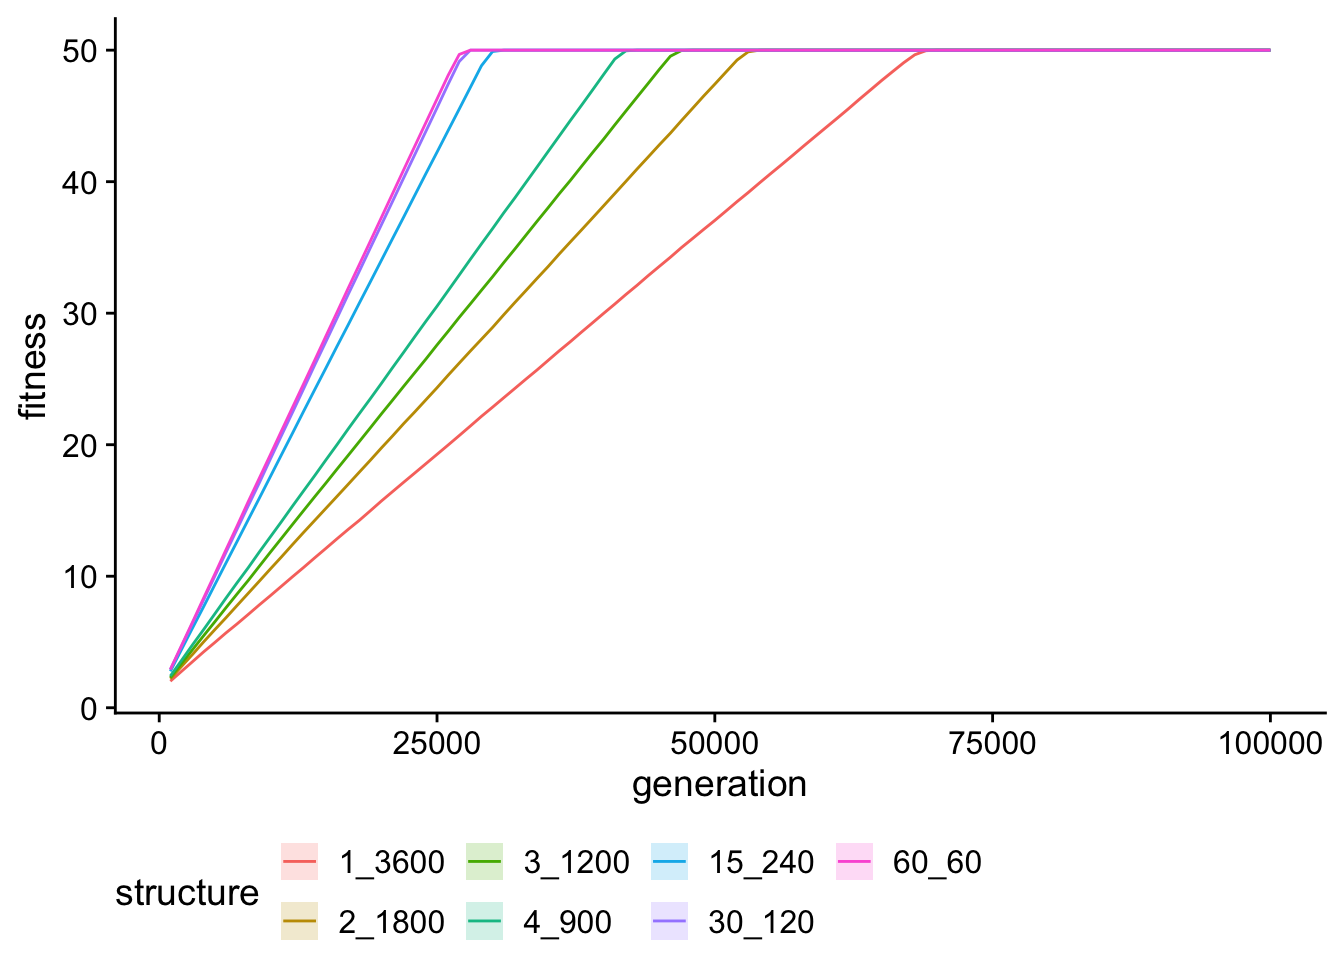
\includegraphics{supplemental-material_files/figure-latex/unnamed-chunk-29-1.pdf}

Time to maximum fitness

\begin{Shaded}
\begin{Highlighting}[]
\CommentTok{\# Find all rows with maximum fitness value, then get row with minimum generation,}
\CommentTok{\#  then project out expected generation to max (for runs that didn\textquotesingle{}t finish)}
\NormalTok{max\_possible\_fit }\OtherTok{=} \DecValTok{50}
\NormalTok{time\_to\_max\_single\_gradient }\OtherTok{\textless{}{-}}\NormalTok{ max\_org\_data\_ts }\SpecialCharTok{\%\textgreater{}\%}
  \FunctionTok{filter}\NormalTok{(landscape }\SpecialCharTok{==} \StringTok{"Single gradient"}\NormalTok{) }\SpecialCharTok{\%\textgreater{}\%}
  \FunctionTok{group\_by}\NormalTok{(rep, structure) }\SpecialCharTok{\%\textgreater{}\%}
  \FunctionTok{slice\_max}\NormalTok{(}
\NormalTok{    fitness,}
    \AttributeTok{n =} \DecValTok{1}
\NormalTok{  ) }\SpecialCharTok{\%\textgreater{}\%}
  \FunctionTok{slice\_min}\NormalTok{(}
\NormalTok{    generation,}
    \AttributeTok{n =} \DecValTok{1}
\NormalTok{  ) }\SpecialCharTok{\%\textgreater{}\%}
  \FunctionTok{mutate}\NormalTok{(}
    \AttributeTok{proj\_gen\_max =}\NormalTok{ (max\_possible\_fit }\SpecialCharTok{/}\NormalTok{ fitness) }\SpecialCharTok{*}\NormalTok{ generation}
\NormalTok{  )}
\end{Highlighting}
\end{Shaded}

\begin{Shaded}
\begin{Highlighting}[]
\NormalTok{single\_gradient\_gen\_max\_proj\_plt }\OtherTok{\textless{}{-}} \FunctionTok{ggplot}\NormalTok{(}
    \AttributeTok{data =}\NormalTok{ time\_to\_max\_single\_gradient,}
    \AttributeTok{mapping =} \FunctionTok{aes}\NormalTok{(}
      \AttributeTok{x =}\NormalTok{ structure,}
      \AttributeTok{y =}\NormalTok{ proj\_gen\_max,}
      \AttributeTok{fill =}\NormalTok{ structure}
\NormalTok{    )}
\NormalTok{  ) }\SpecialCharTok{+}
  \FunctionTok{geom\_flat\_violin}\NormalTok{(}
    \AttributeTok{position =} \FunctionTok{position\_nudge}\NormalTok{(}\AttributeTok{x =}\NormalTok{ .}\DecValTok{2}\NormalTok{, }\AttributeTok{y =} \DecValTok{0}\NormalTok{),}
    \AttributeTok{alpha =}\NormalTok{ .}\DecValTok{8}
\NormalTok{  ) }\SpecialCharTok{+}
  \FunctionTok{geom\_point}\NormalTok{(}
    \AttributeTok{mapping =} \FunctionTok{aes}\NormalTok{(}\AttributeTok{color =}\NormalTok{ structure),}
    \AttributeTok{position =} \FunctionTok{position\_jitter}\NormalTok{(}\AttributeTok{width =}\NormalTok{ .}\DecValTok{15}\NormalTok{),}
    \AttributeTok{size =}\NormalTok{ .}\DecValTok{5}\NormalTok{,}
    \AttributeTok{alpha =} \FloatTok{0.8}
\NormalTok{  ) }\SpecialCharTok{+}
  \FunctionTok{geom\_boxplot}\NormalTok{(}
    \AttributeTok{width =}\NormalTok{ .}\DecValTok{1}\NormalTok{,}
    \AttributeTok{outlier.shape =} \ConstantTok{NA}\NormalTok{,}
    \AttributeTok{alpha =} \FloatTok{0.5}
\NormalTok{  ) }\SpecialCharTok{+}
  \FunctionTok{scale\_y\_log10}\NormalTok{(}
    \AttributeTok{guide =} \StringTok{"axis\_logticks"}
\NormalTok{  ) }\SpecialCharTok{+}
  \CommentTok{\# scale\_y\_continuous(}
  \CommentTok{\#   trans="pseudo\_log",}
  \CommentTok{\#   breaks = c(10, 100, 1000, 10000, 100000, 1000000)}
  \CommentTok{\#   ,limits = c(10, 100, 1000, 10000, 100000, 1000000)}
  \CommentTok{\# ) +}
  \FunctionTok{geom\_hline}\NormalTok{(}
    \AttributeTok{yintercept =}\NormalTok{ max\_generation,}
    \AttributeTok{linetype =} \StringTok{"dashed"}
\NormalTok{  ) }\SpecialCharTok{+}
  \FunctionTok{theme}\NormalTok{(}
    \AttributeTok{legend.position =} \StringTok{"none"}\NormalTok{,}
    \AttributeTok{axis.text.x =} \FunctionTok{element\_text}\NormalTok{(}
      \AttributeTok{angle =} \DecValTok{30}\NormalTok{,}
      \AttributeTok{hjust =} \DecValTok{1}
\NormalTok{    )}
\NormalTok{  )}

\FunctionTok{ggsave}\NormalTok{(}
  \AttributeTok{filename =} \FunctionTok{paste0}\NormalTok{(plot\_dir, }\StringTok{"/single\_gradient\_gen\_max\_proj.pdf"}\NormalTok{),}
  \AttributeTok{plot =}\NormalTok{ single\_gradient\_gen\_max\_proj\_plt,}
  \AttributeTok{width =} \DecValTok{15}\NormalTok{,}
  \AttributeTok{height =} \DecValTok{10}
\NormalTok{)}

\NormalTok{single\_gradient\_gen\_max\_proj\_plt}
\end{Highlighting}
\end{Shaded}

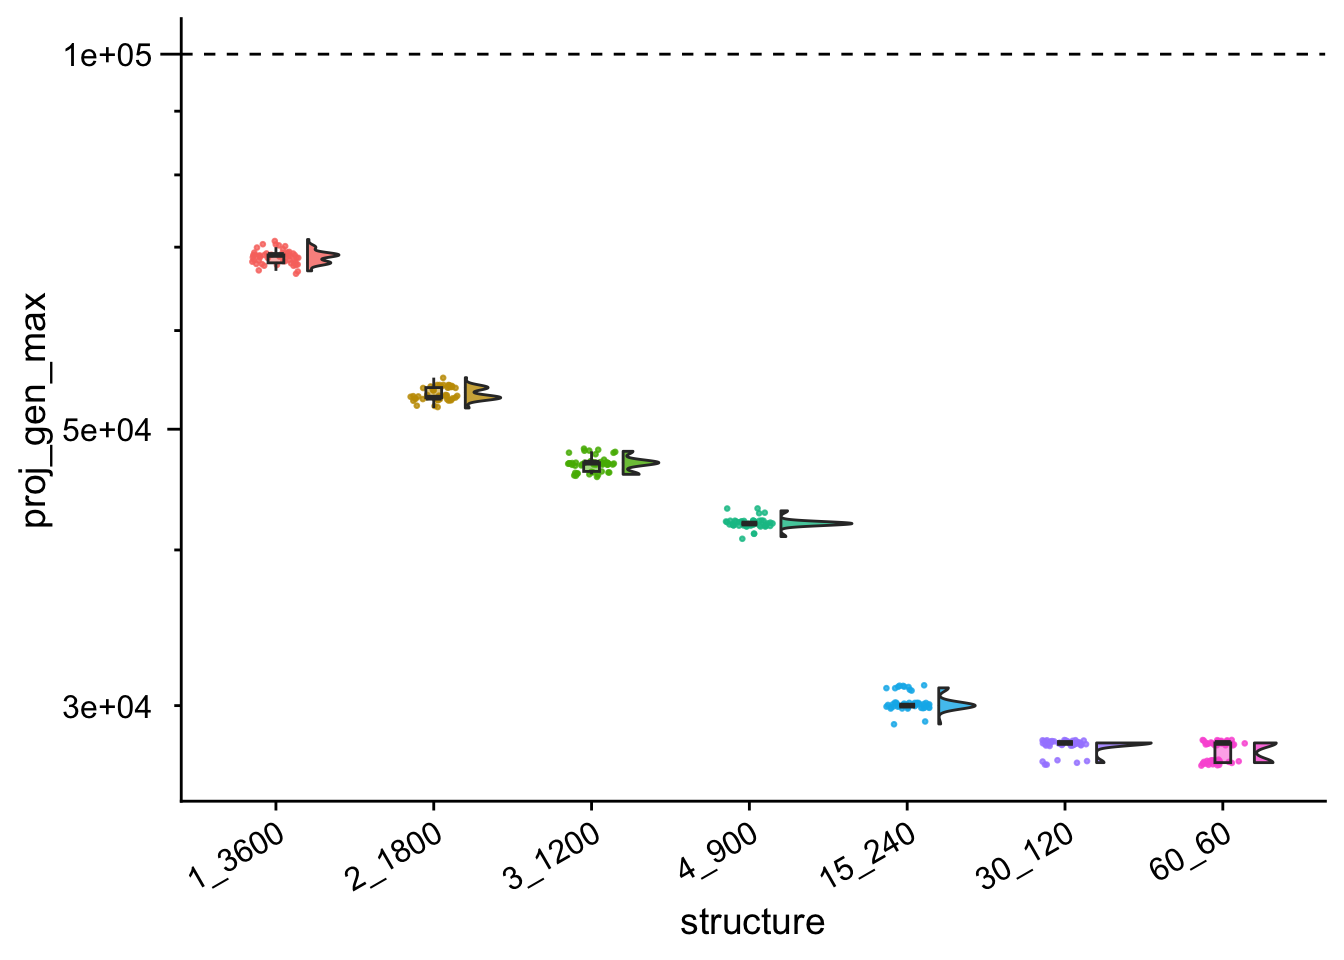
\includegraphics{supplemental-material_files/figure-latex/unnamed-chunk-31-1.pdf}

Rank ordering of time to max fitness values

\begin{Shaded}
\begin{Highlighting}[]
\NormalTok{time\_to\_max\_single\_gradient }\SpecialCharTok{\%\textgreater{}\%}
  \FunctionTok{group\_by}\NormalTok{(structure) }\SpecialCharTok{\%\textgreater{}\%}
  \FunctionTok{summarize}\NormalTok{(}
    \AttributeTok{reps =} \FunctionTok{n}\NormalTok{(),}
    \AttributeTok{median\_proj\_gen =} \FunctionTok{median}\NormalTok{(proj\_gen\_max),}
    \AttributeTok{mean\_proj\_gen =} \FunctionTok{mean}\NormalTok{(proj\_gen\_max)}
\NormalTok{  ) }\SpecialCharTok{\%\textgreater{}\%}
  \FunctionTok{arrange}\NormalTok{(}
\NormalTok{    mean\_proj\_gen}
\NormalTok{  )}
\end{Highlighting}
\end{Shaded}

\begin{verbatim}
## # A tibble: 7 x 4
##   structure  reps median_proj_gen mean_proj_gen
##   <fct>     <int>           <dbl>         <dbl>
## 1 60_60        50           28000         27540
## 2 30_120       50           28000         27880
## 3 15_240       50           30000         30160
## 4 4_900        50           42000         42020
## 5 3_1200       50           47000         46900
## 6 2_1800       50           53000         53340
## 7 1_3600       50           69000         68700
\end{verbatim}

\begin{Shaded}
\begin{Highlighting}[]
\FunctionTok{kruskal.test}\NormalTok{(}
  \AttributeTok{formula =}\NormalTok{ proj\_gen\_max }\SpecialCharTok{\textasciitilde{}}\NormalTok{ structure,}
  \AttributeTok{data =}\NormalTok{ time\_to\_max\_single\_gradient}
\NormalTok{)}
\end{Highlighting}
\end{Shaded}

\begin{verbatim}
## 
##  Kruskal-Wallis rank sum test
## 
## data:  proj_gen_max by structure
## Kruskal-Wallis chi-squared = 341.17, df = 6, p-value < 2.2e-16
\end{verbatim}

\begin{Shaded}
\begin{Highlighting}[]
\NormalTok{wc\_results }\OtherTok{\textless{}{-}} \FunctionTok{pairwise.wilcox.test}\NormalTok{(}
  \AttributeTok{x =}\NormalTok{ time\_to\_max\_single\_gradient}\SpecialCharTok{$}\NormalTok{proj\_gen\_max,}
  \AttributeTok{g =}\NormalTok{ time\_to\_max\_single\_gradient}\SpecialCharTok{$}\NormalTok{structure,}
  \AttributeTok{p.adjust.method   =} \StringTok{"holm"}\NormalTok{,}
  \AttributeTok{exact =} \ConstantTok{FALSE}
\NormalTok{)}

\NormalTok{single\_gradient\_proj\_gen\_max\_wc\_table }\OtherTok{\textless{}{-}} \FunctionTok{kbl}\NormalTok{(wc\_results}\SpecialCharTok{$}\NormalTok{p.value) }\SpecialCharTok{\%\textgreater{}\%}
  \FunctionTok{kable\_styling}\NormalTok{()}

\FunctionTok{save\_kable}\NormalTok{(}
\NormalTok{  single\_gradient\_proj\_gen\_max\_wc\_table,}
  \FunctionTok{paste0}\NormalTok{(plot\_dir, }\StringTok{"/single\_gradient\_proj\_gen\_max\_wc\_table.pdf"}\NormalTok{)}
\NormalTok{)}
\NormalTok{single\_gradient\_proj\_gen\_max\_wc\_table}
\end{Highlighting}
\end{Shaded}

\begin{table}
\centering
\begin{tabular}[t]{l|r|r|r|r|r|r}
\hline
  & 1\_3600 & 2\_1800 & 3\_1200 & 4\_900 & 15\_240 & 30\_120\\
\hline
2\_1800 & 0 & NA & NA & NA & NA & NA\\
\hline
3\_1200 & 0 & 0 & NA & NA & NA & NA\\
\hline
4\_900 & 0 & 0 & 0 & NA & NA & NA\\
\hline
15\_240 & 0 & 0 & 0 & 0 & NA & NA\\
\hline
30\_120 & 0 & 0 & 0 & 0 & 0 & NA\\
\hline
60\_60 & 0 & 0 & 0 & 0 & 0 & 0.0001966\\
\hline
\end{tabular}
\end{table}

\begin{Shaded}
\begin{Highlighting}[]
\FunctionTok{library}\NormalTok{(boot)}
\CommentTok{\# Define sample mean function}
\NormalTok{samplemean }\OtherTok{\textless{}{-}} \ControlFlowTok{function}\NormalTok{(x, d) \{}
  \FunctionTok{return}\NormalTok{(}\FunctionTok{mean}\NormalTok{(x[d]))}
\NormalTok{\}}

\NormalTok{summary\_gen\_to\_max }\OtherTok{\textless{}{-}} \FunctionTok{tibble}\NormalTok{(}
  \AttributeTok{structure =} \FunctionTok{character}\NormalTok{(),}
  \AttributeTok{proj\_gen\_max\_mean =} \FunctionTok{double}\NormalTok{(),}
  \AttributeTok{proj\_gen\_max\_mean\_ci\_low =} \FunctionTok{double}\NormalTok{(),}
  \AttributeTok{proj\_gen\_max\_mean\_ci\_high =} \FunctionTok{double}\NormalTok{()}
\NormalTok{)}

\NormalTok{structures }\OtherTok{\textless{}{-}} \FunctionTok{levels}\NormalTok{(time\_to\_max\_single\_gradient}\SpecialCharTok{$}\NormalTok{structure)}
\ControlFlowTok{for}\NormalTok{ (struct }\ControlFlowTok{in}\NormalTok{ structures) \{}
\NormalTok{  boot\_result }\OtherTok{\textless{}{-}} \FunctionTok{boot}\NormalTok{(}
    \AttributeTok{data =} \FunctionTok{filter}\NormalTok{(}
\NormalTok{      time\_to\_max\_single\_gradient,}
\NormalTok{      structure }\SpecialCharTok{==}\NormalTok{ struct}
\NormalTok{    )}\SpecialCharTok{$}\NormalTok{proj\_gen\_max,}
    \AttributeTok{statistic =}\NormalTok{ samplemean,}
    \AttributeTok{R =} \DecValTok{10000}
\NormalTok{  )}
\NormalTok{  result\_ci }\OtherTok{\textless{}{-}} \FunctionTok{boot.ci}\NormalTok{(boot\_result, }\AttributeTok{conf =} \FloatTok{0.99}\NormalTok{, }\AttributeTok{type =} \StringTok{"perc"}\NormalTok{)}
\NormalTok{  m }\OtherTok{\textless{}{-}}\NormalTok{ result\_ci}\SpecialCharTok{$}\NormalTok{t0}
\NormalTok{  low }\OtherTok{\textless{}{-}}\NormalTok{ result\_ci}\SpecialCharTok{$}\NormalTok{percent[}\DecValTok{4}\NormalTok{]}
\NormalTok{  high }\OtherTok{\textless{}{-}}\NormalTok{ result\_ci}\SpecialCharTok{$}\NormalTok{percent[}\DecValTok{5}\NormalTok{]}

\NormalTok{  summary\_gen\_to\_max }\OtherTok{\textless{}{-}}\NormalTok{ summary\_gen\_to\_max }\SpecialCharTok{\%\textgreater{}\%}
    \FunctionTok{add\_row}\NormalTok{(}
      \AttributeTok{structure =}\NormalTok{ struct,}
      \AttributeTok{proj\_gen\_max\_mean =}\NormalTok{ m,}
      \AttributeTok{proj\_gen\_max\_mean\_ci\_low =}\NormalTok{ low,}
      \AttributeTok{proj\_gen\_max\_mean\_ci\_high =}\NormalTok{ high}
\NormalTok{    )}
\NormalTok{\}}

\NormalTok{wm\_median }\OtherTok{\textless{}{-}} \FunctionTok{median}\NormalTok{(}
  \FunctionTok{filter}\NormalTok{(time\_to\_max\_single\_gradient, structure }\SpecialCharTok{==} \StringTok{"well\_mixed"}\NormalTok{)}\SpecialCharTok{$}\NormalTok{proj\_gen\_max}
\NormalTok{)}

\NormalTok{simple\_time\_to\_max\_plt }\OtherTok{\textless{}{-}} \FunctionTok{ggplot}\NormalTok{(}
    \AttributeTok{data =}\NormalTok{ summary\_gen\_to\_max,}
    \AttributeTok{mapping =} \FunctionTok{aes}\NormalTok{(}
      \AttributeTok{x =}\NormalTok{ structure,}
      \AttributeTok{y =}\NormalTok{ proj\_gen\_max\_mean,}
      \AttributeTok{fill =}\NormalTok{ structure,}
      \AttributeTok{color =}\NormalTok{ structure}
\NormalTok{    )}
\NormalTok{  ) }\SpecialCharTok{+}
  \CommentTok{\# geom\_point() +}
  \FunctionTok{geom\_col}\NormalTok{() }\SpecialCharTok{+}
  \FunctionTok{geom\_linerange}\NormalTok{(}
    \FunctionTok{aes}\NormalTok{(}
      \AttributeTok{ymin =}\NormalTok{ proj\_gen\_max\_mean\_ci\_low,}
      \AttributeTok{ymax =}\NormalTok{ proj\_gen\_max\_mean\_ci\_high}
\NormalTok{    ),}
    \AttributeTok{color =} \StringTok{"black"}\NormalTok{,}
    \AttributeTok{linewidth =} \FloatTok{0.75}\NormalTok{,}
    \AttributeTok{lineend =} \StringTok{"round"}
\NormalTok{  ) }\SpecialCharTok{+}
  \CommentTok{\# scale\_y\_log10(}
  \CommentTok{\#   guide = "axis\_logticks"}
  \CommentTok{\# ) +}
  \FunctionTok{geom\_hline}\NormalTok{(}
    \AttributeTok{yintercept =}\NormalTok{ max\_generation,}
    \AttributeTok{linetype =} \StringTok{"dashed"}
\NormalTok{  ) }\SpecialCharTok{+}
  \FunctionTok{geom\_hline}\NormalTok{(}
    \AttributeTok{yintercept =}\NormalTok{ wm\_median,}
    \AttributeTok{linetype =} \StringTok{"dotted"}\NormalTok{,}
    \AttributeTok{color =} \StringTok{"orange"}
\NormalTok{  ) }\SpecialCharTok{+}
  \FunctionTok{scale\_color\_discreterainbow}\NormalTok{() }\SpecialCharTok{+}
  \FunctionTok{scale\_fill\_discreterainbow}\NormalTok{() }\SpecialCharTok{+}
  \FunctionTok{coord\_flip}\NormalTok{() }\SpecialCharTok{+}
  \FunctionTok{theme}\NormalTok{(}
    \AttributeTok{legend.position =} \StringTok{"none"}\NormalTok{,}
    \AttributeTok{axis.text.x =} \FunctionTok{element\_text}\NormalTok{(}
      \AttributeTok{angle =} \DecValTok{30}\NormalTok{,}
      \AttributeTok{hjust =} \DecValTok{1}
\NormalTok{    )}
\NormalTok{  )}

\FunctionTok{ggsave}\NormalTok{(}
  \AttributeTok{filename =} \FunctionTok{paste0}\NormalTok{(plot\_dir, }\StringTok{"/simple\_time\_to\_max.pdf"}\NormalTok{),}
  \AttributeTok{plot =}\NormalTok{ simple\_time\_to\_max\_plt,}
  \AttributeTok{width =} \DecValTok{8}\NormalTok{,}
  \AttributeTok{height =} \DecValTok{4}
\NormalTok{)}

\NormalTok{simple\_time\_to\_max\_plt}
\end{Highlighting}
\end{Shaded}

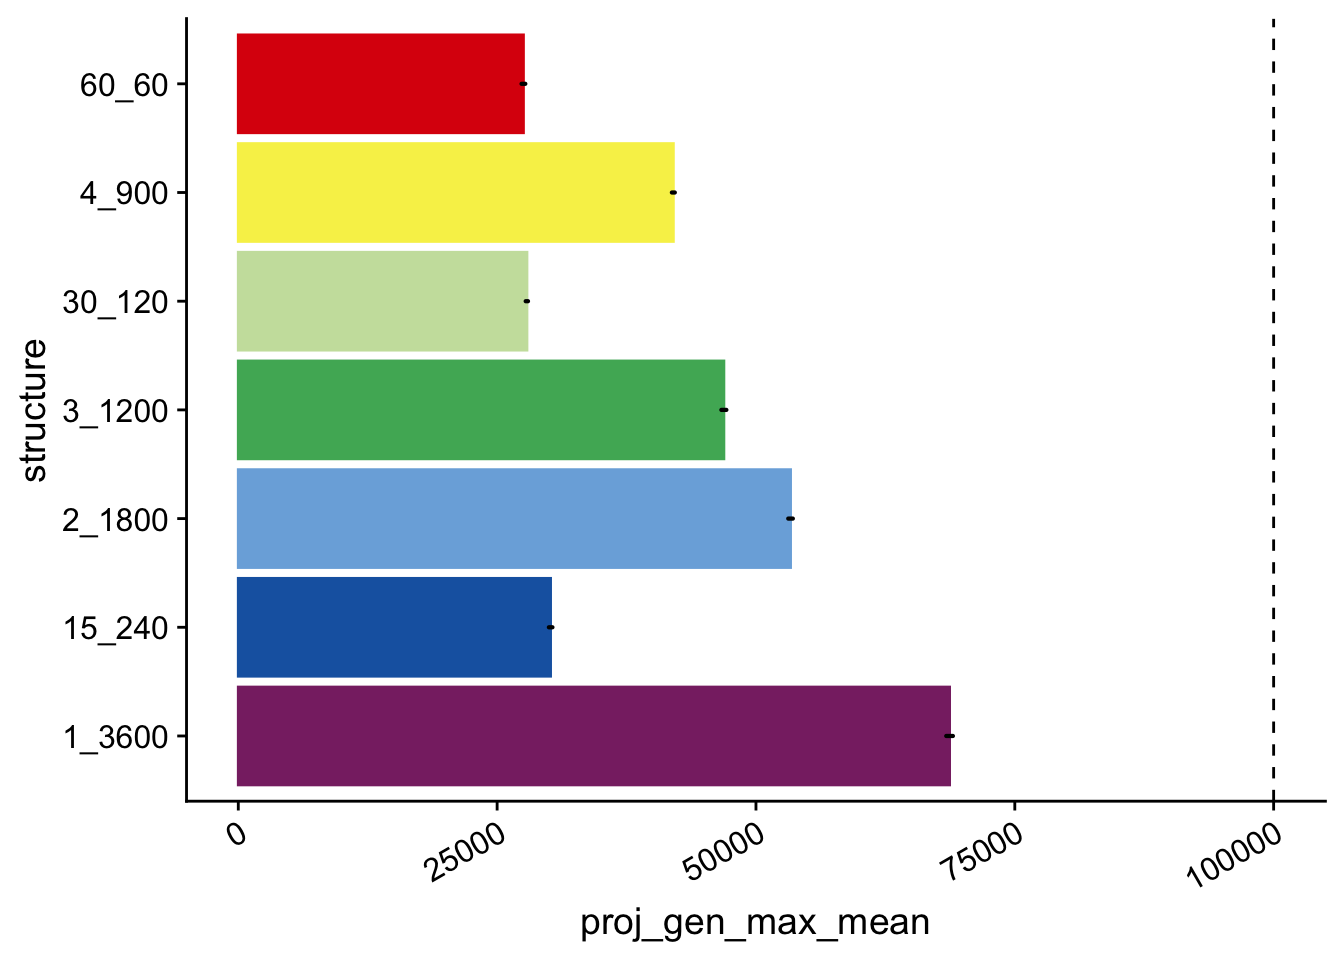
\includegraphics{supplemental-material_files/figure-latex/unnamed-chunk-34-1.pdf}

\hypertarget{fitness-in-multi-path-landscape-1}{%
\subsection{Fitness in multi-path landscape}\label{fitness-in-multi-path-landscape-1}}

\begin{Shaded}
\begin{Highlighting}[]
\NormalTok{multipath\_final\_fitness\_plt }\OtherTok{\textless{}{-}} \FunctionTok{ggplot}\NormalTok{(}
    \AttributeTok{data =} \FunctionTok{filter}\NormalTok{(max\_org\_data, landscape }\SpecialCharTok{==} \StringTok{"Multipath"}\NormalTok{),}
    \AttributeTok{mapping =} \FunctionTok{aes}\NormalTok{(}
      \AttributeTok{x =}\NormalTok{ structure,}
      \AttributeTok{y =}\NormalTok{ fitness,}
      \AttributeTok{fill =}\NormalTok{ structure}
\NormalTok{    )}
\NormalTok{  ) }\SpecialCharTok{+}
  \CommentTok{\# geom\_flat\_violin(}
  \CommentTok{\#   position = position\_nudge(x = .2, y = 0),}
  \CommentTok{\#   alpha = .8}
  \CommentTok{\# ) +}
  \FunctionTok{geom\_point}\NormalTok{(}
    \AttributeTok{mapping =} \FunctionTok{aes}\NormalTok{(}\AttributeTok{color =}\NormalTok{ structure),}
    \AttributeTok{position =} \FunctionTok{position\_jitter}\NormalTok{(}\AttributeTok{width =}\NormalTok{ .}\DecValTok{15}\NormalTok{),}
    \AttributeTok{size =}\NormalTok{ .}\DecValTok{5}\NormalTok{,}
    \AttributeTok{alpha =} \FloatTok{0.8}
\NormalTok{  ) }\SpecialCharTok{+}
  \FunctionTok{geom\_boxplot}\NormalTok{(}
    \AttributeTok{width =}\NormalTok{ .}\DecValTok{3}\NormalTok{,}
    \AttributeTok{outlier.shape =} \ConstantTok{NA}\NormalTok{,}
    \AttributeTok{alpha =} \FloatTok{0.5}
\NormalTok{  ) }\SpecialCharTok{+}
  \FunctionTok{scale\_color\_discreterainbow}\NormalTok{() }\SpecialCharTok{+}
  \FunctionTok{scale\_fill\_discreterainbow}\NormalTok{() }\SpecialCharTok{+}
  \FunctionTok{theme}\NormalTok{(}
    \AttributeTok{legend.position =} \StringTok{"none"}\NormalTok{,}
    \AttributeTok{axis.text.x =} \FunctionTok{element\_text}\NormalTok{(}
      \AttributeTok{angle =} \DecValTok{30}\NormalTok{,}
      \AttributeTok{hjust =} \DecValTok{1}
\NormalTok{    )}
\NormalTok{  )}

\FunctionTok{ggsave}\NormalTok{(}
  \AttributeTok{filename =} \FunctionTok{paste0}\NormalTok{(plot\_dir, }\StringTok{"/multipath\_final\_fitness.pdf"}\NormalTok{),}
  \AttributeTok{plot =}\NormalTok{ multipath\_final\_fitness\_plt,}
  \AttributeTok{width =} \DecValTok{6}\NormalTok{,}
  \AttributeTok{height =} \DecValTok{4}
\NormalTok{)}

\NormalTok{multipath\_final\_fitness\_plt}
\end{Highlighting}
\end{Shaded}

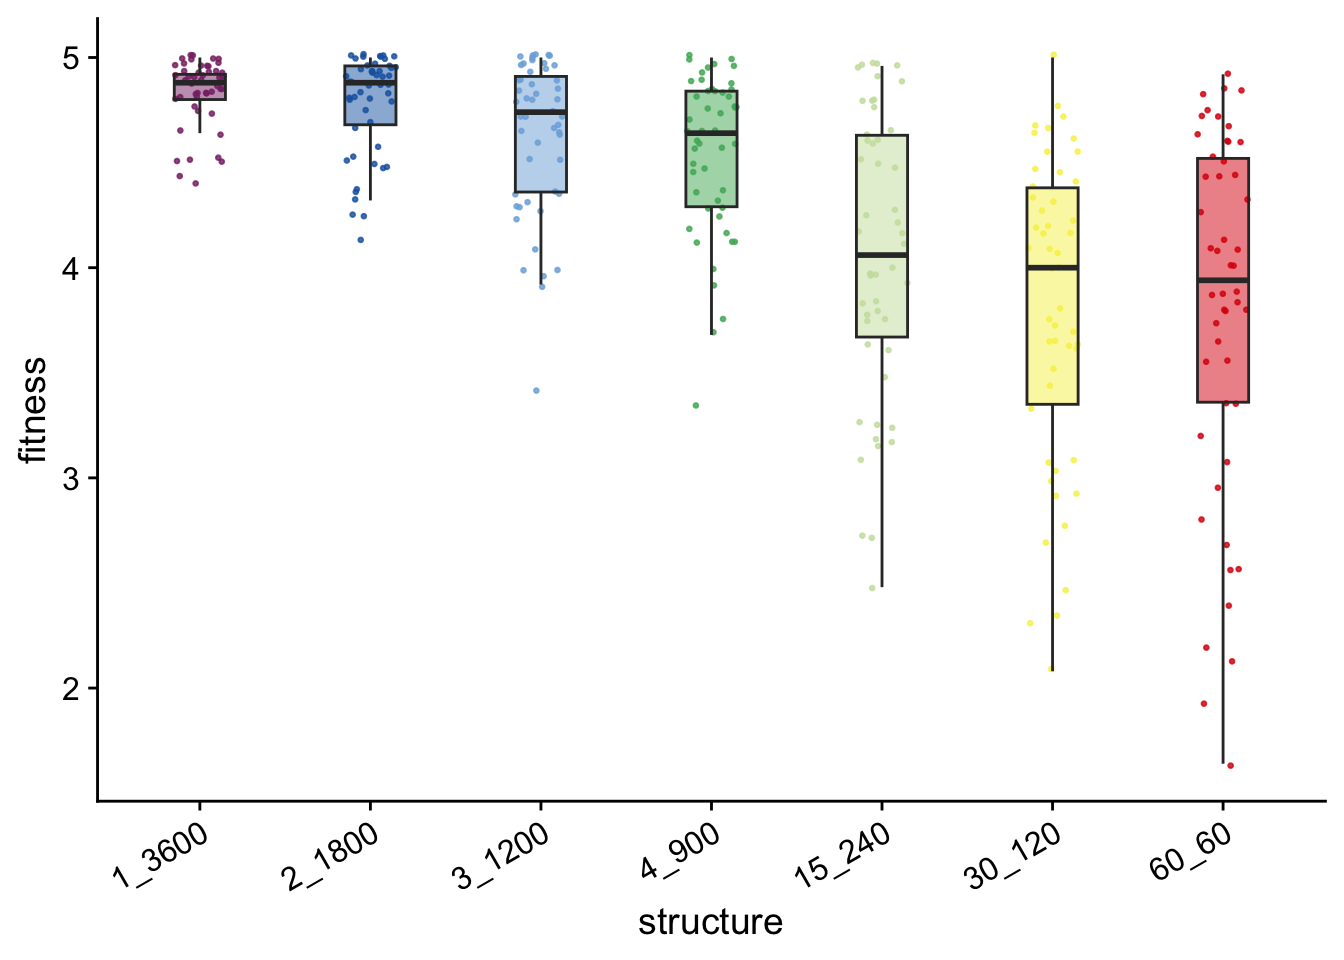
\includegraphics{supplemental-material_files/figure-latex/unnamed-chunk-35-1.pdf}

Max fitness over time

\begin{Shaded}
\begin{Highlighting}[]
\NormalTok{multipath\_fitness\_ts\_plt }\OtherTok{\textless{}{-}} \FunctionTok{ggplot}\NormalTok{(}
    \AttributeTok{data =} \FunctionTok{filter}\NormalTok{(max\_org\_data\_ts, landscape }\SpecialCharTok{==} \StringTok{"Multipath"}\NormalTok{),}
    \AttributeTok{mapping =} \FunctionTok{aes}\NormalTok{(}
      \AttributeTok{x =}\NormalTok{ generation,}
      \AttributeTok{y =}\NormalTok{ fitness,}
      \AttributeTok{color =}\NormalTok{ structure,}
      \AttributeTok{fill =}\NormalTok{ structure}
\NormalTok{    )}
\NormalTok{  ) }\SpecialCharTok{+}
  \FunctionTok{stat\_summary}\NormalTok{(}\AttributeTok{fun =} \StringTok{"mean"}\NormalTok{, }\AttributeTok{geom =} \StringTok{"line"}\NormalTok{) }\SpecialCharTok{+}
  \FunctionTok{stat\_summary}\NormalTok{(}
    \AttributeTok{fun.data =} \StringTok{"mean\_cl\_boot"}\NormalTok{,}
    \AttributeTok{fun.args =} \FunctionTok{list}\NormalTok{(}\AttributeTok{conf.int =} \FloatTok{0.95}\NormalTok{),}
    \AttributeTok{geom =} \StringTok{"ribbon"}\NormalTok{,}
    \AttributeTok{alpha =} \FloatTok{0.2}\NormalTok{,}
    \AttributeTok{linetype =} \DecValTok{0}
\NormalTok{  ) }\SpecialCharTok{+}
  \FunctionTok{theme}\NormalTok{(}\AttributeTok{legend.position =} \StringTok{"bottom"}\NormalTok{)}

\FunctionTok{ggsave}\NormalTok{(}
  \AttributeTok{plot =}\NormalTok{ multipath\_fitness\_ts\_plt,}
  \AttributeTok{filename =} \FunctionTok{paste0}\NormalTok{(}
\NormalTok{    plot\_dir,}
    \StringTok{"/multipath\_fitness\_ts.pdf"}
\NormalTok{  ),}
  \AttributeTok{width =} \DecValTok{15}\NormalTok{,}
  \AttributeTok{height =} \DecValTok{10}
\NormalTok{)}

\NormalTok{multipath\_fitness\_ts\_plt}
\end{Highlighting}
\end{Shaded}

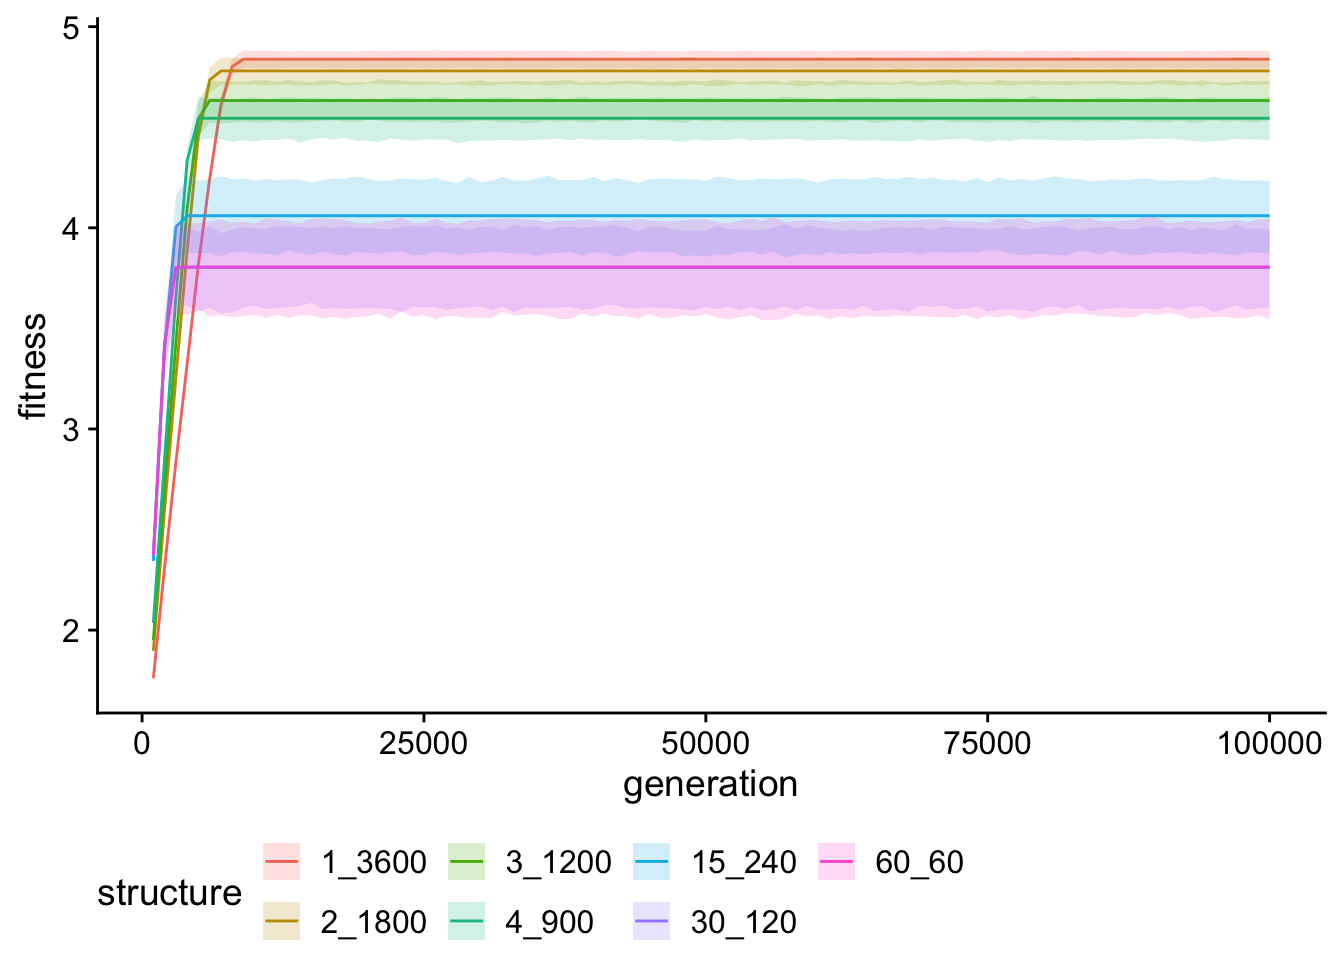
\includegraphics{supplemental-material_files/figure-latex/unnamed-chunk-36-1.pdf}

Rank ordering of fitness values

\begin{Shaded}
\begin{Highlighting}[]
\NormalTok{max\_org\_data }\SpecialCharTok{\%\textgreater{}\%}
  \FunctionTok{filter}\NormalTok{(landscape }\SpecialCharTok{==} \StringTok{"Multipath"}\NormalTok{) }\SpecialCharTok{\%\textgreater{}\%}
  \FunctionTok{group\_by}\NormalTok{(structure) }\SpecialCharTok{\%\textgreater{}\%}
  \FunctionTok{summarize}\NormalTok{(}
    \AttributeTok{reps =} \FunctionTok{n}\NormalTok{(),}
    \AttributeTok{median\_fitness =} \FunctionTok{median}\NormalTok{(fitness),}
    \AttributeTok{mean\_fitness =} \FunctionTok{mean}\NormalTok{(fitness)}
\NormalTok{  ) }\SpecialCharTok{\%\textgreater{}\%}
  \FunctionTok{arrange}\NormalTok{(}
    \FunctionTok{desc}\NormalTok{(mean\_fitness)}
\NormalTok{  )}
\end{Highlighting}
\end{Shaded}

\begin{verbatim}
## # A tibble: 7 x 4
##   structure  reps median_fitness mean_fitness
##   <fct>     <int>          <dbl>        <dbl>
## 1 1_3600       50           4.88         4.84
## 2 2_1800       50           4.88         4.78
## 3 3_1200       50           4.74         4.63
## 4 4_900        50           4.64         4.54
## 5 15_240       50           4.06         4.06
## 6 60_60        50           3.94         3.81
## 7 30_120       50           4            3.80
\end{verbatim}

\begin{Shaded}
\begin{Highlighting}[]
\FunctionTok{kruskal.test}\NormalTok{(}
  \AttributeTok{formula =}\NormalTok{ fitness }\SpecialCharTok{\textasciitilde{}}\NormalTok{ structure,}
  \AttributeTok{data =} \FunctionTok{filter}\NormalTok{(max\_org\_data, landscape }\SpecialCharTok{==} \StringTok{"Multipath"}\NormalTok{)}
\NormalTok{)}
\end{Highlighting}
\end{Shaded}

\begin{verbatim}
## 
##  Kruskal-Wallis rank sum test
## 
## data:  fitness by structure
## Kruskal-Wallis chi-squared = 144.73, df = 6, p-value < 2.2e-16
\end{verbatim}

\begin{Shaded}
\begin{Highlighting}[]
\NormalTok{wc\_results }\OtherTok{\textless{}{-}} \FunctionTok{pairwise.wilcox.test}\NormalTok{(}
  \AttributeTok{x =} \FunctionTok{filter}\NormalTok{(max\_org\_data, landscape }\SpecialCharTok{==} \StringTok{"Multipath"}\NormalTok{)}\SpecialCharTok{$}\NormalTok{fitness,}
  \AttributeTok{g =} \FunctionTok{filter}\NormalTok{(max\_org\_data, landscape }\SpecialCharTok{==} \StringTok{"Multipath"}\NormalTok{)}\SpecialCharTok{$}\NormalTok{structure,}
  \AttributeTok{p.adjust.method   =} \StringTok{"holm"}\NormalTok{,}
  \AttributeTok{exact =} \ConstantTok{FALSE}
\NormalTok{)}

\NormalTok{mp\_fitness\_wc\_table }\OtherTok{\textless{}{-}} \FunctionTok{kbl}\NormalTok{(wc\_results}\SpecialCharTok{$}\NormalTok{p.value) }\SpecialCharTok{\%\textgreater{}\%}
  \FunctionTok{kable\_styling}\NormalTok{()}

\FunctionTok{save\_kable}\NormalTok{(}
\NormalTok{  mp\_fitness\_wc\_table,}
  \FunctionTok{paste0}\NormalTok{(plot\_dir, }\StringTok{"/multipath\_fitness\_wc\_table.pdf"}\NormalTok{)}
\NormalTok{)}
\NormalTok{mp\_fitness\_wc\_table}
\end{Highlighting}
\end{Shaded}

\begin{table}
\centering
\begin{tabular}[t]{l|r|r|r|r|r|r}
\hline
  & 1\_3600 & 2\_1800 & 3\_1200 & 4\_900 & 15\_240 & 30\_120\\
\hline
2\_1800 & 1.0000000 & NA & NA & NA & NA & NA\\
\hline
3\_1200 & 0.0389539 & 0.2309342 & NA & NA & NA & NA\\
\hline
4\_900 & 0.0000552 & 0.0022081 & 0.6036094 & NA & NA & NA\\
\hline
15\_240 & 0.0000000 & 0.0000001 & 0.0000387 & 0.0022081 & NA & NA\\
\hline
30\_120 & 0.0000000 & 0.0000000 & 0.0000000 & 0.0000003 & 0.4456978 & NA\\
\hline
60\_60 & 0.0000000 & 0.0000000 & 0.0000002 & 0.0000094 & 0.6036094 & 1\\
\hline
\end{tabular}
\end{table}

\hypertarget{valleys-crossed-in-valley-crossing-landscape-1}{%
\subsection{Valleys crossed in valley-crossing landscape}\label{valleys-crossed-in-valley-crossing-landscape-1}}

\begin{Shaded}
\begin{Highlighting}[]
\NormalTok{valleycrossing\_valleys\_plt }\OtherTok{\textless{}{-}} \FunctionTok{ggplot}\NormalTok{(}
    \AttributeTok{data =} \FunctionTok{filter}\NormalTok{(max\_org\_data, landscape }\SpecialCharTok{==} \StringTok{"Valley crossing"}\NormalTok{),}
    \AttributeTok{mapping =} \FunctionTok{aes}\NormalTok{(}
      \AttributeTok{x =}\NormalTok{ structure,}
      \AttributeTok{y =}\NormalTok{ valleys\_crossed,}
      \AttributeTok{fill =}\NormalTok{ structure}
\NormalTok{    )}
\NormalTok{  ) }\SpecialCharTok{+}
  \CommentTok{\# geom\_flat\_violin(}
  \CommentTok{\#   position = position\_nudge(x = .2, y = 0),}
  \CommentTok{\#   alpha = .8}
  \CommentTok{\# ) +}
  \FunctionTok{geom\_point}\NormalTok{(}
    \AttributeTok{mapping =} \FunctionTok{aes}\NormalTok{(}\AttributeTok{color =}\NormalTok{ structure),}
    \AttributeTok{position =} \FunctionTok{position\_jitter}\NormalTok{(}\AttributeTok{width =}\NormalTok{ .}\DecValTok{15}\NormalTok{),}
    \AttributeTok{size =}\NormalTok{ .}\DecValTok{5}\NormalTok{,}
    \AttributeTok{alpha =} \FloatTok{0.8}
\NormalTok{  ) }\SpecialCharTok{+}
  \FunctionTok{geom\_boxplot}\NormalTok{(}
    \AttributeTok{width =}\NormalTok{ .}\DecValTok{3}\NormalTok{,}
    \AttributeTok{outlier.shape =} \ConstantTok{NA}\NormalTok{,}
    \AttributeTok{alpha =} \FloatTok{0.5}
\NormalTok{  ) }\SpecialCharTok{+}
  \FunctionTok{scale\_color\_discreterainbow}\NormalTok{() }\SpecialCharTok{+}
  \FunctionTok{scale\_fill\_discreterainbow}\NormalTok{() }\SpecialCharTok{+}
  \FunctionTok{theme}\NormalTok{(}
    \AttributeTok{legend.position =} \StringTok{"none"}\NormalTok{,}
    \AttributeTok{axis.text.x =} \FunctionTok{element\_text}\NormalTok{(}
      \AttributeTok{angle =} \DecValTok{30}\NormalTok{,}
      \AttributeTok{hjust =} \DecValTok{1}
\NormalTok{    )}
\NormalTok{  )}
\FunctionTok{ggsave}\NormalTok{(}
  \AttributeTok{filename =} \FunctionTok{paste0}\NormalTok{(plot\_dir, }\StringTok{"/valleycrossing\_valleys\_crossed.pdf"}\NormalTok{),}
  \AttributeTok{plot =}\NormalTok{ valleycrossing\_valleys\_plt,}
  \AttributeTok{width =} \DecValTok{6}\NormalTok{,}
  \AttributeTok{height =} \DecValTok{4}
\NormalTok{)}

\NormalTok{valleycrossing\_valleys\_plt}
\end{Highlighting}
\end{Shaded}

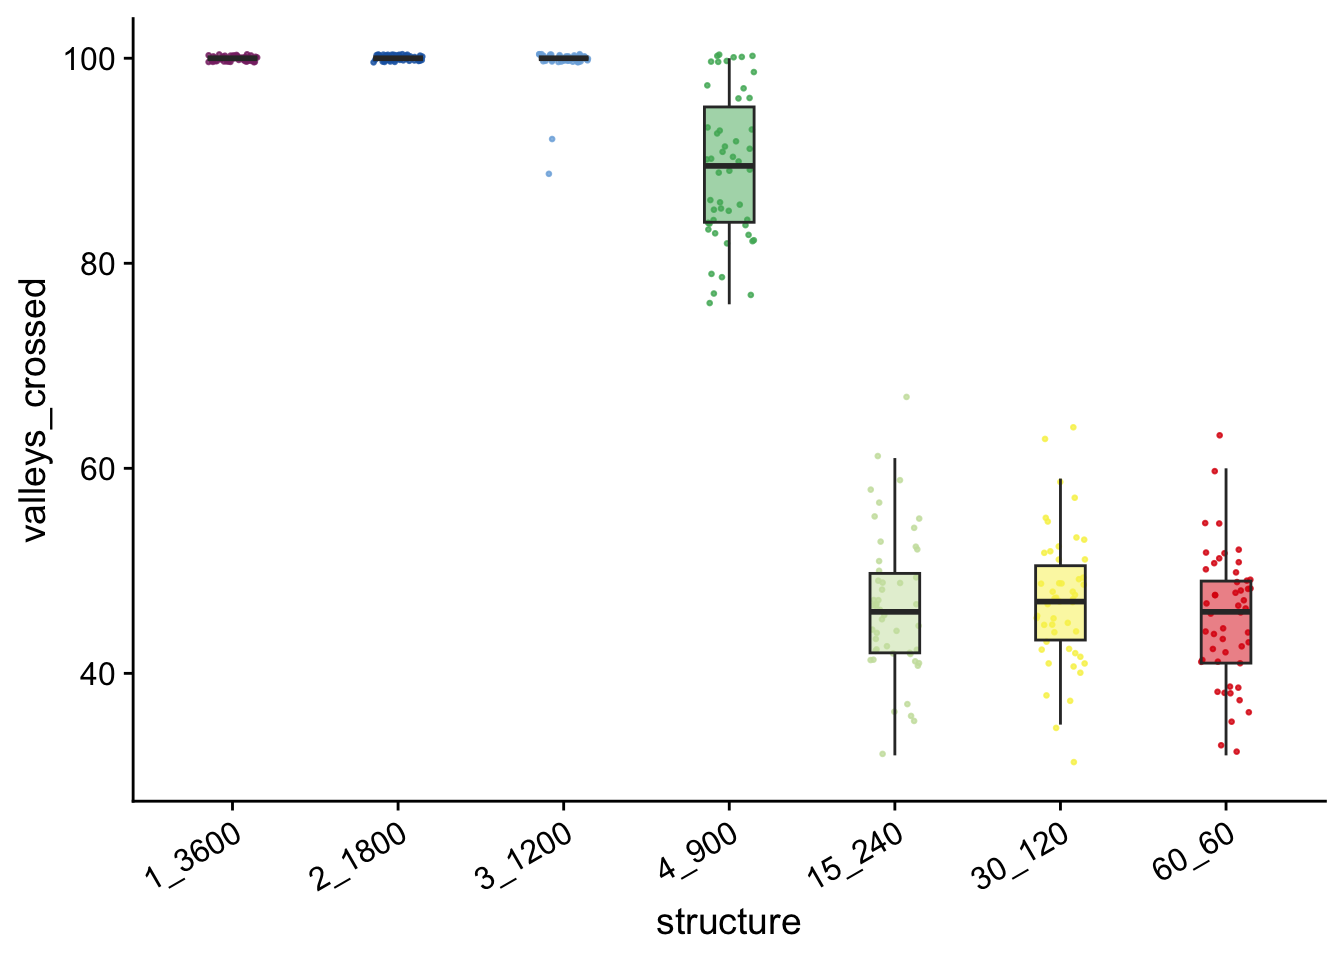
\includegraphics{supplemental-material_files/figure-latex/unnamed-chunk-39-1.pdf}

\begin{Shaded}
\begin{Highlighting}[]
\NormalTok{vc }\OtherTok{\textless{}{-}}\NormalTok{ max\_org\_data }\SpecialCharTok{\%\textgreater{}\%}
  \FunctionTok{filter}\NormalTok{(landscape }\SpecialCharTok{==} \StringTok{"Valley crossing"}\NormalTok{) }\SpecialCharTok{\%\textgreater{}\%}
  \FunctionTok{group\_by}\NormalTok{(structure) }\SpecialCharTok{\%\textgreater{}\%}
  \FunctionTok{summarize}\NormalTok{(}
    \AttributeTok{reps =} \FunctionTok{n}\NormalTok{(),}
    \AttributeTok{median\_valleys\_crossed =} \FunctionTok{median}\NormalTok{(valleys\_crossed),}
    \AttributeTok{mean\_valleys\_crossed =} \FunctionTok{mean}\NormalTok{(valleys\_crossed),}
    \AttributeTok{min\_valleys\_crossed =} \FunctionTok{min}\NormalTok{(valleys\_crossed)}
\NormalTok{  ) }\SpecialCharTok{\%\textgreater{}\%}
  \FunctionTok{arrange}\NormalTok{(}
    \FunctionTok{desc}\NormalTok{(mean\_valleys\_crossed)}
\NormalTok{  )}
\NormalTok{vc}
\end{Highlighting}
\end{Shaded}

\begin{verbatim}
## # A tibble: 7 x 5
##   structure  reps median_valleys_crossed mean_valleys_crossed
##   <fct>     <int>                  <dbl>                <dbl>
## 1 1_3600       50                  100                  100  
## 2 2_1800       50                  100                  100  
## 3 3_1200       50                  100                   99.6
## 4 4_900        50                   89.5                 89.3
## 5 30_120       50                   47                   47.2
## 6 15_240       50                   46                   46.6
## 7 60_60        50                   46                   45.5
## # i 1 more variable: min_valleys_crossed <dbl>
\end{verbatim}

\begin{Shaded}
\begin{Highlighting}[]
\NormalTok{vc}\SpecialCharTok{$}\NormalTok{min\_valleys\_crossed}
\end{Highlighting}
\end{Shaded}

\begin{verbatim}
## [1] 100 100  89  76  31  32  32
\end{verbatim}

\begin{Shaded}
\begin{Highlighting}[]
\FunctionTok{kruskal.test}\NormalTok{(}
  \AttributeTok{formula =}\NormalTok{ valleys\_crossed }\SpecialCharTok{\textasciitilde{}}\NormalTok{ structure,}
  \AttributeTok{data =} \FunctionTok{filter}\NormalTok{(max\_org\_data, landscape }\SpecialCharTok{==} \StringTok{"Valley crossing"}\NormalTok{)}
\NormalTok{)}
\end{Highlighting}
\end{Shaded}

\begin{verbatim}
## 
##  Kruskal-Wallis rank sum test
## 
## data:  valleys_crossed by structure
## Kruskal-Wallis chi-squared = 309.49, df = 6, p-value < 2.2e-16
\end{verbatim}

\begin{Shaded}
\begin{Highlighting}[]
\NormalTok{wc\_results }\OtherTok{\textless{}{-}} \FunctionTok{pairwise.wilcox.test}\NormalTok{(}
  \AttributeTok{x =} \FunctionTok{filter}\NormalTok{(max\_org\_data, landscape }\SpecialCharTok{==} \StringTok{"Valley crossing"}\NormalTok{)}\SpecialCharTok{$}\NormalTok{valleys\_crossed,}
  \AttributeTok{g =} \FunctionTok{filter}\NormalTok{(max\_org\_data, landscape }\SpecialCharTok{==} \StringTok{"Valley crossing"}\NormalTok{)}\SpecialCharTok{$}\NormalTok{structure,}
  \AttributeTok{p.adjust.method   =} \StringTok{"holm"}\NormalTok{,}
  \AttributeTok{exact =} \ConstantTok{FALSE}
\NormalTok{)}

\NormalTok{vc\_valleys\_crossed\_wc\_table }\OtherTok{\textless{}{-}} \FunctionTok{kbl}\NormalTok{(wc\_results}\SpecialCharTok{$}\NormalTok{p.value) }\SpecialCharTok{\%\textgreater{}\%}
  \FunctionTok{kable\_styling}\NormalTok{()}

\FunctionTok{save\_kable}\NormalTok{(}
\NormalTok{  vc\_valleys\_crossed\_wc\_table,}
  \FunctionTok{paste0}\NormalTok{(plot\_dir, }\StringTok{"/valley\_crossing\_valleys\_wc\_table.pdf"}\NormalTok{)}
\NormalTok{)}
\NormalTok{vc\_valleys\_crossed\_wc\_table}
\end{Highlighting}
\end{Shaded}

\begin{table}
\centering
\begin{tabular}[t]{l|r|r|r|r|r|r}
\hline
  & 1\_3600 & 2\_1800 & 3\_1200 & 4\_900 & 15\_240 & 30\_120\\
\hline
2\_1800 & NaN & NA & NA & NA & NA & NA\\
\hline
3\_1200 & 0.796952 & 0.796952 & NA & NA & NA & NA\\
\hline
4\_900 & 0.000000 & 0.000000 & 0 & NA & NA & NA\\
\hline
15\_240 & 0.000000 & 0.000000 & 0 & 0 & NA & NA\\
\hline
30\_120 & 0.000000 & 0.000000 & 0 & 0 & 0.9787605 & NA\\
\hline
60\_60 & 0.000000 & 0.000000 & 0 & 0 & 0.9787605 & 0.796952\\
\hline
\end{tabular}
\end{table}

\hypertarget{avida---varied-graph-structure-experiment-analyses}{%
\chapter{Avida - Varied graph structure experiment analyses}\label{avida---varied-graph-structure-experiment-analyses}}

\hypertarget{dependencies-and-setup-1}{%
\section{Dependencies and setup}\label{dependencies-and-setup-1}}

\begin{Shaded}
\begin{Highlighting}[]
\FunctionTok{library}\NormalTok{(tidyverse)}
\FunctionTok{library}\NormalTok{(cowplot)}
\FunctionTok{library}\NormalTok{(RColorBrewer)}
\FunctionTok{library}\NormalTok{(khroma)}
\FunctionTok{library}\NormalTok{(rstatix)}
\FunctionTok{library}\NormalTok{(knitr)}
\FunctionTok{library}\NormalTok{(kableExtra)}
\FunctionTok{source}\NormalTok{(}\StringTok{"https://gist.githubusercontent.com/benmarwick/2a1bb0133ff568cbe28d/raw/fb53bd97121f7f9ce947837ef1a4c65a73bffb3f/geom\_flat\_violin.R"}\NormalTok{)}
\end{Highlighting}
\end{Shaded}

\begin{Shaded}
\begin{Highlighting}[]
\CommentTok{\# Check if Rmd is being compiled using bookdown}
\NormalTok{bookdown }\OtherTok{\textless{}{-}} \FunctionTok{exists}\NormalTok{(}\StringTok{"bookdown\_build"}\NormalTok{)}
\end{Highlighting}
\end{Shaded}

\begin{Shaded}
\begin{Highlighting}[]
\NormalTok{experiment\_slug }\OtherTok{\textless{}{-}} \StringTok{"2025{-}04{-}17{-}vary{-}structs"}
\NormalTok{working\_directory }\OtherTok{\textless{}{-}} \FunctionTok{paste}\NormalTok{(}
  \StringTok{"experiments"}\NormalTok{,}
\NormalTok{  experiment\_slug,}
  \StringTok{"analysis"}\NormalTok{,}
  \AttributeTok{sep =} \StringTok{"/"}
\NormalTok{)}
\CommentTok{\# Adjust working directory if being knitted for bookdown build.}
\ControlFlowTok{if}\NormalTok{ (bookdown) \{}
\NormalTok{  working\_directory }\OtherTok{\textless{}{-}} \FunctionTok{paste0}\NormalTok{(}
\NormalTok{    bookdown\_wd\_prefix,}
\NormalTok{    working\_directory}
\NormalTok{  )}
\NormalTok{\}}
\end{Highlighting}
\end{Shaded}

\begin{Shaded}
\begin{Highlighting}[]
\CommentTok{\# Configure our default graphing theme}
\FunctionTok{theme\_set}\NormalTok{(}\FunctionTok{theme\_cowplot}\NormalTok{())}
\CommentTok{\# Create a directory to store plots}
\NormalTok{plot\_dir }\OtherTok{\textless{}{-}} \FunctionTok{paste}\NormalTok{(}
\NormalTok{  working\_directory,}
  \StringTok{"plots"}\NormalTok{,}
  \AttributeTok{sep =} \StringTok{"/"}
\NormalTok{)}

\FunctionTok{dir.create}\NormalTok{(}
\NormalTok{  plot\_dir,}
  \AttributeTok{showWarnings =} \ConstantTok{FALSE}
\NormalTok{)}
\end{Highlighting}
\end{Shaded}

\begin{Shaded}
\begin{Highlighting}[]
\NormalTok{focal\_graphs }\OtherTok{\textless{}{-}} \FunctionTok{c}\NormalTok{(}
  \StringTok{"star"}\NormalTok{,}
  \StringTok{"random{-}waxman"}\NormalTok{,}
  \StringTok{"comet{-}kite"}\NormalTok{,}
  \StringTok{"linear{-}chain"}\NormalTok{,}
  \StringTok{"cycle"}\NormalTok{,}
  \StringTok{"clique{-}ring"}\NormalTok{,}
  \StringTok{"toroidal{-}lattice"}\NormalTok{,}
  \StringTok{"well{-}mixed"}\NormalTok{,}
  \StringTok{"wheel"}\NormalTok{,}
  \StringTok{"windmill"}
\NormalTok{)}

\CommentTok{\# Load summary data from final update}
\NormalTok{data\_path }\OtherTok{\textless{}{-}} \FunctionTok{paste}\NormalTok{(}
\NormalTok{  working\_directory,}
  \StringTok{"data"}\NormalTok{,}
  \StringTok{"summary.csv"}\NormalTok{,}
  \AttributeTok{sep =} \StringTok{"/"}
\NormalTok{)}
\NormalTok{data }\OtherTok{\textless{}{-}} \FunctionTok{read\_csv}\NormalTok{(data\_path)}

\NormalTok{data }\OtherTok{\textless{}{-}}\NormalTok{ data }\SpecialCharTok{\%\textgreater{}\%}
  \FunctionTok{mutate}\NormalTok{(}
    \AttributeTok{graph\_type =} \FunctionTok{factor}\NormalTok{(}
\NormalTok{      graph\_type,}
      \AttributeTok{levels =} \FunctionTok{c}\NormalTok{(}
        \StringTok{"star"}\NormalTok{,}
        \StringTok{"random{-}waxman"}\NormalTok{,}
        \StringTok{"comet{-}kite"}\NormalTok{,}
        \StringTok{"linear{-}chain"}\NormalTok{,}
        \StringTok{"cycle"}\NormalTok{,}
        \StringTok{"clique{-}ring"}\NormalTok{,}
        \StringTok{"toroidal{-}lattice"}\NormalTok{,}
        \StringTok{"well{-}mixed"}\NormalTok{,}
        \StringTok{"wheel"}\NormalTok{,}
        \StringTok{"windmill"}
\NormalTok{      )}
\NormalTok{    ),}
    \AttributeTok{ENVIRONMENT\_FILE =} \FunctionTok{as.factor}\NormalTok{(ENVIRONMENT\_FILE)}
\NormalTok{  )}
\NormalTok{data }\OtherTok{\textless{}{-}}\NormalTok{ data }\SpecialCharTok{\%\textgreater{}\%} \FunctionTok{filter}\NormalTok{(}
\NormalTok{  graph\_type }\SpecialCharTok{\%in\%}\NormalTok{ focal\_graphs}
\NormalTok{)}
\NormalTok{data }\OtherTok{\textless{}{-}}\NormalTok{ data }\SpecialCharTok{\%\textgreater{}\%} \FunctionTok{filter}\NormalTok{(reached\_target\_update)}
\end{Highlighting}
\end{Shaded}

\begin{Shaded}
\begin{Highlighting}[]
\NormalTok{time\_series\_path }\OtherTok{\textless{}{-}} \FunctionTok{paste}\NormalTok{(}
\NormalTok{  working\_directory,}
  \StringTok{"data"}\NormalTok{,}
  \StringTok{"time\_series.csv"}\NormalTok{,}
  \AttributeTok{sep =} \StringTok{"/"}
\NormalTok{)}
\NormalTok{time\_series\_data }\OtherTok{\textless{}{-}} \FunctionTok{read\_csv}\NormalTok{(time\_series\_path)}

\NormalTok{time\_series\_data }\OtherTok{\textless{}{-}}\NormalTok{ time\_series\_data }\SpecialCharTok{\%\textgreater{}\%}
  \FunctionTok{mutate}\NormalTok{(}
    \AttributeTok{graph\_type =} \FunctionTok{factor}\NormalTok{(}
\NormalTok{      graph\_type,}
      \AttributeTok{levels =} \FunctionTok{c}\NormalTok{(}
        \StringTok{"star"}\NormalTok{,}
        \StringTok{"random{-}waxman"}\NormalTok{,}
        \StringTok{"comet{-}kite"}\NormalTok{,}
        \StringTok{"linear{-}chain"}\NormalTok{,}
        \StringTok{"cycle"}\NormalTok{,}
        \StringTok{"clique{-}ring"}\NormalTok{,}
        \StringTok{"toroidal{-}lattice"}\NormalTok{,}
        \StringTok{"well{-}mixed"}\NormalTok{,}
        \StringTok{"wheel"}\NormalTok{,}
        \StringTok{"windmill"}
\NormalTok{      )}
\NormalTok{    ),}
    \AttributeTok{ENVIRONMENT\_FILE =} \FunctionTok{as.factor}\NormalTok{(ENVIRONMENT\_FILE),}
    \AttributeTok{seed =} \FunctionTok{as.factor}\NormalTok{(seed)}
\NormalTok{  )}
\NormalTok{time\_series\_data }\OtherTok{\textless{}{-}}\NormalTok{ time\_series\_data }\SpecialCharTok{\%\textgreater{}\%} \FunctionTok{filter}\NormalTok{(seed }\SpecialCharTok{\%in\%}\NormalTok{ data}\SpecialCharTok{$}\NormalTok{seed)}
\NormalTok{time\_series\_data }\OtherTok{\textless{}{-}}\NormalTok{ time\_series\_data }\SpecialCharTok{\%\textgreater{}\%} \FunctionTok{filter}\NormalTok{(}
\NormalTok{  graph\_type }\SpecialCharTok{\%in\%}\NormalTok{ focal\_graphs}
\NormalTok{)}
\end{Highlighting}
\end{Shaded}

\begin{Shaded}
\begin{Highlighting}[]
\CommentTok{\# Check that all runs completed}
\NormalTok{data }\SpecialCharTok{\%\textgreater{}\%}
  \FunctionTok{filter}\NormalTok{(update }\SpecialCharTok{==} \DecValTok{400000}\NormalTok{) }\SpecialCharTok{\%\textgreater{}\%}
  \FunctionTok{group\_by}\NormalTok{(graph\_type) }\SpecialCharTok{\%\textgreater{}\%}
  \FunctionTok{summarize}\NormalTok{(}
    \AttributeTok{n =} \FunctionTok{n}\NormalTok{()}
\NormalTok{  )}
\end{Highlighting}
\end{Shaded}

\begin{verbatim}
## # A tibble: 10 x 2
##    graph_type           n
##    <fct>            <int>
##  1 star                50
##  2 random-waxman       50
##  3 comet-kite          50
##  4 linear-chain        50
##  5 cycle               50
##  6 clique-ring         50
##  7 toroidal-lattice    50
##  8 well-mixed          50
##  9 wheel               50
## 10 windmill            50
\end{verbatim}

\hypertarget{number-of-tasks-completed}{%
\section{Number of tasks completed}\label{number-of-tasks-completed}}

\begin{Shaded}
\begin{Highlighting}[]
\NormalTok{pop\_tasks\_total\_plt }\OtherTok{\textless{}{-}} \FunctionTok{ggplot}\NormalTok{(}
  \AttributeTok{data =}\NormalTok{ data,}
  \AttributeTok{mapping =} \FunctionTok{aes}\NormalTok{(}
    \AttributeTok{x =}\NormalTok{ graph\_type,}
    \AttributeTok{y =}\NormalTok{ pop\_task\_total,}
    \AttributeTok{fill =}\NormalTok{ graph\_type}
\NormalTok{  )}
\NormalTok{) }\SpecialCharTok{+}
  \FunctionTok{geom\_flat\_violin}\NormalTok{(}
    \AttributeTok{position =} \FunctionTok{position\_nudge}\NormalTok{(}\AttributeTok{x =}\NormalTok{ .}\DecValTok{2}\NormalTok{, }\AttributeTok{y =} \DecValTok{0}\NormalTok{),}
    \AttributeTok{alpha =}\NormalTok{ .}\DecValTok{8}
\NormalTok{  ) }\SpecialCharTok{+}
  \FunctionTok{geom\_point}\NormalTok{(}
    \AttributeTok{mapping=}\FunctionTok{aes}\NormalTok{(}\AttributeTok{color =}\NormalTok{ graph\_type),}
    \AttributeTok{position =} \FunctionTok{position\_jitter}\NormalTok{(}\AttributeTok{width =}\NormalTok{ .}\DecValTok{15}\NormalTok{),}
    \AttributeTok{size =}\NormalTok{ .}\DecValTok{5}\NormalTok{,}
    \AttributeTok{alpha =} \FloatTok{0.8}
\NormalTok{  ) }\SpecialCharTok{+}
  \FunctionTok{geom\_boxplot}\NormalTok{(}
    \AttributeTok{width =}\NormalTok{ .}\DecValTok{1}\NormalTok{,}
    \AttributeTok{outlier.shape =} \ConstantTok{NA}\NormalTok{,}
    \AttributeTok{alpha =} \FloatTok{0.5}
\NormalTok{  ) }\SpecialCharTok{+}
  \FunctionTok{theme}\NormalTok{(}
    \AttributeTok{legend.position =} \StringTok{"none"}\NormalTok{,}
    \AttributeTok{axis.text.x =} \FunctionTok{element\_text}\NormalTok{(}
      \AttributeTok{angle =} \DecValTok{30}\NormalTok{,}
      \AttributeTok{hjust =} \DecValTok{1}
\NormalTok{    )}
\NormalTok{  )}

\FunctionTok{ggsave}\NormalTok{(}
  \AttributeTok{filename =} \FunctionTok{paste0}\NormalTok{(plot\_dir, }\StringTok{"/pop\_tasks\_total.pdf"}\NormalTok{),}
  \AttributeTok{plot =}\NormalTok{ pop\_tasks\_total\_plt,}
  \AttributeTok{width =} \DecValTok{15}\NormalTok{,}
  \AttributeTok{height =} \DecValTok{10}
\NormalTok{)}

\NormalTok{pop\_tasks\_total\_plt}
\end{Highlighting}
\end{Shaded}

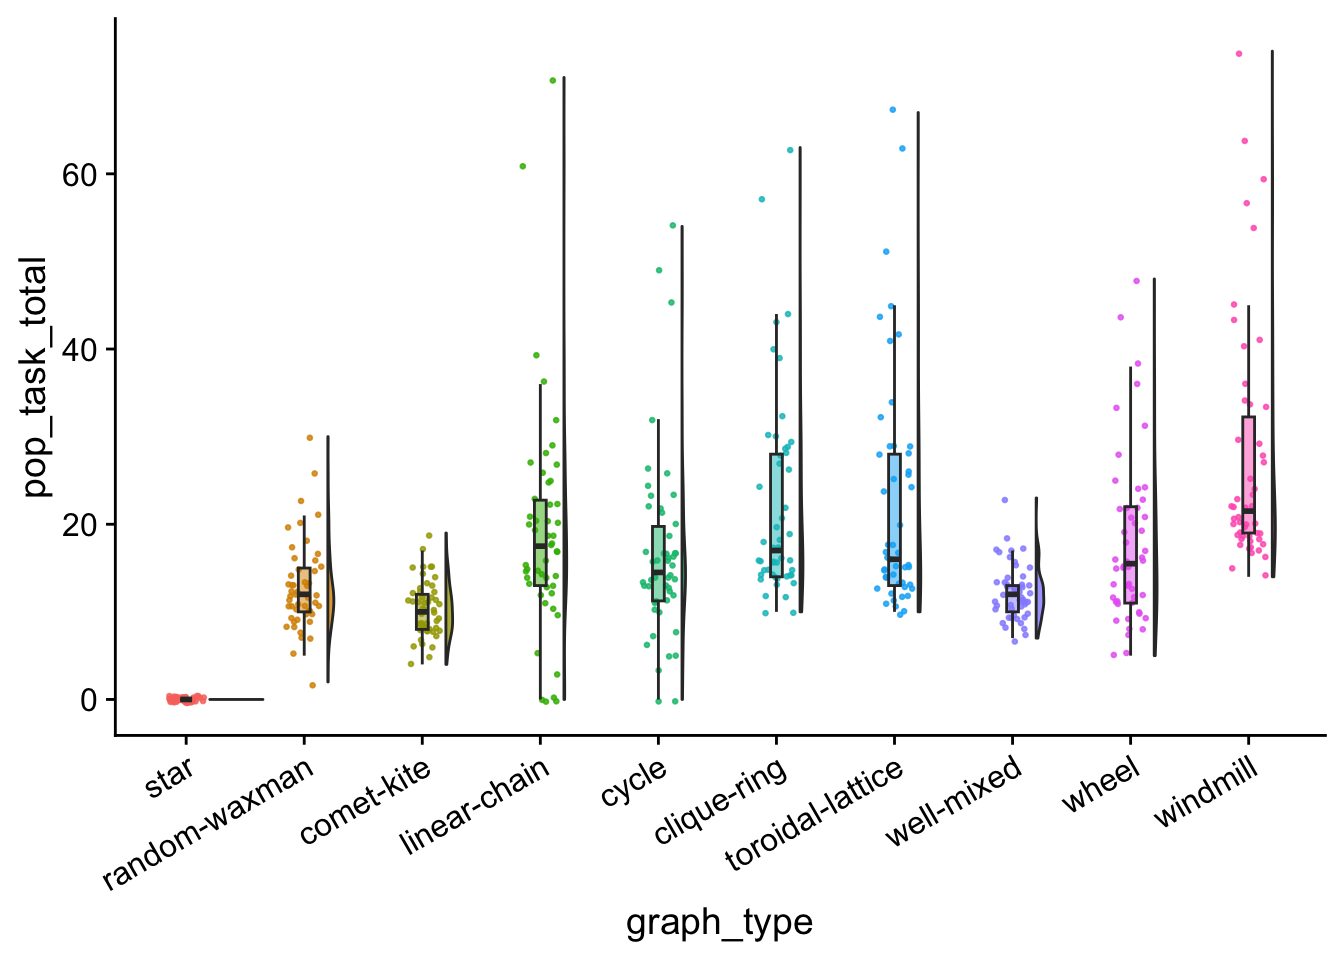
\includegraphics{supplemental-material_files/figure-latex/unnamed-chunk-49-1.pdf}

\begin{Shaded}
\begin{Highlighting}[]
\NormalTok{data }\SpecialCharTok{\%\textgreater{}\%}
  \FunctionTok{group\_by}\NormalTok{(graph\_type) }\SpecialCharTok{\%\textgreater{}\%}
  \FunctionTok{summarize}\NormalTok{(}
    \AttributeTok{reps =} \FunctionTok{n}\NormalTok{(),}
    \AttributeTok{median\_pop\_tasks =} \FunctionTok{median}\NormalTok{(pop\_task\_total),}
    \AttributeTok{mean\_pop\_tasks =} \FunctionTok{mean}\NormalTok{(pop\_task\_total)}
\NormalTok{  ) }\SpecialCharTok{\%\textgreater{}\%}
  \FunctionTok{arrange}\NormalTok{(}
    \FunctionTok{desc}\NormalTok{(mean\_pop\_tasks)}
\NormalTok{  )}
\end{Highlighting}
\end{Shaded}

\begin{verbatim}
## # A tibble: 10 x 4
##    graph_type        reps median_pop_tasks mean_pop_tasks
##    <fct>            <int>            <dbl>          <dbl>
##  1 windmill            50             21.5           27.4
##  2 toroidal-lattice    50             16             22.4
##  3 clique-ring         50             17             22.1
##  4 linear-chain        50             17.5           19.1
##  5 wheel               50             15.5           17.8
##  6 cycle               50             14.5           16.6
##  7 random-waxman       50             12             12.8
##  8 well-mixed          50             12             12.2
##  9 comet-kite          50             10             10.3
## 10 star                50              0              0
\end{verbatim}

\begin{Shaded}
\begin{Highlighting}[]
\FunctionTok{kruskal.test}\NormalTok{(}
  \AttributeTok{formula =}\NormalTok{ pop\_task\_total }\SpecialCharTok{\textasciitilde{}}\NormalTok{ graph\_type,}
  \AttributeTok{data =}\NormalTok{ data}
\NormalTok{)}
\end{Highlighting}
\end{Shaded}

\begin{verbatim}
## 
##  Kruskal-Wallis rank sum test
## 
## data:  pop_task_total by graph_type
## Kruskal-Wallis chi-squared = 252.46, df = 9, p-value < 2.2e-16
\end{verbatim}

\begin{Shaded}
\begin{Highlighting}[]
\NormalTok{wc\_results }\OtherTok{\textless{}{-}} \FunctionTok{pairwise.wilcox.test}\NormalTok{(}
  \AttributeTok{x =}\NormalTok{ data}\SpecialCharTok{$}\NormalTok{pop\_task\_total,}
  \AttributeTok{g =}\NormalTok{ data}\SpecialCharTok{$}\NormalTok{graph\_type,}
  \AttributeTok{p.adjust.method   =} \StringTok{"holm"}\NormalTok{,}
  \AttributeTok{exact =} \ConstantTok{FALSE}
\NormalTok{)}

\NormalTok{pop\_task\_wc\_table }\OtherTok{\textless{}{-}} \FunctionTok{kbl}\NormalTok{(wc\_results}\SpecialCharTok{$}\NormalTok{p.value) }\SpecialCharTok{\%\textgreater{}\%} \FunctionTok{kable\_styling}\NormalTok{()}
\FunctionTok{save\_kable}\NormalTok{(pop\_task\_wc\_table, }\FunctionTok{paste0}\NormalTok{(plot\_dir, }\StringTok{"/pop\_task\_wc\_table.pdf"}\NormalTok{))}
\NormalTok{pop\_task\_wc\_table}
\end{Highlighting}
\end{Shaded}

\begin{table}
\centering
\begin{tabular}[t]{l|r|r|r|r|r|r|r|r|r}
\hline
  & star & random-waxman & comet-kite & linear-chain & cycle & clique-ring & toroidal-lattice & well-mixed & wheel\\
\hline
random-waxman & 0 & NA & NA & NA & NA & NA & NA & NA & NA\\
\hline
comet-kite & 0 & 0.0755715 & NA & NA & NA & NA & NA & NA & NA\\
\hline
linear-chain & 0 & 0.0040473 & 0.0000027 & NA & NA & NA & NA & NA & NA\\
\hline
cycle & 0 & 0.1530200 & 0.0002750 & 1.0000000 & NA & NA & NA & NA & NA\\
\hline
clique-ring & 0 & 0.0000008 & 0.0000000 & 1.0000000 & 0.0702670 & NA & NA & NA & NA\\
\hline
toroidal-lattice & 0 & 0.0000297 & 0.0000000 & 1.0000000 & 0.3032752 & 1.0000000 & NA & NA & NA\\
\hline
well-mixed & 0 & 1.0000000 & 0.0542973 & 0.0002739 & 0.0505844 & 0.0000000 & 0.0000018 & NA & NA\\
\hline
wheel & 0 & 0.0681554 & 0.0000297 & 1.0000000 & 1.0000000 & 0.2644489 & 0.6033308 & 0.0280284 & NA\\
\hline
windmill & 0 & 0.0000000 & 0.0000000 & 0.0058779 & 0.0000035 & 0.0302955 & 0.0302955 & 0.0000000 & 0.000275\\
\hline
\end{tabular}
\end{table}

\hypertarget{dominant-tasks}{%
\section{Dominant tasks}\label{dominant-tasks}}

\begin{Shaded}
\begin{Highlighting}[]
\NormalTok{dom\_tasks\_total\_plt }\OtherTok{\textless{}{-}} \FunctionTok{ggplot}\NormalTok{(}
  \AttributeTok{data =}\NormalTok{ data,}
  \AttributeTok{mapping =} \FunctionTok{aes}\NormalTok{(}
    \AttributeTok{x =}\NormalTok{ graph\_type,}
    \AttributeTok{y =}\NormalTok{ dom\_task\_total,}
    \AttributeTok{fill =}\NormalTok{ graph\_type}
\NormalTok{  )}
\NormalTok{) }\SpecialCharTok{+}
  \FunctionTok{geom\_flat\_violin}\NormalTok{(}
    \AttributeTok{position =} \FunctionTok{position\_nudge}\NormalTok{(}\AttributeTok{x =}\NormalTok{ .}\DecValTok{2}\NormalTok{, }\AttributeTok{y =} \DecValTok{0}\NormalTok{),}
    \AttributeTok{alpha =}\NormalTok{ .}\DecValTok{8}
\NormalTok{  ) }\SpecialCharTok{+}
  \FunctionTok{geom\_point}\NormalTok{(}
    \AttributeTok{mapping=}\FunctionTok{aes}\NormalTok{(}\AttributeTok{color =}\NormalTok{ graph\_type),}
    \AttributeTok{position =} \FunctionTok{position\_jitter}\NormalTok{(}\AttributeTok{width =}\NormalTok{ .}\DecValTok{15}\NormalTok{),}
    \AttributeTok{size =}\NormalTok{ .}\DecValTok{5}\NormalTok{,}
    \AttributeTok{alpha =} \FloatTok{0.8}
\NormalTok{  ) }\SpecialCharTok{+}
  \FunctionTok{geom\_boxplot}\NormalTok{(}
    \AttributeTok{width =}\NormalTok{ .}\DecValTok{1}\NormalTok{,}
    \AttributeTok{outlier.shape =} \ConstantTok{NA}\NormalTok{,}
    \AttributeTok{alpha =} \FloatTok{0.5}
\NormalTok{  ) }\SpecialCharTok{+}
  \FunctionTok{theme}\NormalTok{(}
    \AttributeTok{legend.position =} \StringTok{"none"}\NormalTok{,}
    \AttributeTok{axis.text.x =} \FunctionTok{element\_text}\NormalTok{(}
      \AttributeTok{angle =} \DecValTok{30}\NormalTok{,}
      \AttributeTok{hjust =} \DecValTok{1}
\NormalTok{    )}
\NormalTok{  )}

\FunctionTok{ggsave}\NormalTok{(}
  \AttributeTok{filename =} \FunctionTok{paste0}\NormalTok{(plot\_dir, }\StringTok{"/dom\_tasks\_total.pdf"}\NormalTok{),}
  \AttributeTok{plot =}\NormalTok{ dom\_tasks\_total\_plt,}
  \AttributeTok{width =} \DecValTok{15}\NormalTok{,}
  \AttributeTok{height =} \DecValTok{10}
\NormalTok{)}

\NormalTok{dom\_tasks\_total\_plt}
\end{Highlighting}
\end{Shaded}

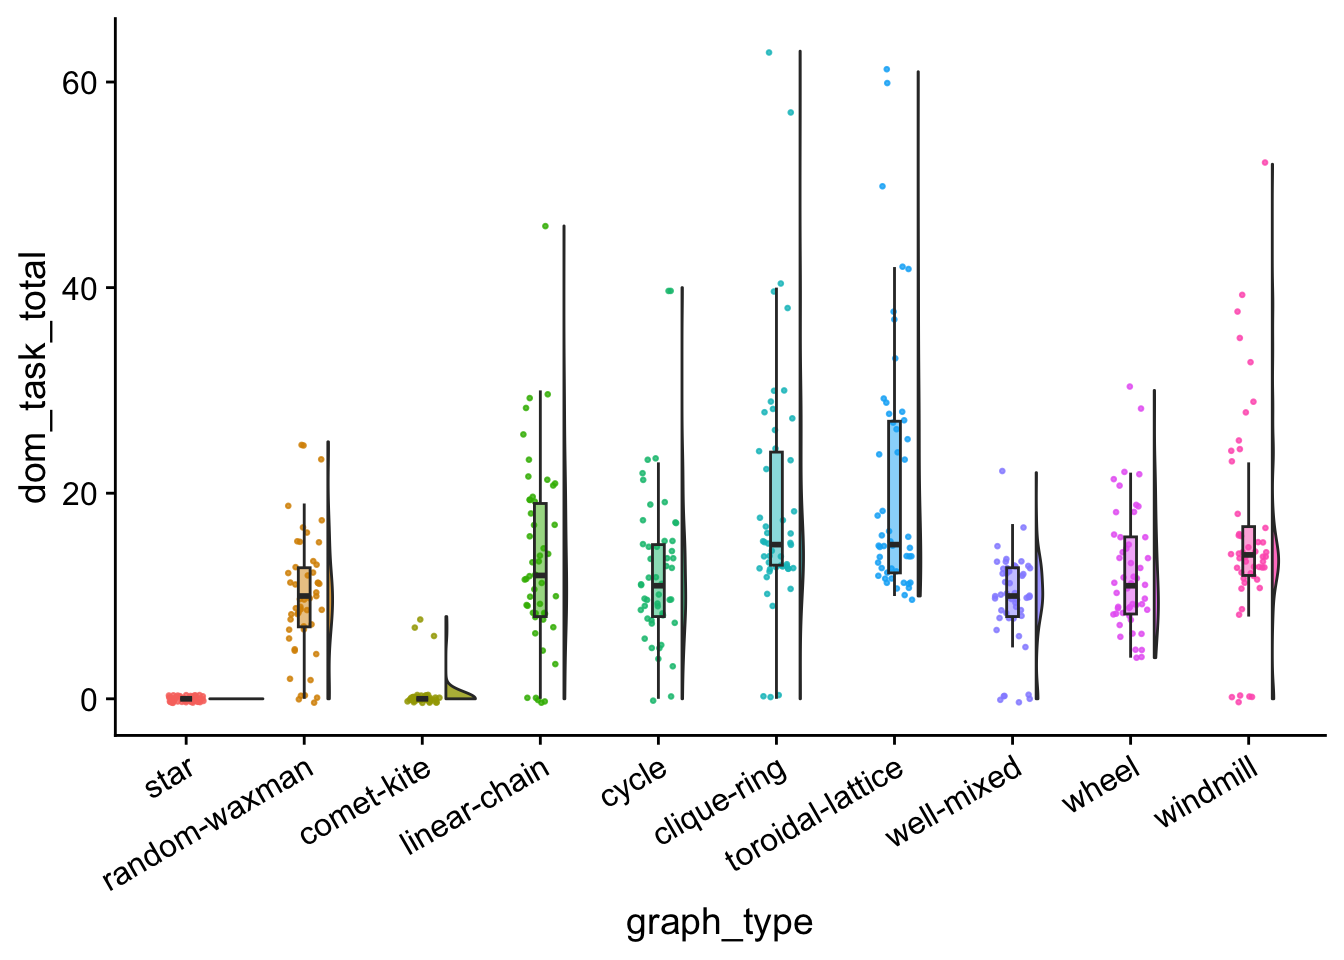
\includegraphics{supplemental-material_files/figure-latex/unnamed-chunk-52-1.pdf}

\begin{Shaded}
\begin{Highlighting}[]
\NormalTok{data }\SpecialCharTok{\%\textgreater{}\%}
  \FunctionTok{group\_by}\NormalTok{(graph\_type) }\SpecialCharTok{\%\textgreater{}\%}
  \FunctionTok{summarize}\NormalTok{(}
    \AttributeTok{reps =} \FunctionTok{n}\NormalTok{(),}
    \AttributeTok{median\_dom\_task\_total =} \FunctionTok{median}\NormalTok{(dom\_task\_total),}
    \AttributeTok{mean\_dom\_task\_total =} \FunctionTok{mean}\NormalTok{(dom\_task\_total)}
\NormalTok{  ) }\SpecialCharTok{\%\textgreater{}\%}
  \FunctionTok{arrange}\NormalTok{(}
    \FunctionTok{desc}\NormalTok{(mean\_dom\_task\_total)}
\NormalTok{  )}
\end{Highlighting}
\end{Shaded}

\begin{verbatim}
## # A tibble: 10 x 4
##    graph_type        reps median_dom_task_total mean_dom_task_total
##    <fct>            <int>                 <dbl>               <dbl>
##  1 toroidal-lattice    50                    15               21.4 
##  2 clique-ring         50                    15               19.2 
##  3 windmill            50                    14               16.1 
##  4 linear-chain        50                    12               13.6 
##  5 cycle               50                    11               12.6 
##  6 wheel               50                    11               12.4 
##  7 random-waxman       50                    10                9.92
##  8 well-mixed          50                    10                9.62
##  9 comet-kite          50                     0                0.42
## 10 star                50                     0                0
\end{verbatim}

\begin{Shaded}
\begin{Highlighting}[]
\FunctionTok{kruskal.test}\NormalTok{(}
  \AttributeTok{formula =}\NormalTok{ dom\_task\_total }\SpecialCharTok{\textasciitilde{}}\NormalTok{ graph\_type,}
  \AttributeTok{data =}\NormalTok{ data}
\NormalTok{)}
\end{Highlighting}
\end{Shaded}

\begin{verbatim}
## 
##  Kruskal-Wallis rank sum test
## 
## data:  dom_task_total by graph_type
## Kruskal-Wallis chi-squared = 262.43, df = 9, p-value < 2.2e-16
\end{verbatim}

\begin{Shaded}
\begin{Highlighting}[]
\NormalTok{wc\_results }\OtherTok{\textless{}{-}} \FunctionTok{pairwise.wilcox.test}\NormalTok{(}
  \AttributeTok{x =}\NormalTok{ data}\SpecialCharTok{$}\NormalTok{dom\_task\_total,}
  \AttributeTok{g =}\NormalTok{ data}\SpecialCharTok{$}\NormalTok{graph\_type,}
  \AttributeTok{p.adjust.method   =} \StringTok{"holm"}\NormalTok{,}
  \AttributeTok{exact =} \ConstantTok{FALSE}
\NormalTok{)}

\NormalTok{dom\_task\_total\_wc\_table }\OtherTok{\textless{}{-}} \FunctionTok{kbl}\NormalTok{(wc\_results}\SpecialCharTok{$}\NormalTok{p.value) }\SpecialCharTok{\%\textgreater{}\%} \FunctionTok{kable\_styling}\NormalTok{()}
\FunctionTok{save\_kable}\NormalTok{(dom\_task\_total\_wc\_table, }\FunctionTok{paste0}\NormalTok{(plot\_dir, }\StringTok{"/dom\_task\_total\_wc\_table.pdf"}\NormalTok{))}
\NormalTok{dom\_task\_total\_wc\_table}
\end{Highlighting}
\end{Shaded}

\begin{table}
\centering
\begin{tabular}[t]{l|r|r|r|r|r|r|r|r|r}
\hline
  & star & random-waxman & comet-kite & linear-chain & cycle & clique-ring & toroidal-lattice & well-mixed & wheel\\
\hline
random-waxman & 0.0000000 & NA & NA & NA & NA & NA & NA & NA & NA\\
\hline
comet-kite & 0.9646146 & 0.0000000 & NA & NA & NA & NA & NA & NA & NA\\
\hline
linear-chain & 0.0000000 & 0.4710663 & 0 & NA & NA & NA & NA & NA & NA\\
\hline
cycle & 0.0000000 & 0.9646146 & 0 & 1.0000000 & NA & NA & NA & NA & NA\\
\hline
clique-ring & 0.0000000 & 0.0000042 & 0 & 0.0907079 & 0.0083936 & NA & NA & NA & NA\\
\hline
toroidal-lattice & 0.0000000 & 0.0000001 & 0 & 0.0112805 & 0.0003268 & 1.0000000 & NA & NA & NA\\
\hline
well-mixed & 0.0000000 & 1.0000000 & 0 & 0.5076566 & 0.9646146 & 0.0000000 & 0.0000000 & NA & NA\\
\hline
wheel & 0.0000000 & 0.9646146 & 0 & 1.0000000 & 1.0000000 & 0.0033520 & 0.0001346 & 0.9865397 & NA\\
\hline
windmill & 0.0000000 & 0.0009903 & 0 & 0.9865397 & 0.4321933 & 0.9865397 & 0.7677082 & 0.0000305 & 0.2316497\\
\hline
\end{tabular}
\end{table}

Tasks done by organisms not in dominant taxon:

\begin{Shaded}
\begin{Highlighting}[]
\NormalTok{data }\OtherTok{\textless{}{-}}\NormalTok{ data }\SpecialCharTok{\%\textgreater{}\%}
  \FunctionTok{mutate}\NormalTok{(}
    \AttributeTok{nondom\_pop\_task\_prop =} \FunctionTok{case\_when}\NormalTok{(}
\NormalTok{      pop\_task\_total }\SpecialCharTok{==} \DecValTok{0} \SpecialCharTok{\textasciitilde{}} \DecValTok{0}\NormalTok{,}
      \AttributeTok{.default =}\NormalTok{ (pop\_task\_total }\SpecialCharTok{{-}}\NormalTok{ dom\_task\_total) }\SpecialCharTok{/}\NormalTok{ (pop\_task\_total)}
\NormalTok{    )}
\NormalTok{  )}

\NormalTok{nondom\_tasks\_total\_plt }\OtherTok{\textless{}{-}} \FunctionTok{ggplot}\NormalTok{(}
    \AttributeTok{data =}\NormalTok{ data,}
    \AttributeTok{mapping =} \FunctionTok{aes}\NormalTok{(}
      \AttributeTok{x =}\NormalTok{ graph\_type,}
      \AttributeTok{y =}\NormalTok{ nondom\_pop\_task\_prop,}
      \AttributeTok{fill =}\NormalTok{ graph\_type}
\NormalTok{    )}
\NormalTok{  ) }\SpecialCharTok{+}
  \FunctionTok{geom\_flat\_violin}\NormalTok{(}
    \AttributeTok{position =} \FunctionTok{position\_nudge}\NormalTok{(}\AttributeTok{x =}\NormalTok{ .}\DecValTok{2}\NormalTok{, }\AttributeTok{y =} \DecValTok{0}\NormalTok{),}
    \AttributeTok{alpha =}\NormalTok{ .}\DecValTok{8}
\NormalTok{  ) }\SpecialCharTok{+}
  \FunctionTok{geom\_point}\NormalTok{(}
    \AttributeTok{mapping=}\FunctionTok{aes}\NormalTok{(}\AttributeTok{color =}\NormalTok{ graph\_type),}
    \AttributeTok{position =} \FunctionTok{position\_jitter}\NormalTok{(}\AttributeTok{width =}\NormalTok{ .}\DecValTok{15}\NormalTok{),}
    \AttributeTok{size =}\NormalTok{ .}\DecValTok{5}\NormalTok{,}
    \AttributeTok{alpha =} \FloatTok{0.8}
\NormalTok{  ) }\SpecialCharTok{+}
  \FunctionTok{geom\_boxplot}\NormalTok{(}
    \AttributeTok{width =}\NormalTok{ .}\DecValTok{1}\NormalTok{,}
    \AttributeTok{outlier.shape =} \ConstantTok{NA}\NormalTok{,}
    \AttributeTok{alpha =} \FloatTok{0.5}
\NormalTok{  ) }\SpecialCharTok{+}
  \FunctionTok{theme}\NormalTok{(}
    \AttributeTok{legend.position =} \StringTok{"none"}\NormalTok{,}
    \AttributeTok{axis.text.x =} \FunctionTok{element\_text}\NormalTok{(}
      \AttributeTok{angle =} \DecValTok{30}\NormalTok{,}
      \AttributeTok{hjust =} \DecValTok{1}
\NormalTok{    )}
\NormalTok{  )}

\FunctionTok{ggsave}\NormalTok{(}
  \AttributeTok{filename =} \FunctionTok{paste0}\NormalTok{(plot\_dir, }\StringTok{"/non\_dom\_tasks\_total.pdf"}\NormalTok{),}
  \AttributeTok{plot =}\NormalTok{ nondom\_tasks\_total\_plt,}
  \AttributeTok{width =} \DecValTok{15}\NormalTok{,}
  \AttributeTok{height =} \DecValTok{10}
\NormalTok{)}

\NormalTok{nondom\_tasks\_total\_plt}
\end{Highlighting}
\end{Shaded}

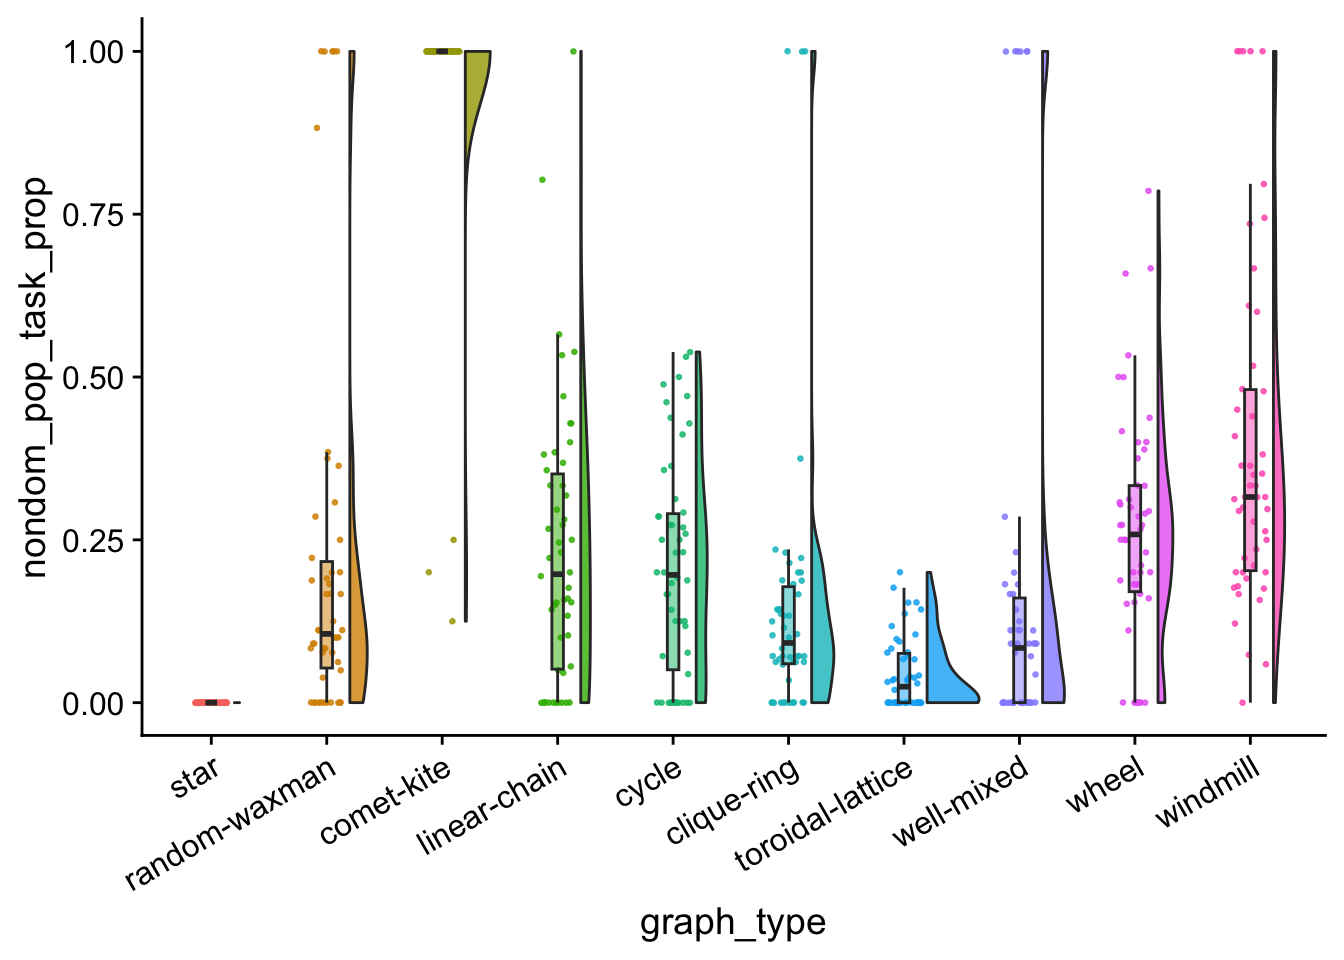
\includegraphics{supplemental-material_files/figure-latex/unnamed-chunk-55-1.pdf}

\begin{Shaded}
\begin{Highlighting}[]
\NormalTok{data }\SpecialCharTok{\%\textgreater{}\%}
  \FunctionTok{group\_by}\NormalTok{(graph\_type) }\SpecialCharTok{\%\textgreater{}\%}
  \FunctionTok{summarize}\NormalTok{(}
    \AttributeTok{reps =} \FunctionTok{n}\NormalTok{(),}
    \AttributeTok{median\_nondom\_pop\_task\_prop =} \FunctionTok{median}\NormalTok{(nondom\_pop\_task\_prop),}
    \AttributeTok{mean\_nondom\_pop\_task\_prop =} \FunctionTok{mean}\NormalTok{(nondom\_pop\_task\_prop)}
\NormalTok{  ) }\SpecialCharTok{\%\textgreater{}\%}
  \FunctionTok{arrange}\NormalTok{(}
    \FunctionTok{desc}\NormalTok{(mean\_nondom\_pop\_task\_prop)}
\NormalTok{  )}
\end{Highlighting}
\end{Shaded}

\begin{verbatim}
## # A tibble: 10 x 4
##    graph_type        reps median_nondom_pop_task_prop mean_nondom_pop_task_prop
##    <fct>            <int>                       <dbl>                     <dbl>
##  1 comet-kite          50                      1                         0.952 
##  2 windmill            50                      0.316                     0.398 
##  3 wheel               50                      0.258                     0.264 
##  4 linear-chain        50                      0.197                     0.234 
##  5 random-waxman       50                      0.106                     0.222 
##  6 cycle               50                      0.196                     0.206 
##  7 well-mixed          50                      0.0839                    0.177 
##  8 clique-ring         50                      0.0917                    0.154 
##  9 toroidal-lattice    50                      0.0245                    0.0432
## 10 star                50                      0                         0
\end{verbatim}

\begin{Shaded}
\begin{Highlighting}[]
\FunctionTok{kruskal.test}\NormalTok{(}
  \AttributeTok{formula =}\NormalTok{ nondom\_pop\_task\_prop }\SpecialCharTok{\textasciitilde{}}\NormalTok{ graph\_type,}
  \AttributeTok{data =}\NormalTok{ data}
\NormalTok{)}
\end{Highlighting}
\end{Shaded}

\begin{verbatim}
## 
##  Kruskal-Wallis rank sum test
## 
## data:  nondom_pop_task_prop by graph_type
## Kruskal-Wallis chi-squared = 256.7, df = 9, p-value < 2.2e-16
\end{verbatim}

\begin{Shaded}
\begin{Highlighting}[]
\NormalTok{wc\_results }\OtherTok{\textless{}{-}} \FunctionTok{pairwise.wilcox.test}\NormalTok{(}
  \AttributeTok{x =}\NormalTok{ data}\SpecialCharTok{$}\NormalTok{nondom\_pop\_task\_prop,}
  \AttributeTok{g =}\NormalTok{ data}\SpecialCharTok{$}\NormalTok{graph\_type,}
  \AttributeTok{p.adjust.method   =} \StringTok{"holm"}\NormalTok{,}
  \AttributeTok{exact =} \ConstantTok{FALSE}
\NormalTok{)}

\NormalTok{nondom\_pop\_task\_prop\_wc\_table }\OtherTok{\textless{}{-}} \FunctionTok{kbl}\NormalTok{(wc\_results}\SpecialCharTok{$}\NormalTok{p.value) }\SpecialCharTok{\%\textgreater{}\%} \FunctionTok{kable\_styling}\NormalTok{()}
\FunctionTok{save\_kable}\NormalTok{(nondom\_pop\_task\_prop\_wc\_table, }\FunctionTok{paste0}\NormalTok{(plot\_dir, }\StringTok{"/nondom\_pop\_task\_prop\_wc\_table.pdf"}\NormalTok{))}
\NormalTok{nondom\_pop\_task\_prop\_wc\_table}
\end{Highlighting}
\end{Shaded}

\begin{table}
\centering
\begin{tabular}[t]{l|r|r|r|r|r|r|r|r|r}
\hline
  & star & random-waxman & comet-kite & linear-chain & cycle & clique-ring & toroidal-lattice & well-mixed & wheel\\
\hline
random-waxman & 0e+00 & NA & NA & NA & NA & NA & NA & NA & NA\\
\hline
comet-kite & 0e+00 & 0.0000000 & NA & NA & NA & NA & NA & NA & NA\\
\hline
linear-chain & 0e+00 & 0.9560919 & 0 & NA & NA & NA & NA & NA & NA\\
\hline
cycle & 0e+00 & 1.0000000 & 0 & 1.0000000 & NA & NA & NA & NA & NA\\
\hline
clique-ring & 0e+00 & 1.0000000 & 0 & 0.1142983 & 0.1337364 & NA & NA & NA & NA\\
\hline
toroidal-lattice & 2e-07 & 0.0001655 & 0 & 0.0000044 & 0.0000102 & 0.0019354 & NA & NA & NA\\
\hline
well-mixed & 0e+00 & 0.4737074 & 0 & 0.0370381 & 0.0501364 & 1.0000000 & 0.4737074 & NA & NA\\
\hline
wheel & 0e+00 & 0.0560536 & 0 & 1.0000000 & 0.8350382 & 0.0002916 & 0.0000000 & 0.0003351 & NA\\
\hline
windmill & 0e+00 & 0.0000660 & 0 & 0.0129065 & 0.0022312 & 0.0000000 & 0.0000000 & 0.0000002 & 0.1337364\\
\hline
\end{tabular}
\end{table}

\begin{Shaded}
\begin{Highlighting}[]
\CommentTok{\# kruskal.test(}
\CommentTok{\#   formula = dom\_task\_total \textasciitilde{} graph\_type,}
\CommentTok{\#   data = filter(completed\_runs\_data)}
\CommentTok{\# )}
\end{Highlighting}
\end{Shaded}

\hypertarget{dominant-gestation-time}{%
\section{Dominant gestation time}\label{dominant-gestation-time}}

\begin{Shaded}
\begin{Highlighting}[]
\NormalTok{dom\_gestation\_time\_plt }\OtherTok{\textless{}{-}} \FunctionTok{ggplot}\NormalTok{(}
    \AttributeTok{data =}\NormalTok{ data,}
    \AttributeTok{mapping =} \FunctionTok{aes}\NormalTok{(}
      \AttributeTok{x =}\NormalTok{ graph\_type,}
      \AttributeTok{y =}\NormalTok{ dom\_detail\_gestation\_time,}
      \AttributeTok{fill =}\NormalTok{ graph\_type}
\NormalTok{    )}
\NormalTok{  ) }\SpecialCharTok{+}
  \FunctionTok{geom\_flat\_violin}\NormalTok{(}
    \AttributeTok{position =} \FunctionTok{position\_nudge}\NormalTok{(}\AttributeTok{x =}\NormalTok{ .}\DecValTok{2}\NormalTok{, }\AttributeTok{y =} \DecValTok{0}\NormalTok{),}
    \AttributeTok{alpha =}\NormalTok{ .}\DecValTok{8}
\NormalTok{  ) }\SpecialCharTok{+}
  \FunctionTok{geom\_point}\NormalTok{(}
    \AttributeTok{mapping=}\FunctionTok{aes}\NormalTok{(}\AttributeTok{color =}\NormalTok{ graph\_type),}
    \AttributeTok{position =} \FunctionTok{position\_jitter}\NormalTok{(}\AttributeTok{width =}\NormalTok{ .}\DecValTok{15}\NormalTok{),}
    \AttributeTok{size =}\NormalTok{ .}\DecValTok{5}\NormalTok{,}
    \AttributeTok{alpha =} \FloatTok{0.8}
\NormalTok{  ) }\SpecialCharTok{+}
  \FunctionTok{geom\_boxplot}\NormalTok{(}
    \AttributeTok{width =}\NormalTok{ .}\DecValTok{1}\NormalTok{,}
    \AttributeTok{outlier.shape =} \ConstantTok{NA}\NormalTok{,}
    \AttributeTok{alpha =} \FloatTok{0.5}
\NormalTok{  ) }\SpecialCharTok{+}
  \FunctionTok{theme}\NormalTok{(}
    \AttributeTok{legend.position =} \StringTok{"none"}\NormalTok{,}
    \AttributeTok{axis.text.x =} \FunctionTok{element\_text}\NormalTok{(}
      \AttributeTok{angle =} \DecValTok{30}\NormalTok{,}
      \AttributeTok{hjust =} \DecValTok{1}
\NormalTok{    )}
\NormalTok{  )}

\FunctionTok{ggsave}\NormalTok{(}
  \AttributeTok{filename =} \FunctionTok{paste0}\NormalTok{(plot\_dir, }\StringTok{"/dom\_gestation\_time.pdf"}\NormalTok{),}
  \AttributeTok{plot =}\NormalTok{ dom\_gestation\_time\_plt,}
  \AttributeTok{width =} \DecValTok{15}\NormalTok{,}
  \AttributeTok{height =} \DecValTok{10}
\NormalTok{)}

\NormalTok{dom\_gestation\_time\_plt}
\end{Highlighting}
\end{Shaded}

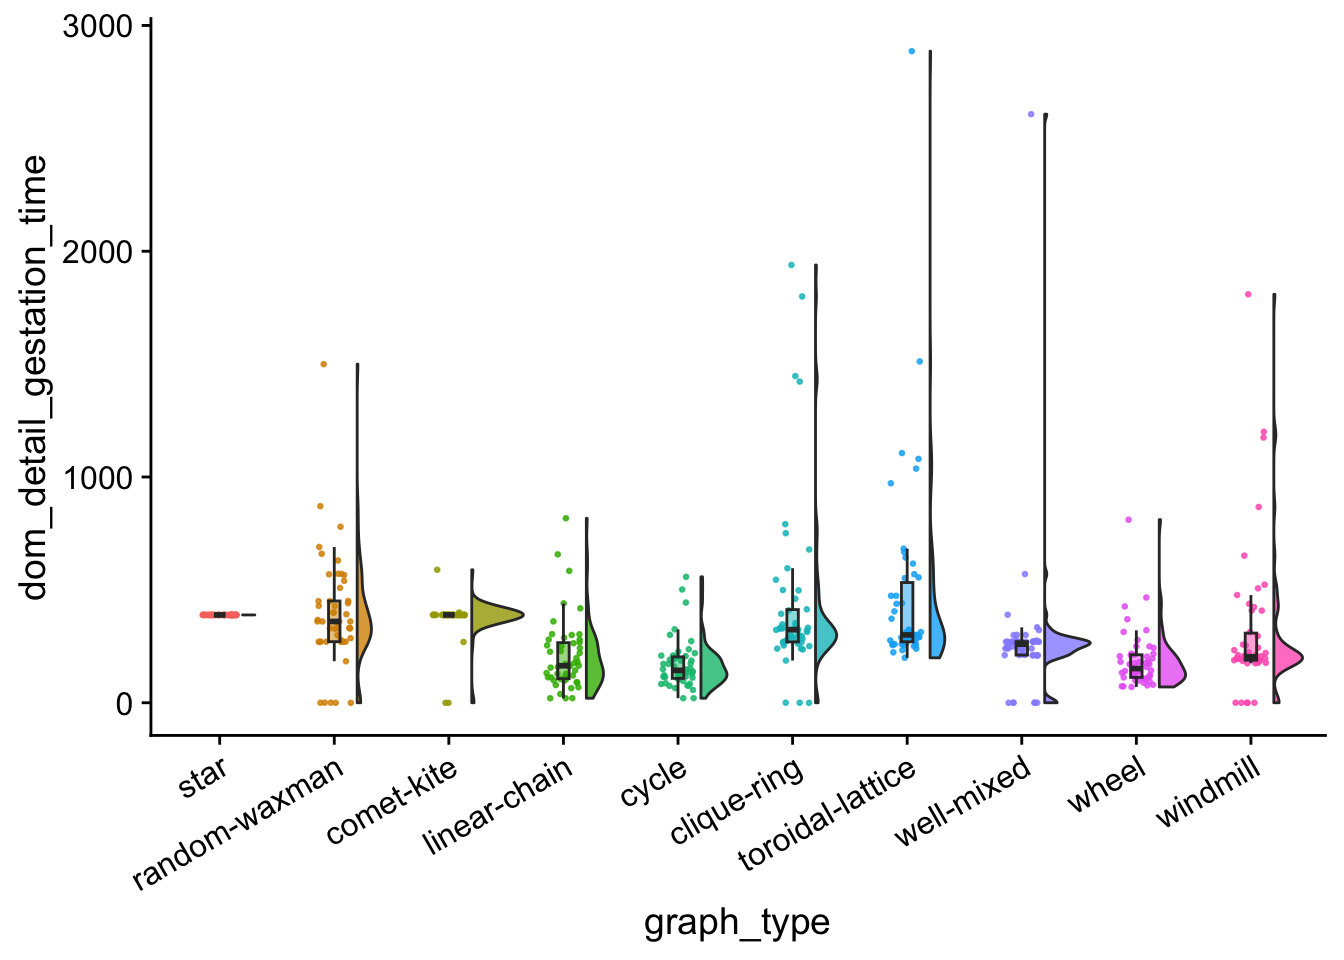
\includegraphics{supplemental-material_files/figure-latex/unnamed-chunk-59-1.pdf}

\begin{Shaded}
\begin{Highlighting}[]
\NormalTok{data }\SpecialCharTok{\%\textgreater{}\%}
  \FunctionTok{group\_by}\NormalTok{(graph\_type) }\SpecialCharTok{\%\textgreater{}\%}
  \FunctionTok{summarize}\NormalTok{(}
    \AttributeTok{reps =} \FunctionTok{n}\NormalTok{(),}
    \AttributeTok{median\_dom\_detail\_gestation\_time =} \FunctionTok{median}\NormalTok{(dom\_detail\_gestation\_time),}
    \AttributeTok{mean\_dom\_detail\_gestation\_time =} \FunctionTok{mean}\NormalTok{(dom\_detail\_gestation\_time)}
\NormalTok{  ) }\SpecialCharTok{\%\textgreater{}\%}
  \FunctionTok{arrange}\NormalTok{(}
    \FunctionTok{desc}\NormalTok{(mean\_dom\_detail\_gestation\_time)}
\NormalTok{  )}
\end{Highlighting}
\end{Shaded}

\begin{verbatim}
## # A tibble: 10 x 4
##    graph_type        reps median_dom_detail_gestation_t~1 mean_dom_detail_gest~2
##    <fct>            <int>                           <dbl>                  <dbl>
##  1 toroidal-lattice    50                            300.                   480.
##  2 clique-ring         50                            324.                   440.
##  3 random-waxman       50                            360                    393.
##  4 star                50                            389                    389 
##  5 comet-kite          50                            389                    375.
##  6 windmill            50                            204.                   315.
##  7 well-mixed          50                            260.                   281.
##  8 linear-chain        50                            164                    208.
##  9 wheel               50                            152.                   187.
## 10 cycle               50                            144.                   169.
## # i abbreviated names: 1: median_dom_detail_gestation_time,
## #   2: mean_dom_detail_gestation_time
\end{verbatim}

\begin{Shaded}
\begin{Highlighting}[]
\FunctionTok{kruskal.test}\NormalTok{(}
  \AttributeTok{formula =}\NormalTok{ dom\_detail\_gestation\_time }\SpecialCharTok{\textasciitilde{}}\NormalTok{ graph\_type,}
  \AttributeTok{data =}\NormalTok{ data}
\NormalTok{)}
\end{Highlighting}
\end{Shaded}

\begin{verbatim}
## 
##  Kruskal-Wallis rank sum test
## 
## data:  dom_detail_gestation_time by graph_type
## Kruskal-Wallis chi-squared = 197.97, df = 9, p-value < 2.2e-16
\end{verbatim}

\begin{Shaded}
\begin{Highlighting}[]
\NormalTok{wc\_results }\OtherTok{\textless{}{-}} \FunctionTok{pairwise.wilcox.test}\NormalTok{(}
  \AttributeTok{x =}\NormalTok{ data}\SpecialCharTok{$}\NormalTok{dom\_detail\_gestation\_time,}
  \AttributeTok{g =}\NormalTok{ data}\SpecialCharTok{$}\NormalTok{graph\_type,}
  \AttributeTok{p.adjust.method   =} \StringTok{"holm"}\NormalTok{,}
  \AttributeTok{exact =} \ConstantTok{FALSE}
\NormalTok{)}

\NormalTok{dom\_detail\_gestation\_time\_wc\_table }\OtherTok{\textless{}{-}} \FunctionTok{kbl}\NormalTok{(wc\_results}\SpecialCharTok{$}\NormalTok{p.value) }\SpecialCharTok{\%\textgreater{}\%} \FunctionTok{kable\_styling}\NormalTok{()}
\FunctionTok{save\_kable}\NormalTok{(dom\_detail\_gestation\_time\_wc\_table, }\FunctionTok{paste0}\NormalTok{(plot\_dir, }\StringTok{"/dom\_detail\_gestation\_time\_wc\_table.pdf"}\NormalTok{))}
\NormalTok{dom\_detail\_gestation\_time\_wc\_table}
\end{Highlighting}
\end{Shaded}

\begin{table}
\centering
\begin{tabular}[t]{l|r|r|r|r|r|r|r|r|r}
\hline
  & star & random-waxman & comet-kite & linear-chain & cycle & clique-ring & toroidal-lattice & well-mixed & wheel\\
\hline
random-waxman & 1.0000000 & NA & NA & NA & NA & NA & NA & NA & NA\\
\hline
comet-kite & 1.0000000 & 1.0000000 & NA & NA & NA & NA & NA & NA & NA\\
\hline
linear-chain & 0.0000000 & 0.0000161 & 0.0000000 & NA & NA & NA & NA & NA & NA\\
\hline
cycle & 0.0000000 & 0.0000001 & 0.0000000 & 1.0000000 & NA & NA & NA & NA & NA\\
\hline
clique-ring & 0.0039456 & 1.0000000 & 0.0375642 & 0.0000080 & 0.0000000 & NA & NA & NA & NA\\
\hline
toroidal-lattice & 0.1400273 & 1.0000000 & 0.5320337 & 0.0000001 & 0.0000000 & 1.0000000 & NA & NA & NA\\
\hline
well-mixed & 0.0000000 & 0.0000135 & 0.0000000 & 0.1875321 & 0.0000565 & 0.0001086 & 1.61e-05 & NA & NA\\
\hline
wheel & 0.0000000 & 0.0000003 & 0.0000000 & 1.0000000 & 1.0000000 & 0.0000000 & 0.00e+00 & 0.0012044 & NA\\
\hline
windmill & 0.0000430 & 0.0038095 & 0.0005370 & 0.2673588 & 0.0015818 & 0.0015818 & 4.30e-05 & 0.5320337 & 0.0088282\\
\hline
\end{tabular}
\end{table}

\hypertarget{dominant-genome-length}{%
\section{Dominant genome length}\label{dominant-genome-length}}

\begin{Shaded}
\begin{Highlighting}[]
\NormalTok{dom\_genome\_length\_plt }\OtherTok{\textless{}{-}} \FunctionTok{ggplot}\NormalTok{(}
    \AttributeTok{data =}\NormalTok{ data,}
    \AttributeTok{mapping =} \FunctionTok{aes}\NormalTok{(}
      \AttributeTok{x =}\NormalTok{ graph\_type,}
      \AttributeTok{y =}\NormalTok{ dom\_detail\_genome\_length,}
      \AttributeTok{fill =}\NormalTok{ graph\_type}
\NormalTok{    )}
\NormalTok{  ) }\SpecialCharTok{+}
  \FunctionTok{geom\_flat\_violin}\NormalTok{(}
    \AttributeTok{position =} \FunctionTok{position\_nudge}\NormalTok{(}\AttributeTok{x =}\NormalTok{ .}\DecValTok{2}\NormalTok{, }\AttributeTok{y =} \DecValTok{0}\NormalTok{),}
    \AttributeTok{alpha =}\NormalTok{ .}\DecValTok{8}
\NormalTok{  ) }\SpecialCharTok{+}
  \FunctionTok{geom\_point}\NormalTok{(}
    \AttributeTok{mapping=}\FunctionTok{aes}\NormalTok{(}\AttributeTok{color =}\NormalTok{ graph\_type),}
    \AttributeTok{position =} \FunctionTok{position\_jitter}\NormalTok{(}\AttributeTok{width =}\NormalTok{ .}\DecValTok{15}\NormalTok{),}
    \AttributeTok{size =}\NormalTok{ .}\DecValTok{5}\NormalTok{,}
    \AttributeTok{alpha =} \FloatTok{0.8}
\NormalTok{  ) }\SpecialCharTok{+}
  \FunctionTok{geom\_boxplot}\NormalTok{(}
    \AttributeTok{width =}\NormalTok{ .}\DecValTok{1}\NormalTok{,}
    \AttributeTok{outlier.shape =} \ConstantTok{NA}\NormalTok{,}
    \AttributeTok{alpha =} \FloatTok{0.5}
\NormalTok{  ) }\SpecialCharTok{+}
  \FunctionTok{theme}\NormalTok{(}
    \AttributeTok{legend.position =} \StringTok{"none"}\NormalTok{,}
    \AttributeTok{axis.text.x =} \FunctionTok{element\_text}\NormalTok{(}
      \AttributeTok{angle =} \DecValTok{30}\NormalTok{,}
      \AttributeTok{hjust =} \DecValTok{1}
\NormalTok{    )}
\NormalTok{  )}

\FunctionTok{ggsave}\NormalTok{(}
  \AttributeTok{filename =} \FunctionTok{paste0}\NormalTok{(plot\_dir, }\StringTok{"/dom\_genome\_length.pdf"}\NormalTok{),}
  \AttributeTok{plot =}\NormalTok{ dom\_genome\_length\_plt,}
  \AttributeTok{width =} \DecValTok{15}\NormalTok{,}
  \AttributeTok{height =} \DecValTok{10}
\NormalTok{)}

\NormalTok{dom\_genome\_length\_plt}
\end{Highlighting}
\end{Shaded}

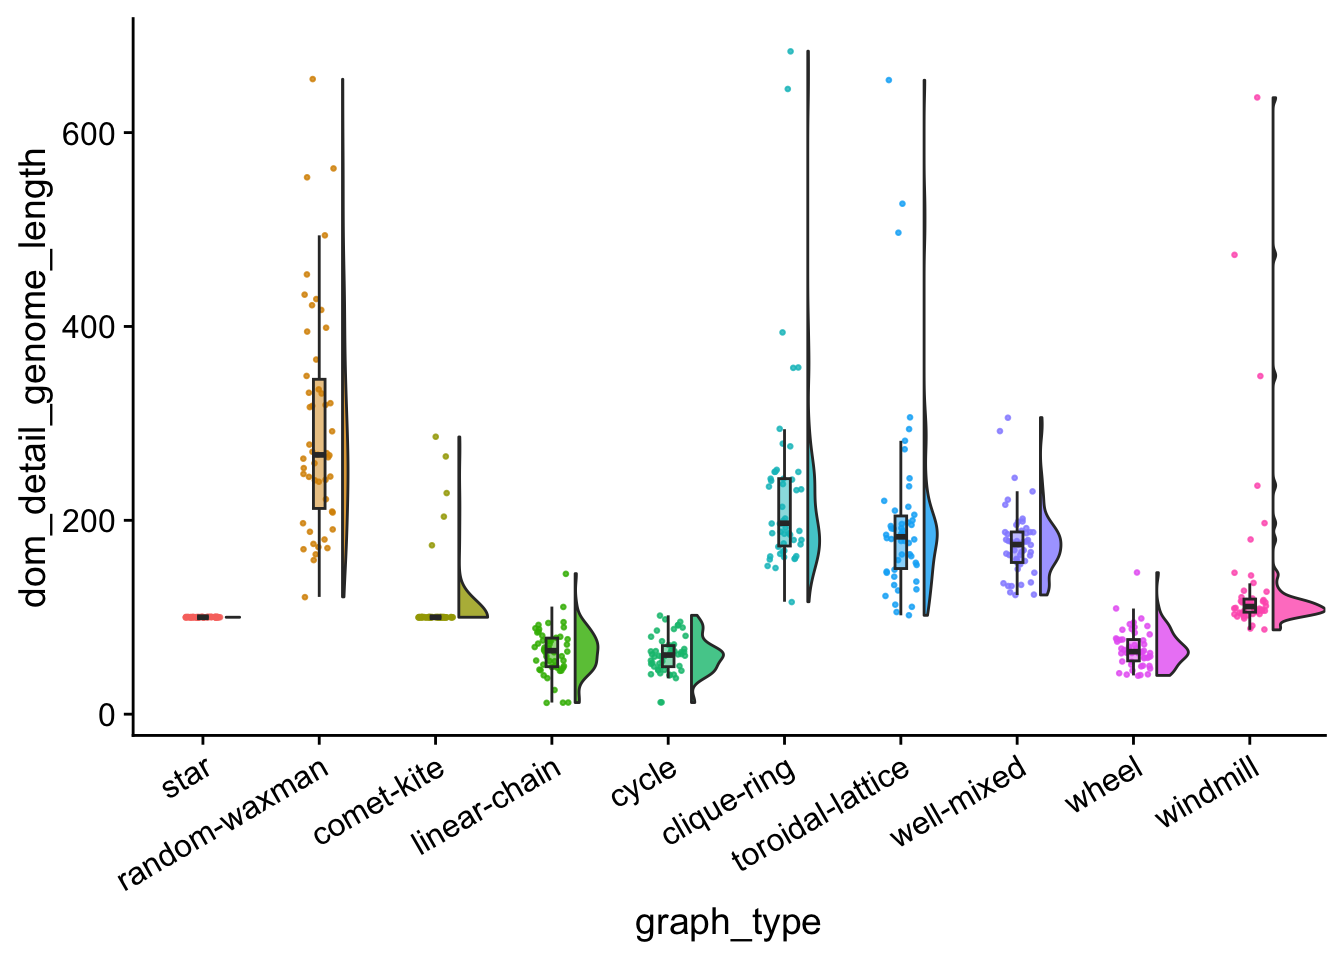
\includegraphics{supplemental-material_files/figure-latex/unnamed-chunk-62-1.pdf}

\begin{Shaded}
\begin{Highlighting}[]
\NormalTok{data }\SpecialCharTok{\%\textgreater{}\%}
  \FunctionTok{group\_by}\NormalTok{(graph\_type) }\SpecialCharTok{\%\textgreater{}\%}
  \FunctionTok{summarize}\NormalTok{(}
    \AttributeTok{reps =} \FunctionTok{n}\NormalTok{(),}
    \AttributeTok{median\_dom\_detail\_genome\_length =} \FunctionTok{median}\NormalTok{(dom\_detail\_genome\_length),}
    \AttributeTok{mean\_dom\_detail\_genome\_length =} \FunctionTok{mean}\NormalTok{(dom\_detail\_genome\_length)}
\NormalTok{  ) }\SpecialCharTok{\%\textgreater{}\%}
  \FunctionTok{arrange}\NormalTok{(}
    \FunctionTok{desc}\NormalTok{(mean\_dom\_detail\_genome\_length)}
\NormalTok{  )}
\end{Highlighting}
\end{Shaded}

\begin{verbatim}
## # A tibble: 10 x 4
##    graph_type        reps median_dom_detail_genome_length mean_dom_detail_geno~1
##    <fct>            <int>                           <dbl>                  <dbl>
##  1 random-waxman       50                           268.                   298. 
##  2 clique-ring         50                           197                    230. 
##  3 toroidal-lattice    50                           183                    203. 
##  4 well-mixed          50                           175                    177. 
##  5 windmill            50                           111                    139. 
##  6 comet-kite          50                           100                    113. 
##  7 star                50                           100                    100  
##  8 wheel               50                            64.5                   68.2
##  9 linear-chain        50                            65.5                   64.4
## 10 cycle               50                            61                     61.2
## # i abbreviated name: 1: mean_dom_detail_genome_length
\end{verbatim}

\begin{Shaded}
\begin{Highlighting}[]
\FunctionTok{kruskal.test}\NormalTok{(}
  \AttributeTok{formula =}\NormalTok{ dom\_detail\_genome\_length }\SpecialCharTok{\textasciitilde{}}\NormalTok{ graph\_type,}
  \AttributeTok{data =}\NormalTok{ data}
\NormalTok{)}
\end{Highlighting}
\end{Shaded}

\begin{verbatim}
## 
##  Kruskal-Wallis rank sum test
## 
## data:  dom_detail_genome_length by graph_type
## Kruskal-Wallis chi-squared = 423.75, df = 9, p-value < 2.2e-16
\end{verbatim}

\begin{Shaded}
\begin{Highlighting}[]
\NormalTok{wc\_results }\OtherTok{\textless{}{-}} \FunctionTok{pairwise.wilcox.test}\NormalTok{(}
  \AttributeTok{x =}\NormalTok{ data}\SpecialCharTok{$}\NormalTok{dom\_detail\_genome\_length,}
  \AttributeTok{g =}\NormalTok{ data}\SpecialCharTok{$}\NormalTok{graph\_type,}
  \AttributeTok{p.adjust.method   =} \StringTok{"holm"}\NormalTok{,}
  \AttributeTok{exact =} \ConstantTok{FALSE}
\NormalTok{)}

\NormalTok{dom\_detail\_genome\_length\_wc\_table }\OtherTok{\textless{}{-}} \FunctionTok{kbl}\NormalTok{(wc\_results}\SpecialCharTok{$}\NormalTok{p.value) }\SpecialCharTok{\%\textgreater{}\%} \FunctionTok{kable\_styling}\NormalTok{()}
\FunctionTok{save\_kable}\NormalTok{(dom\_detail\_genome\_length\_wc\_table, }\FunctionTok{paste0}\NormalTok{(plot\_dir, }\StringTok{"/dom\_detail\_genome\_length\_wc\_table.pdf"}\NormalTok{))}
\NormalTok{dom\_detail\_genome\_length\_wc\_table}
\end{Highlighting}
\end{Shaded}

\begin{table}
\centering
\begin{tabular}[t]{l|r|r|r|r|r|r|r|r|r}
\hline
  & star & random-waxman & comet-kite & linear-chain & cycle & clique-ring & toroidal-lattice & well-mixed & wheel\\
\hline
random-waxman & 0.0000000 & NA & NA & NA & NA & NA & NA & NA & NA\\
\hline
comet-kite & 0.1373564 & 0.0000000 & NA & NA & NA & NA & NA & NA & NA\\
\hline
linear-chain & 0.0000000 & 0.0000000 & 0 & NA & NA & NA & NA & NA & NA\\
\hline
cycle & 0.0000000 & 0.0000000 & 0 & 0.85562 & NA & NA & NA & NA & NA\\
\hline
clique-ring & 0.0000000 & 0.0007957 & 0 & 0.00000 & 0.0000000 & NA & NA & NA & NA\\
\hline
toroidal-lattice & 0.0000000 & 0.0000044 & 0 & 0.00000 & 0.0000000 & 0.1373564 & NA & NA & NA\\
\hline
well-mixed & 0.0000000 & 0.0000000 & 0 & 0.00000 & 0.0000000 & 0.0016198 & 0.85562 & NA & NA\\
\hline
wheel & 0.0000000 & 0.0000000 & 0 & 0.85562 & 0.4828684 & 0.0000000 & 0.00000 & 0 & NA\\
\hline
windmill & 0.0000000 & 0.0000000 & 0 & 0.00000 & 0.0000000 & 0.0000000 & 0.00000 & 0 & 0\\
\hline
\end{tabular}
\end{table}

\hypertarget{task-profile-entropy}{%
\section{Task profile entropy}\label{task-profile-entropy}}

\begin{Shaded}
\begin{Highlighting}[]
\NormalTok{task\_profile\_entropy\_plt }\OtherTok{\textless{}{-}} \FunctionTok{ggplot}\NormalTok{(}
    \AttributeTok{data =}\NormalTok{ data,}
    \AttributeTok{mapping =} \FunctionTok{aes}\NormalTok{(}
      \AttributeTok{x =}\NormalTok{ graph\_type,}
      \AttributeTok{y =}\NormalTok{ task\_profile\_entropy,}
      \AttributeTok{fill =}\NormalTok{ graph\_type}
\NormalTok{    )}
\NormalTok{  ) }\SpecialCharTok{+}
  \FunctionTok{geom\_flat\_violin}\NormalTok{(}
    \AttributeTok{position =} \FunctionTok{position\_nudge}\NormalTok{(}\AttributeTok{x =}\NormalTok{ .}\DecValTok{2}\NormalTok{, }\AttributeTok{y =} \DecValTok{0}\NormalTok{),}
    \AttributeTok{alpha =}\NormalTok{ .}\DecValTok{8}
\NormalTok{  ) }\SpecialCharTok{+}
  \FunctionTok{geom\_point}\NormalTok{(}
    \AttributeTok{mapping=}\FunctionTok{aes}\NormalTok{(}\AttributeTok{color =}\NormalTok{ graph\_type),}
    \AttributeTok{position =} \FunctionTok{position\_jitter}\NormalTok{(}\AttributeTok{width =}\NormalTok{ .}\DecValTok{15}\NormalTok{),}
    \AttributeTok{size =}\NormalTok{ .}\DecValTok{5}\NormalTok{,}
    \AttributeTok{alpha =} \FloatTok{0.8}
\NormalTok{  ) }\SpecialCharTok{+}
  \FunctionTok{geom\_boxplot}\NormalTok{(}
    \AttributeTok{width =}\NormalTok{ .}\DecValTok{1}\NormalTok{,}
    \AttributeTok{outlier.shape =} \ConstantTok{NA}\NormalTok{,}
    \AttributeTok{alpha =} \FloatTok{0.5}
\NormalTok{  ) }\SpecialCharTok{+}
  \FunctionTok{theme}\NormalTok{(}
    \AttributeTok{legend.position =} \StringTok{"none"}\NormalTok{,}
    \AttributeTok{axis.text.x =} \FunctionTok{element\_text}\NormalTok{(}
      \AttributeTok{angle =} \DecValTok{30}\NormalTok{,}
      \AttributeTok{hjust =} \DecValTok{1}
\NormalTok{    )}
\NormalTok{  )}

\FunctionTok{ggsave}\NormalTok{(}
  \AttributeTok{filename =} \FunctionTok{paste0}\NormalTok{(plot\_dir, }\StringTok{"/task\_profile\_entropy.pdf"}\NormalTok{),}
  \AttributeTok{plot =}\NormalTok{ task\_profile\_entropy\_plt,}
  \AttributeTok{width =} \DecValTok{15}\NormalTok{,}
  \AttributeTok{height =} \DecValTok{10}
\NormalTok{)}

\NormalTok{task\_profile\_entropy\_plt}
\end{Highlighting}
\end{Shaded}

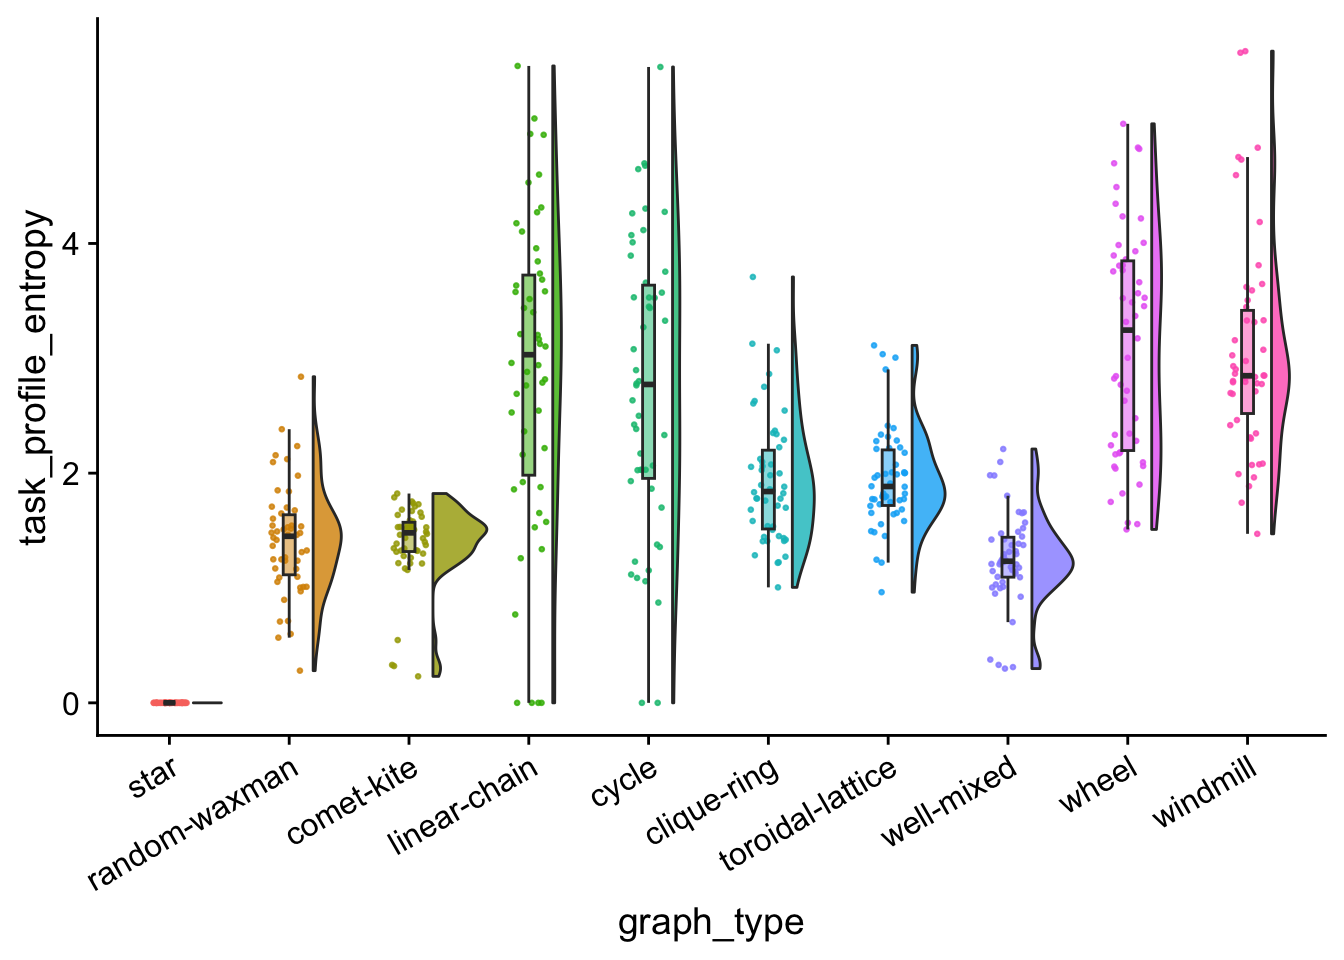
\includegraphics{supplemental-material_files/figure-latex/unnamed-chunk-65-1.pdf}

\begin{Shaded}
\begin{Highlighting}[]
\NormalTok{task\_profile\_count\_plt }\OtherTok{\textless{}{-}} \FunctionTok{ggplot}\NormalTok{(}
    \AttributeTok{data =}\NormalTok{ data,}
    \AttributeTok{mapping =} \FunctionTok{aes}\NormalTok{(}
      \AttributeTok{x =}\NormalTok{ graph\_type,}
      \AttributeTok{y =}\NormalTok{ task\_profile\_count,}
      \AttributeTok{fill =}\NormalTok{ graph\_type}
\NormalTok{    )}
\NormalTok{  ) }\SpecialCharTok{+}
  \FunctionTok{geom\_flat\_violin}\NormalTok{(}
    \AttributeTok{position =} \FunctionTok{position\_nudge}\NormalTok{(}\AttributeTok{x =}\NormalTok{ .}\DecValTok{2}\NormalTok{, }\AttributeTok{y =} \DecValTok{0}\NormalTok{),}
    \AttributeTok{alpha =}\NormalTok{ .}\DecValTok{8}
\NormalTok{  ) }\SpecialCharTok{+}
  \FunctionTok{geom\_point}\NormalTok{(}
    \AttributeTok{mapping=}\FunctionTok{aes}\NormalTok{(}\AttributeTok{color =}\NormalTok{ graph\_type),}
    \AttributeTok{position =} \FunctionTok{position\_jitter}\NormalTok{(}\AttributeTok{width =}\NormalTok{ .}\DecValTok{15}\NormalTok{),}
    \AttributeTok{size =}\NormalTok{ .}\DecValTok{5}\NormalTok{,}
    \AttributeTok{alpha =} \FloatTok{0.8}
\NormalTok{  ) }\SpecialCharTok{+}
  \FunctionTok{geom\_boxplot}\NormalTok{(}
    \AttributeTok{width =}\NormalTok{ .}\DecValTok{1}\NormalTok{,}
    \AttributeTok{outlier.shape =} \ConstantTok{NA}\NormalTok{,}
    \AttributeTok{alpha =} \FloatTok{0.5}
\NormalTok{  ) }\SpecialCharTok{+}
  \FunctionTok{theme}\NormalTok{(}
    \AttributeTok{legend.position =} \StringTok{"none"}\NormalTok{,}
    \AttributeTok{axis.text.x =} \FunctionTok{element\_text}\NormalTok{(}
      \AttributeTok{angle =} \DecValTok{30}\NormalTok{,}
      \AttributeTok{hjust =} \DecValTok{1}
\NormalTok{    )}
\NormalTok{  )}

\FunctionTok{ggsave}\NormalTok{(}
  \AttributeTok{filename =} \FunctionTok{paste0}\NormalTok{(plot\_dir, }\StringTok{"/task\_profile\_count.pdf"}\NormalTok{),}
  \AttributeTok{plot =}\NormalTok{ task\_profile\_count\_plt,}
  \AttributeTok{width =} \DecValTok{15}\NormalTok{,}
  \AttributeTok{height =} \DecValTok{10}
\NormalTok{)}

\NormalTok{task\_profile\_count\_plt}
\end{Highlighting}
\end{Shaded}

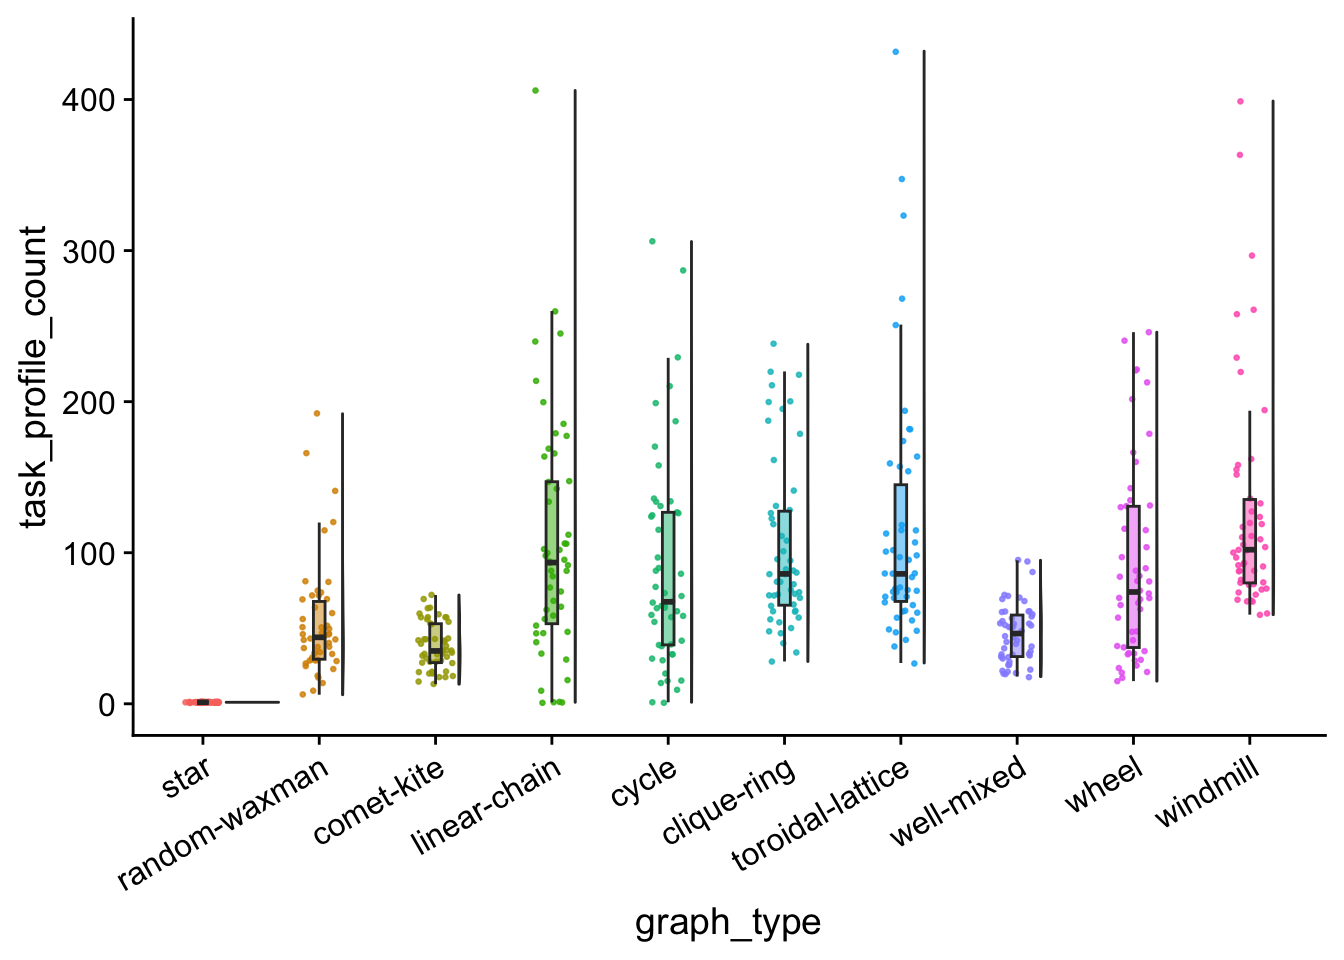
\includegraphics{supplemental-material_files/figure-latex/unnamed-chunk-66-1.pdf}

\hypertarget{average-generation}{%
\section{Average generation}\label{average-generation}}

\begin{Shaded}
\begin{Highlighting}[]
\NormalTok{avg\_generation\_plt }\OtherTok{\textless{}{-}} \FunctionTok{ggplot}\NormalTok{(}
    \AttributeTok{data =}\NormalTok{ data,}
    \AttributeTok{mapping =} \FunctionTok{aes}\NormalTok{(}
      \AttributeTok{x =}\NormalTok{ graph\_type,}
      \AttributeTok{y =}\NormalTok{ time\_average\_generation,}
      \AttributeTok{fill =}\NormalTok{ graph\_type}
\NormalTok{    )}
\NormalTok{  ) }\SpecialCharTok{+}
  \FunctionTok{geom\_flat\_violin}\NormalTok{(}
    \AttributeTok{position =} \FunctionTok{position\_nudge}\NormalTok{(}\AttributeTok{x =}\NormalTok{ .}\DecValTok{2}\NormalTok{, }\AttributeTok{y =} \DecValTok{0}\NormalTok{),}
    \AttributeTok{alpha =}\NormalTok{ .}\DecValTok{8}
\NormalTok{  ) }\SpecialCharTok{+}
  \FunctionTok{geom\_point}\NormalTok{(}
    \AttributeTok{mapping=}\FunctionTok{aes}\NormalTok{(}\AttributeTok{color =}\NormalTok{ graph\_type),}
    \AttributeTok{position =} \FunctionTok{position\_jitter}\NormalTok{(}\AttributeTok{width =}\NormalTok{ .}\DecValTok{15}\NormalTok{),}
    \AttributeTok{size =}\NormalTok{ .}\DecValTok{5}\NormalTok{,}
    \AttributeTok{alpha =} \FloatTok{0.8}
\NormalTok{  ) }\SpecialCharTok{+}
  \FunctionTok{geom\_boxplot}\NormalTok{(}
    \AttributeTok{width =}\NormalTok{ .}\DecValTok{1}\NormalTok{,}
    \AttributeTok{outlier.shape =} \ConstantTok{NA}\NormalTok{,}
    \AttributeTok{alpha =} \FloatTok{0.5}
\NormalTok{  ) }\SpecialCharTok{+}
  \FunctionTok{theme}\NormalTok{(}
    \AttributeTok{legend.position =} \StringTok{"none"}\NormalTok{,}
    \AttributeTok{axis.text.x =} \FunctionTok{element\_text}\NormalTok{(}
      \AttributeTok{angle =} \DecValTok{30}\NormalTok{,}
      \AttributeTok{hjust =} \DecValTok{1}
\NormalTok{    )}
\NormalTok{  )}

\FunctionTok{ggsave}\NormalTok{(}
  \AttributeTok{filename =} \FunctionTok{paste0}\NormalTok{(plot\_dir, }\StringTok{"/avg\_generation.pdf"}\NormalTok{),}
  \AttributeTok{plot =}\NormalTok{ avg\_generation\_plt,}
  \AttributeTok{width =} \DecValTok{15}\NormalTok{,}
  \AttributeTok{height =} \DecValTok{10}
\NormalTok{)}

\NormalTok{avg\_generation\_plt}
\end{Highlighting}
\end{Shaded}

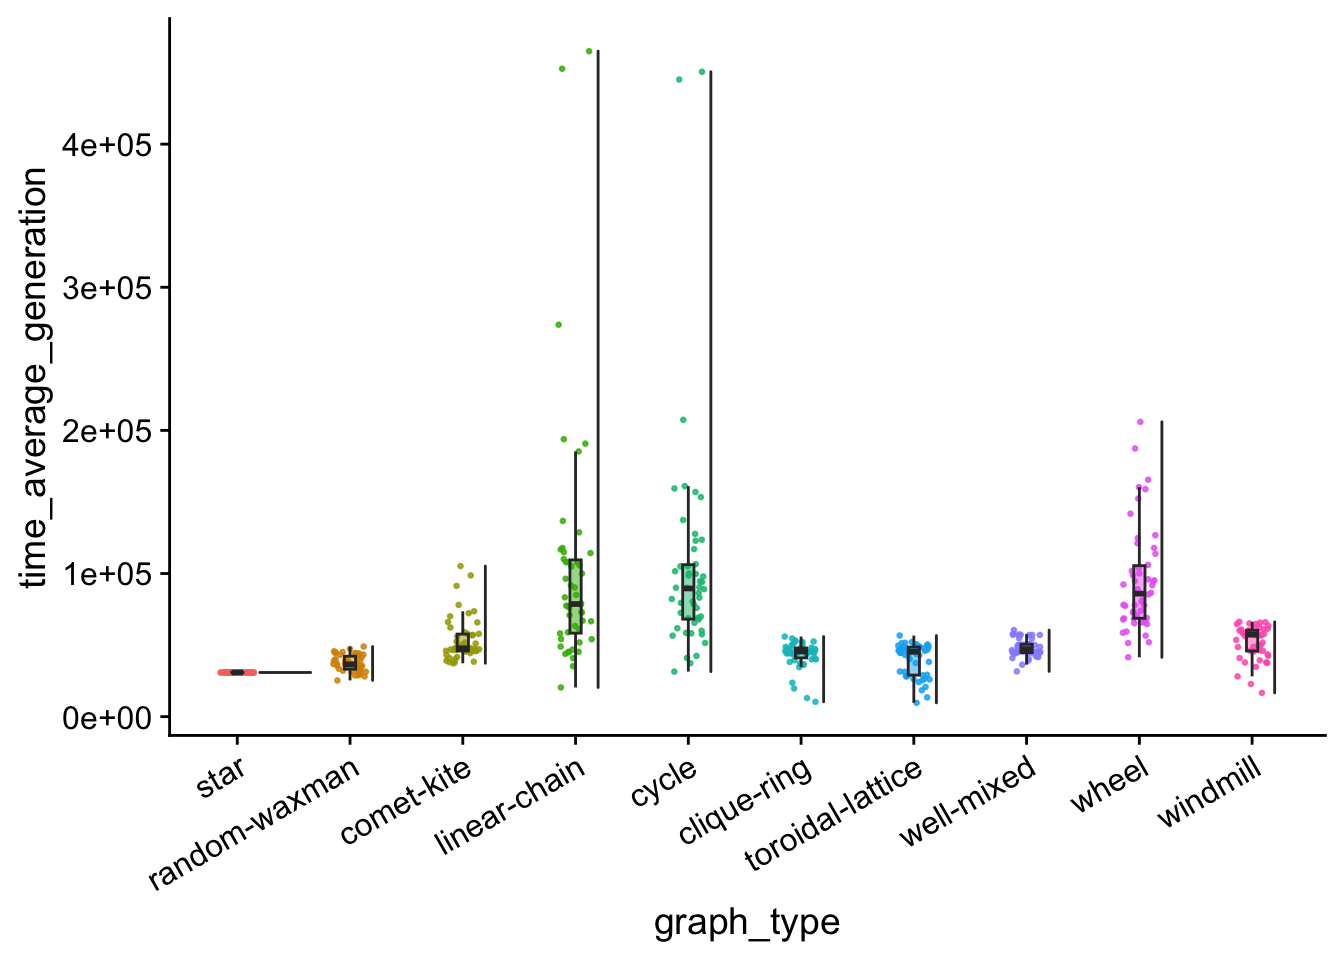
\includegraphics{supplemental-material_files/figure-latex/unnamed-chunk-67-1.pdf}

\hypertarget{population-task-count-over-time}{%
\section{Population task count over time}\label{population-task-count-over-time}}

\begin{Shaded}
\begin{Highlighting}[]
\NormalTok{pop\_task\_cnt\_ts }\OtherTok{\textless{}{-}} \FunctionTok{ggplot}\NormalTok{(}
    \AttributeTok{data =}\NormalTok{ time\_series\_data,}
    \AttributeTok{mapping =} \FunctionTok{aes}\NormalTok{(}
      \AttributeTok{x =}\NormalTok{ update,}
      \AttributeTok{y =}\NormalTok{ pop\_task\_total\_tasks\_done,}
      \AttributeTok{color =}\NormalTok{ graph\_type,}
      \AttributeTok{fill =}\NormalTok{ graph\_type}
\NormalTok{    )}
\NormalTok{  ) }\SpecialCharTok{+}
  \FunctionTok{stat\_summary}\NormalTok{(}\AttributeTok{fun =} \StringTok{"mean"}\NormalTok{, }\AttributeTok{geom =} \StringTok{"line"}\NormalTok{) }\SpecialCharTok{+}
  \FunctionTok{stat\_summary}\NormalTok{(}
    \AttributeTok{fun.data =} \StringTok{"mean\_cl\_boot"}\NormalTok{,}
    \AttributeTok{fun.args =} \FunctionTok{list}\NormalTok{(}\AttributeTok{conf.int =} \FloatTok{0.95}\NormalTok{),}
    \AttributeTok{geom =} \StringTok{"ribbon"}\NormalTok{,}
    \AttributeTok{alpha =} \FloatTok{0.2}\NormalTok{,}
    \AttributeTok{linetype =} \DecValTok{0}
\NormalTok{  ) }\SpecialCharTok{+}
  \FunctionTok{theme}\NormalTok{(}\AttributeTok{legend.position =} \StringTok{"bottom"}\NormalTok{)}

\FunctionTok{ggsave}\NormalTok{(}
  \AttributeTok{plot =}\NormalTok{ pop\_task\_cnt\_ts,}
  \AttributeTok{filename =} \FunctionTok{paste0}\NormalTok{(}
\NormalTok{    working\_directory,}
    \StringTok{"/plots/pop\_tasks\_ts.pdf"}
\NormalTok{  ),}
  \AttributeTok{width =} \DecValTok{15}\NormalTok{,}
  \AttributeTok{height =} \DecValTok{10}
\NormalTok{)}

\NormalTok{pop\_task\_cnt\_ts}
\end{Highlighting}
\end{Shaded}

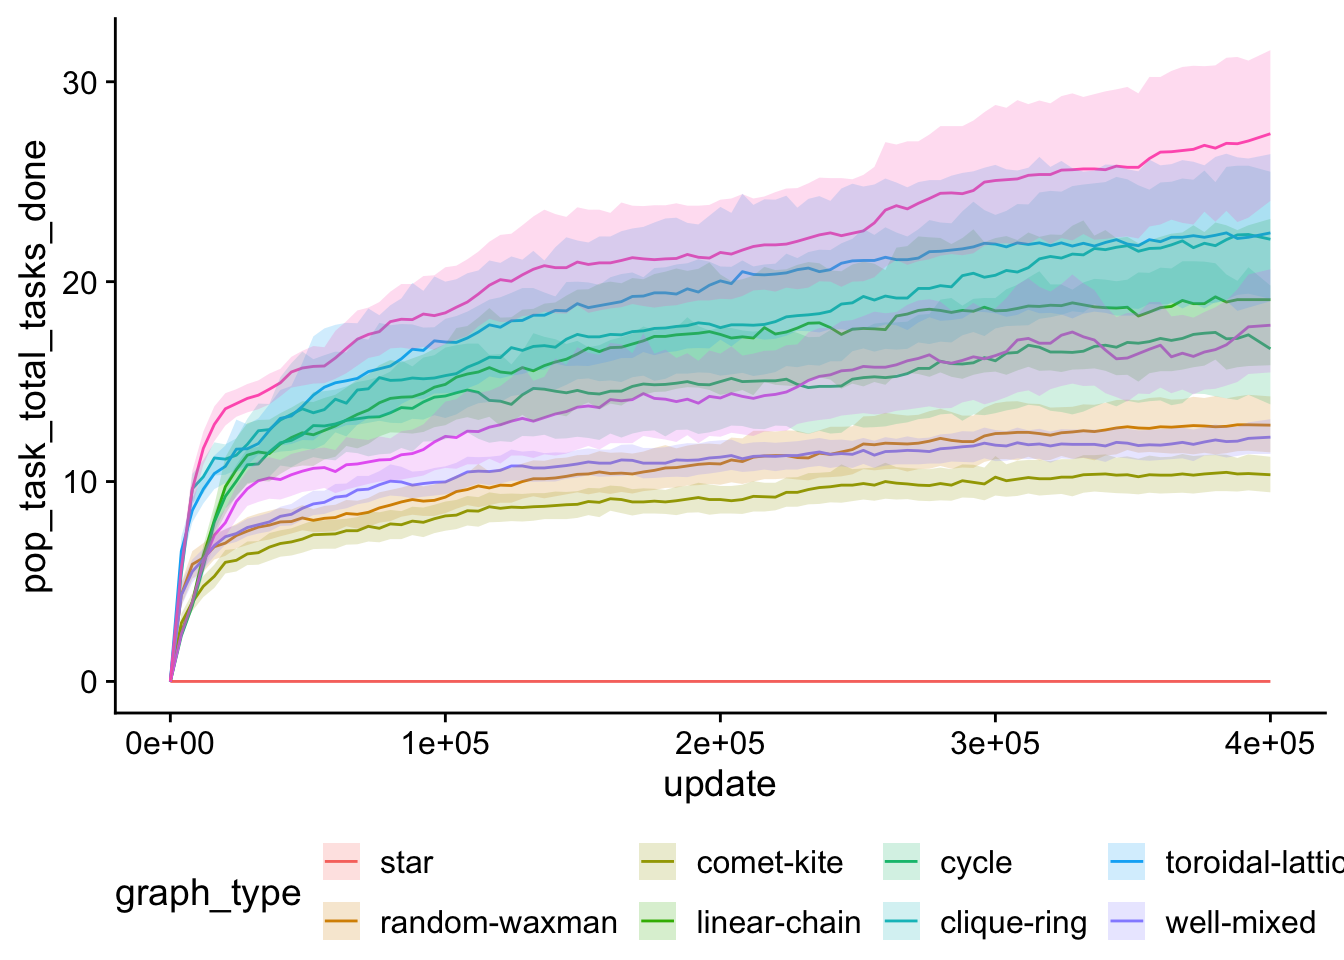
\includegraphics{supplemental-material_files/figure-latex/unnamed-chunk-68-1.pdf}

\hypertarget{average-generation-over-time}{%
\section{Average generation over time}\label{average-generation-over-time}}

\begin{Shaded}
\begin{Highlighting}[]
\NormalTok{time\_average\_generation\_ts }\OtherTok{\textless{}{-}} \FunctionTok{ggplot}\NormalTok{(}
    \AttributeTok{data =}\NormalTok{ time\_series\_data,}
    \AttributeTok{mapping =} \FunctionTok{aes}\NormalTok{(}
      \AttributeTok{x =}\NormalTok{ update,}
      \AttributeTok{y =}\NormalTok{ time\_average\_generation,}
      \AttributeTok{color =}\NormalTok{ graph\_type,}
      \AttributeTok{fill =}\NormalTok{ graph\_type}
\NormalTok{    )}
\NormalTok{  ) }\SpecialCharTok{+}
  \FunctionTok{stat\_summary}\NormalTok{(}\AttributeTok{fun =} \StringTok{"mean"}\NormalTok{, }\AttributeTok{geom =} \StringTok{"line"}\NormalTok{) }\SpecialCharTok{+}
  \FunctionTok{stat\_summary}\NormalTok{(}
    \AttributeTok{fun.data =} \StringTok{"mean\_cl\_boot"}\NormalTok{,}
    \AttributeTok{fun.args =} \FunctionTok{list}\NormalTok{(}\AttributeTok{conf.int =} \FloatTok{0.95}\NormalTok{),}
    \AttributeTok{geom =} \StringTok{"ribbon"}\NormalTok{,}
    \AttributeTok{alpha =} \FloatTok{0.2}\NormalTok{,}
    \AttributeTok{linetype =} \DecValTok{0}
\NormalTok{  ) }\SpecialCharTok{+}
  \FunctionTok{facet\_wrap}\NormalTok{(}\SpecialCharTok{\textasciitilde{}}\NormalTok{ENVIRONMENT\_FILE) }\SpecialCharTok{+}
  \FunctionTok{theme}\NormalTok{(}\AttributeTok{legend.position =} \StringTok{"bottom"}\NormalTok{)}

\FunctionTok{ggsave}\NormalTok{(}
  \AttributeTok{plot =}\NormalTok{ time\_average\_generation\_ts,}
  \AttributeTok{filename =} \FunctionTok{paste0}\NormalTok{(}
\NormalTok{    working\_directory,}
    \StringTok{"/plots/time\_average\_generation\_ts.pdf"}
\NormalTok{  ),}
  \AttributeTok{width =} \DecValTok{15}\NormalTok{,}
  \AttributeTok{height =} \DecValTok{10}
\NormalTok{)}

\NormalTok{time\_average\_generation\_ts}
\end{Highlighting}
\end{Shaded}

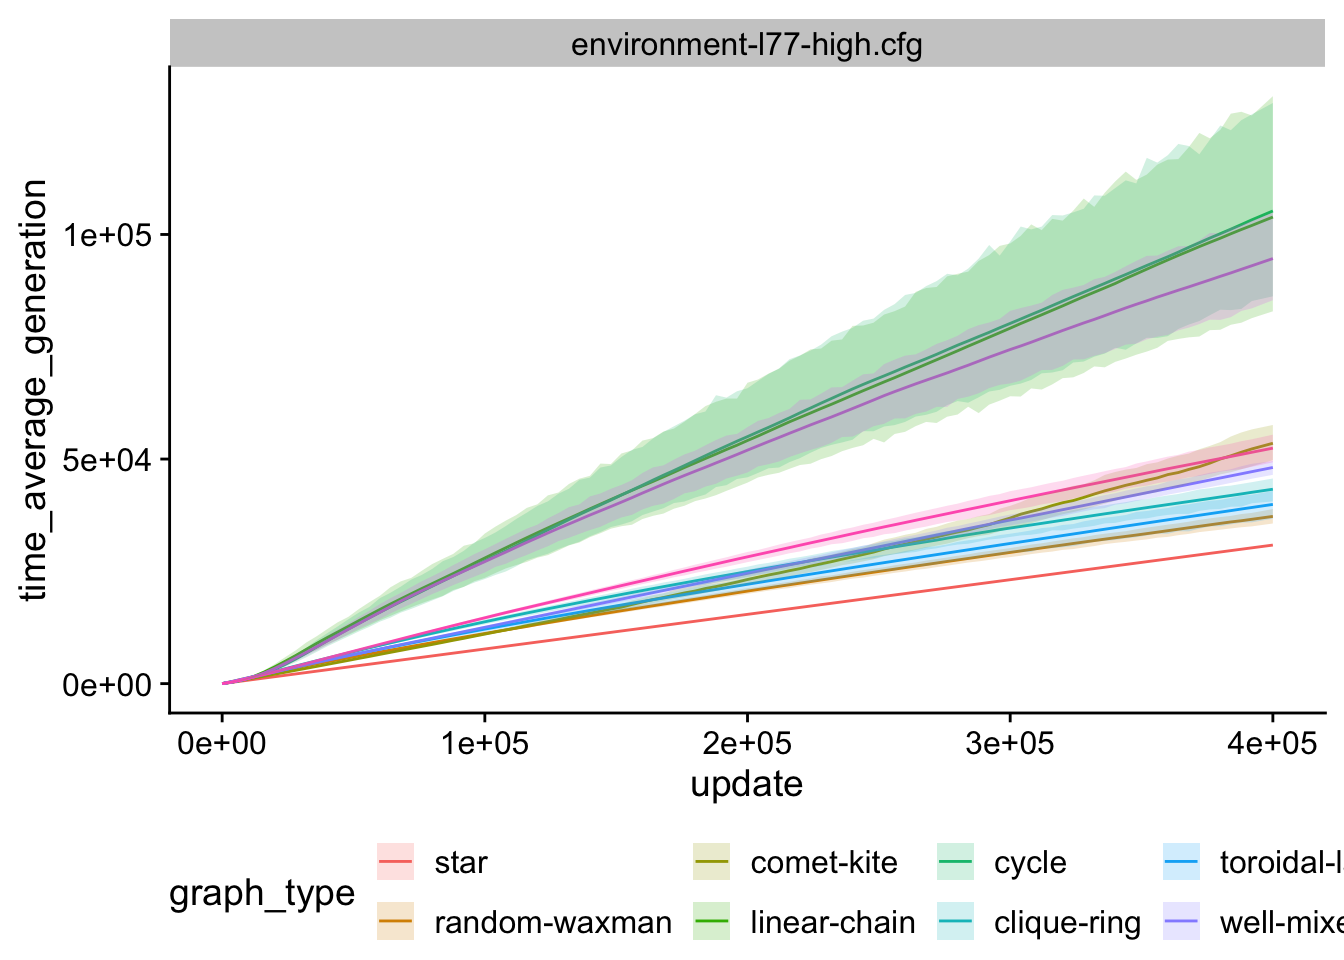
\includegraphics{supplemental-material_files/figure-latex/unnamed-chunk-69-1.pdf}

\hypertarget{graph-location-info}{%
\section{Graph location info}\label{graph-location-info}}

Analyze graph\_birth\_info\_annotated.csv

\begin{Shaded}
\begin{Highlighting}[]
\CommentTok{\# Load summary data from final update}
\NormalTok{graph\_loc\_data\_path }\OtherTok{\textless{}{-}} \FunctionTok{paste}\NormalTok{(}
\NormalTok{  working\_directory,}
  \StringTok{"data"}\NormalTok{,}
  \StringTok{"graph\_birth\_info\_annotated.csv"}\NormalTok{,}
  \AttributeTok{sep =} \StringTok{"/"}
\NormalTok{)}
\NormalTok{graph\_loc\_data }\OtherTok{\textless{}{-}} \FunctionTok{read\_csv}\NormalTok{(graph\_loc\_data\_path)}

\NormalTok{graph\_loc\_data }\OtherTok{\textless{}{-}}\NormalTok{ graph\_loc\_data }\SpecialCharTok{\%\textgreater{}\%}
  \FunctionTok{mutate}\NormalTok{(}
    \AttributeTok{graph\_type =} \FunctionTok{factor}\NormalTok{(}
\NormalTok{      graph\_type,}
      \AttributeTok{levels =} \FunctionTok{c}\NormalTok{(}
        \StringTok{"star"}\NormalTok{,}
        \StringTok{"random{-}waxman"}\NormalTok{,}
        \StringTok{"comet{-}kite"}\NormalTok{,}
        \StringTok{"linear{-}chain"}\NormalTok{,}
        \StringTok{"cycle"}\NormalTok{,}
        \StringTok{"clique{-}ring"}\NormalTok{,}
        \StringTok{"toroidal{-}lattice"}\NormalTok{,}
        \StringTok{"well{-}mixed"}\NormalTok{,}
        \StringTok{"wheel"}\NormalTok{,}
        \StringTok{"windmill"}
\NormalTok{      )}
\NormalTok{    ),}
    \AttributeTok{seed =} \FunctionTok{as.factor}\NormalTok{(seed)}
\NormalTok{  ) }\SpecialCharTok{\%\textgreater{}\%}
  \FunctionTok{filter}\NormalTok{(}
\NormalTok{    graph\_type }\SpecialCharTok{\%in\%}\NormalTok{ focal\_graphs}
\NormalTok{  )}
\end{Highlighting}
\end{Shaded}

Summarize by seed

\begin{Shaded}
\begin{Highlighting}[]
\NormalTok{graph\_loc\_data\_summary }\OtherTok{\textless{}{-}}\NormalTok{ graph\_loc\_data }\SpecialCharTok{\%\textgreater{}\%}
  \FunctionTok{group\_by}\NormalTok{(seed, graph\_type) }\SpecialCharTok{\%\textgreater{}\%}
  \FunctionTok{summarize}\NormalTok{(}
    \AttributeTok{births\_var =} \FunctionTok{var}\NormalTok{(births),}
    \AttributeTok{births\_total =} \FunctionTok{sum}\NormalTok{(births),}
    \AttributeTok{task\_apps\_total =} \FunctionTok{sum}\NormalTok{(task\_appearances),}
    \AttributeTok{task\_apps\_var =} \FunctionTok{var}\NormalTok{(task\_appearances)}
\NormalTok{  ) }\SpecialCharTok{\%\textgreater{}\%}
  \FunctionTok{ungroup}\NormalTok{()}
\end{Highlighting}
\end{Shaded}

\hypertarget{total-birth-counts}{%
\subsection{Total birth Counts}\label{total-birth-counts}}

\begin{Shaded}
\begin{Highlighting}[]
\NormalTok{birth\_counts\_total\_plt }\OtherTok{\textless{}{-}} \FunctionTok{ggplot}\NormalTok{(}
    \AttributeTok{data =}\NormalTok{ graph\_loc\_data\_summary,}
    \AttributeTok{mapping =} \FunctionTok{aes}\NormalTok{(}
      \AttributeTok{x =}\NormalTok{ graph\_type,}
      \AttributeTok{y =}\NormalTok{ births\_total,}
      \AttributeTok{fill =}\NormalTok{ graph\_type}
\NormalTok{    )}
\NormalTok{  ) }\SpecialCharTok{+}
  \FunctionTok{geom\_flat\_violin}\NormalTok{(}
    \AttributeTok{position =} \FunctionTok{position\_nudge}\NormalTok{(}\AttributeTok{x =}\NormalTok{ .}\DecValTok{2}\NormalTok{, }\AttributeTok{y =} \DecValTok{0}\NormalTok{),}
    \AttributeTok{alpha =}\NormalTok{ .}\DecValTok{8}
\NormalTok{  ) }\SpecialCharTok{+}
  \FunctionTok{geom\_point}\NormalTok{(}
    \AttributeTok{mapping=}\FunctionTok{aes}\NormalTok{(}\AttributeTok{color =}\NormalTok{ graph\_type),}
    \AttributeTok{position =} \FunctionTok{position\_jitter}\NormalTok{(}\AttributeTok{width =}\NormalTok{ .}\DecValTok{15}\NormalTok{),}
    \AttributeTok{size =}\NormalTok{ .}\DecValTok{5}\NormalTok{,}
    \AttributeTok{alpha =} \FloatTok{0.8}
\NormalTok{  ) }\SpecialCharTok{+}
  \FunctionTok{geom\_boxplot}\NormalTok{(}
    \AttributeTok{width =}\NormalTok{ .}\DecValTok{1}\NormalTok{,}
    \AttributeTok{outlier.shape =} \ConstantTok{NA}\NormalTok{,}
    \AttributeTok{alpha =} \FloatTok{0.5}
\NormalTok{  ) }\SpecialCharTok{+}
  \FunctionTok{theme}\NormalTok{(}
    \AttributeTok{legend.position =} \StringTok{"none"}\NormalTok{,}
    \AttributeTok{axis.text.x =} \FunctionTok{element\_text}\NormalTok{(}
      \AttributeTok{angle =} \DecValTok{30}\NormalTok{,}
      \AttributeTok{hjust =} \DecValTok{1}
\NormalTok{    )}
\NormalTok{  )}

\FunctionTok{ggsave}\NormalTok{(}
  \AttributeTok{filename =} \FunctionTok{paste0}\NormalTok{(plot\_dir, }\StringTok{"/birth\_counts\_total.pdf"}\NormalTok{),}
  \AttributeTok{plot =}\NormalTok{ birth\_counts\_total\_plt,}
  \AttributeTok{width =} \DecValTok{15}\NormalTok{,}
  \AttributeTok{height =} \DecValTok{10}
\NormalTok{)}

\NormalTok{birth\_counts\_total\_plt}
\end{Highlighting}
\end{Shaded}

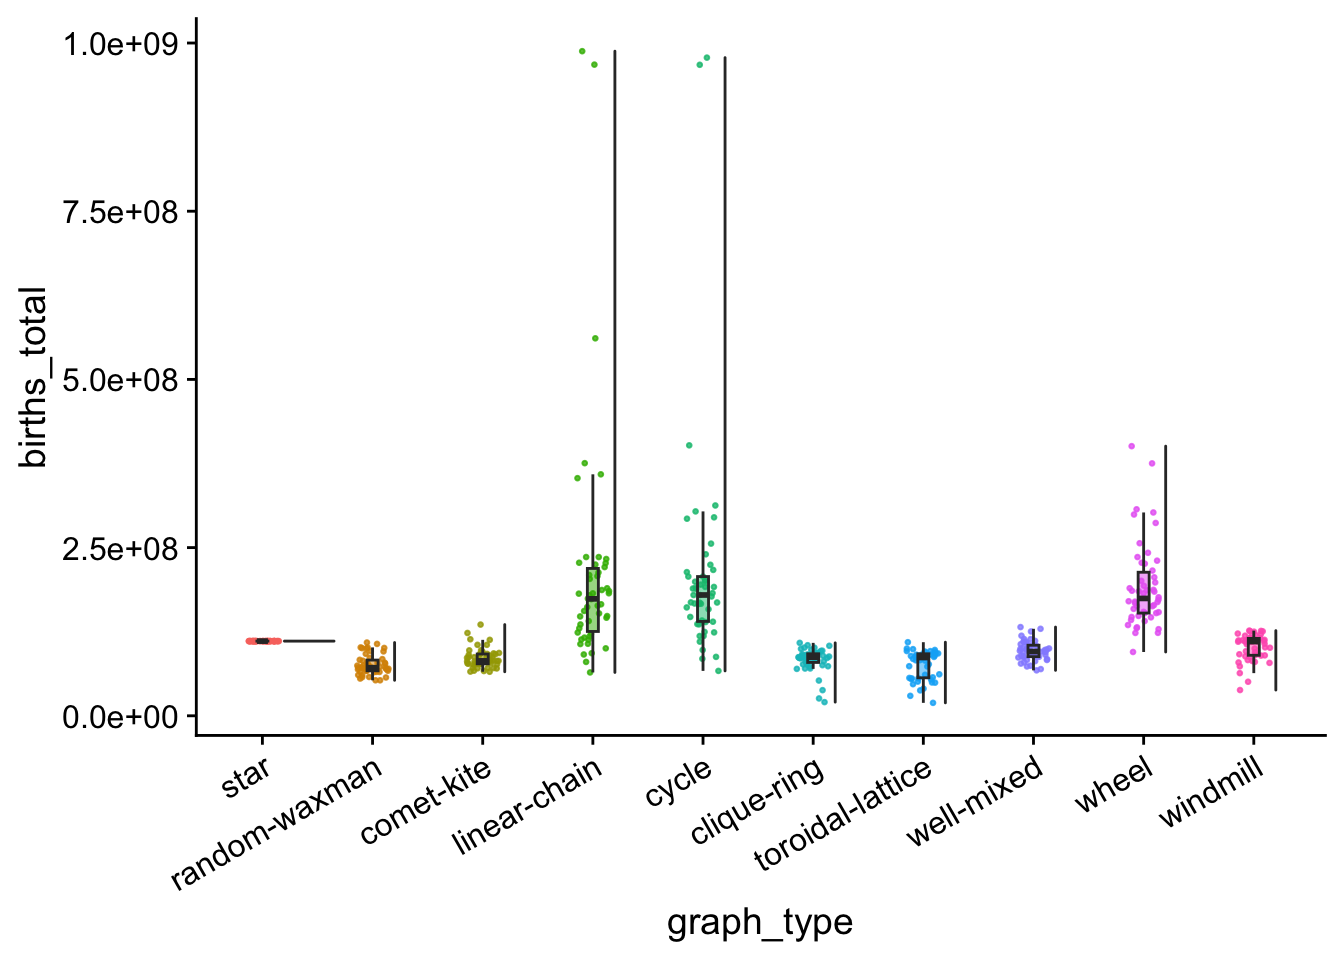
\includegraphics{supplemental-material_files/figure-latex/unnamed-chunk-72-1.pdf}

\hypertarget{variance-birth-counts}{%
\subsection{Variance birth Counts}\label{variance-birth-counts}}

\begin{Shaded}
\begin{Highlighting}[]
\NormalTok{birth\_counts\_var\_plt }\OtherTok{\textless{}{-}} \FunctionTok{ggplot}\NormalTok{(}
    \AttributeTok{data =}\NormalTok{ graph\_loc\_data\_summary,}
    \AttributeTok{mapping =} \FunctionTok{aes}\NormalTok{(}
      \AttributeTok{x =}\NormalTok{ graph\_type,}
      \AttributeTok{y =}\NormalTok{ births\_var,}
      \AttributeTok{fill =}\NormalTok{ graph\_type}
\NormalTok{    )}
\NormalTok{  ) }\SpecialCharTok{+}
  \FunctionTok{geom\_flat\_violin}\NormalTok{(}
    \AttributeTok{position =} \FunctionTok{position\_nudge}\NormalTok{(}\AttributeTok{x =}\NormalTok{ .}\DecValTok{2}\NormalTok{, }\AttributeTok{y =} \DecValTok{0}\NormalTok{),}
    \AttributeTok{alpha =}\NormalTok{ .}\DecValTok{8}
\NormalTok{  ) }\SpecialCharTok{+}
  \FunctionTok{geom\_point}\NormalTok{(}
    \AttributeTok{mapping=}\FunctionTok{aes}\NormalTok{(}\AttributeTok{color =}\NormalTok{ graph\_type),}
    \AttributeTok{position =} \FunctionTok{position\_jitter}\NormalTok{(}\AttributeTok{width =}\NormalTok{ .}\DecValTok{15}\NormalTok{),}
    \AttributeTok{size =}\NormalTok{ .}\DecValTok{5}\NormalTok{,}
    \AttributeTok{alpha =} \FloatTok{0.8}
\NormalTok{  ) }\SpecialCharTok{+}
  \FunctionTok{geom\_boxplot}\NormalTok{(}
    \AttributeTok{width =}\NormalTok{ .}\DecValTok{1}\NormalTok{,}
    \AttributeTok{outlier.shape =} \ConstantTok{NA}\NormalTok{,}
    \AttributeTok{alpha =} \FloatTok{0.5}
\NormalTok{  ) }\SpecialCharTok{+}
  \FunctionTok{theme}\NormalTok{(}
    \AttributeTok{legend.position =} \StringTok{"none"}\NormalTok{,}
    \AttributeTok{axis.text.x =} \FunctionTok{element\_text}\NormalTok{(}
      \AttributeTok{angle =} \DecValTok{30}\NormalTok{,}
      \AttributeTok{hjust =} \DecValTok{1}
\NormalTok{    )}
\NormalTok{  )}

\FunctionTok{ggsave}\NormalTok{(}
  \AttributeTok{filename =} \FunctionTok{paste0}\NormalTok{(plot\_dir, }\StringTok{"/birth\_counts\_var.pdf"}\NormalTok{),}
  \AttributeTok{plot =}\NormalTok{ birth\_counts\_var\_plt,}
  \AttributeTok{width =} \DecValTok{15}\NormalTok{,}
  \AttributeTok{height =} \DecValTok{10}
\NormalTok{)}

\NormalTok{birth\_counts\_var\_plt}
\end{Highlighting}
\end{Shaded}

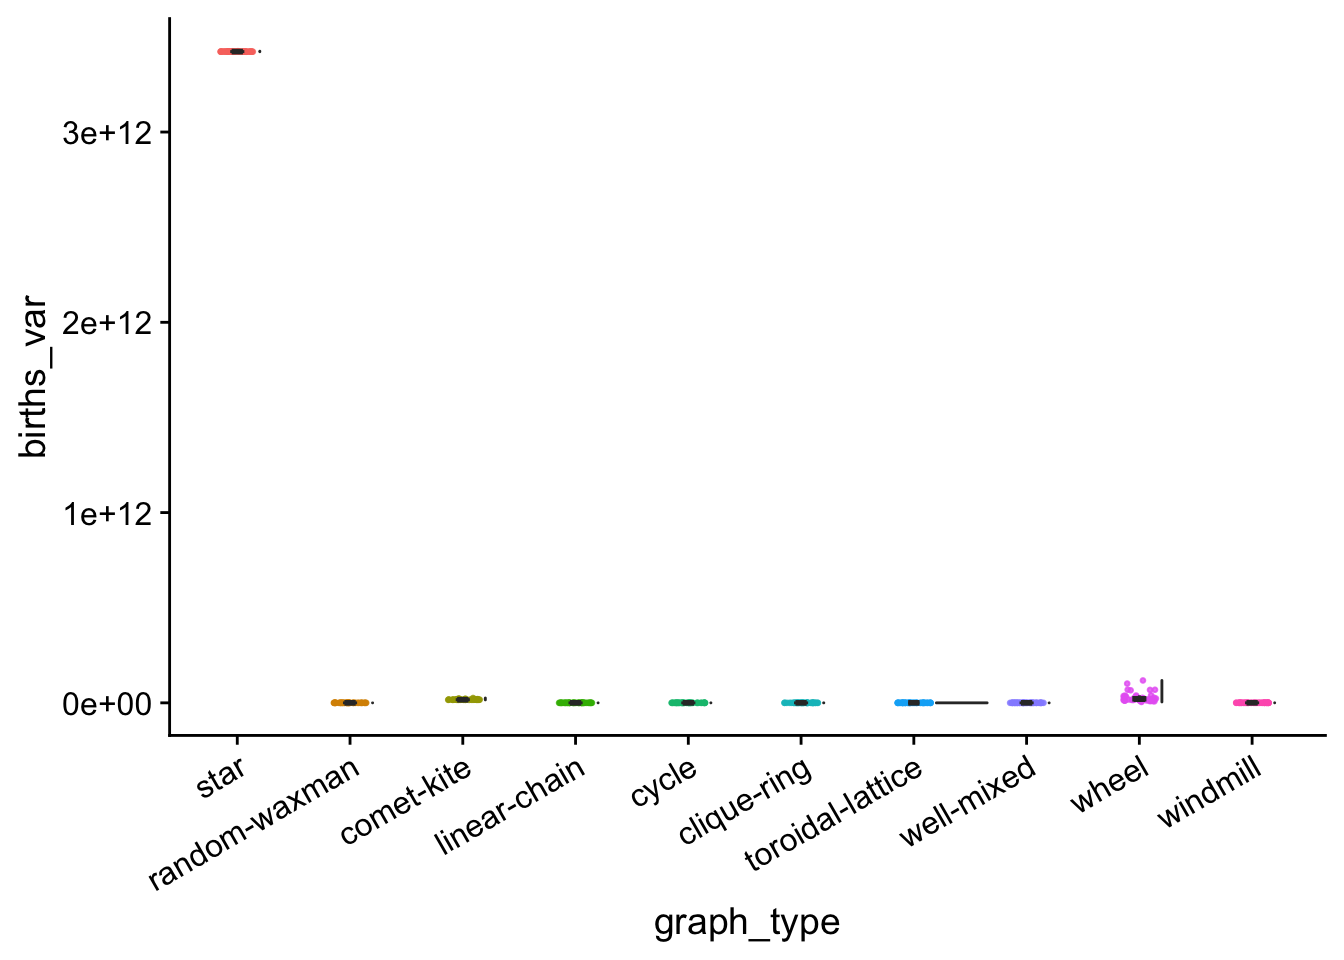
\includegraphics{supplemental-material_files/figure-latex/unnamed-chunk-73-1.pdf}

\hypertarget{task-appearances-total}{%
\subsection{Task appearances total}\label{task-appearances-total}}

\begin{Shaded}
\begin{Highlighting}[]
\NormalTok{task\_apps\_total\_plt }\OtherTok{\textless{}{-}} \FunctionTok{ggplot}\NormalTok{(}
    \AttributeTok{data =}\NormalTok{ graph\_loc\_data\_summary,}
    \AttributeTok{mapping =} \FunctionTok{aes}\NormalTok{(}
      \AttributeTok{x =}\NormalTok{ graph\_type,}
      \AttributeTok{y =}\NormalTok{ task\_apps\_total,}
      \AttributeTok{fill =}\NormalTok{ graph\_type}
\NormalTok{    )}
\NormalTok{  ) }\SpecialCharTok{+}
  \FunctionTok{geom\_flat\_violin}\NormalTok{(}
    \AttributeTok{position =} \FunctionTok{position\_nudge}\NormalTok{(}\AttributeTok{x =}\NormalTok{ .}\DecValTok{2}\NormalTok{, }\AttributeTok{y =} \DecValTok{0}\NormalTok{),}
    \AttributeTok{alpha =}\NormalTok{ .}\DecValTok{8}
\NormalTok{  ) }\SpecialCharTok{+}
  \FunctionTok{geom\_point}\NormalTok{(}
    \AttributeTok{mapping=}\FunctionTok{aes}\NormalTok{(}\AttributeTok{color =}\NormalTok{ graph\_type),}
    \AttributeTok{position =} \FunctionTok{position\_jitter}\NormalTok{(}\AttributeTok{width =}\NormalTok{ .}\DecValTok{15}\NormalTok{),}
    \AttributeTok{size =}\NormalTok{ .}\DecValTok{5}\NormalTok{,}
    \AttributeTok{alpha =} \FloatTok{0.8}
\NormalTok{  ) }\SpecialCharTok{+}
  \FunctionTok{geom\_boxplot}\NormalTok{(}
    \AttributeTok{width =}\NormalTok{ .}\DecValTok{1}\NormalTok{,}
    \AttributeTok{outlier.shape =} \ConstantTok{NA}\NormalTok{,}
    \AttributeTok{alpha =} \FloatTok{0.5}
\NormalTok{  ) }\SpecialCharTok{+}
  \FunctionTok{theme}\NormalTok{(}
    \AttributeTok{legend.position =} \StringTok{"none"}\NormalTok{,}
    \AttributeTok{axis.text.x =} \FunctionTok{element\_text}\NormalTok{(}
      \AttributeTok{angle =} \DecValTok{30}\NormalTok{,}
      \AttributeTok{hjust =} \DecValTok{1}
\NormalTok{    )}
\NormalTok{  )}

\FunctionTok{ggsave}\NormalTok{(}
  \AttributeTok{filename =} \FunctionTok{paste0}\NormalTok{(plot\_dir, }\StringTok{"/task\_apps\_total.pdf"}\NormalTok{),}
  \AttributeTok{plot =}\NormalTok{ task\_apps\_total\_plt,}
  \AttributeTok{width =} \DecValTok{15}\NormalTok{,}
  \AttributeTok{height =} \DecValTok{10}
\NormalTok{)}

\NormalTok{task\_apps\_total\_plt}
\end{Highlighting}
\end{Shaded}

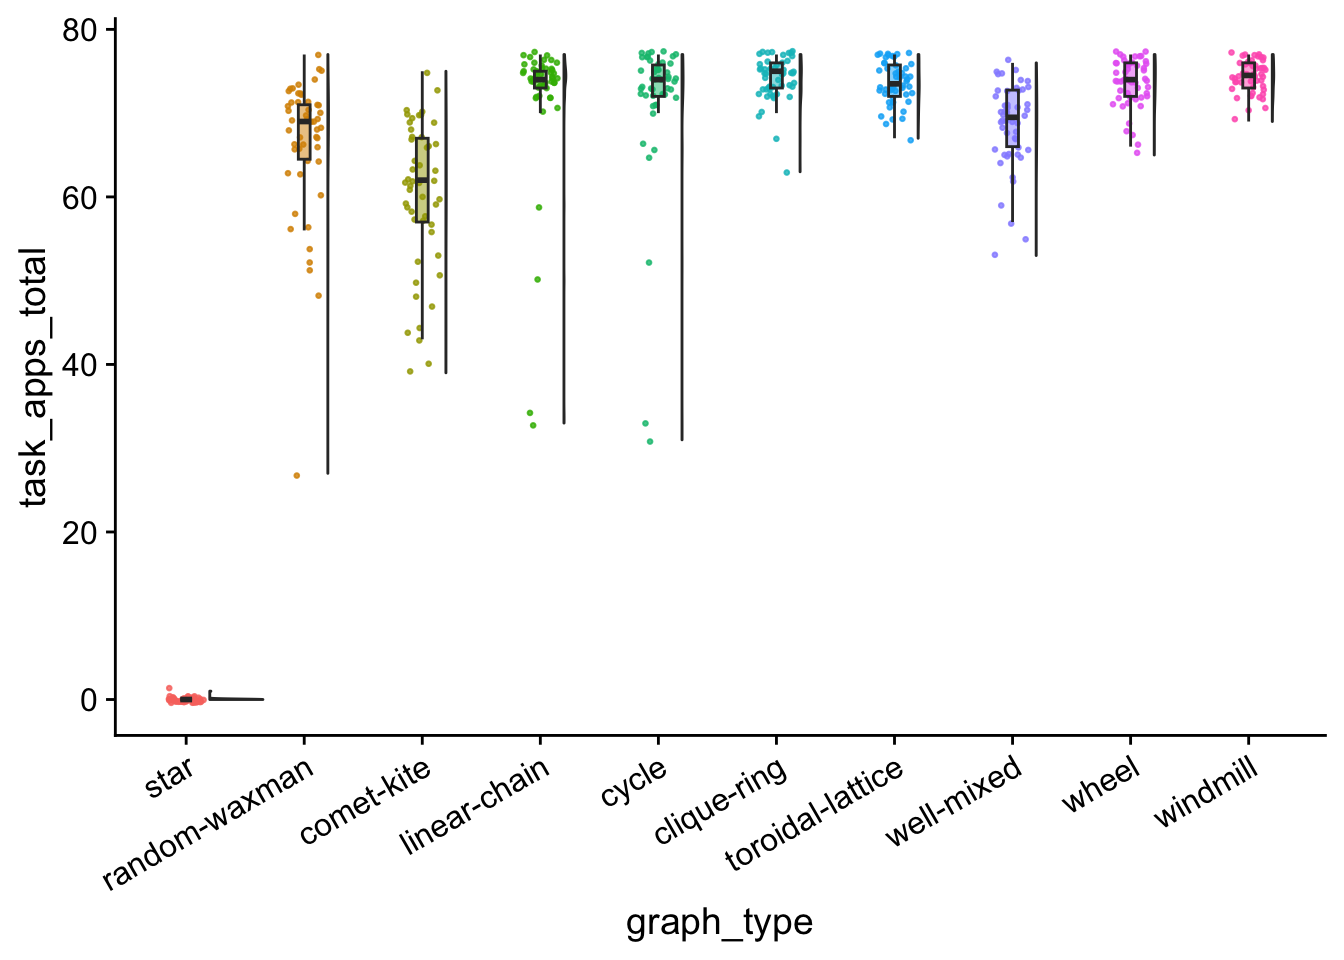
\includegraphics{supplemental-material_files/figure-latex/unnamed-chunk-74-1.pdf}

\begin{Shaded}
\begin{Highlighting}[]
\FunctionTok{kruskal.test}\NormalTok{(}
  \AttributeTok{formula =}\NormalTok{ task\_apps\_total }\SpecialCharTok{\textasciitilde{}}\NormalTok{ graph\_type,}
  \AttributeTok{data =}\NormalTok{ graph\_loc\_data\_summary}
\NormalTok{)}
\end{Highlighting}
\end{Shaded}

\begin{verbatim}
## 
##  Kruskal-Wallis rank sum test
## 
## data:  task_apps_total by graph_type
## Kruskal-Wallis chi-squared = 288.67, df = 9, p-value < 2.2e-16
\end{verbatim}

\begin{Shaded}
\begin{Highlighting}[]
\NormalTok{wc\_results }\OtherTok{\textless{}{-}} \FunctionTok{pairwise.wilcox.test}\NormalTok{(}
  \AttributeTok{x =}\NormalTok{ graph\_loc\_data\_summary}\SpecialCharTok{$}\NormalTok{task\_apps\_total,}
  \AttributeTok{g =}\NormalTok{ graph\_loc\_data\_summary}\SpecialCharTok{$}\NormalTok{graph\_type,}
  \AttributeTok{p.adjust.method   =} \StringTok{"holm"}\NormalTok{,}
  \AttributeTok{exact =} \ConstantTok{FALSE}

\NormalTok{)}
\NormalTok{wc\_results}
\end{Highlighting}
\end{Shaded}

\begin{verbatim}
## 
##  Pairwise comparisons using Wilcoxon rank sum test with continuity correction 
## 
## data:  graph_loc_data_summary$task_apps_total and graph_loc_data_summary$graph_type 
## 
##                  star    random-waxman comet-kite linear-chain cycle  
## random-waxman    < 2e-16 -             -          -            -      
## comet-kite       < 2e-16 0.00089       -          -            -      
## linear-chain     < 2e-16 2.8e-08       2.7e-11    -            -      
## cycle            < 2e-16 8.3e-07       6.3e-11    1.00000      -      
## clique-ring      < 2e-16 4.4e-10       2.0e-14    1.00000      1.00000
## toroidal-lattice < 2e-16 1.2e-08       3.7e-14    1.00000      1.00000
## well-mixed       < 2e-16 1.00000       3.5e-06    8.8e-07      2.1e-05
## wheel            < 2e-16 1.4e-08       8.1e-14    1.00000      1.00000
## windmill         < 2e-16 2.7e-11       4.3e-15    1.00000      1.00000
##                  clique-ring toroidal-lattice well-mixed wheel  
## random-waxman    -           -                -          -      
## comet-kite       -           -                -          -      
## linear-chain     -           -                -          -      
## cycle            -           -                -          -      
## clique-ring      -           -                -          -      
## toroidal-lattice 1.00000     -                -          -      
## well-mixed       2.3e-08     7.7e-07          -          -      
## wheel            1.00000     1.00000          5.0e-07    -      
## windmill         1.00000     1.00000          1.2e-09    1.00000
## 
## P value adjustment method: holm
\end{verbatim}

\hypertarget{avida---squished-lattice-experiment-analyses}{%
\chapter{Avida - Squished lattice experiment analyses}\label{avida---squished-lattice-experiment-analyses}}

\hypertarget{dependencies-and-setup-2}{%
\section{Dependencies and setup}\label{dependencies-and-setup-2}}

\begin{Shaded}
\begin{Highlighting}[]
\FunctionTok{library}\NormalTok{(tidyverse)}
\FunctionTok{library}\NormalTok{(cowplot)}
\FunctionTok{library}\NormalTok{(RColorBrewer)}
\FunctionTok{library}\NormalTok{(khroma)}
\FunctionTok{library}\NormalTok{(rstatix)}
\FunctionTok{library}\NormalTok{(knitr)}
\FunctionTok{library}\NormalTok{(kableExtra)}
\FunctionTok{source}\NormalTok{(}\StringTok{"https://gist.githubusercontent.com/benmarwick/2a1bb0133ff568cbe28d/raw/fb53bd97121f7f9ce947837ef1a4c65a73bffb3f/geom\_flat\_violin.R"}\NormalTok{)}
\end{Highlighting}
\end{Shaded}

\begin{Shaded}
\begin{Highlighting}[]
\CommentTok{\# Check if Rmd is being compiled using bookdown}
\NormalTok{bookdown }\OtherTok{\textless{}{-}} \FunctionTok{exists}\NormalTok{(}\StringTok{"bookdown\_build"}\NormalTok{)}
\end{Highlighting}
\end{Shaded}

\begin{Shaded}
\begin{Highlighting}[]
\NormalTok{experiment\_slug }\OtherTok{\textless{}{-}} \StringTok{"2025{-}04{-}17{-}squished{-}lattice{-}longer"}
\NormalTok{working\_directory }\OtherTok{\textless{}{-}} \FunctionTok{paste}\NormalTok{(}
  \StringTok{"experiments"}\NormalTok{,}
\NormalTok{  experiment\_slug,}
  \StringTok{"analysis"}\NormalTok{,}
  \AttributeTok{sep =} \StringTok{"/"}
\NormalTok{)}
\CommentTok{\# Adjust working directory if being knitted for bookdown build.}
\ControlFlowTok{if}\NormalTok{ (bookdown) \{}
\NormalTok{  working\_directory }\OtherTok{\textless{}{-}} \FunctionTok{paste0}\NormalTok{(}
\NormalTok{    bookdown\_wd\_prefix,}
\NormalTok{    working\_directory}
\NormalTok{  )}
\NormalTok{\}}
\end{Highlighting}
\end{Shaded}

\begin{Shaded}
\begin{Highlighting}[]
\CommentTok{\# Configure our default graphing theme}
\FunctionTok{theme\_set}\NormalTok{(}\FunctionTok{theme\_cowplot}\NormalTok{())}
\CommentTok{\# Create a directory to store plots}
\NormalTok{plot\_dir }\OtherTok{\textless{}{-}} \FunctionTok{paste}\NormalTok{(}
\NormalTok{  working\_directory,}
  \StringTok{"plots"}\NormalTok{,}
  \AttributeTok{sep =} \StringTok{"/"}
\NormalTok{)}

\FunctionTok{dir.create}\NormalTok{(}
\NormalTok{  plot\_dir,}
  \AttributeTok{showWarnings =} \ConstantTok{FALSE}
\NormalTok{)}
\end{Highlighting}
\end{Shaded}

\begin{Shaded}
\begin{Highlighting}[]
\NormalTok{focal\_graphs }\OtherTok{\textless{}{-}} \FunctionTok{c}\NormalTok{(}
  \StringTok{"toroidal{-}lattice\_60x60"}\NormalTok{,}
  \StringTok{"toroidal{-}lattice\_15x240"}\NormalTok{,}
  \StringTok{"toroidal{-}lattice\_2x1800"}\NormalTok{,}
  \StringTok{"cycle"}
\NormalTok{)}

\CommentTok{\# Load summary data from final update}
\NormalTok{data\_path }\OtherTok{\textless{}{-}} \FunctionTok{paste}\NormalTok{(}
\NormalTok{  working\_directory,}
  \StringTok{"data"}\NormalTok{,}
  \StringTok{"summary.csv"}\NormalTok{,}
  \AttributeTok{sep =} \StringTok{"/"}
\NormalTok{)}
\NormalTok{data }\OtherTok{\textless{}{-}} \FunctionTok{read\_csv}\NormalTok{(data\_path)}

\NormalTok{data }\OtherTok{\textless{}{-}}\NormalTok{ data }\SpecialCharTok{\%\textgreater{}\%}
  \FunctionTok{filter}\NormalTok{(graph\_type }\SpecialCharTok{\%in\%}\NormalTok{ focal\_graphs) }\SpecialCharTok{\%\textgreater{}\%}
  \FunctionTok{mutate}\NormalTok{(}
    \AttributeTok{graph\_type =} \FunctionTok{factor}\NormalTok{(}
\NormalTok{      graph\_type,}
      \AttributeTok{levels =}\NormalTok{ focal\_graphs}
\NormalTok{    ),}
    \AttributeTok{ENVIRONMENT\_FILE =} \FunctionTok{as.factor}\NormalTok{(ENVIRONMENT\_FILE)}
\NormalTok{  )}
\end{Highlighting}
\end{Shaded}

\begin{Shaded}
\begin{Highlighting}[]
\NormalTok{time\_series\_path }\OtherTok{\textless{}{-}} \FunctionTok{paste}\NormalTok{(}
\NormalTok{  working\_directory,}
  \StringTok{"data"}\NormalTok{,}
  \StringTok{"time\_series.csv"}\NormalTok{,}
  \AttributeTok{sep =} \StringTok{"/"}
\NormalTok{)}
\NormalTok{time\_series\_data }\OtherTok{\textless{}{-}} \FunctionTok{read\_csv}\NormalTok{(time\_series\_path)}

\NormalTok{time\_series\_data }\OtherTok{\textless{}{-}}\NormalTok{ time\_series\_data }\SpecialCharTok{\%\textgreater{}\%}
  \FunctionTok{filter}\NormalTok{(graph\_type }\SpecialCharTok{\%in\%}\NormalTok{ focal\_graphs) }\SpecialCharTok{\%\textgreater{}\%}
  \FunctionTok{mutate}\NormalTok{(}
    \AttributeTok{graph\_type =} \FunctionTok{factor}\NormalTok{(}
\NormalTok{      graph\_type,}
      \AttributeTok{levels =}\NormalTok{ focal\_graphs}
\NormalTok{    ),}
    \AttributeTok{ENVIRONMENT\_FILE =} \FunctionTok{as.factor}\NormalTok{(ENVIRONMENT\_FILE),}
    \AttributeTok{seed =} \FunctionTok{as.factor}\NormalTok{(seed)}
\NormalTok{  )}
\NormalTok{time\_series\_data }\OtherTok{\textless{}{-}}\NormalTok{ time\_series\_data }\SpecialCharTok{\%\textgreater{}\%} \FunctionTok{filter}\NormalTok{(seed }\SpecialCharTok{\%in\%}\NormalTok{ data}\SpecialCharTok{$}\NormalTok{seed)}
\end{Highlighting}
\end{Shaded}

\begin{Shaded}
\begin{Highlighting}[]
\CommentTok{\# Check that all runs completed}
\NormalTok{data }\SpecialCharTok{\%\textgreater{}\%}
  \FunctionTok{filter}\NormalTok{(update }\SpecialCharTok{==} \DecValTok{400000}\NormalTok{) }\SpecialCharTok{\%\textgreater{}\%}
  \FunctionTok{group\_by}\NormalTok{(graph\_type) }\SpecialCharTok{\%\textgreater{}\%}
  \FunctionTok{summarize}\NormalTok{(}
    \AttributeTok{n =} \FunctionTok{n}\NormalTok{()}
\NormalTok{  )}
\end{Highlighting}
\end{Shaded}

\begin{verbatim}
## # A tibble: 4 x 2
##   graph_type                  n
##   <fct>                   <int>
## 1 toroidal-lattice_60x60     50
## 2 toroidal-lattice_15x240    50
## 3 toroidal-lattice_2x1800    50
## 4 cycle                      50
\end{verbatim}

\hypertarget{number-of-tasks-completed-1}{%
\section{Number of tasks completed}\label{number-of-tasks-completed-1}}

\begin{Shaded}
\begin{Highlighting}[]
\NormalTok{pop\_tasks\_total\_plt }\OtherTok{\textless{}{-}} \FunctionTok{ggplot}\NormalTok{(}
  \AttributeTok{data =}\NormalTok{ data,}
  \AttributeTok{mapping =} \FunctionTok{aes}\NormalTok{(}
    \AttributeTok{x =}\NormalTok{ graph\_type,}
    \AttributeTok{y =}\NormalTok{ pop\_task\_total,}
    \AttributeTok{fill =}\NormalTok{ graph\_type}
\NormalTok{  )}
\NormalTok{) }\SpecialCharTok{+}
  \FunctionTok{geom\_flat\_violin}\NormalTok{(}
    \AttributeTok{position =} \FunctionTok{position\_nudge}\NormalTok{(}\AttributeTok{x =}\NormalTok{ .}\DecValTok{2}\NormalTok{, }\AttributeTok{y =} \DecValTok{0}\NormalTok{),}
    \AttributeTok{alpha =}\NormalTok{ .}\DecValTok{8}
\NormalTok{  ) }\SpecialCharTok{+}
  \FunctionTok{geom\_point}\NormalTok{(}
    \AttributeTok{mapping=}\FunctionTok{aes}\NormalTok{(}\AttributeTok{color =}\NormalTok{ graph\_type),}
    \AttributeTok{position =} \FunctionTok{position\_jitter}\NormalTok{(}\AttributeTok{width =}\NormalTok{ .}\DecValTok{15}\NormalTok{),}
    \AttributeTok{size =}\NormalTok{ .}\DecValTok{5}\NormalTok{,}
    \AttributeTok{alpha =} \FloatTok{0.8}
\NormalTok{  ) }\SpecialCharTok{+}
  \FunctionTok{geom\_boxplot}\NormalTok{(}
    \AttributeTok{width =}\NormalTok{ .}\DecValTok{1}\NormalTok{,}
    \AttributeTok{outlier.shape =} \ConstantTok{NA}\NormalTok{,}
    \AttributeTok{alpha =} \FloatTok{0.5}
\NormalTok{  ) }\SpecialCharTok{+}
  \FunctionTok{theme}\NormalTok{(}
    \AttributeTok{legend.position =} \StringTok{"none"}\NormalTok{,}
    \AttributeTok{axis.text.x =} \FunctionTok{element\_text}\NormalTok{(}
      \AttributeTok{angle =} \DecValTok{30}\NormalTok{,}
      \AttributeTok{hjust =} \DecValTok{1}
\NormalTok{    )}
\NormalTok{  )}

\FunctionTok{ggsave}\NormalTok{(}
  \AttributeTok{filename =} \FunctionTok{paste0}\NormalTok{(plot\_dir, }\StringTok{"/pop\_tasks\_total.pdf"}\NormalTok{),}
  \AttributeTok{plot =}\NormalTok{ pop\_tasks\_total\_plt,}
  \AttributeTok{width =} \DecValTok{15}\NormalTok{,}
  \AttributeTok{height =} \DecValTok{10}
\NormalTok{)}

\NormalTok{pop\_tasks\_total\_plt}
\end{Highlighting}
\end{Shaded}

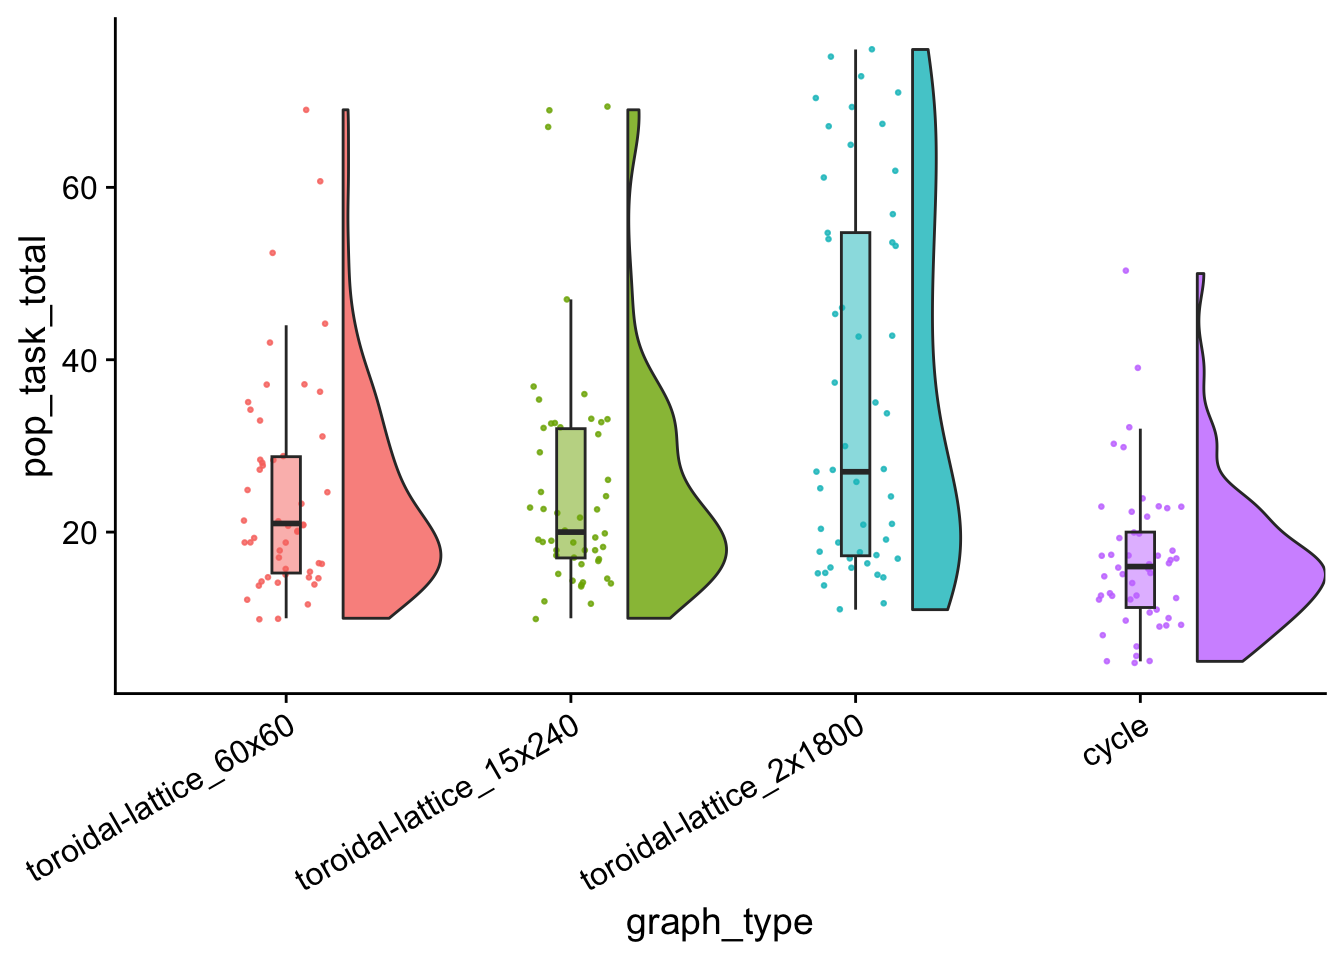
\includegraphics{supplemental-material_files/figure-latex/unnamed-chunk-83-1.pdf}

\begin{Shaded}
\begin{Highlighting}[]
\NormalTok{data }\SpecialCharTok{\%\textgreater{}\%}
  \FunctionTok{group\_by}\NormalTok{(graph\_type) }\SpecialCharTok{\%\textgreater{}\%}
  \FunctionTok{summarize}\NormalTok{(}
    \AttributeTok{reps =} \FunctionTok{n}\NormalTok{(),}
    \AttributeTok{median\_pop\_tasks =} \FunctionTok{median}\NormalTok{(pop\_task\_total),}
    \AttributeTok{mean\_pop\_tasks =} \FunctionTok{mean}\NormalTok{(pop\_task\_total)}
\NormalTok{  ) }\SpecialCharTok{\%\textgreater{}\%}
  \FunctionTok{arrange}\NormalTok{(}
    \FunctionTok{desc}\NormalTok{(mean\_pop\_tasks)}
\NormalTok{  )}
\end{Highlighting}
\end{Shaded}

\begin{verbatim}
## # A tibble: 4 x 4
##   graph_type               reps median_pop_tasks mean_pop_tasks
##   <fct>                   <int>            <dbl>          <dbl>
## 1 toroidal-lattice_2x1800    50               27           36.6
## 2 toroidal-lattice_15x240    50               20           25.2
## 3 toroidal-lattice_60x60     50               21           24.6
## 4 cycle                      50               16           16.7
\end{verbatim}

\begin{Shaded}
\begin{Highlighting}[]
\FunctionTok{kruskal.test}\NormalTok{(}
  \AttributeTok{formula =}\NormalTok{ pop\_task\_total }\SpecialCharTok{\textasciitilde{}}\NormalTok{ graph\_type,}
  \AttributeTok{data =}\NormalTok{ data}
\NormalTok{)}
\end{Highlighting}
\end{Shaded}

\begin{verbatim}
## 
##  Kruskal-Wallis rank sum test
## 
## data:  pop_task_total by graph_type
## Kruskal-Wallis chi-squared = 34.696, df = 3, p-value = 1.412e-07
\end{verbatim}

\begin{Shaded}
\begin{Highlighting}[]
\NormalTok{wc\_results }\OtherTok{\textless{}{-}} \FunctionTok{pairwise.wilcox.test}\NormalTok{(}
  \AttributeTok{x =}\NormalTok{ data}\SpecialCharTok{$}\NormalTok{pop\_task\_total,}
  \AttributeTok{g =}\NormalTok{ data}\SpecialCharTok{$}\NormalTok{graph\_type,}
  \AttributeTok{p.adjust.method   =} \StringTok{"holm"}\NormalTok{,}
  \AttributeTok{exact =} \ConstantTok{FALSE}

\NormalTok{)}

\NormalTok{pop\_task\_wc\_table }\OtherTok{\textless{}{-}} \FunctionTok{kbl}\NormalTok{(wc\_results}\SpecialCharTok{$}\NormalTok{p.value) }\SpecialCharTok{\%\textgreater{}\%} \FunctionTok{kable\_styling}\NormalTok{()}
\FunctionTok{save\_kable}\NormalTok{(pop\_task\_wc\_table, }\FunctionTok{paste0}\NormalTok{(plot\_dir, }\StringTok{"/pop\_task\_wc\_table.pdf"}\NormalTok{))}

\NormalTok{pop\_task\_wc\_table}
\end{Highlighting}
\end{Shaded}

\begin{table}
\centering
\begin{tabular}[t]{l|r|r|r}
\hline
  & toroidal-lattice\_60x60 & toroidal-lattice\_15x240 & toroidal-lattice\_2x1800\\
\hline
toroidal-lattice\_15x240 & 0.9011082 & NA & NA\\
\hline
toroidal-lattice\_2x1800 & 0.0313929 & 0.0386732 & NA\\
\hline
cycle & 0.0010892 & 0.0002773 & 8e-07\\
\hline
\end{tabular}
\end{table}

\hypertarget{dominant-tasks-1}{%
\section{Dominant tasks}\label{dominant-tasks-1}}

\begin{Shaded}
\begin{Highlighting}[]
\NormalTok{dom\_tasks\_total\_plt }\OtherTok{\textless{}{-}} \FunctionTok{ggplot}\NormalTok{(}
  \AttributeTok{data =}\NormalTok{ data,}
  \AttributeTok{mapping =} \FunctionTok{aes}\NormalTok{(}
    \AttributeTok{x =}\NormalTok{ graph\_type,}
    \AttributeTok{y =}\NormalTok{ dom\_task\_total,}
    \AttributeTok{fill =}\NormalTok{ graph\_type}
\NormalTok{  )}
\NormalTok{) }\SpecialCharTok{+}
  \FunctionTok{geom\_flat\_violin}\NormalTok{(}
    \AttributeTok{position =} \FunctionTok{position\_nudge}\NormalTok{(}\AttributeTok{x =}\NormalTok{ .}\DecValTok{2}\NormalTok{, }\AttributeTok{y =} \DecValTok{0}\NormalTok{),}
    \AttributeTok{alpha =}\NormalTok{ .}\DecValTok{8}
\NormalTok{  ) }\SpecialCharTok{+}
  \FunctionTok{geom\_point}\NormalTok{(}
    \AttributeTok{mapping=}\FunctionTok{aes}\NormalTok{(}\AttributeTok{color =}\NormalTok{ graph\_type),}
    \AttributeTok{position =} \FunctionTok{position\_jitter}\NormalTok{(}\AttributeTok{width =}\NormalTok{ .}\DecValTok{15}\NormalTok{),}
    \AttributeTok{size =}\NormalTok{ .}\DecValTok{5}\NormalTok{,}
    \AttributeTok{alpha =} \FloatTok{0.8}
\NormalTok{  ) }\SpecialCharTok{+}
  \FunctionTok{geom\_boxplot}\NormalTok{(}
    \AttributeTok{width =}\NormalTok{ .}\DecValTok{1}\NormalTok{,}
    \AttributeTok{outlier.shape =} \ConstantTok{NA}\NormalTok{,}
    \AttributeTok{alpha =} \FloatTok{0.5}
\NormalTok{  ) }\SpecialCharTok{+}
  \FunctionTok{theme}\NormalTok{(}
    \AttributeTok{legend.position =} \StringTok{"none"}\NormalTok{,}
    \AttributeTok{axis.text.x =} \FunctionTok{element\_text}\NormalTok{(}
      \AttributeTok{angle =} \DecValTok{30}\NormalTok{,}
      \AttributeTok{hjust =} \DecValTok{1}
\NormalTok{    )}
\NormalTok{  )}

\FunctionTok{ggsave}\NormalTok{(}
  \AttributeTok{filename =} \FunctionTok{paste0}\NormalTok{(plot\_dir, }\StringTok{"/dom\_tasks\_total.pdf"}\NormalTok{),}
  \AttributeTok{plot =}\NormalTok{ dom\_tasks\_total\_plt,}
  \AttributeTok{width =} \DecValTok{15}\NormalTok{,}
  \AttributeTok{height =} \DecValTok{10}
\NormalTok{)}

\NormalTok{dom\_tasks\_total\_plt}
\end{Highlighting}
\end{Shaded}

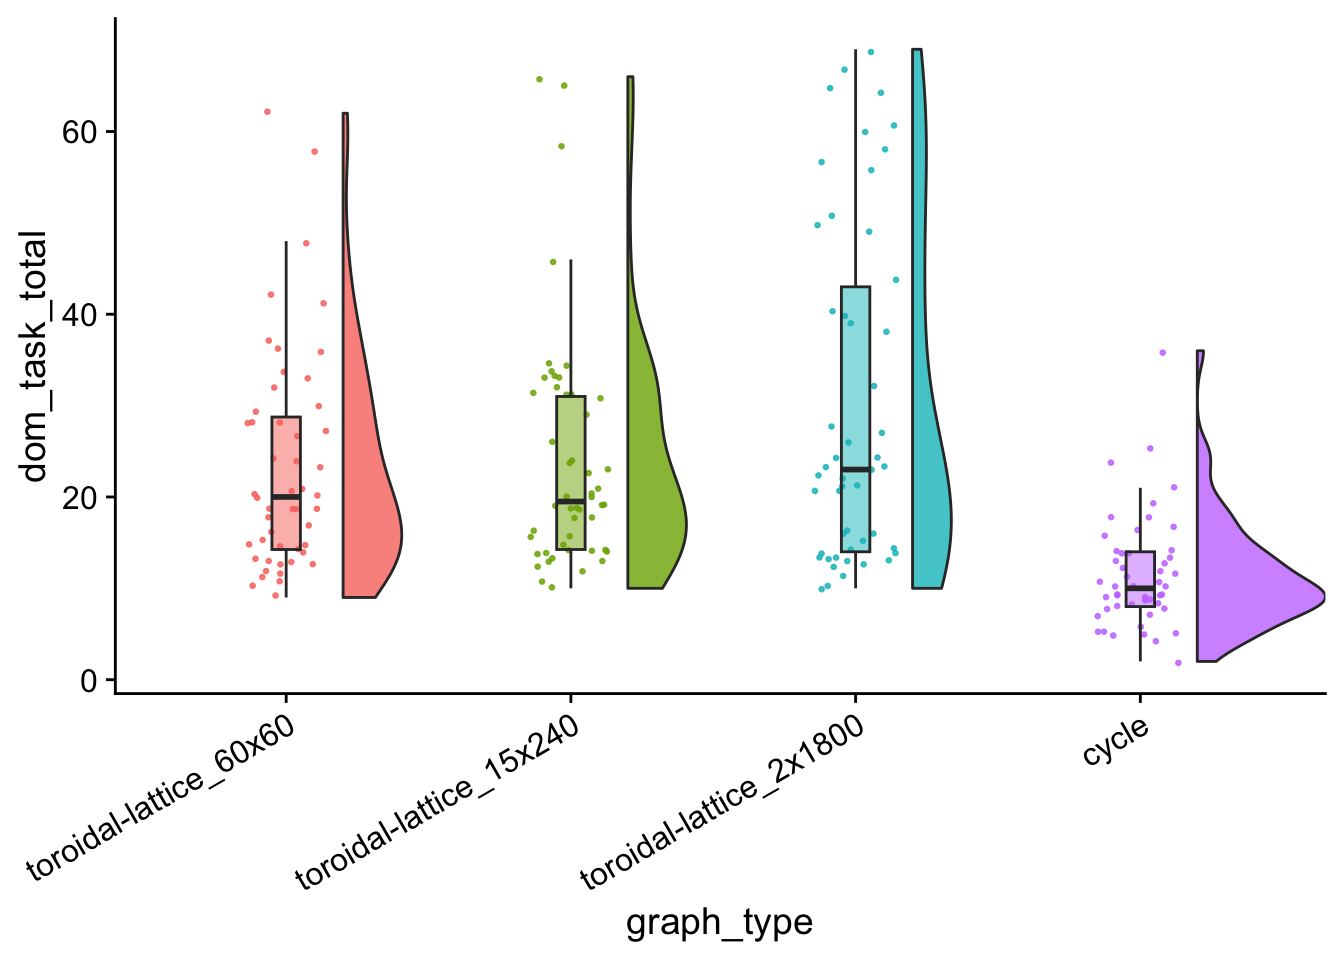
\includegraphics{supplemental-material_files/figure-latex/unnamed-chunk-86-1.pdf}

\begin{Shaded}
\begin{Highlighting}[]
\NormalTok{data }\SpecialCharTok{\%\textgreater{}\%}
  \FunctionTok{group\_by}\NormalTok{(graph\_type) }\SpecialCharTok{\%\textgreater{}\%}
  \FunctionTok{summarize}\NormalTok{(}
    \AttributeTok{reps =} \FunctionTok{n}\NormalTok{(),}
    \AttributeTok{median\_dom\_task\_total =} \FunctionTok{median}\NormalTok{(dom\_task\_total),}
    \AttributeTok{mean\_dom\_task\_total =} \FunctionTok{mean}\NormalTok{(dom\_task\_total)}
\NormalTok{  ) }\SpecialCharTok{\%\textgreater{}\%}
  \FunctionTok{arrange}\NormalTok{(}
    \FunctionTok{desc}\NormalTok{(mean\_dom\_task\_total)}
\NormalTok{  )}
\end{Highlighting}
\end{Shaded}

\begin{verbatim}
## # A tibble: 4 x 4
##   graph_type               reps median_dom_task_total mean_dom_task_total
##   <fct>                   <int>                 <dbl>               <dbl>
## 1 toroidal-lattice_2x1800    50                  23                  30.1
## 2 toroidal-lattice_15x240    50                  19.5                24.1
## 3 toroidal-lattice_60x60     50                  20                  23.5
## 4 cycle                      50                  10                  11.5
\end{verbatim}

\begin{Shaded}
\begin{Highlighting}[]
\FunctionTok{kruskal.test}\NormalTok{(}
  \AttributeTok{formula =}\NormalTok{ dom\_task\_total }\SpecialCharTok{\textasciitilde{}}\NormalTok{ graph\_type,}
  \AttributeTok{data =}\NormalTok{ data}
\NormalTok{)}
\end{Highlighting}
\end{Shaded}

\begin{verbatim}
## 
##  Kruskal-Wallis rank sum test
## 
## data:  dom_task_total by graph_type
## Kruskal-Wallis chi-squared = 62.705, df = 3, p-value = 1.553e-13
\end{verbatim}

\begin{Shaded}
\begin{Highlighting}[]
\NormalTok{wc\_results }\OtherTok{\textless{}{-}} \FunctionTok{pairwise.wilcox.test}\NormalTok{(}
  \AttributeTok{x =}\NormalTok{ data}\SpecialCharTok{$}\NormalTok{dom\_task\_total,}
  \AttributeTok{g =}\NormalTok{ data}\SpecialCharTok{$}\NormalTok{graph\_type,}
  \AttributeTok{p.adjust.method   =} \StringTok{"holm"}\NormalTok{,}
  \AttributeTok{exact =} \ConstantTok{FALSE}
\NormalTok{)}

\NormalTok{dom\_task\_total\_wc\_table }\OtherTok{\textless{}{-}} \FunctionTok{kbl}\NormalTok{(wc\_results}\SpecialCharTok{$}\NormalTok{p.value) }\SpecialCharTok{\%\textgreater{}\%} \FunctionTok{kable\_styling}\NormalTok{()}
\FunctionTok{save\_kable}\NormalTok{(dom\_task\_total\_wc\_table, }\FunctionTok{paste0}\NormalTok{(plot\_dir, }\StringTok{"/dom\_task\_total\_wc\_table.pdf"}\NormalTok{))}

\NormalTok{dom\_task\_total\_wc\_table}
\end{Highlighting}
\end{Shaded}

\begin{table}
\centering
\begin{tabular}[t]{l|r|r|r}
\hline
  & toroidal-lattice\_60x60 & toroidal-lattice\_15x240 & toroidal-lattice\_2x1800\\
\hline
toroidal-lattice\_15x240 & 0.8224738 & NA & NA\\
\hline
toroidal-lattice\_2x1800 & 0.4960864 & 0.5387756 & NA\\
\hline
cycle & 0.0000000 & 0.0000000 & 0\\
\hline
\end{tabular}
\end{table}

Tasks done by organisms not in dominant taxon:

\begin{Shaded}
\begin{Highlighting}[]
\NormalTok{data }\OtherTok{\textless{}{-}}\NormalTok{ data }\SpecialCharTok{\%\textgreater{}\%}
  \FunctionTok{mutate}\NormalTok{(}
    \AttributeTok{nondom\_pop\_task\_prop =} \FunctionTok{case\_when}\NormalTok{(}
\NormalTok{      pop\_task\_total }\SpecialCharTok{==} \DecValTok{0} \SpecialCharTok{\textasciitilde{}} \DecValTok{0}\NormalTok{,}
      \AttributeTok{.default =}\NormalTok{ (pop\_task\_total }\SpecialCharTok{{-}}\NormalTok{ dom\_task\_total) }\SpecialCharTok{/}\NormalTok{ (pop\_task\_total)}
\NormalTok{    )}
\NormalTok{  )}
\NormalTok{nondom\_tasks\_total\_plt }\OtherTok{\textless{}{-}} \FunctionTok{ggplot}\NormalTok{(}
    \AttributeTok{data =}\NormalTok{ data,}
    \AttributeTok{mapping =} \FunctionTok{aes}\NormalTok{(}
      \AttributeTok{x =}\NormalTok{ graph\_type,}
      \AttributeTok{y =}\NormalTok{ nondom\_pop\_task\_prop,}
      \AttributeTok{fill =}\NormalTok{ graph\_type}
\NormalTok{    )}
\NormalTok{  ) }\SpecialCharTok{+}
  \FunctionTok{geom\_flat\_violin}\NormalTok{(}
    \AttributeTok{position =} \FunctionTok{position\_nudge}\NormalTok{(}\AttributeTok{x =}\NormalTok{ .}\DecValTok{2}\NormalTok{, }\AttributeTok{y =} \DecValTok{0}\NormalTok{),}
    \AttributeTok{alpha =}\NormalTok{ .}\DecValTok{8}
\NormalTok{  ) }\SpecialCharTok{+}
  \FunctionTok{geom\_point}\NormalTok{(}
    \AttributeTok{mapping=}\FunctionTok{aes}\NormalTok{(}\AttributeTok{color =}\NormalTok{ graph\_type),}
    \AttributeTok{position =} \FunctionTok{position\_jitter}\NormalTok{(}\AttributeTok{width =}\NormalTok{ .}\DecValTok{15}\NormalTok{),}
    \AttributeTok{size =}\NormalTok{ .}\DecValTok{5}\NormalTok{,}
    \AttributeTok{alpha =} \FloatTok{0.8}
\NormalTok{  ) }\SpecialCharTok{+}
  \FunctionTok{geom\_boxplot}\NormalTok{(}
    \AttributeTok{width =}\NormalTok{ .}\DecValTok{1}\NormalTok{,}
    \AttributeTok{outlier.shape =} \ConstantTok{NA}\NormalTok{,}
    \AttributeTok{alpha =} \FloatTok{0.5}
\NormalTok{  ) }\SpecialCharTok{+}
  \FunctionTok{theme}\NormalTok{(}
    \AttributeTok{legend.position =} \StringTok{"none"}\NormalTok{,}
    \AttributeTok{axis.text.x =} \FunctionTok{element\_text}\NormalTok{(}
      \AttributeTok{angle =} \DecValTok{30}\NormalTok{,}
      \AttributeTok{hjust =} \DecValTok{1}
\NormalTok{    )}
\NormalTok{  )}

\FunctionTok{ggsave}\NormalTok{(}
  \AttributeTok{filename =} \FunctionTok{paste0}\NormalTok{(plot\_dir, }\StringTok{"/non\_dom\_tasks\_total.pdf"}\NormalTok{),}
  \AttributeTok{plot =}\NormalTok{ nondom\_tasks\_total\_plt,}
  \AttributeTok{width =} \DecValTok{15}\NormalTok{,}
  \AttributeTok{height =} \DecValTok{10}
\NormalTok{)}

\NormalTok{nondom\_tasks\_total\_plt}
\end{Highlighting}
\end{Shaded}

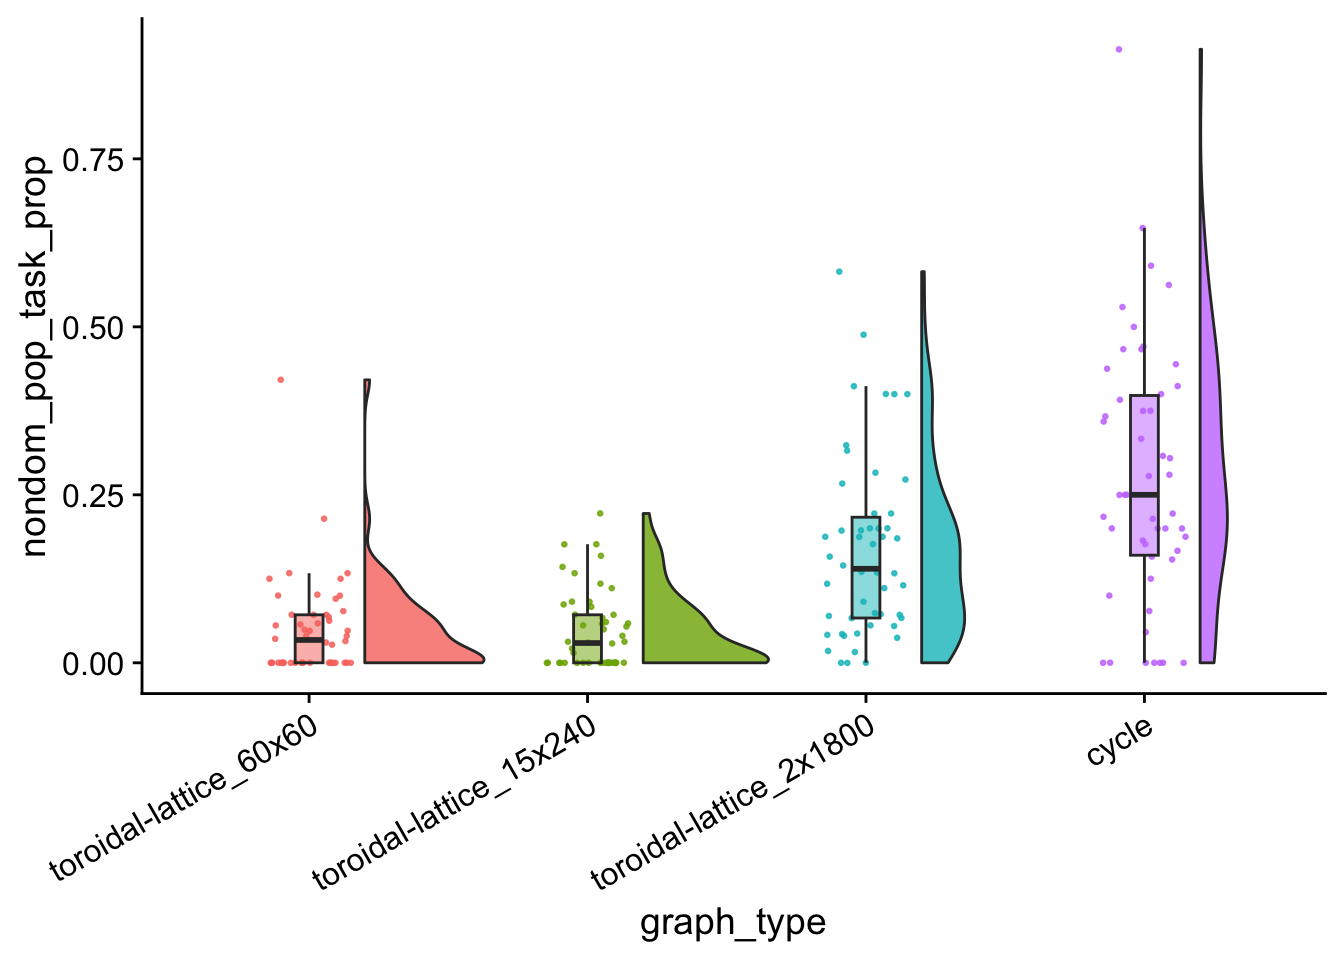
\includegraphics{supplemental-material_files/figure-latex/unnamed-chunk-89-1.pdf}

\begin{Shaded}
\begin{Highlighting}[]
\NormalTok{data }\SpecialCharTok{\%\textgreater{}\%}
  \FunctionTok{group\_by}\NormalTok{(graph\_type) }\SpecialCharTok{\%\textgreater{}\%}
  \FunctionTok{summarize}\NormalTok{(}
    \AttributeTok{reps =} \FunctionTok{n}\NormalTok{(),}
    \AttributeTok{median\_nondom\_pop\_task\_prop =} \FunctionTok{median}\NormalTok{(nondom\_pop\_task\_prop),}
    \AttributeTok{mean\_nondom\_pop\_task\_prop =} \FunctionTok{mean}\NormalTok{(nondom\_pop\_task\_prop)}
\NormalTok{  ) }\SpecialCharTok{\%\textgreater{}\%}
  \FunctionTok{arrange}\NormalTok{(}
    \FunctionTok{desc}\NormalTok{(mean\_nondom\_pop\_task\_prop)}
\NormalTok{  )}
\end{Highlighting}
\end{Shaded}

\begin{verbatim}
## # A tibble: 4 x 4
##   graph_type               reps median_nondom_pop_task_~1 mean_nondom_pop_task~2
##   <fct>                   <int>                     <dbl>                  <dbl>
## 1 cycle                      50                    0.25                   0.276 
## 2 toroidal-lattice_2x1800    50                    0.140                  0.168 
## 3 toroidal-lattice_60x60     50                    0.0340                 0.0498
## 4 toroidal-lattice_15x240    50                    0.0294                 0.0467
## # i abbreviated names: 1: median_nondom_pop_task_prop,
## #   2: mean_nondom_pop_task_prop
\end{verbatim}

\begin{Shaded}
\begin{Highlighting}[]
\FunctionTok{kruskal.test}\NormalTok{(}
  \AttributeTok{formula =}\NormalTok{ nondom\_pop\_task\_prop }\SpecialCharTok{\textasciitilde{}}\NormalTok{ graph\_type,}
  \AttributeTok{data =}\NormalTok{ data}
\NormalTok{)}
\end{Highlighting}
\end{Shaded}

\begin{verbatim}
## 
##  Kruskal-Wallis rank sum test
## 
## data:  nondom_pop_task_prop by graph_type
## Kruskal-Wallis chi-squared = 72.727, df = 3, p-value = 1.112e-15
\end{verbatim}

\begin{Shaded}
\begin{Highlighting}[]
\NormalTok{wc\_results }\OtherTok{\textless{}{-}} \FunctionTok{pairwise.wilcox.test}\NormalTok{(}
  \AttributeTok{x =}\NormalTok{ data}\SpecialCharTok{$}\NormalTok{nondom\_pop\_task\_prop,}
  \AttributeTok{g =}\NormalTok{ data}\SpecialCharTok{$}\NormalTok{graph\_type,}
  \AttributeTok{p.adjust.method   =} \StringTok{"holm"}\NormalTok{,}
  \AttributeTok{exact =} \ConstantTok{FALSE}
\NormalTok{)}

\NormalTok{nondom\_pop\_task\_prop\_wc\_table }\OtherTok{\textless{}{-}} \FunctionTok{kbl}\NormalTok{(wc\_results}\SpecialCharTok{$}\NormalTok{p.value) }\SpecialCharTok{\%\textgreater{}\%} \FunctionTok{kable\_styling}\NormalTok{()}
\FunctionTok{save\_kable}\NormalTok{(nondom\_pop\_task\_prop\_wc\_table, }\FunctionTok{paste0}\NormalTok{(plot\_dir, }\StringTok{"/nondom\_pop\_task\_prop\_wc\_table.pdf"}\NormalTok{))}

\NormalTok{nondom\_pop\_task\_prop\_wc\_table}
\end{Highlighting}
\end{Shaded}

\begin{table}
\centering
\begin{tabular}[t]{l|r|r|r}
\hline
  & toroidal-lattice\_60x60 & toroidal-lattice\_15x240 & toroidal-lattice\_2x1800\\
\hline
toroidal-lattice\_15x240 & 0.9884975 & NA & NA\\
\hline
toroidal-lattice\_2x1800 & 0.0000002 & 2e-07 & NA\\
\hline
cycle & 0.0000000 & 0e+00 & 0.0066588\\
\hline
\end{tabular}
\end{table}

\hypertarget{dominant-gestation-time-1}{%
\section{Dominant gestation time}\label{dominant-gestation-time-1}}

\begin{Shaded}
\begin{Highlighting}[]
\NormalTok{dom\_gestation\_time\_plt }\OtherTok{\textless{}{-}} \FunctionTok{ggplot}\NormalTok{(}
    \AttributeTok{data =}\NormalTok{ data,}
    \AttributeTok{mapping =} \FunctionTok{aes}\NormalTok{(}
      \AttributeTok{x =}\NormalTok{ graph\_type,}
      \AttributeTok{y =}\NormalTok{ dom\_detail\_gestation\_time,}
      \AttributeTok{fill =}\NormalTok{ graph\_type}
\NormalTok{    )}
\NormalTok{  ) }\SpecialCharTok{+}
  \FunctionTok{geom\_flat\_violin}\NormalTok{(}
    \AttributeTok{position =} \FunctionTok{position\_nudge}\NormalTok{(}\AttributeTok{x =}\NormalTok{ .}\DecValTok{2}\NormalTok{, }\AttributeTok{y =} \DecValTok{0}\NormalTok{),}
    \AttributeTok{alpha =}\NormalTok{ .}\DecValTok{8}
\NormalTok{  ) }\SpecialCharTok{+}
  \FunctionTok{geom\_point}\NormalTok{(}
    \AttributeTok{mapping=}\FunctionTok{aes}\NormalTok{(}\AttributeTok{color =}\NormalTok{ graph\_type),}
    \AttributeTok{position =} \FunctionTok{position\_jitter}\NormalTok{(}\AttributeTok{width =}\NormalTok{ .}\DecValTok{15}\NormalTok{),}
    \AttributeTok{size =}\NormalTok{ .}\DecValTok{5}\NormalTok{,}
    \AttributeTok{alpha =} \FloatTok{0.8}
\NormalTok{  ) }\SpecialCharTok{+}
  \FunctionTok{geom\_boxplot}\NormalTok{(}
    \AttributeTok{width =}\NormalTok{ .}\DecValTok{1}\NormalTok{,}
    \AttributeTok{outlier.shape =} \ConstantTok{NA}\NormalTok{,}
    \AttributeTok{alpha =} \FloatTok{0.5}
\NormalTok{  ) }\SpecialCharTok{+}
  \FunctionTok{theme}\NormalTok{(}
    \AttributeTok{legend.position =} \StringTok{"none"}\NormalTok{,}
    \AttributeTok{axis.text.x =} \FunctionTok{element\_text}\NormalTok{(}
      \AttributeTok{angle =} \DecValTok{30}\NormalTok{,}
      \AttributeTok{hjust =} \DecValTok{1}
\NormalTok{    )}
\NormalTok{  )}

\FunctionTok{ggsave}\NormalTok{(}
  \AttributeTok{filename =} \FunctionTok{paste0}\NormalTok{(plot\_dir, }\StringTok{"/dom\_gestation\_time.pdf"}\NormalTok{),}
  \AttributeTok{plot =}\NormalTok{ dom\_gestation\_time\_plt,}
  \AttributeTok{width =} \DecValTok{15}\NormalTok{,}
  \AttributeTok{height =} \DecValTok{10}
\NormalTok{)}

\NormalTok{dom\_gestation\_time\_plt}
\end{Highlighting}
\end{Shaded}

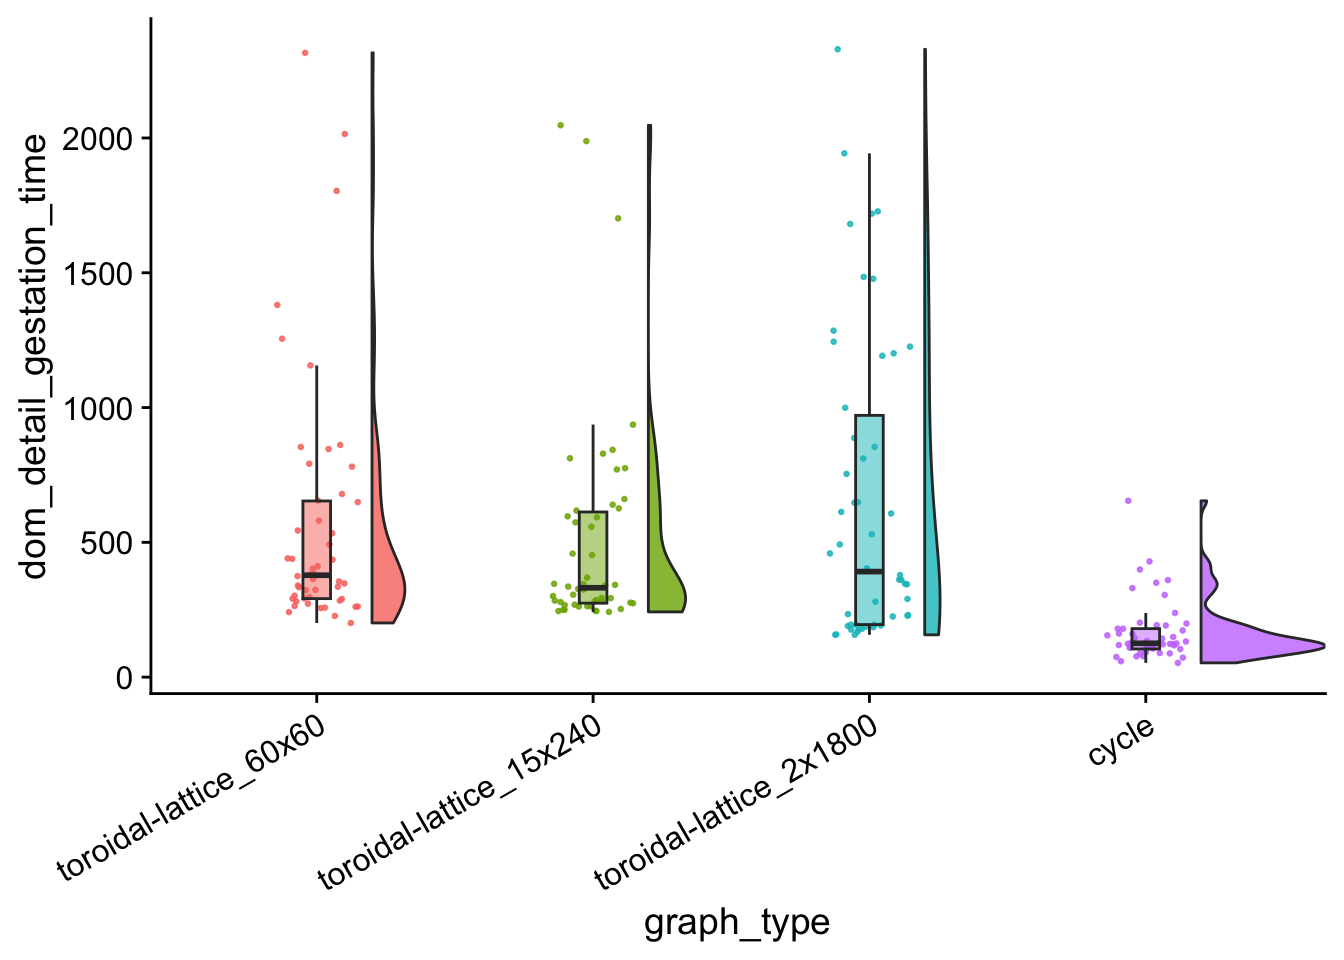
\includegraphics{supplemental-material_files/figure-latex/unnamed-chunk-92-1.pdf}

\begin{Shaded}
\begin{Highlighting}[]
\NormalTok{data }\SpecialCharTok{\%\textgreater{}\%}
  \FunctionTok{group\_by}\NormalTok{(graph\_type) }\SpecialCharTok{\%\textgreater{}\%}
  \FunctionTok{summarize}\NormalTok{(}
    \AttributeTok{reps =} \FunctionTok{n}\NormalTok{(),}
    \AttributeTok{median\_dom\_detail\_gestation\_time =} \FunctionTok{median}\NormalTok{(dom\_detail\_gestation\_time),}
    \AttributeTok{mean\_dom\_detail\_gestation\_time =} \FunctionTok{mean}\NormalTok{(dom\_detail\_gestation\_time)}
\NormalTok{  ) }\SpecialCharTok{\%\textgreater{}\%}
  \FunctionTok{arrange}\NormalTok{(}
    \FunctionTok{desc}\NormalTok{(mean\_dom\_detail\_gestation\_time)}
\NormalTok{  )}
\end{Highlighting}
\end{Shaded}

\begin{verbatim}
## # A tibble: 4 x 4
##   graph_type               reps median_dom_detail_gesta~1 mean_dom_detail_gest~2
##   <fct>                   <int>                     <dbl>                  <dbl>
## 1 toroidal-lattice_2x1800    50                      392.                   660.
## 2 toroidal-lattice_60x60     50                      378                    569.
## 3 toroidal-lattice_15x240    50                      332.                   508.
## 4 cycle                      50                      126.                   166.
## # i abbreviated names: 1: median_dom_detail_gestation_time,
## #   2: mean_dom_detail_gestation_time
\end{verbatim}

\begin{Shaded}
\begin{Highlighting}[]
\FunctionTok{kruskal.test}\NormalTok{(}
  \AttributeTok{formula =}\NormalTok{ dom\_detail\_gestation\_time }\SpecialCharTok{\textasciitilde{}}\NormalTok{ graph\_type,}
  \AttributeTok{data =}\NormalTok{ data}
\NormalTok{)}
\end{Highlighting}
\end{Shaded}

\begin{verbatim}
## 
##  Kruskal-Wallis rank sum test
## 
## data:  dom_detail_gestation_time by graph_type
## Kruskal-Wallis chi-squared = 77.537, df = 3, p-value < 2.2e-16
\end{verbatim}

\begin{Shaded}
\begin{Highlighting}[]
\NormalTok{wc\_results }\OtherTok{\textless{}{-}} \FunctionTok{pairwise.wilcox.test}\NormalTok{(}
  \AttributeTok{x =}\NormalTok{ data}\SpecialCharTok{$}\NormalTok{dom\_detail\_gestation\_time,}
  \AttributeTok{g =}\NormalTok{ data}\SpecialCharTok{$}\NormalTok{graph\_type,}
  \AttributeTok{p.adjust.method   =} \StringTok{"holm"}\NormalTok{,}
  \AttributeTok{exact =} \ConstantTok{FALSE}
\NormalTok{)}

\NormalTok{dom\_detail\_gestation\_time\_wc\_table }\OtherTok{\textless{}{-}} \FunctionTok{kbl}\NormalTok{(wc\_results}\SpecialCharTok{$}\NormalTok{p.value) }\SpecialCharTok{\%\textgreater{}\%} \FunctionTok{kable\_styling}\NormalTok{()}
\FunctionTok{save\_kable}\NormalTok{(dom\_detail\_gestation\_time\_wc\_table, }\FunctionTok{paste0}\NormalTok{(plot\_dir, }\StringTok{"/dom\_detail\_gestation\_time\_wc\_table.pdf"}\NormalTok{))}

\NormalTok{dom\_detail\_gestation\_time\_wc\_table}
\end{Highlighting}
\end{Shaded}

\begin{table}
\centering
\begin{tabular}[t]{l|r|r|r}
\hline
  & toroidal-lattice\_60x60 & toroidal-lattice\_15x240 & toroidal-lattice\_2x1800\\
\hline
toroidal-lattice\_15x240 & 0.8010941 & NA & NA\\
\hline
toroidal-lattice\_2x1800 & 1.0000000 & 1 & NA\\
\hline
cycle & 0.0000000 & 0 & 0\\
\hline
\end{tabular}
\end{table}

\hypertarget{dominant-genome-length-1}{%
\section{Dominant genome length}\label{dominant-genome-length-1}}

\begin{Shaded}
\begin{Highlighting}[]
\NormalTok{dom\_genome\_length\_plt }\OtherTok{\textless{}{-}} \FunctionTok{ggplot}\NormalTok{(}
    \AttributeTok{data =}\NormalTok{ data,}
    \AttributeTok{mapping =} \FunctionTok{aes}\NormalTok{(}
      \AttributeTok{x =}\NormalTok{ graph\_type,}
      \AttributeTok{y =}\NormalTok{ dom\_detail\_genome\_length,}
      \AttributeTok{fill =}\NormalTok{ graph\_type}
\NormalTok{    )}
\NormalTok{  ) }\SpecialCharTok{+}
  \FunctionTok{geom\_flat\_violin}\NormalTok{(}
    \AttributeTok{position =} \FunctionTok{position\_nudge}\NormalTok{(}\AttributeTok{x =}\NormalTok{ .}\DecValTok{2}\NormalTok{, }\AttributeTok{y =} \DecValTok{0}\NormalTok{),}
    \AttributeTok{alpha =}\NormalTok{ .}\DecValTok{8}
\NormalTok{  ) }\SpecialCharTok{+}
  \FunctionTok{geom\_point}\NormalTok{(}
    \AttributeTok{mapping=}\FunctionTok{aes}\NormalTok{(}\AttributeTok{color =}\NormalTok{ graph\_type),}
    \AttributeTok{position =} \FunctionTok{position\_jitter}\NormalTok{(}\AttributeTok{width =}\NormalTok{ .}\DecValTok{15}\NormalTok{),}
    \AttributeTok{size =}\NormalTok{ .}\DecValTok{5}\NormalTok{,}
    \AttributeTok{alpha =} \FloatTok{0.8}
\NormalTok{  ) }\SpecialCharTok{+}
  \FunctionTok{geom\_boxplot}\NormalTok{(}
    \AttributeTok{width =}\NormalTok{ .}\DecValTok{1}\NormalTok{,}
    \AttributeTok{outlier.shape =} \ConstantTok{NA}\NormalTok{,}
    \AttributeTok{alpha =} \FloatTok{0.5}
\NormalTok{  ) }\SpecialCharTok{+}
  \FunctionTok{theme}\NormalTok{(}
    \AttributeTok{legend.position =} \StringTok{"none"}\NormalTok{,}
    \AttributeTok{axis.text.x =} \FunctionTok{element\_text}\NormalTok{(}
      \AttributeTok{angle =} \DecValTok{30}\NormalTok{,}
      \AttributeTok{hjust =} \DecValTok{1}
\NormalTok{    )}
\NormalTok{  )}

\FunctionTok{ggsave}\NormalTok{(}
  \AttributeTok{filename =} \FunctionTok{paste0}\NormalTok{(plot\_dir, }\StringTok{"/dom\_genome\_length.pdf"}\NormalTok{),}
  \AttributeTok{plot =}\NormalTok{ dom\_genome\_length\_plt,}
  \AttributeTok{width =} \DecValTok{15}\NormalTok{,}
  \AttributeTok{height =} \DecValTok{10}
\NormalTok{)}

\NormalTok{dom\_genome\_length\_plt}
\end{Highlighting}
\end{Shaded}

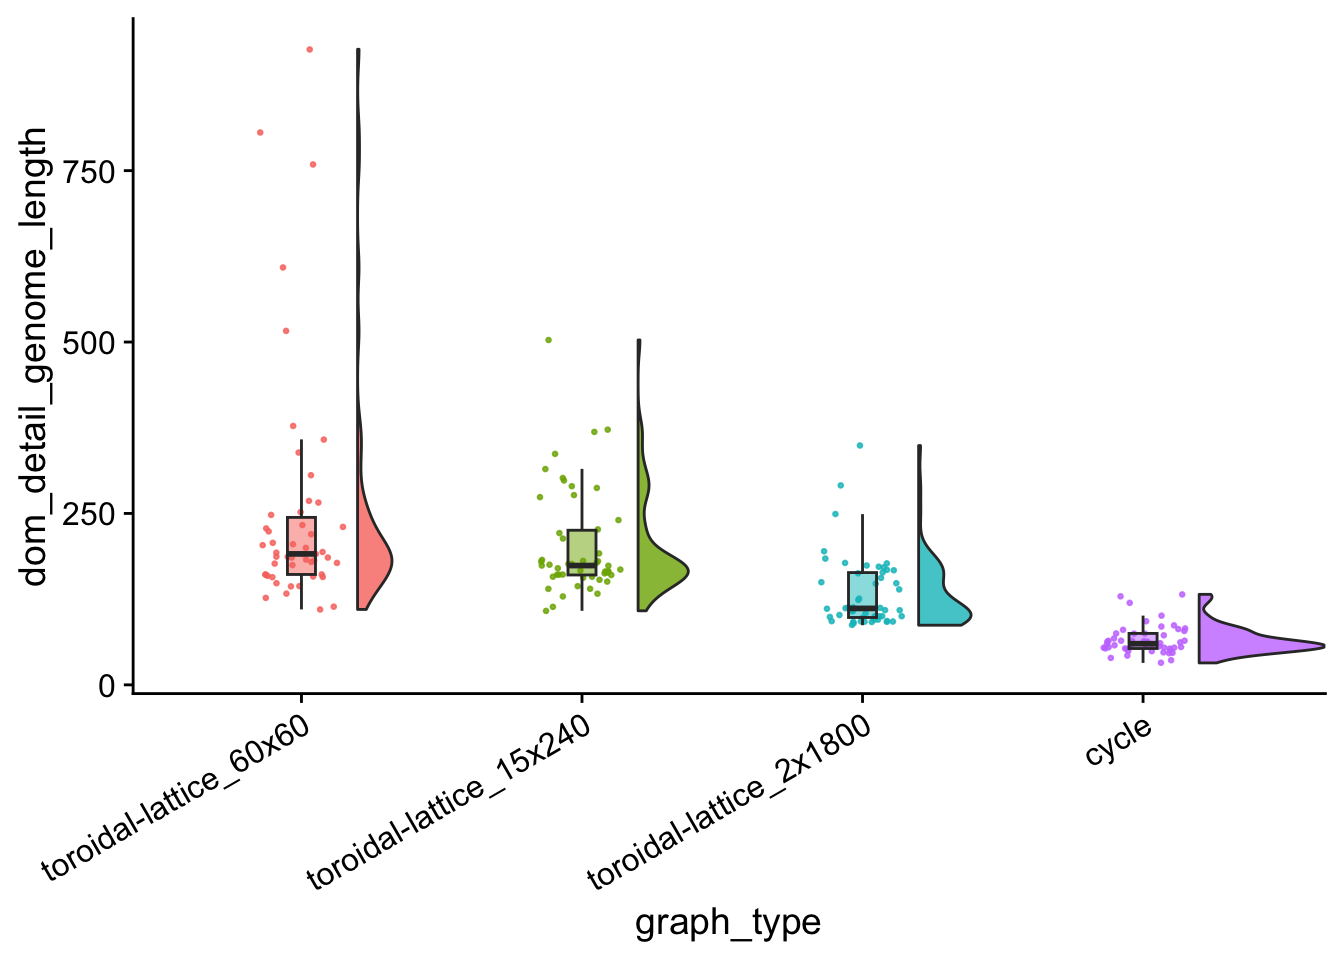
\includegraphics{supplemental-material_files/figure-latex/unnamed-chunk-95-1.pdf}

\begin{Shaded}
\begin{Highlighting}[]
\NormalTok{data }\SpecialCharTok{\%\textgreater{}\%}
  \FunctionTok{group\_by}\NormalTok{(graph\_type) }\SpecialCharTok{\%\textgreater{}\%}
  \FunctionTok{summarize}\NormalTok{(}
    \AttributeTok{reps =} \FunctionTok{n}\NormalTok{(),}
    \AttributeTok{median\_dom\_detail\_genome\_length =} \FunctionTok{median}\NormalTok{(dom\_detail\_genome\_length),}
    \AttributeTok{mean\_dom\_detail\_genome\_length =} \FunctionTok{mean}\NormalTok{(dom\_detail\_genome\_length)}
\NormalTok{  ) }\SpecialCharTok{\%\textgreater{}\%}
  \FunctionTok{arrange}\NormalTok{(}
    \FunctionTok{desc}\NormalTok{(mean\_dom\_detail\_genome\_length)}
\NormalTok{  )}
\end{Highlighting}
\end{Shaded}

\begin{verbatim}
## # A tibble: 4 x 4
##   graph_type               reps median_dom_detail_genom~1 mean_dom_detail_geno~2
##   <fct>                   <int>                     <dbl>                  <dbl>
## 1 toroidal-lattice_60x60     50                      191                   252. 
## 2 toroidal-lattice_15x240    50                      174                   203. 
## 3 toroidal-lattice_2x1800    50                      112.                  134. 
## 4 cycle                      50                       60                    65.4
## # i abbreviated names: 1: median_dom_detail_genome_length,
## #   2: mean_dom_detail_genome_length
\end{verbatim}

\begin{Shaded}
\begin{Highlighting}[]
\FunctionTok{kruskal.test}\NormalTok{(}
  \AttributeTok{formula =}\NormalTok{ dom\_detail\_genome\_length }\SpecialCharTok{\textasciitilde{}}\NormalTok{ graph\_type,}
  \AttributeTok{data =}\NormalTok{ data}
\NormalTok{)}
\end{Highlighting}
\end{Shaded}

\begin{verbatim}
## 
##  Kruskal-Wallis rank sum test
## 
## data:  dom_detail_genome_length by graph_type
## Kruskal-Wallis chi-squared = 133.54, df = 3, p-value < 2.2e-16
\end{verbatim}

\begin{Shaded}
\begin{Highlighting}[]
\NormalTok{wc\_results }\OtherTok{\textless{}{-}} \FunctionTok{pairwise.wilcox.test}\NormalTok{(}
  \AttributeTok{x =}\NormalTok{ data}\SpecialCharTok{$}\NormalTok{dom\_detail\_genome\_length,}
  \AttributeTok{g =}\NormalTok{ data}\SpecialCharTok{$}\NormalTok{graph\_type,}
  \AttributeTok{p.adjust.method   =} \StringTok{"holm"}\NormalTok{,}
  \AttributeTok{exact =} \ConstantTok{FALSE}
\NormalTok{)}

\NormalTok{dom\_detail\_genome\_length\_wc\_table }\OtherTok{\textless{}{-}} \FunctionTok{kbl}\NormalTok{(wc\_results}\SpecialCharTok{$}\NormalTok{p.value) }\SpecialCharTok{\%\textgreater{}\%} \FunctionTok{kable\_styling}\NormalTok{()}
\FunctionTok{save\_kable}\NormalTok{(dom\_detail\_genome\_length\_wc\_table, }\FunctionTok{paste0}\NormalTok{(plot\_dir, }\StringTok{"/dom\_detail\_genome\_length\_wc\_table.pdf"}\NormalTok{))}

\NormalTok{dom\_detail\_genome\_length\_wc\_table}
\end{Highlighting}
\end{Shaded}

\begin{table}
\centering
\begin{tabular}[t]{l|r|r|r}
\hline
  & toroidal-lattice\_60x60 & toroidal-lattice\_15x240 & toroidal-lattice\_2x1800\\
\hline
toroidal-lattice\_15x240 & 0.0972676 & NA & NA\\
\hline
toroidal-lattice\_2x1800 & 0.0000000 & 1e-07 & NA\\
\hline
cycle & 0.0000000 & 0e+00 & 0\\
\hline
\end{tabular}
\end{table}

\hypertarget{task-profile-entropy-1}{%
\section{Task profile entropy}\label{task-profile-entropy-1}}

\begin{Shaded}
\begin{Highlighting}[]
\NormalTok{task\_profile\_entropy\_plt }\OtherTok{\textless{}{-}} \FunctionTok{ggplot}\NormalTok{(}
    \AttributeTok{data =}\NormalTok{ data,}
    \AttributeTok{mapping =} \FunctionTok{aes}\NormalTok{(}
      \AttributeTok{x =}\NormalTok{ graph\_type,}
      \AttributeTok{y =}\NormalTok{ task\_profile\_entropy,}
      \AttributeTok{fill =}\NormalTok{ graph\_type}
\NormalTok{    )}
\NormalTok{  ) }\SpecialCharTok{+}
  \FunctionTok{geom\_flat\_violin}\NormalTok{(}
    \AttributeTok{position =} \FunctionTok{position\_nudge}\NormalTok{(}\AttributeTok{x =}\NormalTok{ .}\DecValTok{2}\NormalTok{, }\AttributeTok{y =} \DecValTok{0}\NormalTok{),}
    \AttributeTok{alpha =}\NormalTok{ .}\DecValTok{8}
\NormalTok{  ) }\SpecialCharTok{+}
  \FunctionTok{geom\_point}\NormalTok{(}
    \AttributeTok{mapping=}\FunctionTok{aes}\NormalTok{(}\AttributeTok{color =}\NormalTok{ graph\_type),}
    \AttributeTok{position =} \FunctionTok{position\_jitter}\NormalTok{(}\AttributeTok{width =}\NormalTok{ .}\DecValTok{15}\NormalTok{),}
    \AttributeTok{size =}\NormalTok{ .}\DecValTok{5}\NormalTok{,}
    \AttributeTok{alpha =} \FloatTok{0.8}
\NormalTok{  ) }\SpecialCharTok{+}
  \FunctionTok{geom\_boxplot}\NormalTok{(}
    \AttributeTok{width =}\NormalTok{ .}\DecValTok{1}\NormalTok{,}
    \AttributeTok{outlier.shape =} \ConstantTok{NA}\NormalTok{,}
    \AttributeTok{alpha =} \FloatTok{0.5}
\NormalTok{  ) }\SpecialCharTok{+}
  \FunctionTok{theme}\NormalTok{(}
    \AttributeTok{legend.position =} \StringTok{"none"}\NormalTok{,}
    \AttributeTok{axis.text.x =} \FunctionTok{element\_text}\NormalTok{(}
      \AttributeTok{angle =} \DecValTok{30}\NormalTok{,}
      \AttributeTok{hjust =} \DecValTok{1}
\NormalTok{    )}
\NormalTok{  )}

\FunctionTok{ggsave}\NormalTok{(}
  \AttributeTok{filename =} \FunctionTok{paste0}\NormalTok{(plot\_dir, }\StringTok{"/task\_profile\_entropy.pdf"}\NormalTok{),}
  \AttributeTok{plot =}\NormalTok{ task\_profile\_entropy\_plt,}
  \AttributeTok{width =} \DecValTok{15}\NormalTok{,}
  \AttributeTok{height =} \DecValTok{10}
\NormalTok{)}

\NormalTok{task\_profile\_entropy\_plt}
\end{Highlighting}
\end{Shaded}

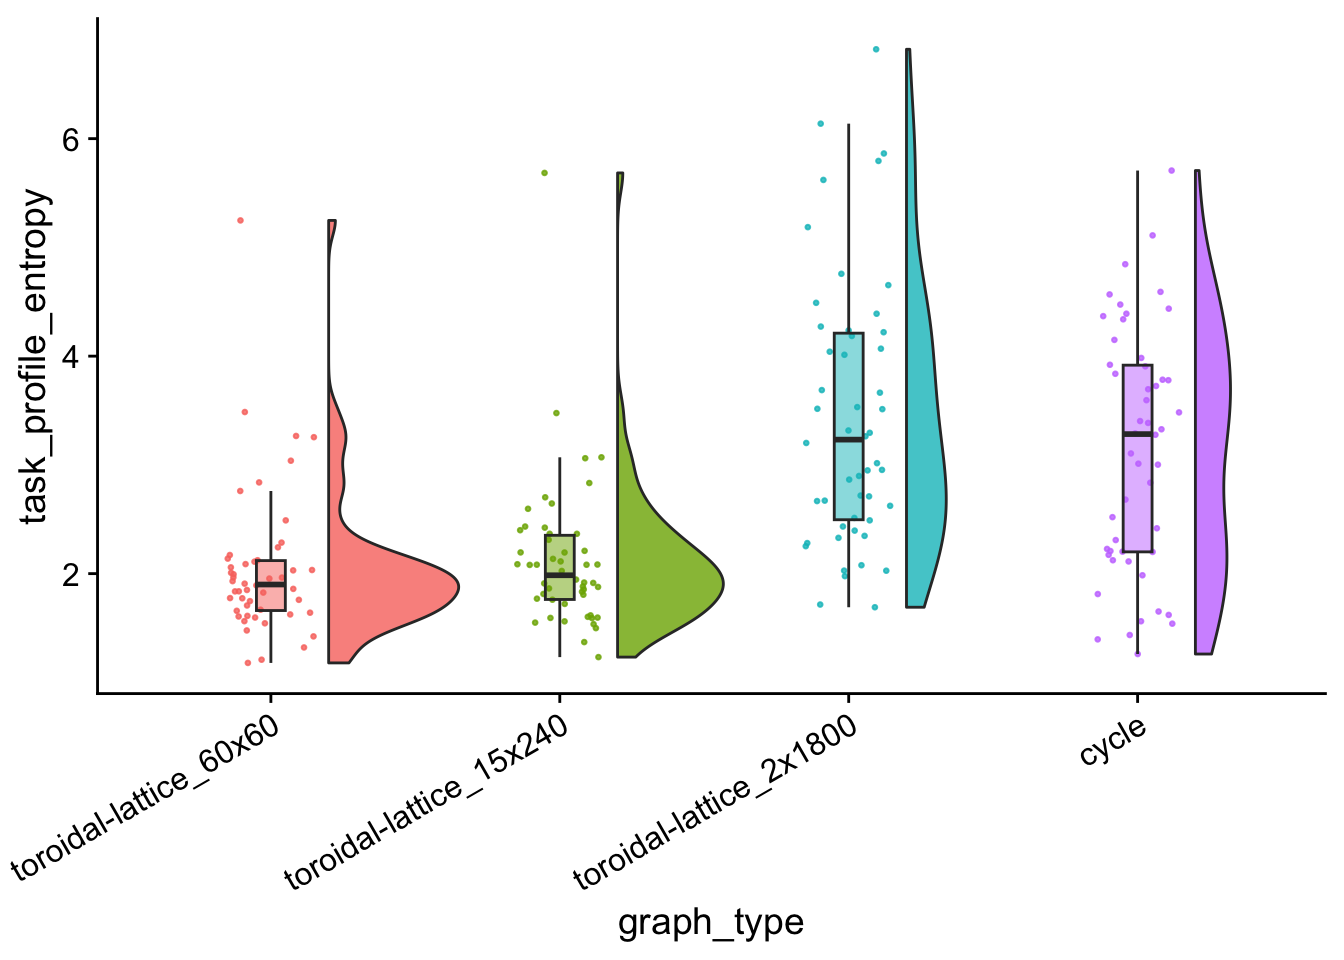
\includegraphics{supplemental-material_files/figure-latex/unnamed-chunk-98-1.pdf}

\begin{Shaded}
\begin{Highlighting}[]
\NormalTok{task\_profile\_count\_plt }\OtherTok{\textless{}{-}} \FunctionTok{ggplot}\NormalTok{(}
    \AttributeTok{data =}\NormalTok{ data,}
    \AttributeTok{mapping =} \FunctionTok{aes}\NormalTok{(}
      \AttributeTok{x =}\NormalTok{ graph\_type,}
      \AttributeTok{y =}\NormalTok{ task\_profile\_count,}
      \AttributeTok{fill =}\NormalTok{ graph\_type}
\NormalTok{    )}
\NormalTok{  ) }\SpecialCharTok{+}
  \FunctionTok{geom\_flat\_violin}\NormalTok{(}
    \AttributeTok{position =} \FunctionTok{position\_nudge}\NormalTok{(}\AttributeTok{x =}\NormalTok{ .}\DecValTok{2}\NormalTok{, }\AttributeTok{y =} \DecValTok{0}\NormalTok{),}
    \AttributeTok{alpha =}\NormalTok{ .}\DecValTok{8}
\NormalTok{  ) }\SpecialCharTok{+}
  \FunctionTok{geom\_point}\NormalTok{(}
    \AttributeTok{mapping=}\FunctionTok{aes}\NormalTok{(}\AttributeTok{color =}\NormalTok{ graph\_type),}
    \AttributeTok{position =} \FunctionTok{position\_jitter}\NormalTok{(}\AttributeTok{width =}\NormalTok{ .}\DecValTok{15}\NormalTok{),}
    \AttributeTok{size =}\NormalTok{ .}\DecValTok{5}\NormalTok{,}
    \AttributeTok{alpha =} \FloatTok{0.8}
\NormalTok{  ) }\SpecialCharTok{+}
  \FunctionTok{geom\_boxplot}\NormalTok{(}
    \AttributeTok{width =}\NormalTok{ .}\DecValTok{1}\NormalTok{,}
    \AttributeTok{outlier.shape =} \ConstantTok{NA}\NormalTok{,}
    \AttributeTok{alpha =} \FloatTok{0.5}
\NormalTok{  ) }\SpecialCharTok{+}
  \FunctionTok{theme}\NormalTok{(}
    \AttributeTok{legend.position =} \StringTok{"none"}\NormalTok{,}
    \AttributeTok{axis.text.x =} \FunctionTok{element\_text}\NormalTok{(}
      \AttributeTok{angle =} \DecValTok{30}\NormalTok{,}
      \AttributeTok{hjust =} \DecValTok{1}
\NormalTok{    )}
\NormalTok{  )}

\FunctionTok{ggsave}\NormalTok{(}
  \AttributeTok{filename =} \FunctionTok{paste0}\NormalTok{(plot\_dir, }\StringTok{"/task\_profile\_count.pdf"}\NormalTok{),}
  \AttributeTok{plot =}\NormalTok{ task\_profile\_count\_plt,}
  \AttributeTok{width =} \DecValTok{15}\NormalTok{,}
  \AttributeTok{height =} \DecValTok{10}
\NormalTok{)}

\NormalTok{task\_profile\_count\_plt}
\end{Highlighting}
\end{Shaded}

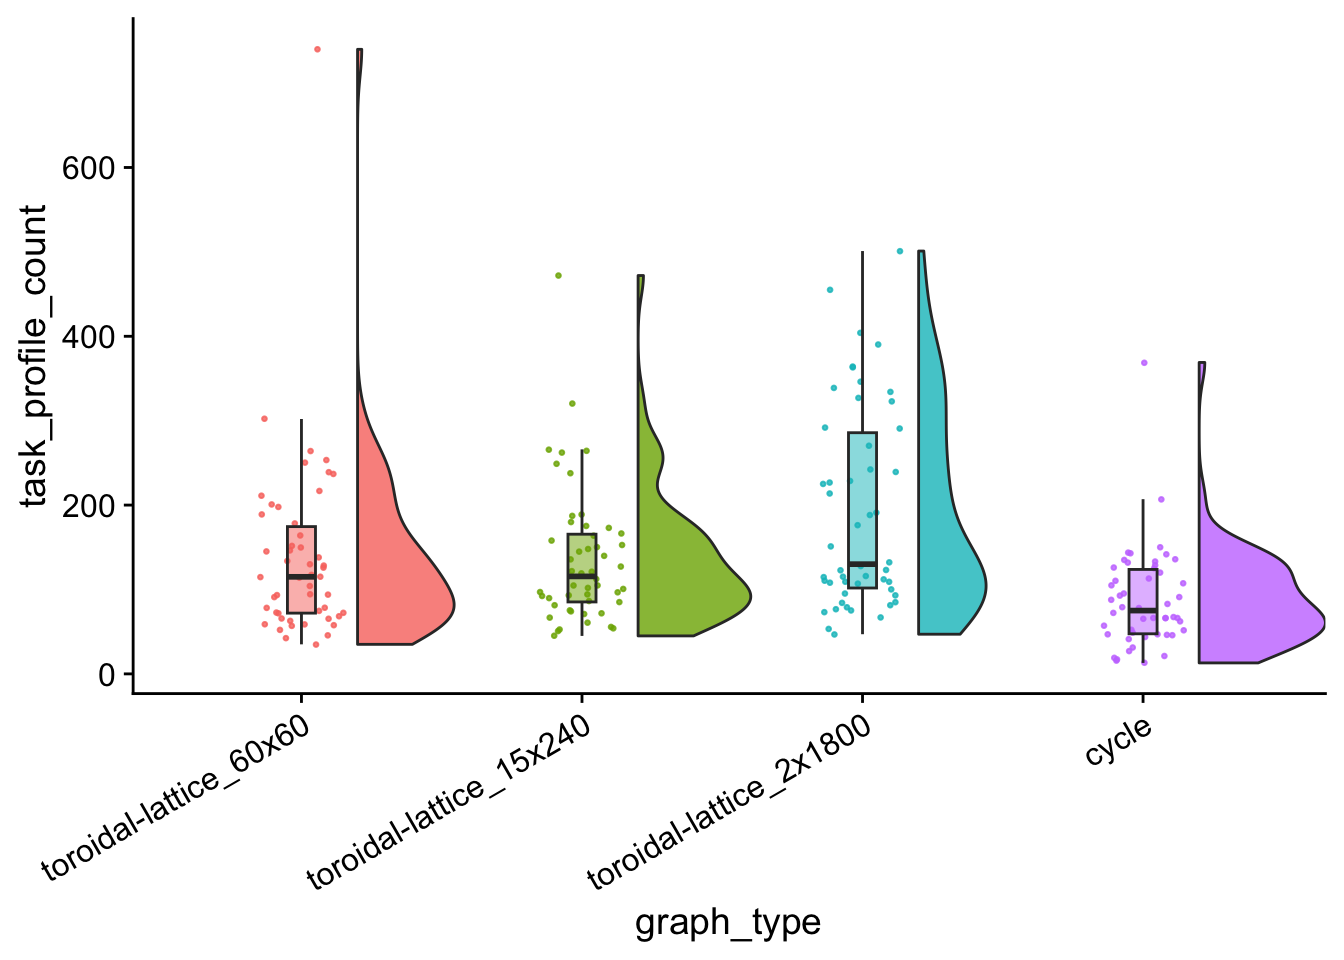
\includegraphics{supplemental-material_files/figure-latex/unnamed-chunk-99-1.pdf}

\hypertarget{average-generation-1}{%
\section{Average generation}\label{average-generation-1}}

\begin{Shaded}
\begin{Highlighting}[]
\NormalTok{avg\_generation\_plt }\OtherTok{\textless{}{-}} \FunctionTok{ggplot}\NormalTok{(}
    \AttributeTok{data =}\NormalTok{ data,}
    \AttributeTok{mapping =} \FunctionTok{aes}\NormalTok{(}
      \AttributeTok{x =}\NormalTok{ graph\_type,}
      \AttributeTok{y =}\NormalTok{ time\_average\_generation,}
      \AttributeTok{fill =}\NormalTok{ graph\_type}
\NormalTok{    )}
\NormalTok{  ) }\SpecialCharTok{+}
  \FunctionTok{geom\_flat\_violin}\NormalTok{(}
    \AttributeTok{position =} \FunctionTok{position\_nudge}\NormalTok{(}\AttributeTok{x =}\NormalTok{ .}\DecValTok{2}\NormalTok{, }\AttributeTok{y =} \DecValTok{0}\NormalTok{),}
    \AttributeTok{alpha =}\NormalTok{ .}\DecValTok{8}
\NormalTok{  ) }\SpecialCharTok{+}
  \FunctionTok{geom\_point}\NormalTok{(}
    \AttributeTok{mapping=}\FunctionTok{aes}\NormalTok{(}\AttributeTok{color =}\NormalTok{ graph\_type),}
    \AttributeTok{position =} \FunctionTok{position\_jitter}\NormalTok{(}\AttributeTok{width =}\NormalTok{ .}\DecValTok{15}\NormalTok{),}
    \AttributeTok{size =}\NormalTok{ .}\DecValTok{5}\NormalTok{,}
    \AttributeTok{alpha =} \FloatTok{0.8}
\NormalTok{  ) }\SpecialCharTok{+}
  \FunctionTok{geom\_boxplot}\NormalTok{(}
    \AttributeTok{width =}\NormalTok{ .}\DecValTok{1}\NormalTok{,}
    \AttributeTok{outlier.shape =} \ConstantTok{NA}\NormalTok{,}
    \AttributeTok{alpha =} \FloatTok{0.5}
\NormalTok{  ) }\SpecialCharTok{+}
  \FunctionTok{theme}\NormalTok{(}
    \AttributeTok{legend.position =} \StringTok{"none"}\NormalTok{,}
    \AttributeTok{axis.text.x =} \FunctionTok{element\_text}\NormalTok{(}
      \AttributeTok{angle =} \DecValTok{30}\NormalTok{,}
      \AttributeTok{hjust =} \DecValTok{1}
\NormalTok{    )}
\NormalTok{  )}

\FunctionTok{ggsave}\NormalTok{(}
  \AttributeTok{filename =} \FunctionTok{paste0}\NormalTok{(plot\_dir, }\StringTok{"/avg\_generation.pdf"}\NormalTok{),}
  \AttributeTok{plot =}\NormalTok{ avg\_generation\_plt,}
  \AttributeTok{width =} \DecValTok{15}\NormalTok{,}
  \AttributeTok{height =} \DecValTok{10}
\NormalTok{)}

\NormalTok{avg\_generation\_plt}
\end{Highlighting}
\end{Shaded}

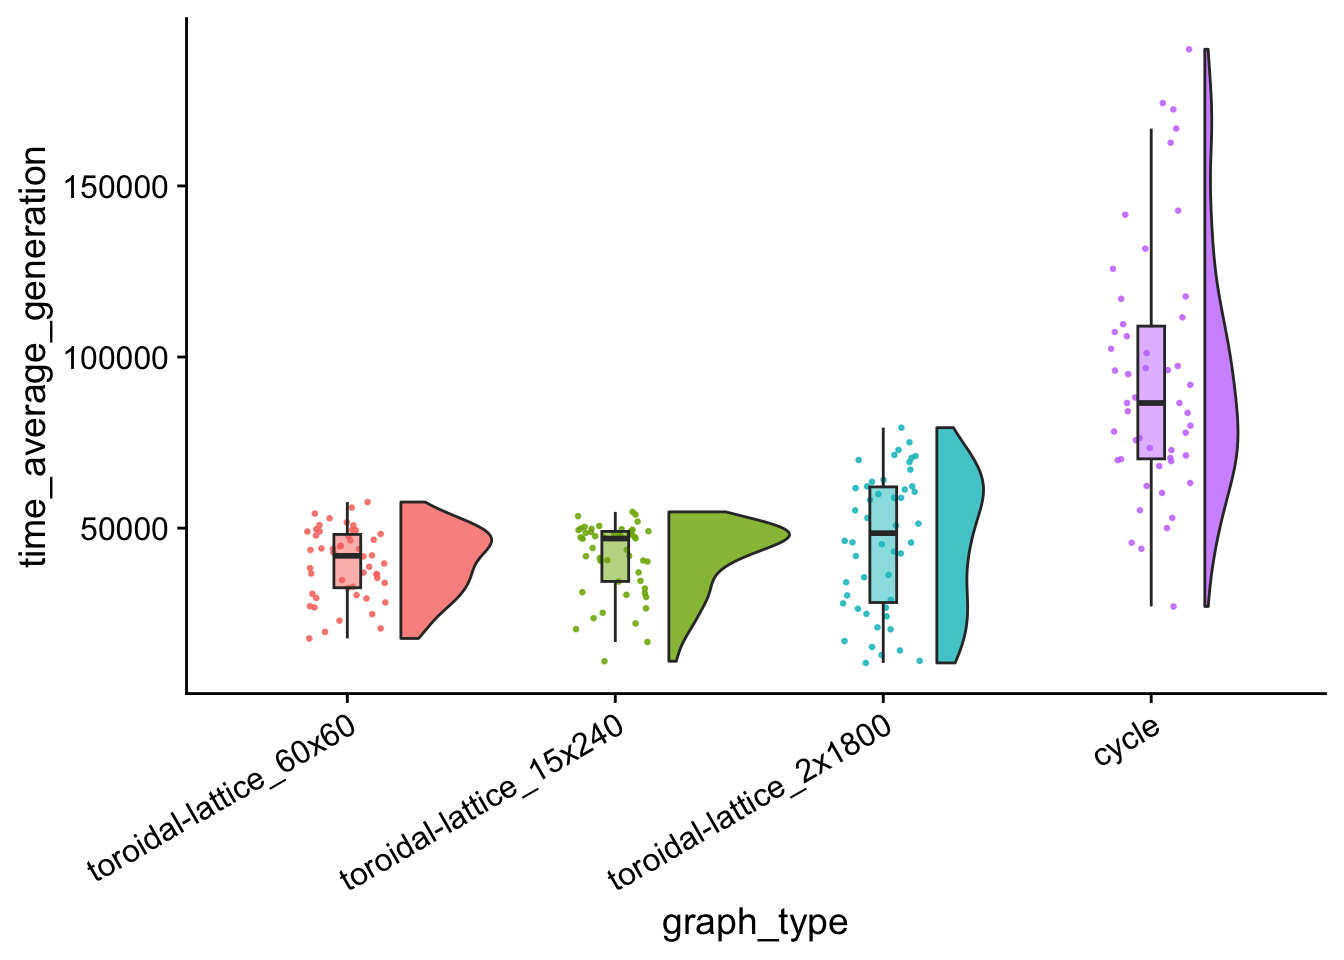
\includegraphics{supplemental-material_files/figure-latex/unnamed-chunk-100-1.pdf}

\begin{Shaded}
\begin{Highlighting}[]
\NormalTok{data }\SpecialCharTok{\%\textgreater{}\%}
  \FunctionTok{group\_by}\NormalTok{(graph\_type) }\SpecialCharTok{\%\textgreater{}\%}
  \FunctionTok{summarize}\NormalTok{(}
    \AttributeTok{reps =} \FunctionTok{n}\NormalTok{(),}
    \AttributeTok{median\_time\_average\_generation =} \FunctionTok{median}\NormalTok{(time\_average\_generation),}
    \AttributeTok{mean\_time\_average\_generation =} \FunctionTok{mean}\NormalTok{(time\_average\_generation)}
\NormalTok{  ) }\SpecialCharTok{\%\textgreater{}\%}
  \FunctionTok{arrange}\NormalTok{(}
    \FunctionTok{desc}\NormalTok{(mean\_time\_average\_generation)}
\NormalTok{  )}
\end{Highlighting}
\end{Shaded}

\begin{verbatim}
## # A tibble: 4 x 4
##   graph_type               reps median_time_average_gen~1 mean_time_average_ge~2
##   <fct>                   <int>                     <dbl>                  <dbl>
## 1 cycle                      50                    86561.                 93949.
## 2 toroidal-lattice_2x1800    50                    48531.                 46331.
## 3 toroidal-lattice_15x240    50                    46955.                 41302.
## 4 toroidal-lattice_60x60     50                    41905.                 39813.
## # i abbreviated names: 1: median_time_average_generation,
## #   2: mean_time_average_generation
\end{verbatim}

\hypertarget{population-task-count-over-time-1}{%
\section{Population task count over time}\label{population-task-count-over-time-1}}

\begin{Shaded}
\begin{Highlighting}[]
\NormalTok{pop\_task\_cnt\_ts }\OtherTok{\textless{}{-}} \FunctionTok{ggplot}\NormalTok{(}
    \AttributeTok{data =}\NormalTok{ time\_series\_data,}
    \AttributeTok{mapping =} \FunctionTok{aes}\NormalTok{(}
      \AttributeTok{x =}\NormalTok{ update,}
      \AttributeTok{y =}\NormalTok{ pop\_task\_total\_tasks\_done,}
      \AttributeTok{color =}\NormalTok{ graph\_type,}
      \AttributeTok{fill =}\NormalTok{ graph\_type}
\NormalTok{    )}
\NormalTok{  ) }\SpecialCharTok{+}
  \FunctionTok{stat\_summary}\NormalTok{(}\AttributeTok{fun =} \StringTok{"mean"}\NormalTok{, }\AttributeTok{geom =} \StringTok{"line"}\NormalTok{) }\SpecialCharTok{+}
  \FunctionTok{stat\_summary}\NormalTok{(}
    \AttributeTok{fun.data =} \StringTok{"mean\_cl\_boot"}\NormalTok{,}
    \AttributeTok{fun.args =} \FunctionTok{list}\NormalTok{(}\AttributeTok{conf.int =} \FloatTok{0.95}\NormalTok{),}
    \AttributeTok{geom =} \StringTok{"ribbon"}\NormalTok{,}
    \AttributeTok{alpha =} \FloatTok{0.2}\NormalTok{,}
    \AttributeTok{linetype =} \DecValTok{0}
\NormalTok{  ) }\SpecialCharTok{+}
  \FunctionTok{theme}\NormalTok{(}\AttributeTok{legend.position =} \StringTok{"bottom"}\NormalTok{)}

\FunctionTok{ggsave}\NormalTok{(}
  \AttributeTok{plot =}\NormalTok{ pop\_task\_cnt\_ts,}
  \AttributeTok{filename =} \FunctionTok{paste0}\NormalTok{(}
\NormalTok{    working\_directory,}
    \StringTok{"/plots/pop\_tasks\_ts.pdf"}
\NormalTok{  ),}
  \AttributeTok{width =} \DecValTok{15}\NormalTok{,}
  \AttributeTok{height =} \DecValTok{10}
\NormalTok{)}

\NormalTok{pop\_task\_cnt\_ts}
\end{Highlighting}
\end{Shaded}

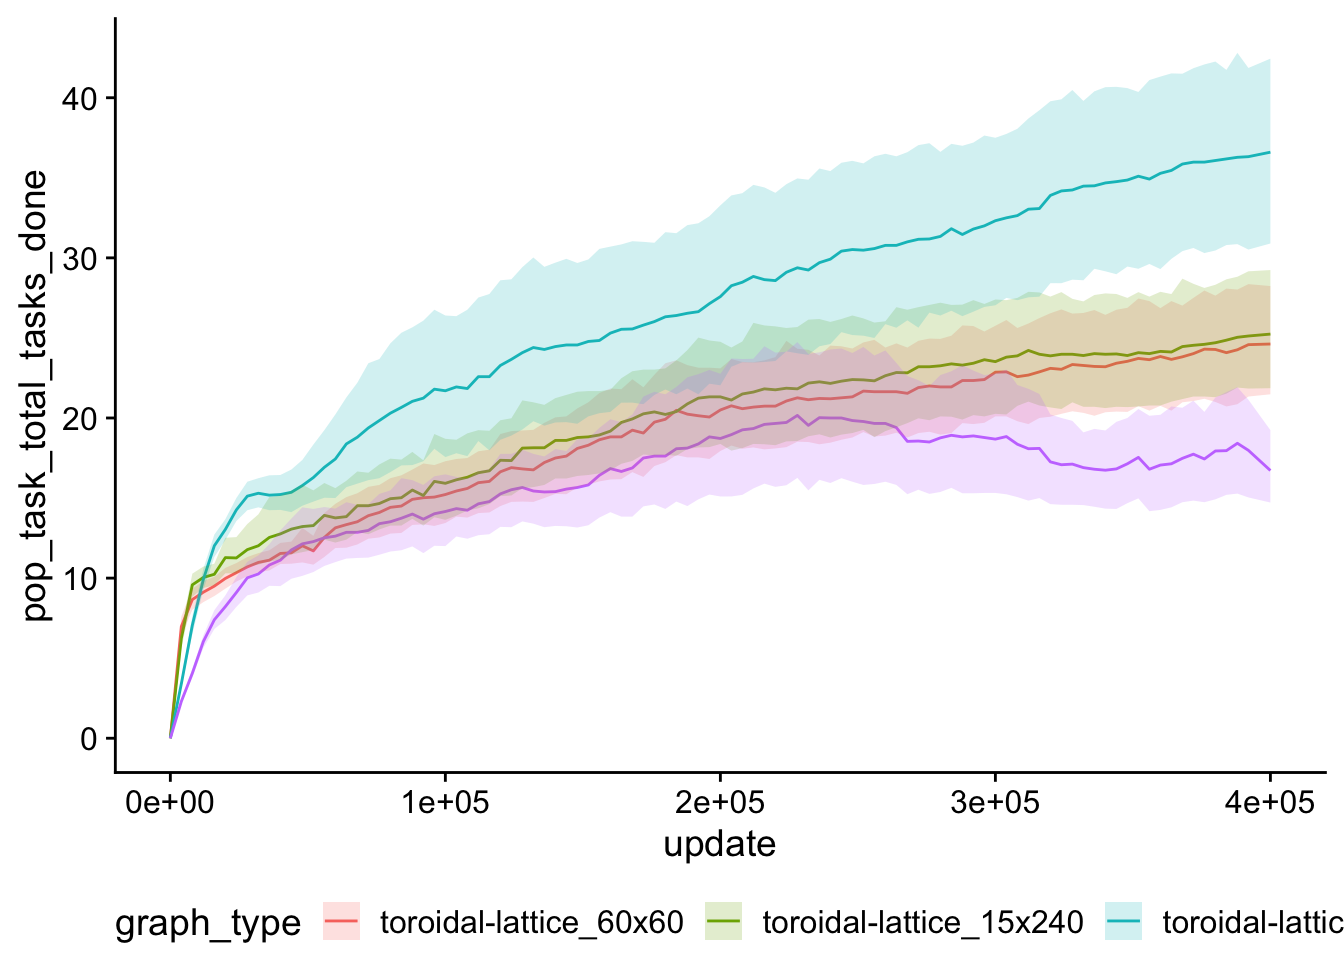
\includegraphics{supplemental-material_files/figure-latex/unnamed-chunk-102-1.pdf}

\hypertarget{average-generation-over-time-1}{%
\section{Average generation over time}\label{average-generation-over-time-1}}

\begin{Shaded}
\begin{Highlighting}[]
\NormalTok{time\_average\_generation\_ts }\OtherTok{\textless{}{-}} \FunctionTok{ggplot}\NormalTok{(}
    \AttributeTok{data =}\NormalTok{ time\_series\_data,}
    \AttributeTok{mapping =} \FunctionTok{aes}\NormalTok{(}
      \AttributeTok{x =}\NormalTok{ update,}
      \AttributeTok{y =}\NormalTok{ time\_average\_generation,}
      \AttributeTok{color =}\NormalTok{ graph\_type,}
      \AttributeTok{fill =}\NormalTok{ graph\_type}
\NormalTok{    )}
\NormalTok{  ) }\SpecialCharTok{+}
  \FunctionTok{stat\_summary}\NormalTok{(}\AttributeTok{fun =} \StringTok{"mean"}\NormalTok{, }\AttributeTok{geom =} \StringTok{"line"}\NormalTok{) }\SpecialCharTok{+}
  \FunctionTok{stat\_summary}\NormalTok{(}
    \AttributeTok{fun.data =} \StringTok{"mean\_cl\_boot"}\NormalTok{,}
    \AttributeTok{fun.args =} \FunctionTok{list}\NormalTok{(}\AttributeTok{conf.int =} \FloatTok{0.95}\NormalTok{),}
    \AttributeTok{geom =} \StringTok{"ribbon"}\NormalTok{,}
    \AttributeTok{alpha =} \FloatTok{0.2}\NormalTok{,}
    \AttributeTok{linetype =} \DecValTok{0}
\NormalTok{  ) }\SpecialCharTok{+}
  \FunctionTok{facet\_wrap}\NormalTok{(}\SpecialCharTok{\textasciitilde{}}\NormalTok{ENVIRONMENT\_FILE) }\SpecialCharTok{+}
  \FunctionTok{theme}\NormalTok{(}\AttributeTok{legend.position =} \StringTok{"bottom"}\NormalTok{)}

\FunctionTok{ggsave}\NormalTok{(}
  \AttributeTok{plot =}\NormalTok{ time\_average\_generation\_ts,}
  \AttributeTok{filename =} \FunctionTok{paste0}\NormalTok{(}
\NormalTok{    working\_directory,}
    \StringTok{"/plots/time\_average\_generation\_ts.pdf"}
\NormalTok{  ),}
  \AttributeTok{width =} \DecValTok{15}\NormalTok{,}
  \AttributeTok{height =} \DecValTok{10}
\NormalTok{)}

\NormalTok{time\_average\_generation\_ts}
\end{Highlighting}
\end{Shaded}

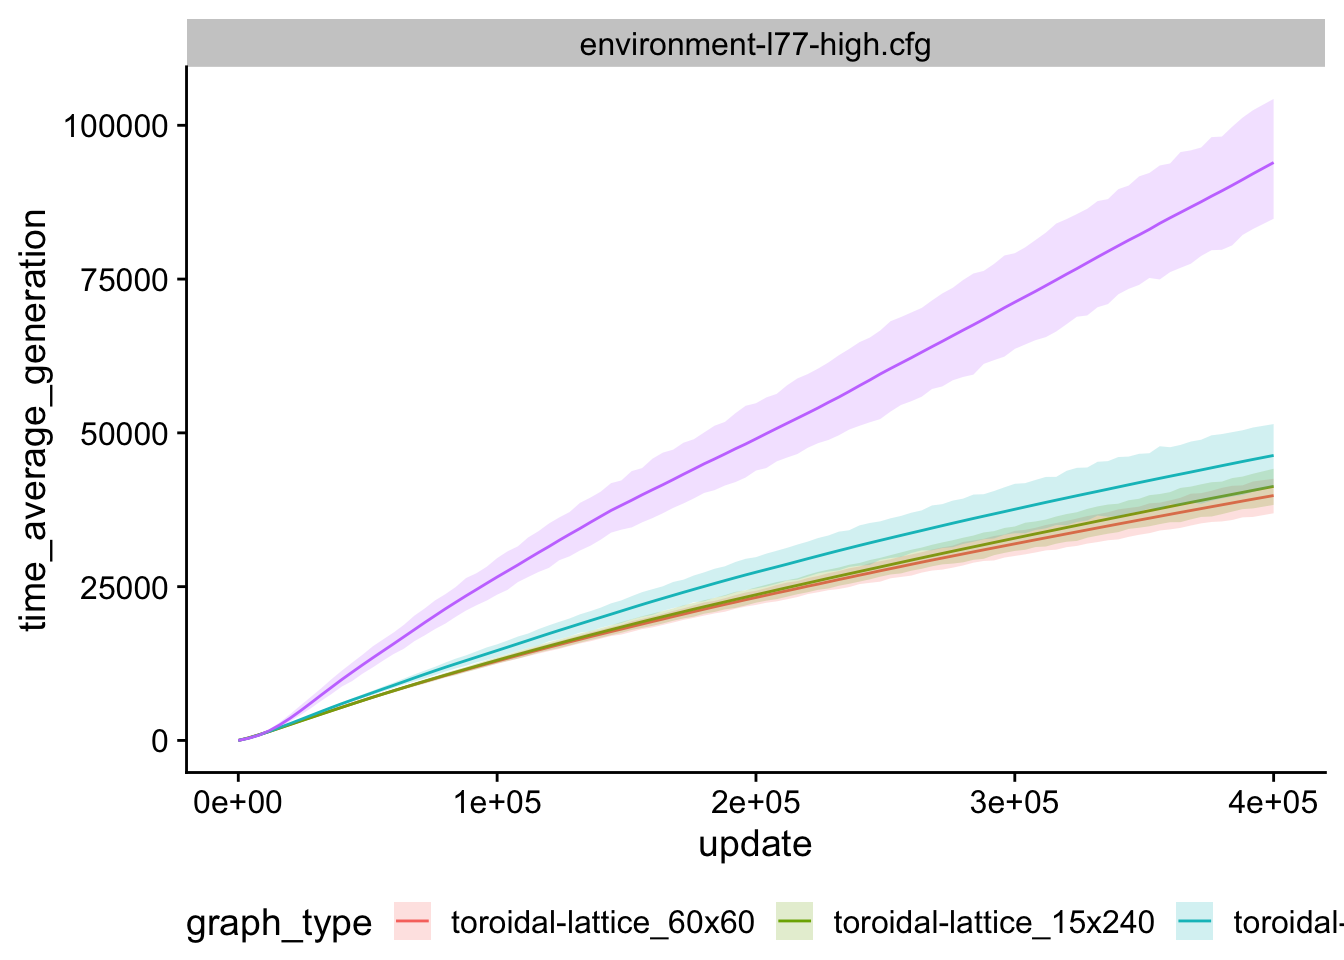
\includegraphics{supplemental-material_files/figure-latex/unnamed-chunk-103-1.pdf}

\hypertarget{graph-location-info-1}{%
\section{Graph location info}\label{graph-location-info-1}}

Analyze graph\_birth\_info\_annotated.csv

\begin{Shaded}
\begin{Highlighting}[]
\CommentTok{\# Load summary data from final update}
\NormalTok{graph\_loc\_data\_path }\OtherTok{\textless{}{-}} \FunctionTok{paste}\NormalTok{(}
\NormalTok{  working\_directory,}
  \StringTok{"data"}\NormalTok{,}
  \StringTok{"graph\_birth\_info\_annotated.csv"}\NormalTok{,}
  \AttributeTok{sep =} \StringTok{"/"}
\NormalTok{)}
\NormalTok{graph\_loc\_data }\OtherTok{\textless{}{-}} \FunctionTok{read\_csv}\NormalTok{(graph\_loc\_data\_path)}

\NormalTok{graph\_loc\_data }\OtherTok{\textless{}{-}}\NormalTok{ graph\_loc\_data }\SpecialCharTok{\%\textgreater{}\%}
  \FunctionTok{mutate}\NormalTok{(}
    \AttributeTok{graph\_type =} \FunctionTok{factor}\NormalTok{(}
\NormalTok{      graph\_type,}
      \AttributeTok{levels =} \FunctionTok{c}\NormalTok{(}
        \StringTok{"toroidal{-}lattice\_60x60"}\NormalTok{,}
        \StringTok{"toroidal{-}lattice\_30x120"}\NormalTok{,}
        \StringTok{"toroidal{-}lattice\_15x240"}\NormalTok{,}
        \StringTok{"toroidal{-}lattice\_4x900"}\NormalTok{,}
        \StringTok{"toroidal{-}lattice\_3x1200"}\NormalTok{,}
        \StringTok{"toroidal{-}lattice\_2x1800"}\NormalTok{,}
        \StringTok{"cycle"}
\NormalTok{      )}
\NormalTok{    ),}
    \AttributeTok{seed =} \FunctionTok{as.factor}\NormalTok{(seed)}
\NormalTok{  ) }\SpecialCharTok{\%\textgreater{}\%}
  \FunctionTok{filter}\NormalTok{(}
\NormalTok{    graph\_type }\SpecialCharTok{\%in\%}\NormalTok{ focal\_graphs}
\NormalTok{  )}
\end{Highlighting}
\end{Shaded}

Summarize by seed

\begin{Shaded}
\begin{Highlighting}[]
\NormalTok{graph\_loc\_data\_summary }\OtherTok{\textless{}{-}}\NormalTok{ graph\_loc\_data }\SpecialCharTok{\%\textgreater{}\%}
  \FunctionTok{group\_by}\NormalTok{(seed, graph\_type) }\SpecialCharTok{\%\textgreater{}\%}
  \FunctionTok{summarize}\NormalTok{(}
    \AttributeTok{births\_var =} \FunctionTok{var}\NormalTok{(births),}
    \AttributeTok{births\_total =} \FunctionTok{sum}\NormalTok{(births),}
    \AttributeTok{task\_apps\_total =} \FunctionTok{sum}\NormalTok{(task\_appearances),}
    \AttributeTok{task\_apps\_var =} \FunctionTok{var}\NormalTok{(task\_appearances)}
\NormalTok{  ) }\SpecialCharTok{\%\textgreater{}\%}
  \FunctionTok{ungroup}\NormalTok{()}
\end{Highlighting}
\end{Shaded}

\hypertarget{total-birth-counts-1}{%
\subsection{Total birth Counts}\label{total-birth-counts-1}}

\begin{Shaded}
\begin{Highlighting}[]
\NormalTok{birth\_counts\_total\_plt }\OtherTok{\textless{}{-}} \FunctionTok{ggplot}\NormalTok{(}
    \AttributeTok{data =}\NormalTok{ graph\_loc\_data\_summary,}
    \AttributeTok{mapping =} \FunctionTok{aes}\NormalTok{(}
      \AttributeTok{x =}\NormalTok{ graph\_type,}
      \AttributeTok{y =}\NormalTok{ births\_total,}
      \AttributeTok{fill =}\NormalTok{ graph\_type}
\NormalTok{    )}
\NormalTok{  ) }\SpecialCharTok{+}
  \FunctionTok{geom\_flat\_violin}\NormalTok{(}
    \AttributeTok{position =} \FunctionTok{position\_nudge}\NormalTok{(}\AttributeTok{x =}\NormalTok{ .}\DecValTok{2}\NormalTok{, }\AttributeTok{y =} \DecValTok{0}\NormalTok{),}
    \AttributeTok{alpha =}\NormalTok{ .}\DecValTok{8}
\NormalTok{  ) }\SpecialCharTok{+}
  \FunctionTok{geom\_point}\NormalTok{(}
    \AttributeTok{mapping=}\FunctionTok{aes}\NormalTok{(}\AttributeTok{color =}\NormalTok{ graph\_type),}
    \AttributeTok{position =} \FunctionTok{position\_jitter}\NormalTok{(}\AttributeTok{width =}\NormalTok{ .}\DecValTok{15}\NormalTok{),}
    \AttributeTok{size =}\NormalTok{ .}\DecValTok{5}\NormalTok{,}
    \AttributeTok{alpha =} \FloatTok{0.8}
\NormalTok{  ) }\SpecialCharTok{+}
  \FunctionTok{geom\_boxplot}\NormalTok{(}
    \AttributeTok{width =}\NormalTok{ .}\DecValTok{1}\NormalTok{,}
    \AttributeTok{outlier.shape =} \ConstantTok{NA}\NormalTok{,}
    \AttributeTok{alpha =} \FloatTok{0.5}
\NormalTok{  ) }\SpecialCharTok{+}
  \FunctionTok{theme}\NormalTok{(}
    \AttributeTok{legend.position =} \StringTok{"none"}\NormalTok{,}
    \AttributeTok{axis.text.x =} \FunctionTok{element\_text}\NormalTok{(}
      \AttributeTok{angle =} \DecValTok{30}\NormalTok{,}
      \AttributeTok{hjust =} \DecValTok{1}
\NormalTok{    )}
\NormalTok{  )}

\FunctionTok{ggsave}\NormalTok{(}
  \AttributeTok{filename =} \FunctionTok{paste0}\NormalTok{(plot\_dir, }\StringTok{"/birth\_counts\_total.pdf"}\NormalTok{),}
  \AttributeTok{plot =}\NormalTok{ birth\_counts\_total\_plt,}
  \AttributeTok{width =} \DecValTok{15}\NormalTok{,}
  \AttributeTok{height =} \DecValTok{10}
\NormalTok{)}

\NormalTok{birth\_counts\_total\_plt}
\end{Highlighting}
\end{Shaded}

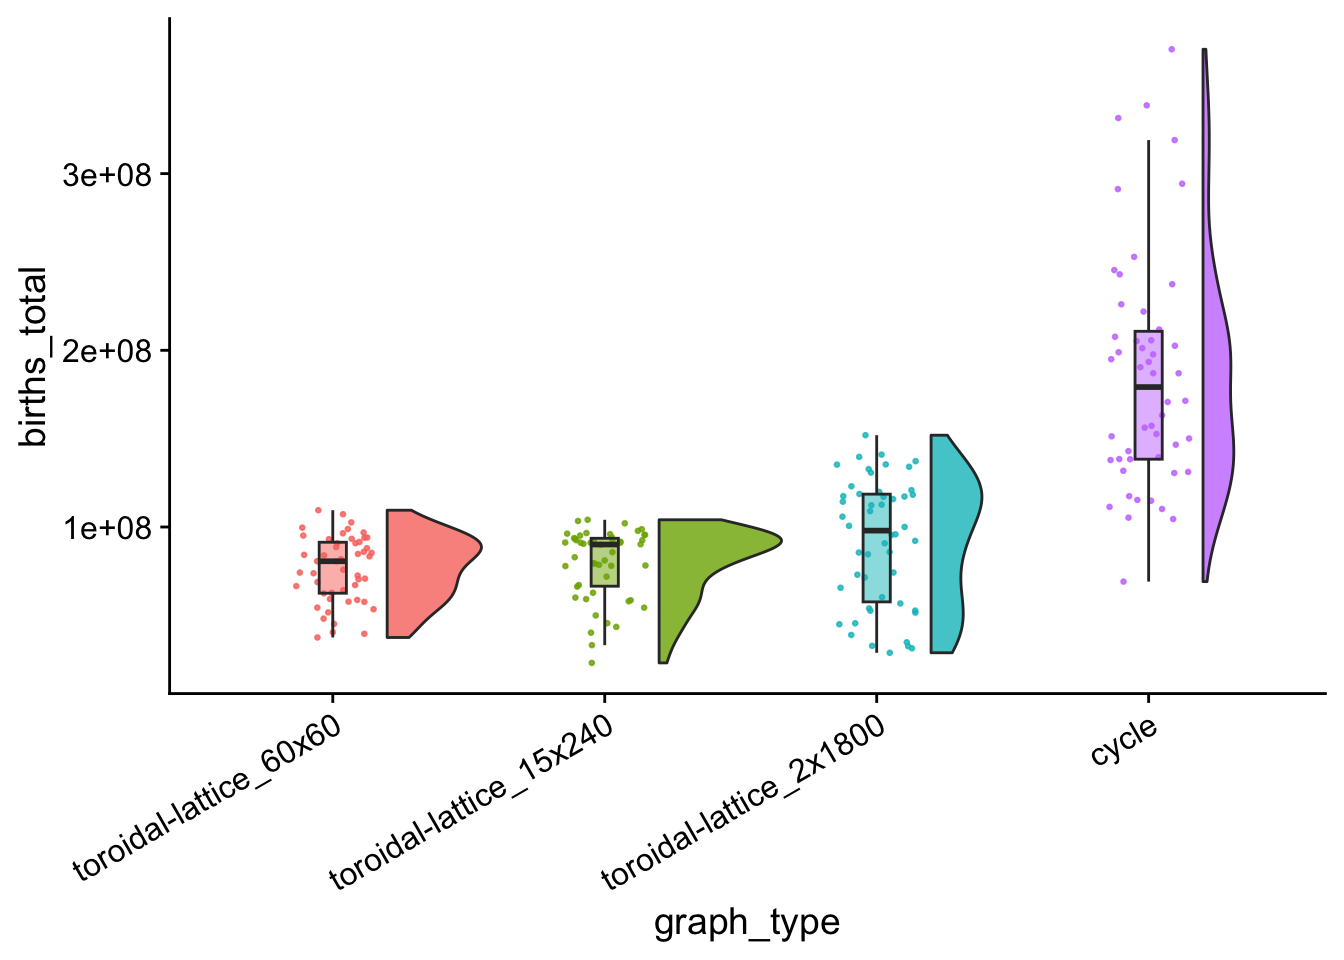
\includegraphics{supplemental-material_files/figure-latex/unnamed-chunk-106-1.pdf}

\hypertarget{variance-birth-counts-1}{%
\subsection{Variance birth Counts}\label{variance-birth-counts-1}}

\begin{Shaded}
\begin{Highlighting}[]
\NormalTok{birth\_counts\_var\_plt }\OtherTok{\textless{}{-}} \FunctionTok{ggplot}\NormalTok{(}
    \AttributeTok{data =}\NormalTok{ graph\_loc\_data\_summary,}
    \AttributeTok{mapping =} \FunctionTok{aes}\NormalTok{(}
      \AttributeTok{x =}\NormalTok{ graph\_type,}
      \AttributeTok{y =}\NormalTok{ births\_var,}
      \AttributeTok{fill =}\NormalTok{ graph\_type}
\NormalTok{    )}
\NormalTok{  ) }\SpecialCharTok{+}
  \FunctionTok{geom\_flat\_violin}\NormalTok{(}
    \AttributeTok{position =} \FunctionTok{position\_nudge}\NormalTok{(}\AttributeTok{x =}\NormalTok{ .}\DecValTok{2}\NormalTok{, }\AttributeTok{y =} \DecValTok{0}\NormalTok{),}
    \AttributeTok{alpha =}\NormalTok{ .}\DecValTok{8}
\NormalTok{  ) }\SpecialCharTok{+}
  \FunctionTok{geom\_point}\NormalTok{(}
    \AttributeTok{mapping=}\FunctionTok{aes}\NormalTok{(}\AttributeTok{color =}\NormalTok{ graph\_type),}
    \AttributeTok{position =} \FunctionTok{position\_jitter}\NormalTok{(}\AttributeTok{width =}\NormalTok{ .}\DecValTok{15}\NormalTok{),}
    \AttributeTok{size =}\NormalTok{ .}\DecValTok{5}\NormalTok{,}
    \AttributeTok{alpha =} \FloatTok{0.8}
\NormalTok{  ) }\SpecialCharTok{+}
  \FunctionTok{geom\_boxplot}\NormalTok{(}
    \AttributeTok{width =}\NormalTok{ .}\DecValTok{1}\NormalTok{,}
    \AttributeTok{outlier.shape =} \ConstantTok{NA}\NormalTok{,}
    \AttributeTok{alpha =} \FloatTok{0.5}
\NormalTok{  ) }\SpecialCharTok{+}
  \FunctionTok{theme}\NormalTok{(}
    \AttributeTok{legend.position =} \StringTok{"none"}\NormalTok{,}
    \AttributeTok{axis.text.x =} \FunctionTok{element\_text}\NormalTok{(}
      \AttributeTok{angle =} \DecValTok{30}\NormalTok{,}
      \AttributeTok{hjust =} \DecValTok{1}
\NormalTok{    )}
\NormalTok{  )}

\FunctionTok{ggsave}\NormalTok{(}
  \AttributeTok{filename =} \FunctionTok{paste0}\NormalTok{(plot\_dir, }\StringTok{"/birth\_counts\_var.pdf"}\NormalTok{),}
  \AttributeTok{plot =}\NormalTok{ birth\_counts\_var\_plt,}
  \AttributeTok{width =} \DecValTok{15}\NormalTok{,}
  \AttributeTok{height =} \DecValTok{10}
\NormalTok{)}

\NormalTok{birth\_counts\_var\_plt}
\end{Highlighting}
\end{Shaded}

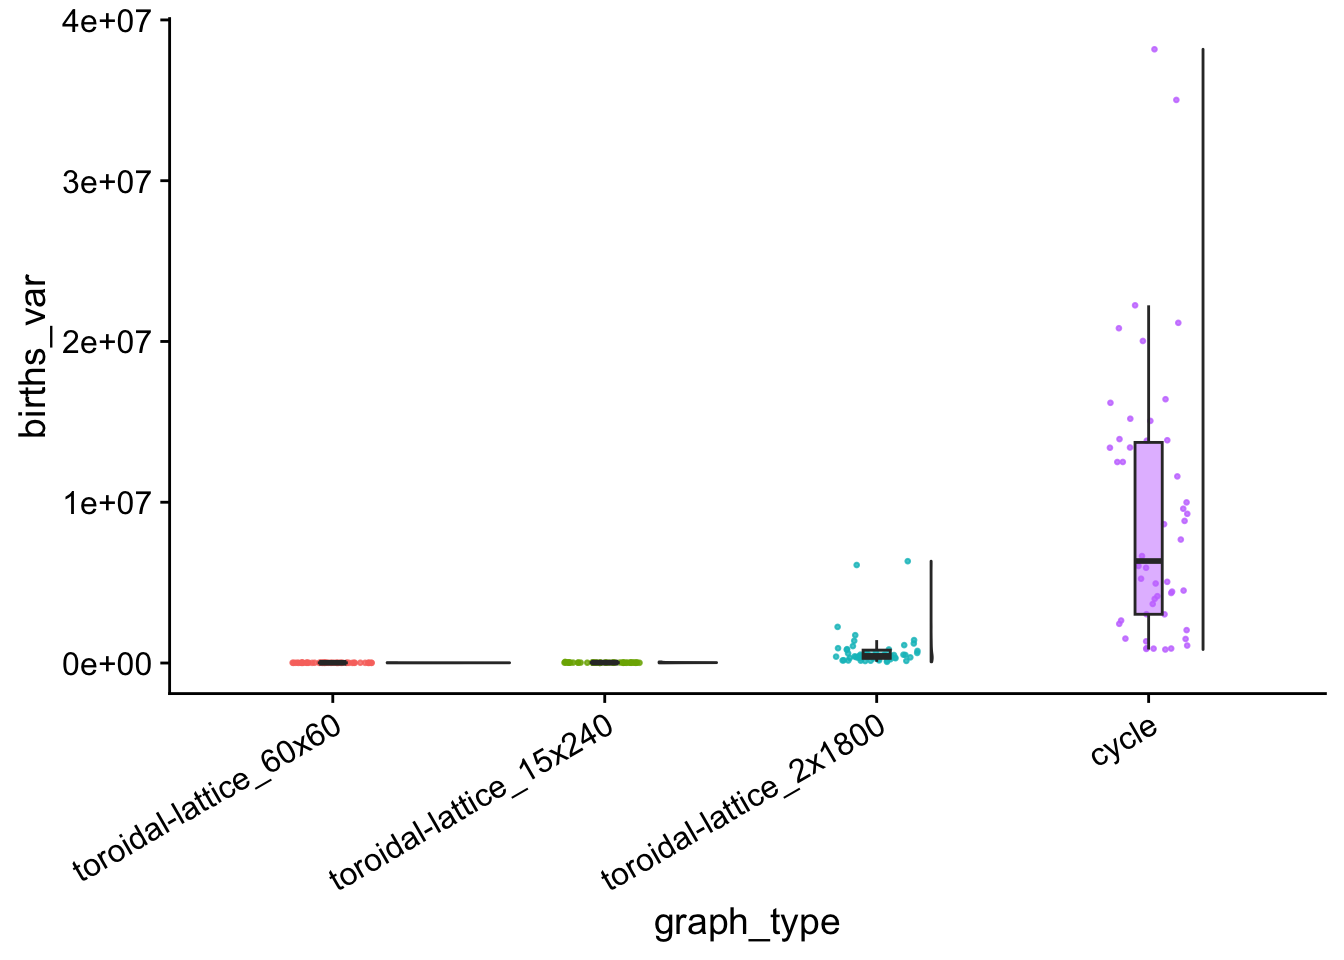
\includegraphics{supplemental-material_files/figure-latex/unnamed-chunk-107-1.pdf}

\hypertarget{task-appearances-total-1}{%
\subsection{Task appearances total}\label{task-appearances-total-1}}

\begin{Shaded}
\begin{Highlighting}[]
\NormalTok{task\_apps\_total\_plt }\OtherTok{\textless{}{-}} \FunctionTok{ggplot}\NormalTok{(}
    \AttributeTok{data =}\NormalTok{ graph\_loc\_data\_summary,}
    \AttributeTok{mapping =} \FunctionTok{aes}\NormalTok{(}
      \AttributeTok{x =}\NormalTok{ graph\_type,}
      \AttributeTok{y =}\NormalTok{ task\_apps\_total,}
      \AttributeTok{fill =}\NormalTok{ graph\_type}
\NormalTok{    )}
\NormalTok{  ) }\SpecialCharTok{+}
  \FunctionTok{geom\_flat\_violin}\NormalTok{(}
    \AttributeTok{position =} \FunctionTok{position\_nudge}\NormalTok{(}\AttributeTok{x =}\NormalTok{ .}\DecValTok{2}\NormalTok{, }\AttributeTok{y =} \DecValTok{0}\NormalTok{),}
    \AttributeTok{alpha =}\NormalTok{ .}\DecValTok{8}
\NormalTok{  ) }\SpecialCharTok{+}
  \FunctionTok{geom\_point}\NormalTok{(}
    \AttributeTok{mapping=}\FunctionTok{aes}\NormalTok{(}\AttributeTok{color =}\NormalTok{ graph\_type),}
    \AttributeTok{position =} \FunctionTok{position\_jitter}\NormalTok{(}\AttributeTok{width =}\NormalTok{ .}\DecValTok{15}\NormalTok{),}
    \AttributeTok{size =}\NormalTok{ .}\DecValTok{5}\NormalTok{,}
    \AttributeTok{alpha =} \FloatTok{0.8}
\NormalTok{  ) }\SpecialCharTok{+}
  \FunctionTok{geom\_boxplot}\NormalTok{(}
    \AttributeTok{width =}\NormalTok{ .}\DecValTok{1}\NormalTok{,}
    \AttributeTok{outlier.shape =} \ConstantTok{NA}\NormalTok{,}
    \AttributeTok{alpha =} \FloatTok{0.5}
\NormalTok{  ) }\SpecialCharTok{+}
  \FunctionTok{theme}\NormalTok{(}
    \AttributeTok{legend.position =} \StringTok{"none"}\NormalTok{,}
    \AttributeTok{axis.text.x =} \FunctionTok{element\_text}\NormalTok{(}
      \AttributeTok{angle =} \DecValTok{30}\NormalTok{,}
      \AttributeTok{hjust =} \DecValTok{1}
\NormalTok{    )}
\NormalTok{  )}

\FunctionTok{ggsave}\NormalTok{(}
  \AttributeTok{filename =} \FunctionTok{paste0}\NormalTok{(plot\_dir, }\StringTok{"/task\_apps\_total.pdf"}\NormalTok{),}
  \AttributeTok{plot =}\NormalTok{ task\_apps\_total\_plt,}
  \AttributeTok{width =} \DecValTok{15}\NormalTok{,}
  \AttributeTok{height =} \DecValTok{10}
\NormalTok{)}

\NormalTok{task\_apps\_total\_plt}
\end{Highlighting}
\end{Shaded}

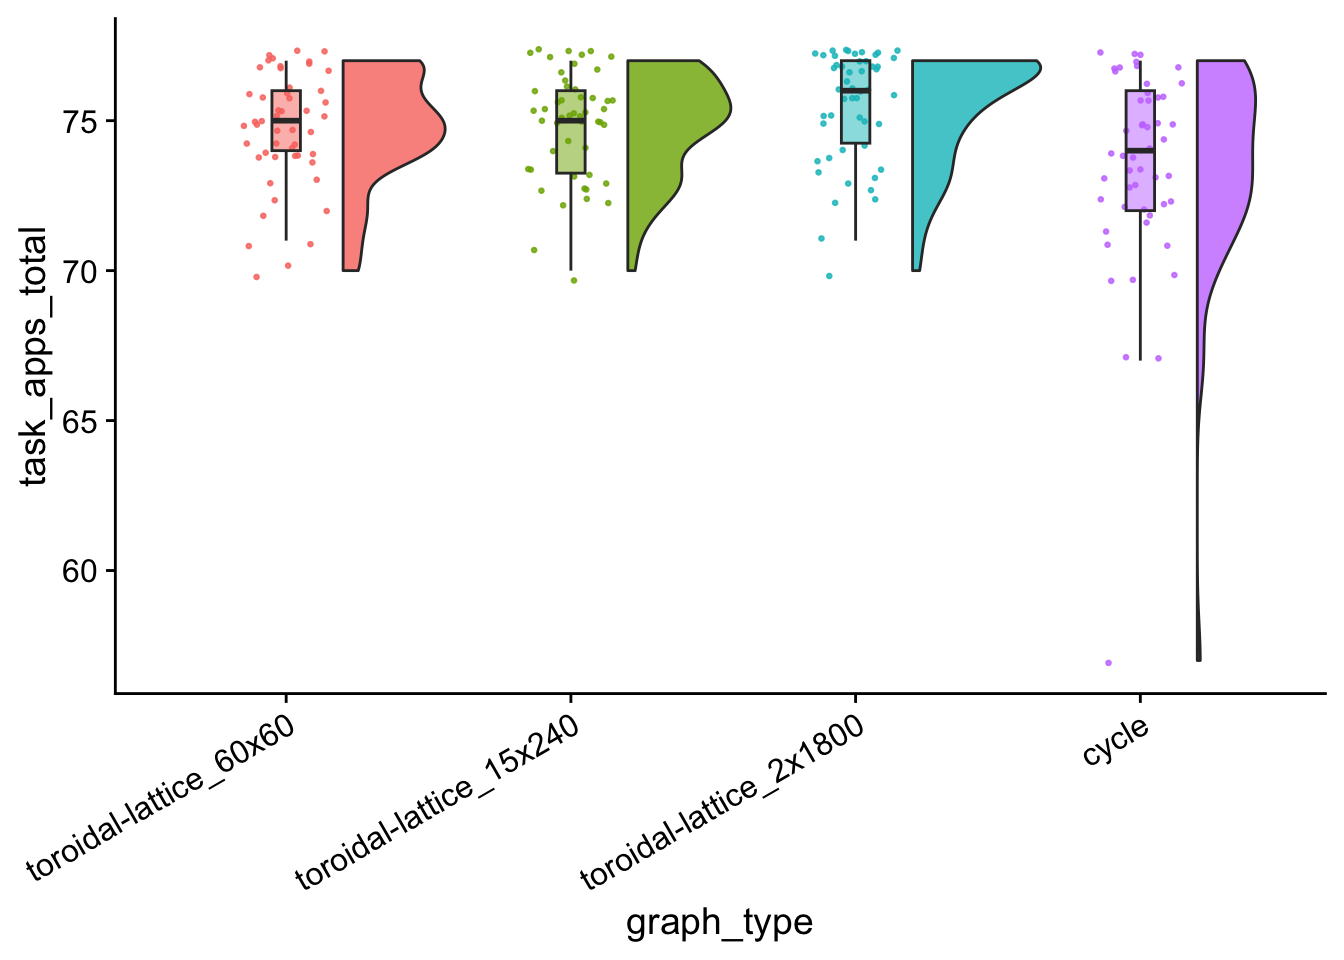
\includegraphics{supplemental-material_files/figure-latex/unnamed-chunk-108-1.pdf}

\begin{Shaded}
\begin{Highlighting}[]
\FunctionTok{kruskal.test}\NormalTok{(}
  \AttributeTok{formula =}\NormalTok{ task\_apps\_total }\SpecialCharTok{\textasciitilde{}}\NormalTok{ graph\_type,}
  \AttributeTok{data =}\NormalTok{ graph\_loc\_data\_summary}
\NormalTok{)}
\end{Highlighting}
\end{Shaded}

\begin{verbatim}
## 
##  Kruskal-Wallis rank sum test
## 
## data:  task_apps_total by graph_type
## Kruskal-Wallis chi-squared = 15.09, df = 3, p-value = 0.001742
\end{verbatim}

\begin{Shaded}
\begin{Highlighting}[]
\NormalTok{wc\_results }\OtherTok{\textless{}{-}} \FunctionTok{pairwise.wilcox.test}\NormalTok{(}
  \AttributeTok{x =}\NormalTok{ graph\_loc\_data\_summary}\SpecialCharTok{$}\NormalTok{task\_apps\_total,}
  \AttributeTok{g =}\NormalTok{ graph\_loc\_data\_summary}\SpecialCharTok{$}\NormalTok{graph\_type,}
  \AttributeTok{p.adjust.method   =} \StringTok{"holm"}\NormalTok{,}
  \AttributeTok{exact =} \ConstantTok{FALSE}

\NormalTok{)}
\NormalTok{wc\_results}
\end{Highlighting}
\end{Shaded}

\begin{verbatim}
## 
##  Pairwise comparisons using Wilcoxon rank sum test with continuity correction 
## 
## data:  graph_loc_data_summary$task_apps_total and graph_loc_data_summary$graph_type 
## 
##                         toroidal-lattice_60x60 toroidal-lattice_15x240
## toroidal-lattice_15x240 0.771                  -                      
## toroidal-lattice_2x1800 0.125                  0.125                  
## cycle                   0.128                  0.125                  
##                         toroidal-lattice_2x1800
## toroidal-lattice_15x240 -                      
## toroidal-lattice_2x1800 -                      
## cycle                   0.002                  
## 
## P value adjustment method: holm
\end{verbatim}

\hypertarget{morans-i-results}{%
\section{Moran's I results}\label{morans-i-results}}

\begin{Shaded}
\begin{Highlighting}[]
\CommentTok{\# Load summary data from final update}
\NormalTok{morans\_i\_data\_path }\OtherTok{\textless{}{-}} \FunctionTok{paste}\NormalTok{(}
\NormalTok{  working\_directory,}
  \StringTok{"data"}\NormalTok{,}
  \StringTok{"morans\_i.csv"}\NormalTok{,}
  \AttributeTok{sep =} \StringTok{"/"}
\NormalTok{)}
\NormalTok{morans\_i\_data }\OtherTok{\textless{}{-}} \FunctionTok{read\_csv}\NormalTok{(morans\_i\_data\_path)}

\NormalTok{morans\_i\_data }\OtherTok{\textless{}{-}}\NormalTok{ morans\_i\_data }\SpecialCharTok{\%\textgreater{}\%}
  \FunctionTok{mutate}\NormalTok{(}
    \AttributeTok{graph\_type =} \FunctionTok{str\_split\_i}\NormalTok{(}
\NormalTok{      graph\_file,}
      \AttributeTok{pattern =} \StringTok{".mat"}\NormalTok{,}
      \DecValTok{1}
\NormalTok{    )}
\NormalTok{  ) }\SpecialCharTok{\%\textgreater{}\%}
  \FunctionTok{mutate}\NormalTok{(}
    \AttributeTok{graph\_type =} \FunctionTok{factor}\NormalTok{(}
\NormalTok{      graph\_type,}
      \AttributeTok{levels =} \FunctionTok{c}\NormalTok{(}
        \StringTok{"toroidal{-}lattice\_60x60"}\NormalTok{,}
        \StringTok{"toroidal{-}lattice\_30x120"}\NormalTok{,}
        \StringTok{"toroidal{-}lattice\_15x240"}\NormalTok{,}
        \StringTok{"toroidal{-}lattice\_4x900"}\NormalTok{,}
        \StringTok{"toroidal{-}lattice\_3x1200"}\NormalTok{,}
        \StringTok{"toroidal{-}lattice\_2x1800"}\NormalTok{,}
        \StringTok{"cycle"}
\NormalTok{      )}
\NormalTok{    ),}
    \AttributeTok{seed =} \FunctionTok{as.factor}\NormalTok{(seed)}
\NormalTok{  ) }\SpecialCharTok{\%\textgreater{}\%}
  \FunctionTok{filter}\NormalTok{(}
\NormalTok{    graph\_type }\SpecialCharTok{\%in\%}\NormalTok{ focal\_graphs}
\NormalTok{  )}
\end{Highlighting}
\end{Shaded}

\hypertarget{clustered-task-appearances}{%
\subsection{Clustered task appearances}\label{clustered-task-appearances}}

Summarize statistically significant runs where I \textgreater{} 0.

\begin{Shaded}
\begin{Highlighting}[]
\CommentTok{\# Identify number of runs where distribution of task appearances is more}
\CommentTok{\# clustered than we would expect by chance.}
\NormalTok{clustered\_counts }\OtherTok{\textless{}{-}}\NormalTok{ morans\_i\_data }\SpecialCharTok{\%\textgreater{}\%}
  \FunctionTok{filter}\NormalTok{(}
\NormalTok{    (task\_morans\_i }\SpecialCharTok{\textgreater{}} \DecValTok{0}\NormalTok{) }\SpecialCharTok{\&}\NormalTok{ (task\_p\_val }\SpecialCharTok{\textless{}=} \FloatTok{0.05}\NormalTok{)}
\NormalTok{  ) }\SpecialCharTok{\%\textgreater{}\%}
  \FunctionTok{group\_by}\NormalTok{(graph\_type) }\SpecialCharTok{\%\textgreater{}\%}
  \FunctionTok{summarize}\NormalTok{(}
    \AttributeTok{n =} \FunctionTok{n}\NormalTok{()}
\NormalTok{  )}
\end{Highlighting}
\end{Shaded}

\begin{Shaded}
\begin{Highlighting}[]
\NormalTok{tasks\_clustered\_plt }\OtherTok{\textless{}{-}}\NormalTok{ clustered\_counts }\SpecialCharTok{\%\textgreater{}\%}
  \FunctionTok{ggplot}\NormalTok{(}
    \FunctionTok{aes}\NormalTok{(}
      \AttributeTok{x =}\NormalTok{ graph\_type,}
      \AttributeTok{y =}\NormalTok{ n,}
      \AttributeTok{color =}\NormalTok{ graph\_type,}
      \AttributeTok{fill =}\NormalTok{ graph\_type}
\NormalTok{    )}
\NormalTok{  ) }\SpecialCharTok{+}
  \FunctionTok{geom\_col}\NormalTok{() }\SpecialCharTok{+}
  \FunctionTok{theme}\NormalTok{(}
    \AttributeTok{legend.position =} \StringTok{"none"}\NormalTok{,}
    \AttributeTok{axis.text.x =} \FunctionTok{element\_text}\NormalTok{(}
      \AttributeTok{angle =} \DecValTok{30}\NormalTok{,}
      \AttributeTok{hjust =} \DecValTok{1}
\NormalTok{    )}
\NormalTok{  )}

\FunctionTok{ggsave}\NormalTok{(}
  \AttributeTok{filename =} \FunctionTok{paste0}\NormalTok{(plot\_dir, }\StringTok{"/tasks\_clustered\_plt.pdf"}\NormalTok{),}
  \AttributeTok{plot =}\NormalTok{ tasks\_clustered\_plt,}
  \AttributeTok{width =} \DecValTok{15}\NormalTok{,}
  \AttributeTok{height =} \DecValTok{10}
\NormalTok{)}

\NormalTok{tasks\_clustered\_plt}
\end{Highlighting}
\end{Shaded}

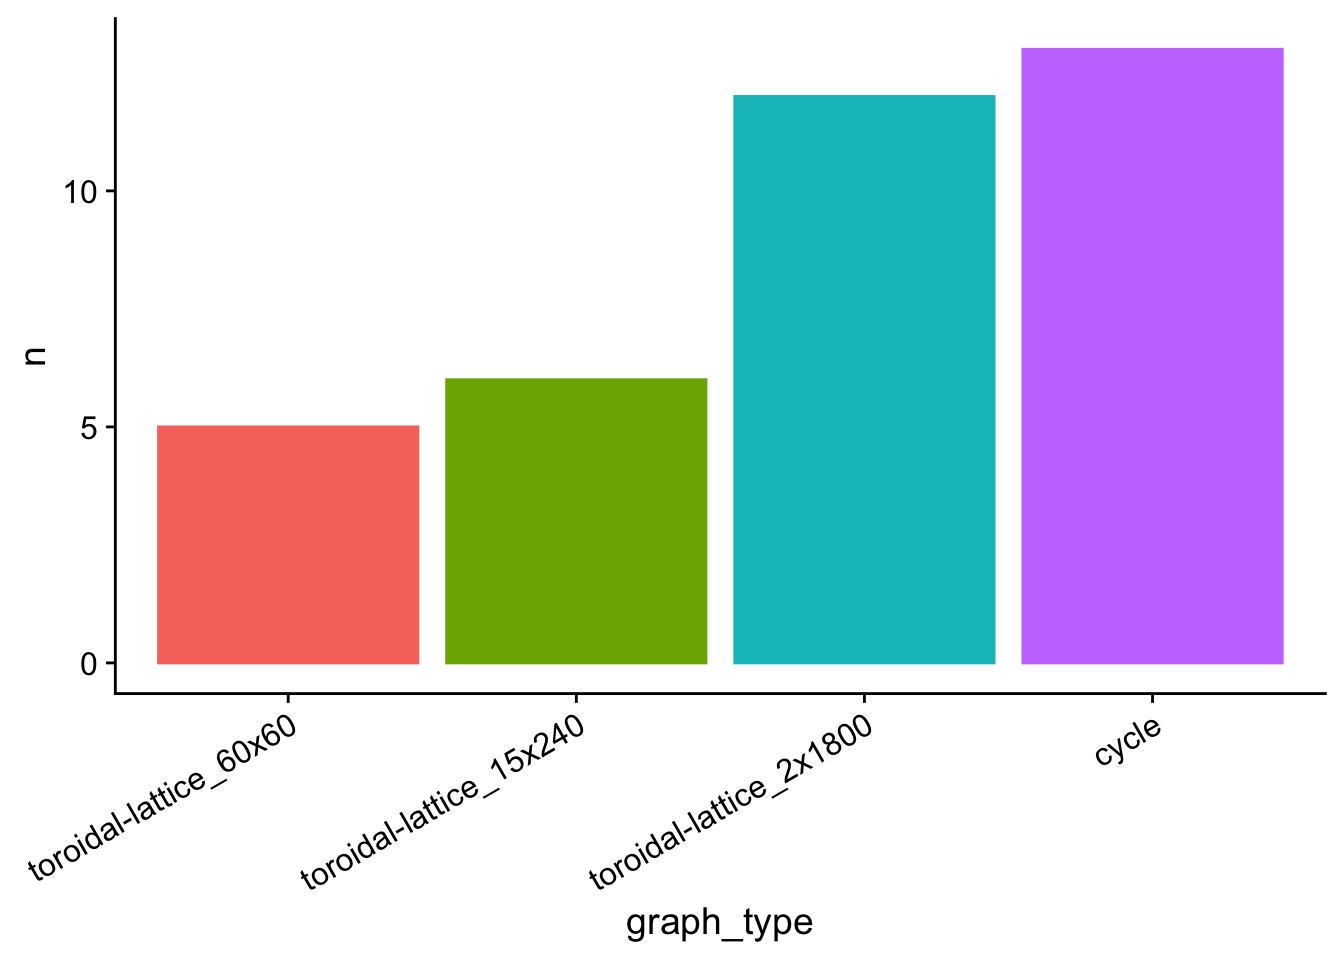
\includegraphics{supplemental-material_files/figure-latex/unnamed-chunk-112-1.pdf}

\begin{Shaded}
\begin{Highlighting}[]
\NormalTok{tasks\_clustered\_i\_vals\_plt }\OtherTok{\textless{}{-}}\NormalTok{ morans\_i\_data }\SpecialCharTok{\%\textgreater{}\%}
  \FunctionTok{filter}\NormalTok{((task\_morans\_i }\SpecialCharTok{\textgreater{}} \DecValTok{0}\NormalTok{) }\SpecialCharTok{\&}\NormalTok{ (task\_p\_val }\SpecialCharTok{\textless{}=} \FloatTok{0.05}\NormalTok{)) }\SpecialCharTok{\%\textgreater{}\%}
  \FunctionTok{ggplot}\NormalTok{(}
    \AttributeTok{mapping =} \FunctionTok{aes}\NormalTok{(}
      \AttributeTok{x =}\NormalTok{ graph\_type,}
      \AttributeTok{y =}\NormalTok{ task\_morans\_i,}
      \AttributeTok{fill =}\NormalTok{ graph\_type}
\NormalTok{    )}
\NormalTok{  ) }\SpecialCharTok{+}
  \FunctionTok{geom\_flat\_violin}\NormalTok{(}
    \AttributeTok{position =} \FunctionTok{position\_nudge}\NormalTok{(}\AttributeTok{x =}\NormalTok{ .}\DecValTok{2}\NormalTok{, }\AttributeTok{y =} \DecValTok{0}\NormalTok{),}
    \AttributeTok{alpha =}\NormalTok{ .}\DecValTok{8}
\NormalTok{  ) }\SpecialCharTok{+}
  \FunctionTok{geom\_point}\NormalTok{(}
    \AttributeTok{mapping=}\FunctionTok{aes}\NormalTok{(}\AttributeTok{color =}\NormalTok{ graph\_type),}
    \AttributeTok{position =} \FunctionTok{position\_jitter}\NormalTok{(}\AttributeTok{width =}\NormalTok{ .}\DecValTok{15}\NormalTok{),}
    \AttributeTok{size =}\NormalTok{ .}\DecValTok{5}\NormalTok{,}
    \AttributeTok{alpha =} \FloatTok{0.8}
\NormalTok{  ) }\SpecialCharTok{+}
  \FunctionTok{geom\_boxplot}\NormalTok{(}
    \AttributeTok{width =}\NormalTok{ .}\DecValTok{1}\NormalTok{,}
    \AttributeTok{outlier.shape =} \ConstantTok{NA}\NormalTok{,}
    \AttributeTok{alpha =} \FloatTok{0.5}
\NormalTok{  ) }\SpecialCharTok{+}
  \FunctionTok{theme}\NormalTok{(}
    \AttributeTok{legend.position =} \StringTok{"none"}\NormalTok{,}
    \AttributeTok{axis.text.x =} \FunctionTok{element\_text}\NormalTok{(}
      \AttributeTok{angle =} \DecValTok{30}\NormalTok{,}
      \AttributeTok{hjust =} \DecValTok{1}
\NormalTok{    )}
\NormalTok{  )}

\FunctionTok{ggsave}\NormalTok{(}
  \AttributeTok{filename =} \FunctionTok{paste0}\NormalTok{(plot\_dir, }\StringTok{"/tasks\_clustered\_i\_vals\_plt.pdf"}\NormalTok{),}
  \AttributeTok{plot =}\NormalTok{ tasks\_clustered\_i\_vals\_plt,}
  \AttributeTok{width =} \DecValTok{15}\NormalTok{,}
  \AttributeTok{height =} \DecValTok{10}
\NormalTok{)}

\NormalTok{tasks\_clustered\_i\_vals\_plt}
\end{Highlighting}
\end{Shaded}

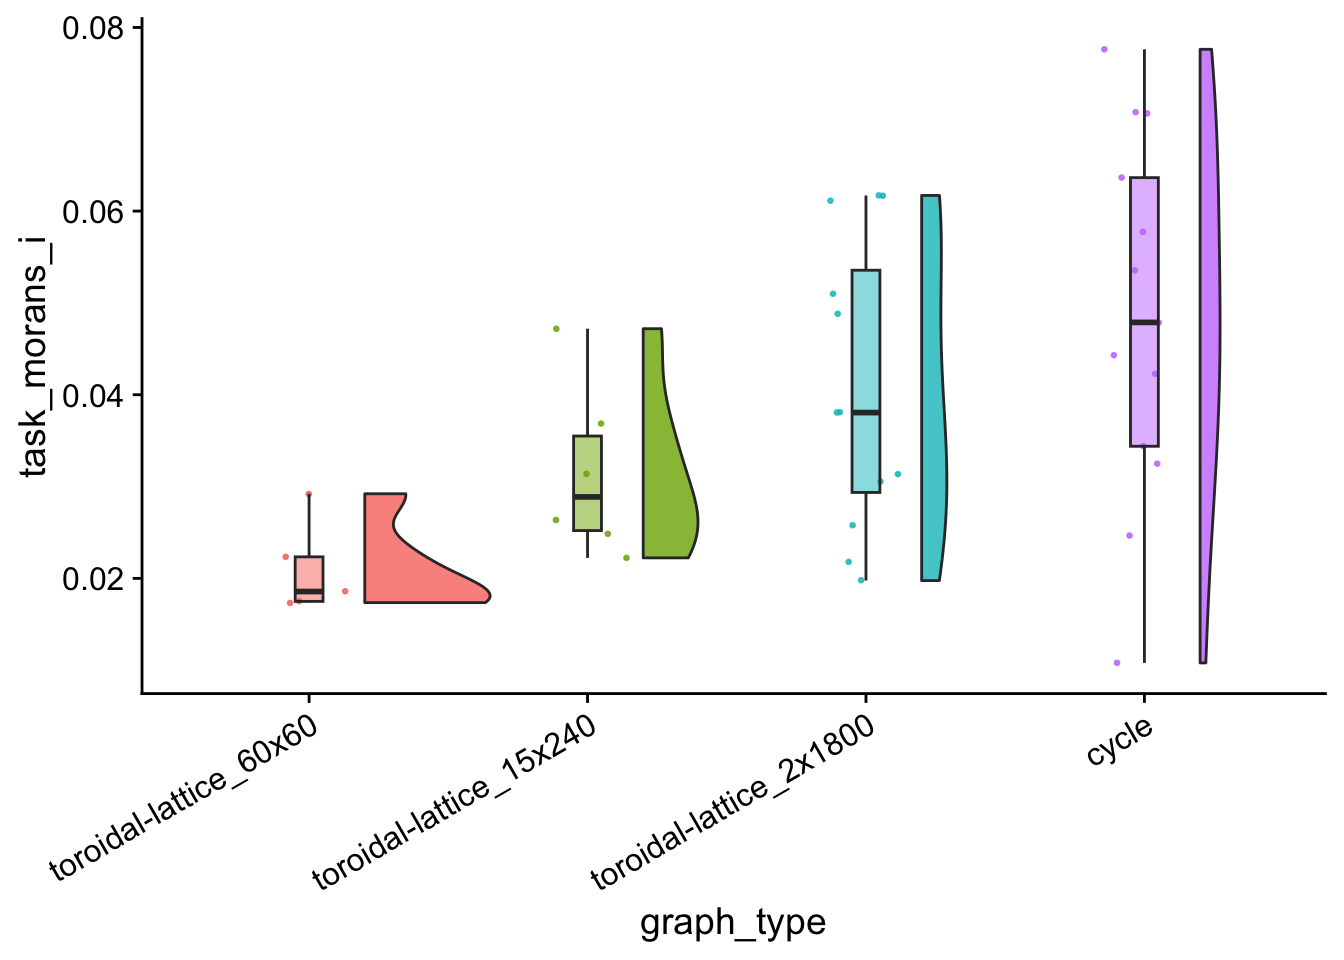
\includegraphics{supplemental-material_files/figure-latex/unnamed-chunk-113-1.pdf}

\hypertarget{clustered-birth-counts}{%
\subsection{Clustered birth counts}\label{clustered-birth-counts}}

\begin{Shaded}
\begin{Highlighting}[]
\NormalTok{births\_clustered\_plot }\OtherTok{\textless{}{-}}\NormalTok{ morans\_i\_data }\SpecialCharTok{\%\textgreater{}\%}
  \FunctionTok{filter}\NormalTok{((birth\_morans\_i }\SpecialCharTok{\textgreater{}} \DecValTok{0}\NormalTok{) }\SpecialCharTok{\&}\NormalTok{ (birth\_p\_val }\SpecialCharTok{\textless{}=} \FloatTok{0.05}\NormalTok{)) }\SpecialCharTok{\%\textgreater{}\%}
  \FunctionTok{ggplot}\NormalTok{(}
    \FunctionTok{aes}\NormalTok{(}
      \AttributeTok{x =}\NormalTok{ graph\_type,}
      \AttributeTok{color =}\NormalTok{ graph\_type,}
      \AttributeTok{fill =}\NormalTok{ graph\_type}
\NormalTok{    )}
\NormalTok{  ) }\SpecialCharTok{+}
  \FunctionTok{geom\_bar}\NormalTok{() }\SpecialCharTok{+}
  \FunctionTok{theme}\NormalTok{(}
    \AttributeTok{legend.position =} \StringTok{"none"}\NormalTok{,}
    \AttributeTok{axis.text.x =} \FunctionTok{element\_text}\NormalTok{(}
      \AttributeTok{angle =} \DecValTok{30}\NormalTok{,}
      \AttributeTok{hjust =} \DecValTok{1}
\NormalTok{    )}
\NormalTok{  )}

\FunctionTok{ggsave}\NormalTok{(}
  \AttributeTok{filename =} \FunctionTok{paste0}\NormalTok{(plot\_dir, }\StringTok{"/births\_clustered\_plot.pdf"}\NormalTok{),}
  \AttributeTok{plot =}\NormalTok{ births\_clustered\_plot,}
  \AttributeTok{width =} \DecValTok{15}\NormalTok{,}
  \AttributeTok{height =} \DecValTok{10}
\NormalTok{)}

\NormalTok{births\_clustered\_plot}
\end{Highlighting}
\end{Shaded}

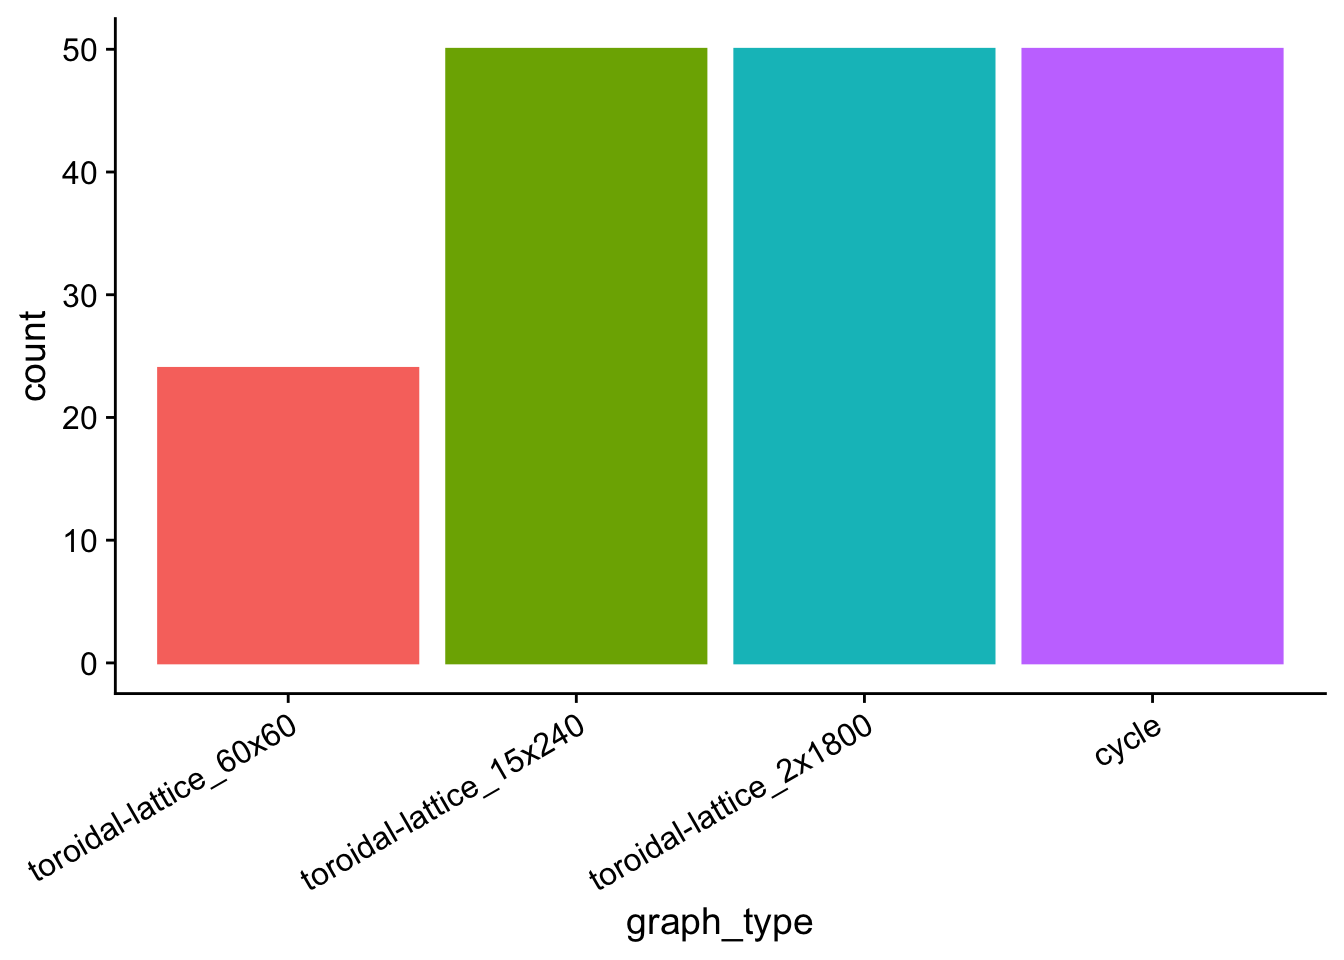
\includegraphics{supplemental-material_files/figure-latex/unnamed-chunk-114-1.pdf}

\begin{Shaded}
\begin{Highlighting}[]
\NormalTok{birth\_clustered\_i\_vals\_plt }\OtherTok{\textless{}{-}}\NormalTok{ morans\_i\_data }\SpecialCharTok{\%\textgreater{}\%}
  \FunctionTok{filter}\NormalTok{((birth\_morans\_i }\SpecialCharTok{\textgreater{}} \DecValTok{0}\NormalTok{) }\SpecialCharTok{\&}\NormalTok{ (birth\_p\_val }\SpecialCharTok{\textless{}=} \FloatTok{0.05}\NormalTok{)) }\SpecialCharTok{\%\textgreater{}\%}
  \FunctionTok{ggplot}\NormalTok{(}
    \AttributeTok{mapping =} \FunctionTok{aes}\NormalTok{(}
      \AttributeTok{x =}\NormalTok{ graph\_type,}
      \AttributeTok{y =}\NormalTok{ birth\_morans\_i,}
      \AttributeTok{fill =}\NormalTok{ graph\_type}
\NormalTok{    )}
\NormalTok{  ) }\SpecialCharTok{+}
  \FunctionTok{geom\_flat\_violin}\NormalTok{(}
    \AttributeTok{position =} \FunctionTok{position\_nudge}\NormalTok{(}\AttributeTok{x =}\NormalTok{ .}\DecValTok{2}\NormalTok{, }\AttributeTok{y =} \DecValTok{0}\NormalTok{),}
    \AttributeTok{alpha =}\NormalTok{ .}\DecValTok{8}
\NormalTok{  ) }\SpecialCharTok{+}
  \FunctionTok{geom\_point}\NormalTok{(}
    \AttributeTok{mapping=}\FunctionTok{aes}\NormalTok{(}\AttributeTok{color =}\NormalTok{ graph\_type),}
    \AttributeTok{position =} \FunctionTok{position\_jitter}\NormalTok{(}\AttributeTok{width =}\NormalTok{ .}\DecValTok{15}\NormalTok{),}
    \AttributeTok{size =}\NormalTok{ .}\DecValTok{5}\NormalTok{,}
    \AttributeTok{alpha =} \FloatTok{0.8}
\NormalTok{  ) }\SpecialCharTok{+}
  \FunctionTok{geom\_boxplot}\NormalTok{(}
    \AttributeTok{width =}\NormalTok{ .}\DecValTok{1}\NormalTok{,}
    \AttributeTok{outlier.shape =} \ConstantTok{NA}\NormalTok{,}
    \AttributeTok{alpha =} \FloatTok{0.5}
\NormalTok{  ) }\SpecialCharTok{+}
  \FunctionTok{theme}\NormalTok{(}
    \AttributeTok{legend.position =} \StringTok{"none"}\NormalTok{,}
    \AttributeTok{axis.text.x =} \FunctionTok{element\_text}\NormalTok{(}
      \AttributeTok{angle =} \DecValTok{30}\NormalTok{,}
      \AttributeTok{hjust =} \DecValTok{1}
\NormalTok{    )}
\NormalTok{  )}

\FunctionTok{ggsave}\NormalTok{(}
  \AttributeTok{filename =} \FunctionTok{paste0}\NormalTok{(plot\_dir, }\StringTok{"/birth\_clustered\_i\_vals\_plt.pdf"}\NormalTok{),}
  \AttributeTok{plot =}\NormalTok{ birth\_clustered\_i\_vals\_plt,}
  \AttributeTok{width =} \DecValTok{15}\NormalTok{,}
  \AttributeTok{height =} \DecValTok{10}
\NormalTok{)}

\NormalTok{birth\_clustered\_i\_vals\_plt}
\end{Highlighting}
\end{Shaded}

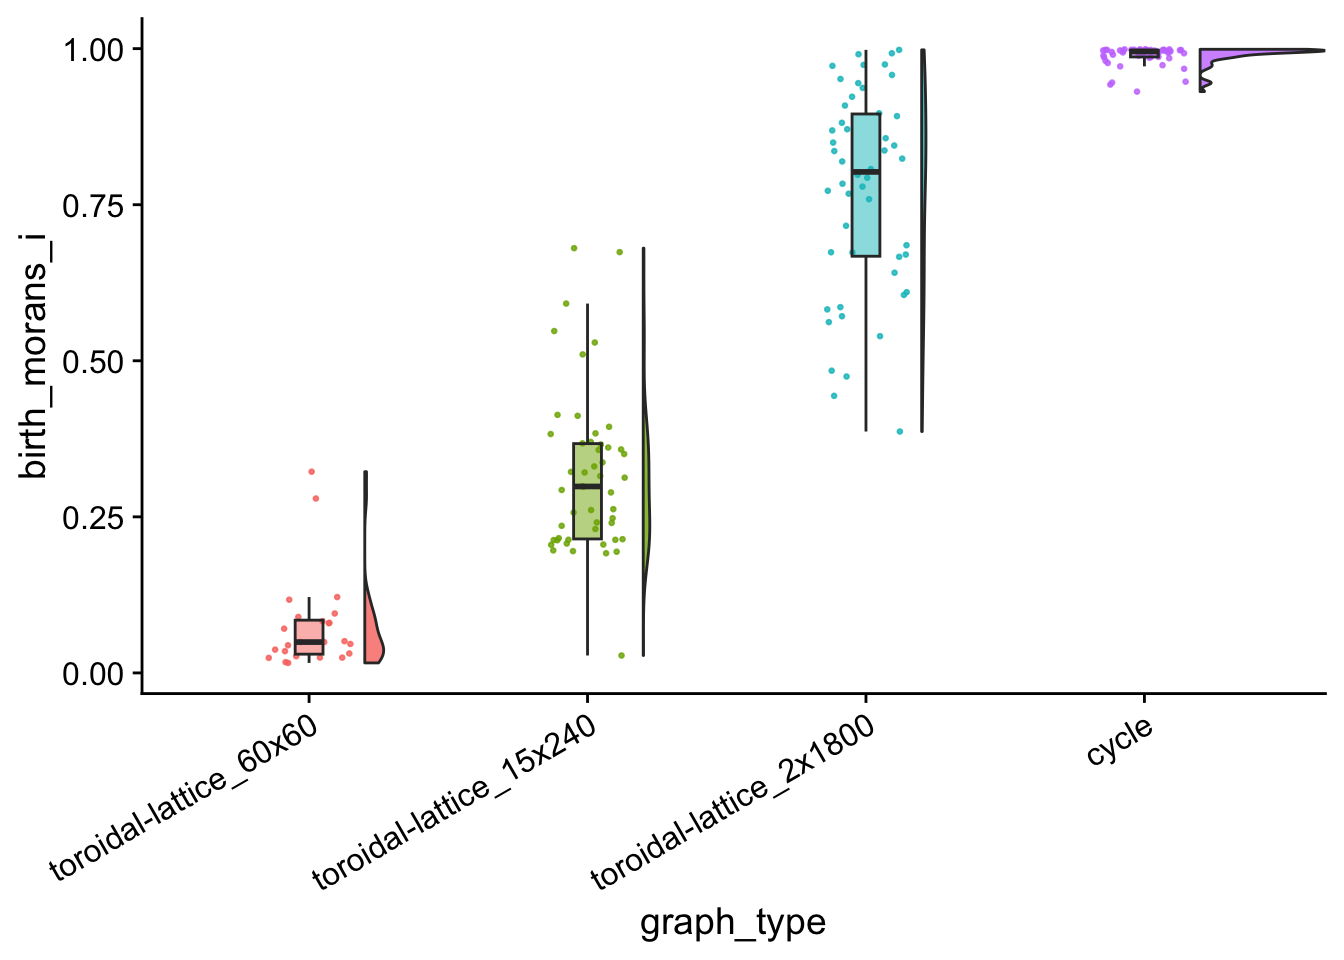
\includegraphics{supplemental-material_files/figure-latex/unnamed-chunk-115-1.pdf}

  \bibliography{packages.bib,supplemental.bib}

\end{document}
